
\chapter*{Preface}
\markboth{Preface}{Preface}
\addcontentsline{toc}{chapter}{\numberline{}Preface}

This is a book about prime numbers, congruences, secret messages, and
elliptic curves that you can read cover to cover.  It grew out of
undergraduate courses that the author taught at Harvard, UC San Diego,
and the University of Washington.

The systematic study of number theory was initiated around 300{\sc B.C.} when
Euclid proved that there are infinitely many prime numbers, and also
cleverly deduced the fundamental theorem of arithmetic, which asserts
that every positive integer factors uniquely as a product of primes.
Over a thousand years later (around 972{\sc A.D.}) Arab mathematicians
formulated the {\em congruent number problem} that asks for a way to
decide whether or not a given positive integer $n$ is the area of a
right triangle, all three of whose sides are rational numbers.  Then
another thousand years later (in 1976), Diffie and Hellman introduced the
first ever public-key cryptosystem, which enabled two people to
communicate secretely over a public communications channel with no
predetermined secret; this invention and the ones that followed it
revolutionized the world of digital communication.  In the 1980s and
1990s, elliptic curves revolutionized number theory, providing
striking new insights into the congruent number problem, primality
testing, public-key cryptography, attacks on public-key systems, and
playing a central role in Andrew Wiles' resolution of Fermat's Last
Theorem.

Today, pure and applied number theory is an exciting mix of
simultaneously broad and deep theory, which is constantly informed and
motivated by algorithms and explicit computation.  Active research is
underway that promises to resolve the congruent number problem, deepen
our understanding into the structure of prime numbers, and both
challenge and improve our ability to communicate securely.  The goal
of this book is to bring the reader closer to this world.

The reader is strongly encouraged to do every exercise in this book,
checking their answers in the back (where many, but not all, solutions
are given).  Also, throughout the text there, are examples of
calculations done using the powerful free open source mathematical
software system Sage (\url{http://www.sagemath.org}), and the reader
should try every such example and experiment with similar examples.

\vspace{1.5ex}\noindent{}{\bf Background.}  The reader should know how
to read and write mathematical proofs and must know the basics of
groups, rings, and fields.  Thus, the prerequisites for this book are
more than the prerequisites for most elementary number theory books,
while still being aimed at undergraduates.

\vspace{1.5ex}\noindent{}{\bf Notation and Conventions.}  We let
$\N=\{1,2,3,\ldots\}$ denote the natural numbers, and use the standard
notation $\Z$, $\Q$, $\R$, and $\C$ for the rings of integer,
rational, real, and complex numbers, respectively.\index{notation} In
this book, we will use the words proposition, theorem, lemma, and
corollary as follows.  Usually a proposition is a less important or
less fundamental assertion, a theorem is a deeper culmination of ideas, a
lemma is something that we will use later in this book to prove a
proposition or theorem, and a corollary is an easy consequence of a
proposition, theorem, or lemma.   More difficult exercises are marked
with a (*).

\vspace{1.5ex}\noindent{}{\bf Acknowledgements.} I would like to thank
Brian Conrad, Carl Pomerance, and Ken Ribet for many clarifying
comments and suggestions.  Baurzhan Bektemirov, Lawrence
Cabusora, and Keith Conrad read drafts of this book and made many
comments, and Carl Witty commented extensively on the first two
chapters.  Frank Calegari used the course when teaching Math 124 at
Harvard, and he and his students provided much feedback.  Noam Elkies
made comments and suggested \exref{ch:reciprocity}{ex:rec8}.  Seth
Kleinerman wrote a version of Section~\ref{sec:contfrac_e} as a class
project.  Hendrik Lenstra made helpful remarks about how to present
his factorization algorithm.  Michael Abshoff, Sabmit Dasgupta, David
Joyner, Arthur Patterson, George Stephanides, Kevin Stern, Eve
Thompson, Ting-You Wang, and Heidi Williams all suggested corrections.
I also benefited from conversations with Henry Cohn and David Savitt.
I used \sage (\cite{sage}), emacs, and \LaTeX{} in the preparation of
this book.

% Stephanides of University of Macedonia
%Heidi.L.Williams@Dartmouth.EDU


\cleardoublepage
\pagenumbering{arabic}
%%%%%%%%%%%%%%%%%%%%%%%%%%%%%%%%%%%%%%%%%%%%%%%%%%%%%%%%%%%%%%%%%%%%%%%
%%
%% Chapter: Prime Numbers
%%
%%%%%%%%%%%%%%%%%%%%%%%%%%%%%%%%%%%%%%%%%%%%%%%%%%%%%%%%%%%%%%%%%%%%%%%

\chapter{Prime Numbers}
\label{ch:prime}
Every positive integer can be written uniquely as a product of prime
numbers, e.g., $100 = 2^2 \cdot 5^2$.  This is surprisingly difficult
to prove, as we will see below.  Even more astounding is that actually
{\em finding} a way to write certain 1,000-digit numbers as a product
of primes seems out of the reach of present technology, an observation
that is used by millions of people every day when they buy things
online.

Since prime numbers are the building blocks of integers, it is
natural to wonder how the primes are distributed among the integers.
\begin{quote}
  ``There are two facts about the distribution of prime numbers. The
  first is that, [they are] the most arbitrary and ornery objects
  studied by mathematicians: they grow like weeds among the natural
  numbers, seeming to obey no other law than that of chance, and
  nobody can predict where the next one will sprout. The second fact
  is even more astonishing, for it states just the opposite: that the
  prime numbers exhibit stunning regularity, that there are laws
  governing their behavior, and that they obey these laws with almost
  military precision.''\\\mbox{} \hspace{2in} --- Don Zagier \cite{zagier:primes50}
\end{quote}
The Riemann Hypothesis, which is the most famous unsolved problem in
number theory, postulates a very precise answer to the question of
how the prime numbers are distributed.

This chapter lays the foundations for our study of the theory of
numbers by weaving together the themes of prime numbers, integer
factorization, and the distribution of primes.  In
Section~\ref{sec:fundamental_thm}, we rigorously prove that the every
positive integer is a product of primes, and give examples of specific
integers for which finding such a decomposition would win one a large
cash bounty.  In Section~\ref{sec:primeseq}, we discuss theorems about
the set of prime numbers\index{primes}, starting with
Euclid's\index{Euclid} proof that this set is infinite, and discuss the
largest known prime.  Finally we discuss the distribution of primes
via the prime number theorem and the Riemann Hypothesis.

\section{Prime Factorization}
\label{sec:fundamental_thm}
\subsection{Primes}\label{sec:primes}
The set of {\em natural numbers}\index{natural numbers} is
$$
  \N = \{1,2,3,4,\ldots\},
$$
and the set of {\em integers}\index{integers} is
$$
  \Z = \{\ldots, -2, -1, 0, 1,2,\ldots\}.
$$
% \begin{remark}
% One reason the integers are denoted by~$\Z$ is because the German word
% for the integers is Zahlen\index{Zahlen}.
% \end{remark}

% The integers~$\Z$ are an example of a structure called a commutative ring.
% \begin{definition}[Commutative Ring]\label{defn:ring}
% A \defn{commutative ring} is a set~$R$ equipped with binary operations
% $+:R\times R \to R$ and $\times:R\times R \to R$ such that
% $(R,+)$ is an abelian group, $\times$ is associative and commutative,
% and for any $x,y,z\in R$ we have $x\times (y+z)=x\times y+x \times z$.
% We assume that $R$ contains an element $1$ such that $1x=x$ for
% all $x\in R$.
% \end{definition}
% The rational numbers, the real numbers, and the complex numbers are
% all also rings, but the set of natural numbers is not a ring, since
% $(\N,+)$ is not a group, e.g., because~$2$ does not have an additive
% inverse.

% We will not consider any non-commutative rings in this
% book, so the phrase ``let~$R$ be a ring'' will always mean that~$R$ is
% a commutative ring as defined above.


\begin{definition}[Divides]
If $a, b\in \Z$ we say that~$a$
\defn{divides}~$b$, written $a\mid b$, if $ac=b$ for some
$c\in \Z$.  In this case, we say~$a$ is a \defn{divisor} of~$b$.  We say
that~$a$ \defn{does not divide}~$b$, written $a\nmid b$, if there is no
$c\in \Z$ such that $ac=b$.
\end{definition}
For example, we have $2 \mid 6$ and $-3\mid 15$.
Also, all integers divide\index{divides}~$0$, and~$0$ divides
only~$0$.  However, $3$ does not divide $7$ in $\Z$.

\begin{remark}
  The notation $b \overset{\ds .}{:}\! a$ for ``$b$ is divisible by
  $a$'' is common in Russian literature on number theory.
\end{remark}

% In order to formulate the definition of prime numbers, it will
% be useful to have the notion of unit.
% \begin{definition}[Unit]\label{defn:unit}
% A \defn{unit} is$
% that has a multiplicative inverse, i.e., for which there exists
% $y\in R$ such that $xy=1$.
% \end{definition}
% The units of the ring~$\Z$ of integers are $\pm 1$, since
% the inverses of all other (nonzero) integers are in $\Q$ and not in
% $\Z$.

% \begin{definition}[Irreducible]\label{defn:irred}
%   Let $R$ be a ring and suppose $x\in R$ is not a unit.  Then~$x$ is
%   \defn{irreducible} if whenever $x=yz$ with $y,z\in R$, then~$y$
%   or~$z$ is a unit.
% \end{definition}
% For example, the integer $2\in \Z$ is irreducible, because if $2=xy$,
% with $x,y\in\Z$, then one of $x$ or $y$ must be $\pm 1$ (there are
% just a few possibilities to check, since if $|x|>2$ or $|y|>2$, then
% $|xy| > 2$).  The integer~$6$ is not irreducible because $6=2\cdot 3$,
% and neither~$2$ nor~$3$ is a unit.

% We introduce notion of ideal in order to define primality
% for elements of a ring.
% \begin{definition}[Ideal]\label{defn:ideal}
% A subset $I$ of a ring~$R$ is an \defn{ideal}
% if $I$ is closed under addition and if whenever
% $x\in R$ and $y\in I$, then $xy\in I$.
% \end{definition}
% For example, if $x$ is any element of $R$ then
% $$
%  xR = (x) = \{xy: y \in R\}
% $$
% is easily seen to be an ideal because~$R$ is commutative.
% We call it the \defn{ideal generated by}~$x$.
% The sets $\{0\}$ and $R$ are also ideals of $R$,
% called the \defn{zero ideal} and \defn{unit ideal}, respectively.

% \begin{definition}[Prime Ideal]
% An ideal~$I\neq R$ of a ring $R$ is a \defn{prime ideal} if
% whenever $xy\in I$ then either $x\in I$ or $y\in I$.
% \end{definition}

% \begin{definition}[Prime Element]\label{defn:prime}
% An element~$x$ of a ring~$R$ is \defn{prime} if the ideal $xR$
% generated by~$x$ is prime.
% \end{definition}
% Unwinding the definitions, we see that an element $x\in R$ is prime if
% whenever $a, b\in R$ and $x\mid ab$, then $x\mid a$ or $x\mid b$.

\begin{definition}[Prime and Composite]\label{defn:prime_composite}
An integer $n>1$ is \defn{prime} if the only positive
divisors of $n$ are $1$ and~$n$.
We call~$n$ \defn{composite} if~$n$ is not prime.
\end{definition}

% Suppose $n>1$ is a natural number.
% Theorem~\ref{thm:euclid} below asserts that~$n$ is prime if and only
% if~$n$ is irreducible; equivalently,~$n$ is prime if and only if~$1$
% and~$n$ are the only positive divisors of~$n$.

The number~$1$ is neither prime nor composite.  The first few
primes of~$\N$ are $$
2,3,5,7,11, 13, 17, 19, 23, 29, 31, 37, 41, 43,
47, 53, 59, 61, 67, 71, 73, 79, \ldots, $$
and the first few
composites are $$
4,6,8,9,10,12, 14, 15, 16, 18, 20, 21, 22, 24, 25,
26, 27, 28, 30, 32, 33, 34, \ldots.  $$

\begin{remark}
  J.\thinspace{}H. Conway argues in \cite[viii]{conway:sensual} that
  $-1$ should be considered a prime, and in the 1914 table
  \cite{lehmer:primetable}, Lehmer considers~$1$ to be a prime.
In this book, we consider neither $-1$ nor $1$ to be prime.
\end{remark}

\begin{sg}
We use \sage to compute all prime numbers between $a$ and $b-1$.
\begin{verbatim}
sage: prime_range(10,50)
[11, 13, 17, 19, 23, 29, 31, 37, 41, 43, 47]
\end{verbatim}
\noindent{}We can also compute the composites in an interval.
\begin{verbatim}
sage: [n for n in range(10,30) if not is_prime(n)]
[10, 12, 14, 15, 16, 18, 20, 21, 22, 24, 25, 26, 27, 28]
\end{verbatim}
\end{sg}

\noindent{}Every natural number is built, in a unique way, out of prime numbers:
\begin{theorem}[Fundamental Theorem of Arithmetic]\label{thm:fundamental}%
\index{fundamental theorem of arithmetic}%
\index{integers!factor uniquely}%
\ithm{unique factorization}%
Every natural number can be written as a product of primes
uniquely up to order.
\end{theorem}
Note that primes are the products with only one factor and~$1$ is the
empty product.

\begin{remark}
Theorem~\ref{thm:fundamental}, which we will prove in
Section~\ref{sec:proof_fundamental}, is trickier to prove than you
might first think.  For example, unique factorization\index{unique
factorization} fails in the {\em ring}
$$
 \Z[\sqrt{-5}] = \{a + b\sqrt{-5} : a, b\in\Z\} \subset \C,
$$
where~$6$ factors in two different ways:
%into irreducible elements
$$
 6 = 2\cdot 3 = (1+\sqrt{-5})\cdot (1-\sqrt{-5}).
$$
\end{remark}

\subsection{The Greatest Common Divisor}\index{greatest common divisor}
\index{gcd}
We will use the notion of the greatest common divisor of two integers to
prove that if~$p$ is a prime and $p\mid ab$, then $p\mid a$ or $p\mid
b$.  Proving this is the key step in our proof of
Theorem~\ref{thm:fundamental}.

\begin{definition}[Greatest Common Divisor]
Let
$$
  \gcd(a,b)=\max\left\{d\in \Z : d \mid a\text{ and } d\mid b\right\},
$$
unless both~$a$ and~$b$ are~$0$ in which case
$\gcd(0,0)=0$.
\end{definition}
For example,
$\gcd(1,2)=1$,
$\gcd(6,27)=3$, and
for any~$a$,
$\gcd(0,a)=\gcd(a,0)=a$.

If $a\neq 0$, the greatest common divisor exists because if $d\mid a$
then $d\leq |a|$, and there are only $|a|$ positive integers $\leq |a|$.
Similarly, the $\gcd$ exists when $b\neq 0$.

\begin{lemma}\label{lem:gcdprops}
For any integers $a$ and $b$, we have
$$
   \gcd(a,b)= \gcd(b,a) = \gcd(\pm a, \pm b) = \gcd(a,b-a) = \gcd(a,b+a).
$$
\end{lemma}
\begin{proof}
  We only prove that $\gcd(a,b) = \gcd(a,b-a)$, since the other cases
are proved in a similar way. Suppose $d\mid a$ and
  $d\mid b$, so there exist integers $c_1$ and $c_2$ such that $dc_1 =
  a$ and $dc_2 = b$.  Then $b - a = dc_2 - dc_1 = d(c_2-c_1)$, so
  $d\mid b-a$.  Thus $\gcd(a,b)\leq \gcd(a,b-a)$, since the set over
  which we are taking the max for $\gcd(a,b)$ is a subset of the set
  for $\gcd(a,b-a)$.  The same argument with $a$ replaced by $-a$
  and $b$ replaced by $b-a$, shows that $\gcd(a,b-a)=\gcd(-a,b-a)\leq
  \gcd(-a,b)=\gcd(a,b)$, which proves that $\gcd(a,b)=\gcd(a,b-a)$.
\end{proof}

\begin{lemma}\label{lem:gcdprops2}
Suppose $a,b,n\in\Z$.  Then
$\gcd(a,b) = \gcd(a,b-an)$.
\end{lemma}
\begin{proof}
By repeated application of Lemma~\ref{lem:gcdprops}, we have
$$
  \gcd(a,b) = \gcd(a,b-a) = \gcd(a,b-2a) = \cdots = \gcd(a,b-an).
$$
\end{proof}

Assume for the moment that we have already proved
Theorem~\ref{thm:fundamental}.  A naive way to compute
$\gcd(a,b)$ is to factor~$a$ and~$b$ as a product of primes using
Theorem~\ref{thm:fundamental}; then the prime factorization of
$\gcd(a,b)$ can be read off from that of $a$ and $b$.  For example, if
$a=2261$ and $b=1275$, then $a=7\cdot {\bf 17}\cdot 19$ and $b=3\cdot
5^2\cdot {\bf 17}$, so $\gcd(a,b) = 17$.  It turns out that the
greatest common divisor of two integers, even huge numbers (millions
of digits), is surprisingly easy to compute using
Algorithm~\ref{alg:gcd} below, which computes $\gcd(a,b)$ without
factoring~$a$ or~$b$.  \index{compute!greatest common divisor}

To motivate Algorithm~\ref{alg:gcd}, we compute $\gcd(2261,1275)$ in
a different way.  First, we recall a helpful fact.
\begin{proposition}\label{prop:division}\iprop{long division}
  Suppose that~$a$ and~$b$ are integers with $b\neq 0$.  Then there
  exists unique integers~$q$ and~$r$ such that $0\leq r< |b|$ and $a =
  bq + r$.
\end{proposition}
\begin{proof}
  For simplicity, assume that both~$a$ and~$b$ are positive (we leave
  the general case to the reader). Let $Q$ be the set of all
  nonnegative integers $n$ such that $a-bn$ is nonnegative.  Then $Q$
  is nonempty because $0\in Q$ and $Q$ is bounded because $a-bn<0$ for
  all $n>a/b$.  Let $q$ be the largest element of~$Q$.  Then $r=a-bq <
  b$, otherwise $q+1$ would also be in~$Q$.  Thus~$q$ and~$r$ satisfy
  the existence conclusion.

  To prove uniqueness, suppose that $q'$ and $r'$ also satisfy the
  conclusion.  Then $q'\in Q$ since $r'=a-bq'\geq 0$, so $q'\leq q$,
  and we can write $q'=q-m$ for some $m\geq 0$.  If $q'\neq q$, then
  $m\geq 1$ so $$r' = a-bq' = a-b(q-m) = a-bq + bm = r + bm \geq b$$ since
  $r \geq 0$, a contradiction.  Thus $q=q'$ and $r'=a-bq'=a-bq=r$, as
  claimed.
\end{proof}

For us, an \defn{algorithm} is a finite sequence of instructions that
can be followed to perform a specific task, such as a sequence of
instructions in a computer program, which must terminate on
any valid input.  The word ``algorithm'' is sometimes used more
loosely (and sometimes more precisely) than defined here, but this
definition will suffice for us.

\begin{algorithm}{Division Algorithm}\label{alg:division}%
\index{division algorithm}
  Suppose $a$ and $b$ are integers with $b\neq 0$. This algorithm
computes integers $q$ and $r$ such that $0\leq r<|b|$ and
$a=bq+r$.
\end{algorithm}
We will not describe the actual steps of Algorithm~\ref{alg:division},
since it is just the familiar long division algorithm.  Note that it
might not be exactly the same as the standard long division algorithm
you learned in school, because we make the remainder positive even
when dividing a negative number by a positive number.

We use the division algorithm repeatedly to compute
$\gcd(2261,1275)$.  Dividing $2261$ by $1275$ we find that
$$
  2261 = 1\cdot 1275 + 986,
$$
so $q=1$ and $r=986$.
Notice that if a natural number~$d$ divides both $2261$ and $1275$,
then~$d$ divides their difference $986$ and~$d$ still divides $1275$.
On the other hand, if~$d$ divides both $1275$ and $986$, then it has
to divide their sum $2261$ as well!  We have made progress:
$$\gcd(2261,1275) = \gcd(1275,986).$$
This equality also follows by applying
Lemma~\ref{lem:gcdprops}.
Repeating, we have
$$1275 = 1\cdot 986 + 289,$$
so $\gcd(1275,986)=\gcd(986,289)$.
Keep going:
\begin{align*}
986&=3\cdot 289 + 119\\
289&=2\cdot 119 + 51\\
119&=2\cdot 51 + 17.
\end{align*}
Thus $\gcd(2261,1275)=\cdots=\gcd(51,17)$, which is $17$
because $17\mid 51$.  Thus
$$\gcd(2261,1275)=17.$$
Aside from some tedious arithmetic, that computation was systematic,
and it was not necessary to factor any integers (which
is something we do not know how to do quickly if the numbers
involved have hundreds of digits).
\begin{algorithm}{Greatest Common Division}
\label{alg:gcd}\index{gcd algorithm}
\index{compute!gcd}
Given integers $a, b$, this algorithm computes $\gcd(a,b)$.
\begin{steps}
\item{} [Assume $a>b> 0$] We have
$\gcd(a,b) = \gcd(|a|,|b|) = \gcd(|b|,|a|)$,
so we may replace $a$ and $b$ by their absolute values and hence
assume $a, b \geq 0$.  If $a=b$, output $a$ and
terminate.  Swapping if necessary, we assume $a>b$. If $b=0$, we
output $a$.
\item{} [Quotient and Remainder] \label{alg:gcd_usediv} Using Algorithm~\ref{alg:division},
  write $a=bq+r$, with $0\leq r<b$ and $q\in\Z$.
\item{} [Finished?] If $r=0$, then $b\mid a$, so we output $b$ and terminate.
\item{} [Shift and Repeat] \label{alg:gcd_shift} Set $a\la b$ and $b \la r$, then go to
Step \ref{alg:gcd_usediv}.
\end{steps}
\end{algorithm}
\begin{proof}
Lemmas~\ref{lem:gcdprops}--\ref{lem:gcdprops2}
imply that $\gcd(a,b) = \gcd(b,r)$ so the gcd does not
change in Step~\ref{alg:gcd_shift}.
Since the remainders form a decreasing sequence of nonnegative
integers, the algorithm terminates.
\end{proof}

\begin{example}
Set $a=15$ and $b=6$.
\begin{eqnarray*}
  15 &=& 6\cdot 2 + 3 \qquad\gcd(15,6)=\gcd(6,3)\\
   6 &=& 3\cdot 2 + 0 \qquad\gcd(6,3) =\gcd(3,0)=3
\end{eqnarray*}
\end{example}
\noindent{}Note that
we can just as easily do an example that is ten times
as big, an observation that will be important in the
proof of Theorem~\ref{thm:euclid} below.
\begin{example}\label{ex:gcd10}
Set $a=150$ and $b=60$.
\begin{eqnarray*}
  150 &=& 60\cdot 2 + 30 \qquad\gcd(150,60)=\gcd(60,30)\\
   60 &=& 30\cdot 2 + 0 \qquad\,\,\,\gcd(60,30) =\gcd(30,0)=30
\end{eqnarray*}
\end{example}

\begin{sg}
\sage uses the \code{gcd} command to compute the greatest
common divisor of two integers. For example,
\begin{verbatim}
sage: gcd(97,100)
1
sage: gcd(97 * 10^15, 19^20 * 97^2)
97
\end{verbatim}
\end{sg}

\begin{lemma}\label{lem:gcdmul}
For any integers $a,b,n$, we have
$$\gcd(an,bn) = \gcd(a,b)\cdot |n|.$$
\end{lemma}
\begin{proof}
  The idea is to follow Example~\ref{ex:gcd10}; we step through
  Euclid's algorithm for $\gcd(an,bn)$ and note that at every step the
  equation is the equation from Euclid's algorithm for $\gcd(a,b)$ but
  multiplied through by~$n$.  For simplicity, assume that both~$a$
  and~$b$ are positive.  We will prove the lemma by induction on
  $a+b$. The statement is true in the base case when $a+b=2$,
  since then $a=b=1$.  Now assume $a,b$ are arbitrary with $a\geq b$.
  Let~$q$ and~$r$ be such that $a = bq + r$ and $0\leq r <b$.  Then by
  Lemmas~\ref{lem:gcdprops}--\ref{lem:gcdprops2}, we have $\gcd(a,b) =
  \gcd(b,r)$.  Multiplying $a=bq+r$ by~$n$ we see that $an = bnq +
  rn$, so $\gcd(an,bn) = \gcd(bn,rn)$.  Then
  $$
  b+r  = b + (a-bq)= a-b(q-1) \leq a < a+b,
  $$
  so by induction
  $\gcd(bn,rn) = \gcd(b,r)\cdot |n|$.  Since $\gcd(a,b)=\gcd(b,r)$,
  this proves the lemma.
\end{proof}

\begin{lemma}\label{lem:gcd2}
  Suppose $a,b,n\in\Z$ are such that $n\mid a$ and $n\mid b$.  Then
  $n\mid \gcd(a,b)$.
\end{lemma}
\begin{proof}
Since $n\mid a$ and $n\mid b$, there are integers
$c_1$ and $c_2$, such that $a=n c_1$ and $b=n c_2$.
By Lemma~\ref{lem:gcdmul},
$\gcd(a,b) = \gcd(n c_1, nc_2) = n\gcd(c_1, c_2)$,
so $n$ divides $\gcd(a,b)$.
\end{proof}

% At this point it would be natural to formally analyze the complexity
% of Algorithm~\ref{alg:gcd}.  We will not do this, because the main
% reason we introduced Algorithm~\ref{alg:gcd} is that it will allow us
% to prove Theorem~\ref{thm:fundamental}, and we have not chosen to
% formally analyze the complexity of the other algorithms in this book.
% For an extensive analysis of the complexity of
% Algorithm~\ref{alg:gcd}, see \cite[\S4.5.3]{knuth2}.

With Algorithm~\ref{alg:gcd}, we can prove that if a prime divides the
product of two numbers, then it has got to divide one of them.  This
result is the key to proving that prime factorization
is unique.
\begin{theorem}[Euclid]\label{thm:euclid}%
\index{Euclid's theorem!on divisibility}%
\ithm{Euclid}
Let~$p$ be a prime and $a, b\in \N$.
If $p\mid ab$ then $p\mid a$ or $p\mid b$.
\end{theorem}
You might think this theorem is ``intuitively obvious,'' but that
might be because the fundamental theorem of
arithmetic\index{fundamental theorem of arithmetic}
(Theorem~\ref{thm:fundamental}) is deeply ingrained in your intuition.
Yet Theorem~\ref{thm:euclid} will be needed in our proof of the
fundamental theorem of arithmetic.

\begin{proof}[Proof of Theorem~\ref{thm:euclid}]
  If $p\mid a$ we are done.  If $p\nmid a$ then $\gcd(p,a)=1$, since
  only~$1$ and~$p$ divide~$p$.  By Lemma~\ref{lem:gcdmul},
  $\gcd(pb,ab) = b$. Since $p\mid pb$ and, by hypothesis, $p\mid ab$,
  it follows (using Lemma~\ref{lem:gcdmul}) that
  $$p\mid \gcd(pb,ab) = b\gcd(p,a) = b\cdot 1 = b.$$
\end{proof}

\subsection{Numbers Factor as Products of Primes}\label{sec:numfact}
\index{integers!factor}
In this section, we prove that every natural number factors as a
product of primes.
Then we discuss the difficulty of finding such a decomposition
in practice.  We will wait until Section~\ref{sec:proof_fundamental}
to prove that factorization is unique.

As a first example, let $n=1275$.  The sum of the digits
of $n$ is divisible by $3$, so $n$ is divisible by $3$ (see
Proposition~\ref{prop:div3}), and we have $n=3\cdot 425$.
The number $425$ is divisible by $5$, since its last digit
is $5$, and we have $1275 = 3\cdot 5 \cdot 85$.  Again,
dividing $85$ by $5$, we have $1275 = 3\cdot 5^2 \cdot 17$,
which is the prime factorization of $1275$.
%Since $17\mid 1275$,~$n$ is
%definitely composite, $n=17 \cdot 75$.  Next, $75$ is $5\cdot
%15=5\cdot 5\cdot 3$, and we find that $1275 = 3\cdot 5\cdot 5\cdot
%17$.
Generalizing this process proves the following proposition.
\begin{proposition}\label{prop:numbers_factor}\iprop{prime factorization}
Every natural number is a product of primes.
\end{proposition}
\begin{proof}
Let~$n$ be a natural number.  If $n=1$, then~$n$ is the empty
product of primes.
If $n$ is prime, we are done.
If $n$ is composite, then $n=ab$ with $a,b<n$. By induction,~$a$
and~$b$ are products of primes, so~$n$ is also a product of primes.
\end{proof}

Two questions immediately arise: (1) is this factorization unique, and
(2) how quickly can we find such a factorization?  Addressing (1),
what if we had done something differently when breaking apart $1275$
as a product of primes?  Could the primes that show up be different?
Let's try: we have $1275 = 5\cdot 255$.  Now $255=5\cdot 51$ and
$51=17\cdot 3$, and again the factorization is the same, as asserted
by Theorem~\ref{thm:fundamental}.  We will prove the uniqueness
of the prime factorization of
any integer in Section~\ref{sec:proof_fundamental}.

\begin{sg}
The \code{factor} command in \sage factors an integer
as a product of primes with multiplicities.   For example,
\begin{verbatim}
sage: factor(1275)
3 * 5^2 * 17
sage: factor(2007)
3^2 * 223
sage: factor(31415926535898)
2 * 3 * 53 * 73 * 2531 * 534697
\end{verbatim}
\end{sg}

Regarding (2), there are algorithms for integer factorization.
It is a major open problem to decide
how fast integer factorization algorithms can be.
We say that an algorithm to factor $n$ is \defn{polynomial time}
if there is a
polynomial $f(x)$ such that for any~$n$ the number of steps needed by
the algorithm to factor~$n$ is less than $f(\log_{10}(n))$.  Note
that $\log_{10}(n)$ is an approximation for the number of digits
of the input~$n$ to the algorithm.
\begin{openproblem}\index{open problem!fast integer factorization}
\index{factorization!difficulty of}
Is there an algorithm that can factor any
integer~$n$ in polynomial time?
\end{openproblem}

Peter Shor \cite{shor}\index{Shor} devised a polynomial time algorithm
for factoring integers on quantum computers\index{quantum
computer}\index{factorization!quantum}. We will not discuss his
algorithm further, except to note that in 2001 IBM researchers
built a quantum computer that used Shor's algorithm to factor $15$ (see
\cite{quantum15, ibm:shor15}).  Building much larger quantum
computers appears to be extremely difficult.

You can earn money by factoring certain large integers.  Many
cryptosystems would be easily broken if factoring certain large
integers was easy.  Since nobody has proven that factoring integers
is difficult, one way to increase confidence that factoring is
difficult is to offer cash prizes for factoring certain integers.  For
example, until recently there was a \$10,000 bounty on factoring the
following $174$-digit integer (see \cite{rsa:challenge}):
$$
\begin{array}{l}
1881988129206079638386972394616504398071635633794173827007\\
6335642298885971523466548531906060650474304531738801130339\\
6716199692321205734031879550656996221305168759307650257059
\end{array}
$$
This number is known as RSA-576\index{RSA-576} since it has 576
digits when written in binary (see Section~\ref{sec:compute_powers}
for more on binary numbers).  It was factored at the German
Federal Agency for Information Technology Security in December
2003 (see \cite{factor576}):
$$
\begin{array}{l}
  398075086424064937397125500550386491199064362342526708406\\
  \hspace{1ex}385189575946388957261768583317\\
    \times\\
  472772146107435302536223071973048224632914695302097116459\\
    \hspace{1ex}852171130520711256363590397527
  \end{array}
$$
The previous RSA challenge was the $155$-digit number
$$
\begin{array}{l}
1094173864157052742180970732204035761200373294544920599091\\
3842131476349984288934784717997257891267332497625752899781\\
833797076537244027146743531593354333897.
\end{array}$$
It was factored on 22 August 1999 by a group of sixteen researchers
in four months on a cluster of 292 computers (see \cite{rsa155}).
They found that RSA-155\index{RSA-155} is the product of the following two
$78$-digit primes:
\begin{align*}
p &= 10263959282974110577205419657399167590071656780803806\\
  &\hspace{4ex} 6803341933521790711307779\\
q &= 10660348838016845482092722036001287867920795857598929\\
  &\hspace{4ex} 1522270608237193062808643.
\end{align*}
The next RSA challenge is RSA-640:
$$
\begin{array}{l}
31074182404900437213507500358885679300373460228427275457201619\\
48823206440518081504556346829671723286782437916272838033415471\\
07310850191954852900733772482278352574238645401469173660247765\\
2346609,
\end{array}
$$
and its factorization was worth \$20,000 until
November 2005 when it was factored by F. Bahr, M. Boehm, J. Franke,
and T. Kleinjun.  This factorization took five months.  Here is
one of the prime factors (you can find the other):
$$
\begin{array}{l}
16347336458092538484431338838650908598417836700330923121811108\\
52389333100104508151212118167511579.
\end{array}
$$
(This team also factored a 663-bit RSA challenge integer.)

The smallest currently open challenge is RSA-704, worth \$30,000:
$$
\begin{array}{l}
74037563479561712828046796097429573142593188889231289084936232\\
63897276503402826627689199641962511784399589433050212758537011\\
89680982867331732731089309005525051168770632990723963807867100\\
86096962537934650563796359
\end{array}
$$
\begin{sg}
Using \sage, we see that the above number has 212 decimal digits
and is definitely composite:
\begin{verbatim}
sage: n = 7403756347956171282804679609742957314259318888\
...9231289084936232638972765034028266276891996419625117\
...8439958943305021275853701189680982867331732731089309\
...0055250511687706329907239638078671008609696253793465\
...0563796359
sage: len(n.str(2))
704
sage: len(n.str(10))
212
sage: n.is_prime()              # this is instant
False
\end{verbatim}
\end{sg}

These RSA numbers were factored using an algorithm called the number
field sieve (see \cite{lenstras:nfs}), which is the best-known general
purpose factorization algorithm.  A description of how the number
field sieve works is beyond the scope of this book.  However, the
number field sieve makes extensive use of the elliptic curve
factorization method, which we will describe in Section~\ref{sec:ecm}.

\subsection{The Fundamental Theorem of Arithmetic}%
\label{sec:proof_fundamental}\index{fundamental theorem of arithmetic}
\index{integers!factor uniquely}
We are ready to prove Theorem~\ref{thm:fundamental}
using the following idea.
Suppose we have two factorizations of~$n$. Using
Theorem~\ref{thm:euclid}, we cancel common primes from each factorization,
one prime at a time.  At the end,
we discover that the factorizations must
consist of exactly the same primes.  The
technical details are given below.
\begin{proof}
  If $n=1$, then the only factorization is the empty
  product of primes, so suppose $n>1$.

  By Proposition~\ref{prop:numbers_factor}, there exist primes
  $p_1,\ldots, p_d$ such that
$$
  n = p_1 p_2 \cdots p_d.
$$
Suppose that
$$n = q_1 q_2 \cdots q_m$$
is another expression of~$n$ as a product of primes.
Since
$$p_1 \mid n = q_1 (q_2 \cdots q_m),$$
Euclid's theorem implies that $p_1 = q_1$ or
$p_1 \mid q_2\cdots q_m$.  By induction, we see that $p_1 = q_i$ for some~$i$.

Now cancel $p_1$ and $q_i$, and repeat the above argument.  Eventually,
we find that, up to order, the two factorizations are the same.
\end{proof}



\section{The Sequence of Prime Numbers}
\label{sec:primeseq}\index{primes!sequence of}
This section is concerned with three questions:
\begin{enumerate}
\item Are there infinitely many primes?
\item Given $a,b\in\Z$,
are there infinitely many primes of the form $ax+b$?
\item How are the primes spaced along the number line?
\end{enumerate}
We first show that there are infinitely
many primes, then state Dirichlet's theorem
\index{theorem!of Dirichlet} that if $\gcd(a,b)=1$,
then $ax+b$ is a prime for infinitely many values of~$x$. Finally, we
discuss the Prime Number Theorem\index{prime number theorem}
which asserts that there are
asymptotically $x/\log(x)$ primes less than~$x$,
and we make a connection between this asymptotic formula
and the Riemann Hypothesis\index{Riemann Hypothesis}.
% For some other famous questions
% about the sequence of primes, see Section~\ref{sec:primeassert}.

\subsection{There Are Infinitely Many Primes}\label{sec:inf_primes}
\index{primes!infinitely many}
Each number on the left in the following table is prime.
We will see soon that this pattern does not continue
indefinitely, but something similar works.
\begin{align*}
3 &= 2+1\\
7 &= 2\cdot 3 + 1\\
31 &= 2\cdot 3 \cdot 5 + 1\\
211 &= 2\cdot 3 \cdot 5 \cdot 7 + 1\\
2311 &= 2\cdot 3 \cdot 5 \cdot 7 \cdot 11 + 1
\end{align*}

\begin{theorem}[Euclid]\label{thm:euclid_primes}
There are infinitely many primes.\ithm{infinitely many primes}
\end{theorem}
\begin{proof}
Suppose that $p_1, p_2, \ldots, p_n$ are~$n$ distinct primes.
We construct a prime $p_{n+1}$ not equal to any of $p_1,\ldots, p_n$,
as follows.  If
\begin{equation}\label{eqn:infprime}
    N=p_1 p_2 p_3 \cdots  p_n + 1,
  \end{equation}
then by Proposition~\ref{prop:numbers_factor} there is a factorization
$$
  N = q_1 q_2 \cdots q_m
$$
with each~$q_i$ prime and $m\geq 1$.
If $q_1 = p_i$ for some~$i$, then $p_i\mid{}N$.
Because of (\ref{eqn:infprime}), we also have
$p_i\mid{}N-1$, so $p_i\mid{} 1=N-(N-1)$, which
is a contradiction.
Thus the prime $p_{n+1} = q_1$ is not in the list $p_1,\ldots, p_n$,
and we have constructed our new prime.
\end{proof}

For example,
$$
 2\cdot 3 \cdot 5 \cdot 7\cdot 11\cdot 13 + 1 = 30031 = 59\cdot 509.
$$
Multiplying together the first six primes and adding~$1$ doesn't
produce a prime, but it produces an integer that is merely
divisible by a new prime.

\begin{joke}[Hendrik Lenstra]\index{Lenstra}\index{joke}
  There are infinitely many composite numbers.  Proof. {\em To obtain
    a new composite number, multiply together the first~$n$ composite
    numbers and don't add $1$.}
\end{joke}



\subsection{Enumerating Primes}\label{sec:enum_primes}
In this section we describe a sieving process that allows us to
enumerate all primes up to~$n$.  The sieve works by first writing down
all numbers up to $n$, noting that~$2$ is prime, and crossing off all
multiples of~$2$.  Next, note that the first number not crossed off
is~$3$, which is prime, and cross off all multiples of~$3$, etc.
Repeating this process, we obtain a list of the primes up to~$n$.
Formally, the algorithm is as follows:
\begin{algorithm}{Prime Sieve}\label{alg:sieve}
Given a positive integer $n$, this algorithm computes a list of the
primes up to $n$.
\begin{steps}
\item{}[Initialize] Let $X\assign [3,5,\ldots]$ be the list
of all odd integers between $3$ and $n$.  Let $P\assign [2]$ be the list
of primes found so far.
\item{}[Finished?]\label{alg:sieve_2}
Let $p$ be the first element of $X$.
If $p>\sqrt{n}$, append each element of~$X$
to~$P$ and terminate.   Otherwise append $p$ to $P$.
\item{}[Cross Off]
Set~$X$ equal to the sublist of elements in~$X$ that
are not divisible by~$p$.
Go to Step~\ref{alg:sieve_2}.
\end{steps}
\end{algorithm}
For example, to list the primes $\leq 40$ using the sieve, we
proceed as follows.  First $P=[2]$ and
$$X = [3,5,7,11,13,15,17,19,21,23,25,27,29,31,33,35,37,39].$$
We append $3$ to $P$ and cross off all multiples of $3$ to obtain
the new list
$$X = [5,7,11,13,17,19,23,25,29,31,35,37].$$
Next we append $5$ to $P$, obtaining $P=[2,3,5]$, and cross off
the multiples of $5$, to obtain $X = [7,11,13,17,19,23,29,31,37].$
Because $7^2\geq 40$, we append $X$ to $P$ and find that the
primes less than $40$ are
$$
  2,3,5, 7,11,13,17,19,23,29,31,37.
$$
\begin{proof}[Proof of Algorithm~\ref{alg:sieve}]
The part of the algorithm that is not clear is that
when the first element $a$ of $X$ satisfies $a\geq \sqrt{n}$,
then each element of $X$ is prime.
To see this, suppose $m$ is in $X$, so
$\sqrt{n} \leq m\leq n$ and that~$m$ is divisible by
no prime that is $\leq \sqrt{n}$.  Write $m=\prod p_i^{e_i}$ with
the $p_i$ distinct primes ordered so that $p_1<p_2<\ldots$.  If $p_i>\sqrt{n}$
for each~$i$ and there is more than one~$p_i$, then $m>n$,
a contradiction.  Thus some~$p_i$ is less than $\sqrt{n}$,
which also contradicts our assumptions on~$m$.
\end{proof}


\subsection{The Largest Known Prime}\label{sec:largest}\index{primes!largest known}
\index{largest known!prime}
Though Theorem~\ref{thm:euclid_primes} implies that there are infinitely
many primes, it still makes sense to ask the question
``What is the largest {\em known} prime?''

A \defn{Mersenne prime} is a prime of the form $2^q-1$.
According to \cite{caldwell:largestprime} the largest known prime
as of March 2007 is the 44th known Mersenne prime\index{primes!Mersenne}
$$
  p = 2^{32582657}-1,
$$
which has 9,808,358 decimal
digits\footnote{The 45th known Mersenne prime may
have been found on August 23, 2008 as this book goes to press.}.
This would take over 2000 pages to
print, assuming a page contains 60 lines with 80 characters per line.
The Electronic Frontier Foundation has offered a \$100,000 prize to
the first person who finds a 10,000,000 digit prime.

Euclid's theorem implies that there definitely are infinitely
many primes bigger than~$p$.
Deciding whether or not a number is prime is
interesting, as a theoretical problem,
and as a problem with
applications to cryptography\index{cryptography}, as we will see in
Section~\ref{sec:prob_prime_test} and Chapter~\ref{ch:crypto}.

\begin{sg}
We can compute the decimal expansion of $p$ in \sage, although
watch out as this is a serious computation that may take
around a minute on your computer.  Also, do not print
out $p$ or $s$ below, because both would take a very
long time to  scroll by.
\begin{verbatim}
sage: p = 2^32582657 - 1
sage: p.ndigits()
9808358
\end{verbatim}%link
\noindent{}Next we convert $p$ to a decimal string and look at some of the digits.
%link
\begin{verbatim}
sage: s = p.str(10) # this takes a long time
sage: len(s)        # s is a very long string  (long time)
9808358
sage: s[:20]        # the first 20 digits of p (long time)
'12457502601536945540'
sage: s[-20:]       # the last 20 digits       (long time)
'11752880154053967871'
\end{verbatim}
\end{sg}


\subsection{Primes of the Form $ax+b$}
\index{primes!of form $ax+b$}
Next we turn to primes of the form $ax+b$, where~$a$ and~$b$ are
fixed integers with $a>1$ and~$x$ varies over the natural numbers $\N$.
We assume that $\gcd(a,b)=1$, because otherwise there is no
hope that $ax+b$ is prime infinitely often.
For example, $2x+2=2(x+1)$ is only prime if $x=0$, and is
not prime for any $x\in\N$.

\begin{proposition}\index{primes!of form $4x-1$}\label{prop:4x-1}
\iprop{infinitely many primes}
There are infinitely many primes of the form $4x-1$.
\end{proposition}
Why might this be true?   We list numbers of the form $4x-1$ and underline
those that are prime.
$$\ul{3},\, \ul{7},\, \ul{11},\, 15,\, \ul{19},\, \ul{23},\, 27,\, \ul{31},\, 35,\, 39,\,
   \ul{43},\, \ul{47},\, \ldots$$
Not only is it plausible that underlined numbers will continue to appear
indefinitely, it is something we can easily prove.

\begin{proof}
Suppose $p_1, p_2,\ldots, p_n$ are distinct primes of the form $4x-1$.  Consider
the number
$$
      N = 4p_1 p_2  \cdots  p_n - 1.
$$
Then $p_i \nmid N$ for any~$i$.  Moreover, not every prime $p\mid N$
is of the form $4x+1$; if they all were, then $N$ would be of the form
$4x+1$.  Since $N$ is odd, each prime divisor $p_i$ is odd so
there is a $p\mid N$ that is of the form $4x-1$.  Since
$p\not= p_i$ for any~$i$, we have found a new prime of the form
$4x-1$.  We can repeat this process indefinitely, so the set of primes
of the form $4x-1$ cannot be finite.
\end{proof}
Note that this proof does not work if $4x-1$ is replaced by $4x+1$,
since a product of primes of the form $4x-1$ can be of the form
$4x+1$.


\begin{example}\label{ex:inf_prime_form}
Set $p_1=3$, $p_2=7$.   Then
$$
    N = 4\cdot 3 \cdot 7 - 1 = \ul{83}
$$
is a prime of the form $4x-1$.  Next
$$
    N = 4\cdot 3 \cdot 7\cdot 83 - 1 = \ul{6971},
$$
which is again a prime of the form $4x-1$.
Again,
$$
    N = 4\cdot 3 \cdot 7\cdot 83\cdot 6971 - 1 = 48601811 = 61 \cdot \ul{796751}.
$$
This time $61$ is a prime, but it is of the form $4x+1 = 4\cdot 15+1$.
However, $796751$ is prime and
$796751 = 4\cdot 199188 - 1$.
We are unstoppable.
$$
    N = 4\cdot 3 \cdot 7\cdot 83\cdot 6971 \cdot 796751 - 1 = \ul{5591}\cdot 6926049421.
$$
This time the small prime, $5591$, is of the form $4x-1$ and the large
one is of the form $4x+1$.
\end{example}

\begin{theorem}[Dirichlet]\label{thm:dirichlet}
\ithm{Dirichlet}
Let~$a$ and~$b$ be integers with $\gcd(a,b)=1$.
Then there are infinitely many primes of the form
$ax+b$.
\end{theorem}
Proofs of this theorem typically use tools from advanced number
theory, and are beyond the scope of this book (see e.g.,
\cite[\S VIII.4]{frohlichtaylor}).




\subsection{How Many Primes are There?}\index{primes!density of}
\index{density of primes}
We saw in Section~\ref{sec:inf_primes}
that there are infinitely many primes.
In order to get a sense of just how many primes there are,
we consider a few warm-up questions.
Then we consider some numerical evidence and state
the prime number theorem, which gives an asymptotic answer
to our question, and connect this theorem with a form
of the famous Riemann Hypothesis.\index{Riemann Hypothesis}
Our discussion of counting primes in this section is very cursory;
for more details, read Crandall and Pomerance's excellent
book \cite[\S1.1.5]{primenumbers}.

The following vague discussion is meant to motivate a precise way to
measure the number (or percentage) of primes. What percentage of
natural numbers are even?  Answer: Half of them.  What percentage of
natural numbers are of the form $4x-1$?  Answer: One fourth of them.
What percentage of natural numbers are perfect squares?  Answer: Zero
percent of all natural numbers, in the sense that the limit of the
proportion of perfect squares to all natural numbers converges to~$0$.
More precisely,
$$
  \lim_{x\ra \infty}
   \frac{\# \{n\in\N :
         n \leq x \text{ and $n$ is a perfect square}\}}{x} = 0,
$$
since the numerator is roughly $\sqrt{x}$ and
$\lim_{x\ra\infty}\frac{\sqrt{x}}{x} = 0$.
Likewise, it is an easy consequence of Theorem~\ref{thm:primenumber}
that zero percent of all natural numbers are prime
(see \exref{ch:prime}{ex:fewprimes}).

We are thus led to ask another question: How many positive integers
$\leq x$ are perfect squares?  Answer: Roughly $\sqrt{x}$.  In the
context of primes, we ask,
\begin{question}
How many natural numbers $\leq x$ are prime?
\end{question}

Let
$$
   \pi(x) = \#\{p\in \N : p \leq x \text{ is a prime}\}.
$$
For example,
$$
 \pi(6) =\#\{2,3,5\} = 3.
$$
Some values of $\pi(x)$ are given in Table~\ref{tab:primes},
and Figures~\ref{fig:pix} and \ref{fig:pix2} contain graphs of $\pi(x)$.
These graphs look like straight lines, which maybe bend down slightly.
\begin{sg}\label{sg:computepi}
To compute $\pi(x)$ in \sage use the \code{prime\_pi(x)} command:
\begin{verbatim}
sage: prime_pi(6)
3
sage: prime_pi(100)
25
sage: prime_pi(3000000)
216816
\end{verbatim}
We can also draw a plot of $\pi(x)$ using the \code{plot} command:
\begin{verbatim}
sage: plot(prime_pi, 1,1000, rgbcolor=(0,0,1))
\end{verbatim}

\end{sg}

\begin{table}\index{table!values of $\pi(x)$}
\caption{Values of $\pi(x)$\label{tab:primes}}\vspace{1ex}
\begin{center}
\begin{tabular}{|c|c|c|c|c|c|c|c|c|c|c|c|c|}\hline
$x$ & 100 & 200 & 300 & 400 & 500 & 600 & 700 & 800 & 900 &1000\\\hline
$\pi(x)$ & 25&46&62&78&95&109&125&139&154&168\\\hline
\end{tabular}
\end{center}
\end{table}

\begin{figure}
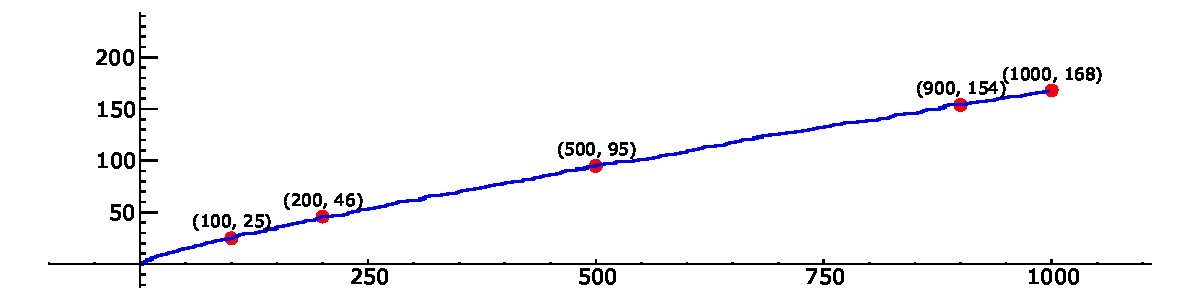
\includegraphics[width=\textwidth]{graphics/prime_pi}
\caption{Graph of $\pi(x)$ for $x<1000$}\label{fig:pix}
\end{figure}

Gauss\index{Gauss} was an inveterate computer:
he wrote in an 1849 letter that there are
$216,745$ primes less than $3,000,000$ (this is wrong but close;
the correct count is $216,816$).

Gauss conjectured the following asymptotic formula for $\pi(x)$, which was
later proved independently by Hadamard\index{Hadamard} and Vall\'ee
Poussin\index{Vall\'ee Poussin} in 1896 (but will not be proved in
this book).
\begin{theorem}[Prime Number Theorem]\label{thm:primenumber}
\ithm{prime number}
The function $\pi(x)$ is asymptotic to $x/\log(x)$, in the sense that
   $$\lim_{x\ra \infty}  \frac{\pi(x)}{ x/\log(x)} = 1.$$
\end{theorem}
We do nothing more here than motivate this deep theorem with
a few further observations.
The theorem implies that
$$\lim_{x\ra \infty} \frac{\pi(x)}{x}  = \lim_{x\ra \infty} \frac{1}{\log(x)} =0,$$
so for any~$a$,
$$\lim_{x\ra\infty} \frac{\pi(x)}{x/(\log(x)-a)} =
    \lim_{x\ra\infty} \frac{\pi(x)}{x/\log(x)} - \frac{a\pi(x)}{x}
          = 1.$$
Thus $x/(\log(x)-a)$ is also asymptotic to $\pi(x)$ for
any~$a$.  See \cite[\S1.1.5]{primenumbers} for a discussion of why
$a=1$ is the best choice.  Table~\ref{tab:pnt} compares
$\pi(x)$ and $x/(\log(x)-1)$ for several $x<10000$.

\begin{table}\index{table!comparing $\pi(x)$ to $x/(\log(x)-1)$}
%? pi(x, c=0) = forprime(p=2,x,c++); c;
%? for(n=1,10,print(n*1000,"\t",pi(n*1000),"\t",n*1000/(log(n*1000)-1)))
\caption{Comparison of $\pi(x)$ and $x/(\log(x)-1)$\label{tab:pnt}}\vspace{1ex}

\begin{center}
\begin{tabular}{|l|l|l|}\hline
$\quad{}\!x$& $\pi(x)$ & $x/(\log(x)-1)$ (approx)\\\hline
1000&   168&    169.2690290604408165186256278\\
2000&   303&    302.9888734545463878029800994\\
3000&   430&    428.1819317975237043747385740\\
4000&   550&    548.3922097278253264133400985\\
5000&   669&    665.1418784486502172369455815\\
6000&   783&    779.2698885854778626863677374\\
7000&   900&    891.3035657223339974352567759\\
8000&   1007&   1001.602962794770080754784281\\
9000&   1117&   1110.428422963188172310675011\\
10000&  1229&   1217.976301461550279200775705\\\hline
\end{tabular}
\end{center}
\end{table}

\begin{figure}
\begin{center}
\vspace{2ex}
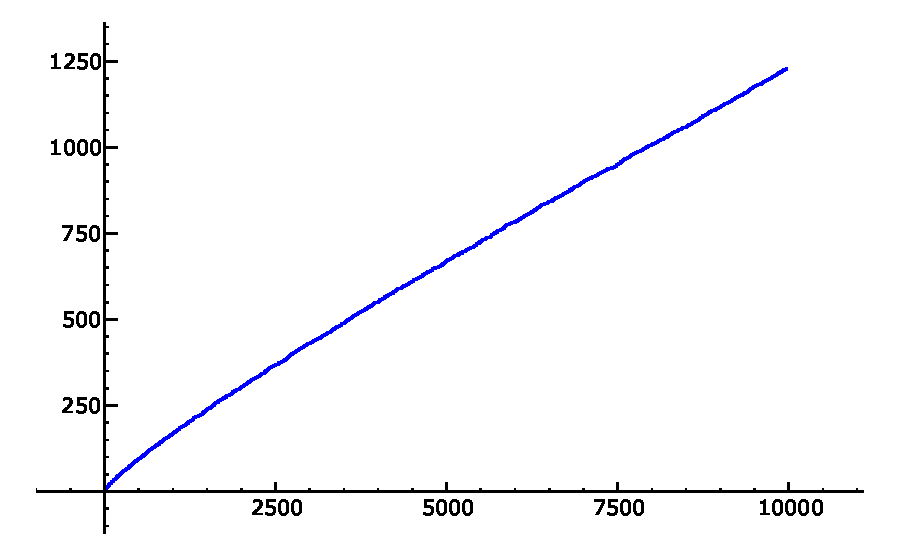
\includegraphics[width=0.45\textwidth]{graphics/prime_pi_10000}
\vspace{4ex}
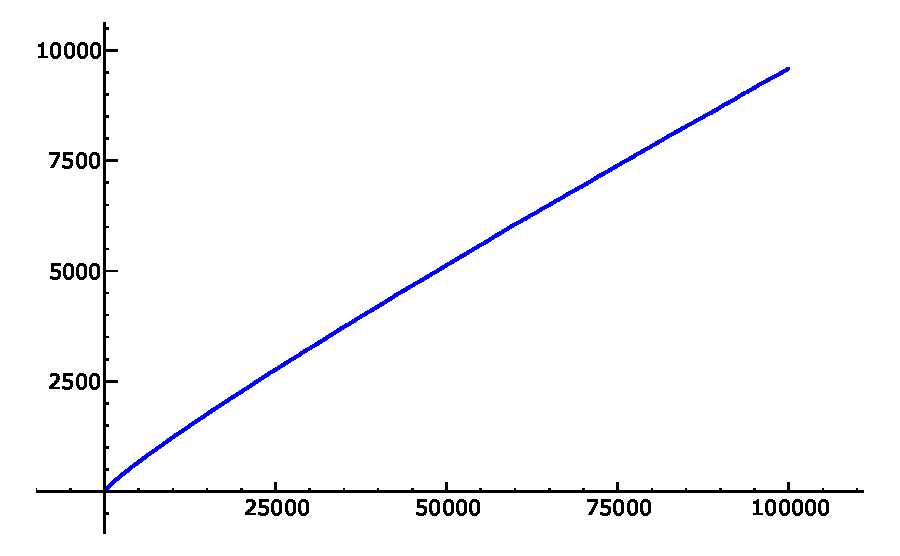
\includegraphics[width=0.45\textwidth]{graphics/prime_pi_100000}
\caption{Graphs of $\pi(x)$ for $x<10000$ and $x<100000$\label{fig:pix2}}
\end{center}
\end{figure}

The record for counting primes is\index{largest known!value of $\pi(x)$}
$$
  \pi(10^{23}) = 1925320391606803968923.
  $$
  Note that such computations are very difficult to get exactly right,
  so the above might be slightly wrong.

For the reader familiar with complex analysis, we mention a connection
between $\pi(x)$ and the Riemann Hypothesis.  The Riemann zeta
function $\zeta(s)$ is a complex analytic function on $\C\setminus
\{1\}$ that extends the function defined on a right half plane by
$\sum_{n=1}^{\infty} n^{-s}$.  The Riemann Hypothesis\index{Riemann
  Hypothesis} is the conjecture that the zeros in $\C$ of $\zeta(s)$
with positive real part lie on the line ${\rm Re}(s)=1/2$. This
conjecture is one of the Clay Math Institute million dollar millennium
prize problems \cite{cmi}.

  According to \cite[\S1.4.1]{primenumbers}, the Riemann Hypothesis is
  equivalent to the conjecture that
$$
  \Li(x) = \int_{2}^{x} \frac{1}{\log(t)} dt
$$
is a ``good'' approximation to $\pi(x)$, in the following
precise sense.
\begin{conjecture}[Equivalent to the Riemann Hypothesis]
\index{Riemann Hypothesis!bound on $\pi(x)$}
\mbox{}\newline{}For all  $x\geq 2.01$,
$$
 |\pi(x)-\Li(x)| \leq \sqrt{x}\log(x).
$$
\end{conjecture}
If $x=2$, then $\pi(2)=1$ and $\Li(2)=0$,
but $\sqrt{2}\log(2) = 0.9802\ldots$, so the inequality
is not true for $x\geq 2$, but $2.01$ is big enough.
We will do nothing more to explain this conjecture,
and settle for one numerical example.
\begin{example}
Let $x=4\cdot 10^{22}$.  Then
\begin{align*}
  \pi(x) &= 783964159847056303858,\\
  \Li(x) &= 783964159852157952242.7155276025801473\ldots, \\
  |\pi(x) - \Li(x)| &= 5101648384.71552760258014\ldots, \\
  \sqrt{x}\log(x) &=  10408633281397.77913344605\ldots, \\
  x/(\log(x)-1)  &=  783650443647303761503.5237113087392967\ldots.
\end{align*}
\end{example}


\begin{sg}
We use \sage to graph $\pi(x)$, $\Li(x)$, and $\sqrt{x}\log(x)$.
\begin{verbatim}
sage: P = plot(Li, 2,10000, rgbcolor='purple')
sage: Q = plot(prime_pi, 2,10000, rgbcolor='black')
sage: R = plot(sqrt(x)*log(x),2,10000,rgbcolor='red')
sage: show(P+Q+R,xmin=0, figsize=[8,3])
\end{verbatim}
\begin{center}
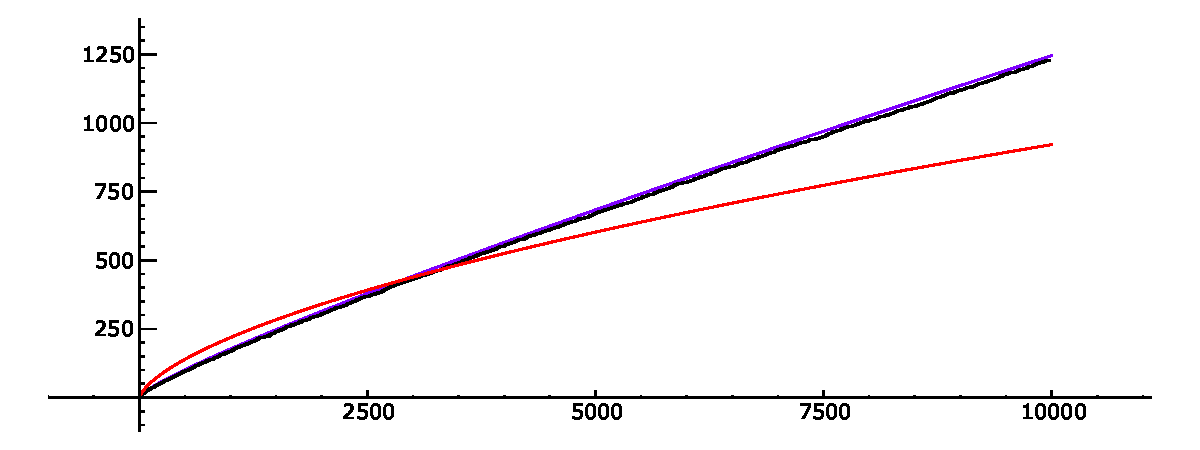
\includegraphics[width=\textwidth]{graphics/rh}
\end{center}
The topmost line is $\Li(x)$, the next line is $\pi(x)$, and the
bottom line is $\sqrt{x}\log(x)$.
\end{sg}

For more on the prime number theorem and
the Riemann hypothesis see \cite{zagier:primes50}
and \cite{mazur-stein:rh}.

\begin{exercises}

\item Compute the greatest common divisor $\gcd(455,1235)$ by hand.

\item\label{ex:handsieve} Use the prime enumeration sieve
to make a list of all primes up to $100$.

\item\label{ex:primesform} Prove that there are infinitely
many primes of the form $6x-1$.\index{primes!of the form $6x-1$}

\item \label{ex:fewprimes}
Use Theorem~\ref{thm:primenumber} to deduce that
$\ds \lim_{x\to\infty} \frac{\pi(x)}{x} = 0$.

\item Let $\psi(x)$ be the number of primes of the form
$4k-1$ that are $\leq x$.  Use a computer to make a conjectural
guess about $\lim_{x\to\infty} \psi(x) / \pi(x)$.

\item So far $44$ Mersenne primes $2^p-1$ have been discovered.
Give a guess, backed up by an argument, about
when the next Mersenne prime might be discovered (you will have
to do some online research).

\item
 \begin{enumerate}
\item Let $y=10000$.  Compute
  $\pi(y) = \#\{ \text{primes } p \leq y\}.$
\item The prime number theorem implies $\pi(x)$ is
asymptotic to $\frac{x}{\log(x)}$.  How close is $\pi(y)$ to
$y/\log(y)$, where $y$ is as in (a)?
\end{enumerate}

\item Let $a,b,c,n$ be integers.  Prove that
\begin{enumerate}
\item if $a \mid n$ and $b\mid n$ with $\gcd(a,b)=1$, then $ab\mid n$.
\item if $a\mid bc$ and $\gcd(a,b)=1$, then $a\mid c$.
\end{enumerate}

\item Let $a,b,c,d$, and $m$ be integers.  Prove that
\begin{enumerate}
\item if $a\mid b$ and $b\mid c$ then $a\mid c$. %Jones&Jones
\item if $a\mid b$ and $c\mid d$ then $ac\mid bd$.
\item if $m\neq 0$, then $a\mid b$ if and only if $ma\mid mb$.
\item if $d\mid a$ and $a\neq 0$, then $|d|\leq |a|$.
\end{enumerate}

% pg 13 of kumanduri/romero
\item
In each of the following, apply the division algorithm
to find $q$ and $r$ such that
$a = bq + r$ and $0\leq r < |b|$:
$$
 a=300, b=17,\,\,
a=729,b=31,\,\,
a=300,b=-17,\,\,
a=389,b=4.
$$

\item
\begin{enumerate}
\item (Do this part  by hand.) Compute the greatest common
  divisor of $323$ and $437$ using the algorithm described in class
  that involves quotients and remainders (i.e., do not just factor $a$
  and $b$).
\item Compute by any means the greatest common divisor of
$$314159265358979323846264338$$ and $$271828182845904523536028747.$$
\end{enumerate}

\item
\begin{enumerate}
\item Suppose $a$, $b$ and $n$ are positive integers. Prove
that if $a^n\mid b^n$, then $a\mid b$.
\item Suppose $p$ is a prime and $a$ and $k$ are positive
integers.  Prove that if $p \mid a^k$, then $p^k \mid a^k$.
\end{enumerate}

%Burton, page 26
\item
\begin{enumerate}
\item  Prove that if a positive integer $n$ is a perfect
square, then $n$ cannot be written in the form $4k+3$
for $k$ an integer.
(Hint: Compute the remainder upon division
by $4$ of each of $(4m)^2$, $(4m+1)^2$, $(4m+2)^2$,
and $(4m+3)^2$.)
\item  Prove that no integer in the sequence
$$
  11, 111, 1111, 11111, 111111, \ldots
$$
is a perfect square.   (Hint: $111\cdots111 = 111\cdots 108 + 3 = 4k+3$.)
\end{enumerate}

\item Prove that a positive integer $n$ is prime if
and only if $n$ is not divisible by any prime $p$
with $1 < p \leq \sqrt{n}$.


\end{exercises}
%%%%%%%%%%%%%%%%%%%%%%%%%%%%%%%%%%%%%%%%%%%%%%%%%%%%%%%%%%%%%%%%%%%%%%%
%%
%% Chapter: Integers Modulo n
%%
%%%%%%%%%%%%%%%%%%%%%%%%%%%%%%%%%%%%%%%%%%%%%%%%%%%%%%%%%%%%%%%%%%%%%%%

\chapter{The Ring of Integers Modulo {\em n}}\label{ch:cong}
A startling fact about numbers is that it takes less than a second to
decide with near certainty whether or not any given 1,000 digit number
$n$ is a prime, {\em without actually factoring~$n$}.  The algorithm
for this involves doing some arithmetic with $n$ that works
differently depending on whether $n$ is prime or composite.  In
particular, we do arithmetic with the set (in fact, ``ring'') of
integers $\{0,1,\ldots, n-1\}$ using an innovative rule for addition
and multiplication, where the sum and product of two elements of that
set is again in that set.
%Though completely solving the problem of
%recognizing primes requires sophisticated techniques that will not be
%completely explained in this chapter, we will explain several of the
%key ideas.

Another surprising fact is that one can almost instantly compute the
last 1,000 digits of a massive multi-billion digit number like $n =
1234^{1234567890}$ without explicitly writing down all the digits of
$n$.  Again, this calculation involves arithmetic with the ring
$\{0,1,\ldots, n-1\}$.

This chapter is about the ring $\zmod{n}$ of integers modulo~$n$, the
beautiful structure this ring has, and how to apply it to the above
mentioned problems, among others.\index{$\zmod{n}$} It is foundational
for the rest of this book. In Section~\ref{sec:congruences}, we discuss
when linear equations modulo~$n$ have a solution, then introduce the
Euler~$\vphi$ function and prove Euler's Theorem and Wilson's theorem.
In Section~\ref{sec:chinese}, we prove the Chinese Remainer
Theorem, which addresses simultaneous solubility of several linear
equations modulo coprime moduli.  With these theoretical foundations
in place, in Section~\ref{sec:arith_mod_n}, we introduce algorithms for
doing powerful computations modulo~$n$, including computing large
powers quickly, and solving linear equations.  We finish in
Section~\ref{sec:prob_prime_test} with a discussion of recognizing
prime numbers using arithmetic modulo~$n$.

% We assume the reader has read Chapter~\ref{ch:prime}, and knows what
% it means to take the quotient of the ring $\Z$ by an ideal $n\Z$.

\section{Congruences Modulo $n$}\index{congruences}
\index{equivalence relation!congruence modulo~$n$}
\index{integers!modulo~$n$}
\label{sec:congruences}

\begin{definition}[Group]\label{defn:group}\index{group}\index{group!of units}\index{unit group}
A {\em group} is a set $G$ equipped with a binary operation
$G \times G \to G$ (denoted by multiplication below)
and an identity element $1\in G$ such that:
\begin{enumerate}
\item For all $a,b,c\in G$, we have $(ab)c = a(bc)$.
\item For each $a\in G$, we have $1a=a1=a$, and there exists $b\in G$ such that
$ab = 1$.
\end{enumerate}
\end{definition}

\begin{definition}[Abelian Group]\label{defn:abelian}
An \defn{abelian group} is a group $G$
such that $ab=ba$ for every $a,b\in G$.
\end{definition}


\begin{definition}[Ring]\label{defn:ring}
A \defn{ring} $R$ is a set equipped with binary operations
$+$ and $\times$ and elements $0,1\in R$ such that
$R$ is an abelian group under $+$,
and for all $a,b,c \in R$ we have
\begin{itemize}
\item $1a = a1 = a$
\item $(ab)c = a(bc)$
\item $a(b+c) = ab + ac$.
\end{itemize}
If, in addition, $ab=ba$ for all $a,b\in R$, then we
call $R$ a \defn{commutative ring}.
\end{definition}

In this section, we define the ring $\zmod{n}$ of integers modulo~$n$,
introduce the Euler $\vphi$-function,\index{Euler!phi function}
\index{phi@$\vphi$ function} and relate it to the multiplicative
order\index{multiplicative!order} of certain elements of $\zmod{n}$.

If $a,b\in\Z$ and $n\in\N$, we say that $a$ is {\em congruent to~$b$
  modulo~$n$} if $n\mid a-b$, and write $a\con b\pmod{n}$.  Let
$n\Z=(n)$ be the subset of $\Z$ consisting of all multiples of $n$
(this is called the ``ideal of $\Z$ generated by~$n$'').
\begin{definition}[Integers Modulo $n$]
  The ring $\zmod{n}$ of \defn{integers modulo~$n$} is the set of
  equivalence classes of integers modulo~$n$.  It is equipped with its
  natural ring structure:
$$
  (a + n\Z) + (b + n\Z) = (a+b) + n\Z
$$
$$
  (a + n\Z) \cdot (b + n\Z) = (a\cdot b) + n\Z.
$$
\end{definition}


\begin{example}
For example,
$$
  \zmod{3} = \{ \{\ldots, -3, 0, 3, \ldots\},
              \{\ldots, -2, 1, 4, \ldots\},
              \{\ldots, -1, 2, 5, \ldots\}\}
$$
\begin{sg}
In \sage, we list the elements of $\Z/n\Z$ as follows:
\begin{verbatim}
sage: R = Integers(3)
sage: list(R)
[0, 1, 2]
\end{verbatim}
\end{sg}
\end{example}

\label{page:znring}
We use the notation $\zmod{n}$ because $\zmod{n}$ is the quotient of
the ring~$\Z$ by the ``ideal'' $n\Z$ of multiples of~$n$.  Because
$\zmod{n}$ is the quotient of a ring by an ideal, the ring structure
on~$\Z$ induces a ring structure on $\zmod{n}$.
We often let~$a$ or $a\pmod{n}$
denote the equivalence class $a+n\Z$ of~$a$.

\begin{definition}[Field]\label{defn:field}
A \defn{field} $K$ is a ring such that for every
nonzero element $a\in K$ there is an element $b\in K$
such that $ab=1$.
\end{definition}

For example, if~$p$ is a prime, then $\zmod{p}$ is a
field\index{field!of integers modulo $p$} (see
\exref{ch:cong}{ex:zpfield}).\index{finite field}

\begin{definition}[Reduction Map and Lift]
  We call the natural reduction map $\Z \to \zmod{n}$, which sends $a$
  to $a+n\Z$, \defn{reduction modulo~$n$}.  We also say that $a$ is a
  \defn{lift} of $a+n\Z$.  Thus, e.g., $7$ is a lift of $1$ mod $3$,
  since $7+3\Z = 1+3\Z$.
\end{definition}

We can use that arithmetic in $\zmod{n}$ is well defined is to
derive tests for divisibility\index{divisibility tests} by $n$ (see
\exref{ch:cong}{ex:divrules}).
\begin{proposition}\label{prop:div3}\iprop{divisibility by 3}
A number $n\in\Z$ is divisible by~$3$ if and only if
the sum of the digits of~$n$ is divisible by~$3$.
\end{proposition}
\begin{proof}
Write
 $$n=a+10b+100c+\cdots,$$
where the digits of~$n$ are $a$, $b$, $c$, etc.
Since $10\con 1\pmod{3}$,
$$
  n = a + 10b + 100c+\cdots \con a + b + c+\cdots \pmod{3},
$$
from which the proposition follows.
\end{proof}


\subsection{Linear Equations Modulo~$n$}\label{sec:lineq}\index{linear equations modulo $n$}%
\index{modular arithmetic!and linear equations} In this section, we
are concerned with how to decide whether or not a linear equation of
the form $ax\con b \pmod{n}$ has a solution modulo~$n$.
Algorithms for {\em computing} solutions to $ax\con
b\pmod{n}$ are the topic of Section~\ref{sec:arith_mod_n}.

First, we prove a proposition that gives a criterion under
which one can cancel a quantity from both sides of a congruence.
\begin{proposition}[Cancellation]\label{prop:cancel}\iprop{cancellation}
If $\gcd(c,n)=1$ and
$$
   ac\con bc\pmod{n},
$$
then $a \con b\pmod{n}$.
\end{proposition}
\begin{proof}
By definition
$$
  n \mid ac - bc = (a-b)c.
$$
Since $\gcd(n,c)=1$, it follows
from Theorem~\ref{thm:fundamental} that $n\mid a-b$, so
$$
   a \con b\pmod{n},
$$
as claimed.
\end{proof}



When~$a$ has a multiplicative inverse $a'$ in $\zmod{n}$ (i.e.,
$aa'\con 1\pmod{n}$) then the equation $ax\con b\pmod{n}$ has a unique
solution $x\con a'b\pmod{n}$.  Thus, it is of interest to
determine the units in $\zmod{n}$, i.e., the elements which have a
multiplicative inverse.

We will use complete sets of residues\index{complete set of residues}
to prove that the units in $\zmod{n}$ are exactly the~$a\in\zmod{n}$
such that $\gcd(\tilde{a},n)=1$ for any lift $\tilde{a}$ of~$a$
to~$\Z$ (it doesn't matter which lift).

\begin{definition}[Complete Set of Residues]
We call a subset $R\subset\Z$ of size~$n$ whose reductions modulo~$n$ are
pairwise distinct a \defn{complete set of residues}
modulo~$n$.  In other words, a complete set of residues is a choice of
representative for each equivalence class in $\zmod{n}$.
\end{definition}
For example,
$$
   R=\{0,1,2,\ldots,n-1\}
$$
is a complete set of residues modulo~$n$.
When $n=5$,
$R = \{0,1,-1,2,-2\}$
is a complete set of residues.

\begin{lemma}\label{lem:residues}
If~$R$ is a complete set of residues modulo~$n$ and $a\in\Z$ with
$\gcd(a,n)=1$, then $aR = \{ax : x \in R\}$
is also a complete set of residues modulo~$n$.
\end{lemma}
\begin{proof}
If $ax\con ax'\pmod{n}$ with $x, x'\in R$, then
Proposition~\ref{prop:cancel} implies that $x\con{}x'\pmod{n}$.
Because $R$ is a complete set of residues, this implies
that $x=x'$.  Thus the elements of
$aR$ have distinct reductions modulo~$n$.
It follows, since $\#aR=n$, that $aR$ is a
complete set of residues modulo~$n$.
\end{proof}

\begin{proposition}[Units]\label{prop:unitsmodn}\iprop{units}
If $\gcd(a,n)=1$, then the equation
$
 ax\con b\pmod{n}
$
has a solution, and that solution is unique modulo~$n$.
\end{proposition}
\begin{proof}
Let~$R$ be a complete set of residues modulo~$n$, so there
is a unique element of~$R$ that is congruent to~$b$ modulo~$n$.
By Lemma~\ref{lem:residues},
$aR$ is also a complete set of residues modulo~$n$, so
there is a unique element $ax\in aR$ that is congruent
to~$b$ modulo~$n$, and we have $ax\con b\pmod{n}$.
\end{proof}
Algebraically, this proposition asserts that if $\gcd(a,n)=1$, then
the map $\zmod{n}\ra \zmod{n}$ given by left multiplication by~$a$ is
a bijection.

\begin{example}
Consider the equation $2x\con 3\pmod{7}$,
and the complete set $R = \{0,1,2,3,4,5,6\}$
of coset representatives.  We have
$$
  2R = \{0,2,4,6,8\con 1, 10\con 3, 12\con 5\},
$$
so $2\cdot 5\con 3\pmod{7}$.
\end{example}

When $\gcd(a,n)\neq 1$, then the equation $ax\con b\pmod{n}$ may or
may not have a solution.  For example, $2x\con 1\pmod{4}$ has no
solution, but $2x\con 2\pmod{4}$ does, and in fact it has more than
one mod~$4$ ($x=1$ and $x=3$).  Generalizing
Proposition~\ref{prop:unitsmodn}, we obtain the following more general
criterion for solvability.
\begin{proposition}[Solvability]\label{prop:cancel2}\iprop{solvability}
The equation $ax\con b\pmod{n}$ has a solution
if and only if $\gcd(a,n)$ divides~$b$.
\end{proposition}
\begin{proof}
  Let $g=\gcd(a,n)$.  If there is a solution~$x$ to the equation
  $ax\con b\pmod{n}$, then $n\mid (ax-b)$.  Since $g\mid n$ and $g\mid
  a$, it follows that $g\mid b$.

  Conversely, suppose that $g\mid b$.  Then $n\mid (ax-b)$ if and only
  if $$
  \frac{n}{g} \mid \left(\frac{a}{g} x - \frac{b}{g}\right).  $$
  Thus $ax\con b\pmod{n}$ has a solution if and only if $\frac{a}{g}x
  \con \frac{b}{g}\pmod{\frac{n}{g}}$ has a solution.  Since
  $\gcd(a/g, n/g)=1$, Proposition~\ref{prop:unitsmodn} implies this
  latter equation does have a solution.
\end{proof}

In Chapter~\ref{ch:reciprocity}, we will study quadratic reciprocity,
which gives a nice criterion for whether or not a quadratic equation
modulo~$n$ has a solution.

\subsection{Euler's Theorem}
\index{Euler's theorem}%
\label{sec:flittle}%
\index{theorem!Euler's}%
Let $(\zmod{n})^*$ denote the set of elements $[x] \in \zmod{n}$
such that $\gcd(x,n)=1$.

The set $(\zmod{n})^*$ is a group, called the {\em group of units of
  the ring $\zmod{n}$}; it will be of great interest to us.  Each
element of this group has an order, and Lagrange's theorem from group
theory implies that each element of $(\zmod{n})^*$ has an order that
divides the order of $(\zmod{n})^*$.  In elementary number theory, this
fact goes by the monicker ``Fermat's Little Theorem'' when $n$ is
prime and ``Euler's Theorem'' in general, and we reprove it from basic
principles in this section.

\begin{definition}[Order of an Element]\index{order!of element}%
\index{modular arithmetic!order of element}\label{defn:order}
Let $n\in\N$ and $x\in\Z$ and suppose that $\gcd(x,n)=1$.
The \defn{order} of $x$ modulo~$n$ is the smallest $m\in\N$
such that
$$
  x^m \con 1\pmod{n}.
$$
\end{definition}
To show that the definition makes sense, we verify
that such an~$m$ exists.  Consider $x, x^2, x^3, \ldots$ modulo~$n$.
There are only finitely many residue classes modulo~$n$, so we must
eventually find two integers $i, j$ with $i<j$ such that
$$
  x^j\con x^i\pmod{n}.
$$
Since $\gcd(x,n)=1$, Proposition~\ref{prop:cancel} implies that
we can cancel~$x$'s and conclude that
$$
  x^{j-i}\con 1\pmod{n}.
$$

\begin{sg}
Use \code{x.multiplicative\_order()} to compute the
order of an element of $\Z/n\Z$ in \sage.
\begin{verbatim}
sage: R = Integers(10)
sage: a = R(3)                 # create an element of Z/10Z
sage: a.multiplicative_order()
4
\end{verbatim}%link
Notice that the powers of $a$ are periodic with period $4$, i.e.,
there are four powers and they repeat:
%link
\begin{verbatim}
sage: [a^i for i in range(15)]
[1, 3, 9, 7, 1, 3, 9, 7, 1, 3, 9, 7, 1, 3, 9]
\end{verbatim}
The command \code{range(n)} we use
above returns the list of integers between $0$ and $n-1$,
inclusive.
\end{sg}


\begin{definition}[Euler's $\vphi$-function]\label{def:phi}\index{Euler!phi function}
For $n\in\N$, let
$$
 \vphi(n) = \#\{a \in \N : a \leq n \text{ and } \gcd(a,n)=1\}.
$$
\end{definition}
For example,
\begin{align*}
 \vphi(1) &= \#\{1\} = 1,\\
 \vphi(2) &= \#\{1\} = 1,\\
 \vphi(5) &= \#\{1,2,3,4\} = 4,\\
 \vphi(12) &= \#\{1,5,7,11\} = 4.\\
\end{align*}
Also, if~$p$ is any prime number then
$$
   \vphi(p) = \#\{1,2,\ldots,p-1\} = p-1.
$$
In Section~\ref{sec:multi_funcs}, we prove
that if $\gcd(m,r)=1$, then $\vphi(mr)=\vphi(m)\vphi(r).$  This will
yield an easy way to compute $\vphi(n)$ in terms of the prime
factorization of~$n$.
\begin{sg}
Use the \code{euler\_phi(n)} command to compute $\vphi(n)$
in \sage:
\begin{verbatim}
sage: euler_phi(2007)
1332
\end{verbatim}
\end{sg}

\begin{theorem}[Euler's Theorem]\label{thm:fermatlittle}
\ithm{Euler's}
If $\gcd(x,n)=1$, then
$$
   x^{\vphi(n)} \con 1\pmod{n}.
$$
\end{theorem}
\begin{proof}
As mentioned above, Euler's Theorem has the following group-theoretic
\index{Euler's theorem!group-theoretic interpretation}
interpretation.  The set of units in $\zmod{n}$ is a group
\index{group!$(\zmod{m})^*$}
$$
(\zmod{n})^*
= \{ a \in \zmod{n} : \gcd(a,n) = 1\}
$$
that has order~$\vphi(n)$.  The theorem then asserts
that the order of an element of $(\zmod{n})^*$ divides the order
$\vphi(n)$ of $(\zmod{n})^*$.   This is a special case of the more
general fact (Lagrange's Theorem) that if~$G$ is a finite group and
$g\in G$, then the order of~$g$ divides the cardinality of~$G$.

We now give an elementary proof of the theorem.  Let
$$
  P = \{ a : 1\leq a \leq n \text{ and } \gcd(a,n) = 1\}.
$$
In the same way that we proved Lemma~\ref{lem:residues},
we see that the reductions modulo~$n$ of the elements of $xP$
are the same as the reductions of the elements of $P$.
Thus
$$
 \prod_{a\in P} (xa) \con \prod_{a \in P} a \pmod{n},
$$
since the products are over the same numbers modulo~$n$.
Now cancel the $a$'s on both sides to get
$$x^{\#P} \con 1\pmod{n},$$
as claimed.
\end{proof}

\begin{sg}
We illustrate Euler's Theorem using \sage.
The \code{Mod(x,n)} command  returns the equivalence
class of $x$ in $\Z/n\Z$.
\begin{verbatim}
sage: n = 20
sage: k = euler_phi(n); k
8
sage: [Mod(x,n)^k for x in range(n) if gcd(x,n) == 1]
[1, 1, 1, 1, 1, 1, 1, 1]
\end{verbatim}
\end{sg}


\subsection{Wilson's Theorem}\index{Wilson's theorem}\index{theorem!of Wilson}
The following characterization of prime numbers, from the 1770s, is
called ``Wilson's Theorem,'' though it was first proved by
Lagrange\index{Lagrange}.
\begin{proposition}[Wilson's Theorem]\label{prop:wilson}\iprop{Wilson}
An integer $p>1$ is prime if and only if
$(p-1)! \con -1 \pmod{p}.$
\end{proposition}
For example,
if $p=3$, then $(p-1)! = 2\con -1\pmod{3}$.
If $p=17$, then
$$(p-1)! = 20922789888000 \con -1\pmod{17}.$$
But if $p=15$, then
$$(p-1)! = 87178291200 \con 0 \pmod{15},$$
so $15$ is composite.  Thus Wilson's theorem could be viewed
as a primality test, though, from a computational point of view,
it is probably one of the world's {\em least efficient}
primality tests since computing $(n-1)!$ takes so many steps.
\begin{proof}
The statement is clear when $p=2$, so henceforth we assume
that $p>2$.
We first assume that~$p$ is prime and prove that
$(p-1)! \con -1\pmod{p}$.  If $a\in\{1,2,\ldots,p-1\}$, then
the equation
$$
  ax\con 1\pmod{p}
$$
has a unique solution $a'\in\{1,2,\ldots,p-1\}$.
If $a=a'$, then $a^2\con 1\pmod{p}$, so
$p\mid a^2-1 = (a-1)(a+1)$, so
$p\mid (a-1)$ or $p\mid (a+1)$, so $a\in\{1,p-1\}$.
We can thus pair off the elements of
$\{2,3,\ldots,p-2\}$,
each with their inverse.
Thus
$$
  2\cdot 3 \cdot \cdots \cdot (p-2) \con 1\pmod{p}.
$$
Multiplying both sides by $p-1$ proves that
$(p-1)! \con -1\pmod{p}$.

Next, we assume that $(p-1)! \con -1\pmod{p}$ and
prove that~$p$ must be prime.  Suppose not, so that~$p\geq 4$
is a composite number.  Let~$\ell$ be a prime divisor
of~$p$.  Then $\ell<p$, so $\ell\mid (p-1)!$.  Also,
by assumption,
$$
  \ell \mid p \mid ((p-1)! + 1).
$$
This is a contradiction, because a prime can not divide a number~$a$ and
also divide $a+1$, since it would then have to divide $(a+1) - a=1$.
\end{proof}

\begin{example}
We illustrate the key step in the above proof in the case $p=17$.
We have
$$
2\cdot 3 \cdots  15
  = (2\cdot 9)\cdot(3\cdot 6)\cdot(4\cdot 13)\cdot
    (5\cdot 7)\cdot(8\cdot 15)\cdot(10\cdot 12)\cdot(14\cdot 11)
  \con 1\pmod{17},$$
where we have paired up the numbers $a, b$ for
which $ab\con 1\pmod{17}$.
\end{example}

\begin{sg}
  We use \sage to create a table of triples; the first column contains
  $n$, the second column contains $(n-1)!$ modulo $n$, and the third
  contains $-1$ modulo $n$.  Notice that the first columns contains a
  prime precisely when the second and third columns are equal.  (The
  ... notation indicates a multi-line command in \sage; you should not
  type the dots in explicitly.)
\begin{verbatim}
sage: for n in range(1,10):
...    print n, factorial(n-1) % n, -1 % n
1 0 0
2 1 1
3 2 2
4 2 3
5 4 4
6 0 5
7 6 6
8 0 7
9 0 8
\end{verbatim}
\end{sg}

\section{The Chinese Remainder Theorem}\label{sec:chinese}%
\index{Chinese remainder theorem}
In this section, we prove the Chinese Remainder Theorem, which gives
conditions under which a system of linear equations is guaranteed to
have a solution.
In the 4th century a Chinese mathematician asked the following:
\begin{question}\label{q:chinese}
There is a quantity whose number is unknown. Repeatedly divided
by 3, the remainder is 2; by 5 the remainder is 3; and by 7 the
remainder is 2. What is the quantity?
\end{question}
In modern notation, Question~\ref{q:chinese}  asks us to
find a positive integer solution to the following system of
three equations:
\begin{align*}
x &\con 2 \pmod{3}\\
x &\con 3 \pmod{5}\\
x &\con 2 \pmod{7}
\end{align*}
The Chinese Remainder Theorem asserts that a solution
exists, and the proof gives a method to find one.
(See Section~\ref{sec:arith_mod_n} for the necessary algorithms.)


\begin{theorem}[Chinese Remainder Theorem]\label{thm:crt}%
\ithm{Chinese remainder}
Let $a, b\in\Z$ and $n,m\in\N$ such that
$\gcd(n,m)=1$.  Then there exists $x\in\Z$ such that
\begin{align*}
x&\con a\pmod{m},\\
x&\con b\pmod{n}.
\end{align*}
Moreover~$x$ is unique modulo~$mn$.
\end{theorem}
\begin{proof}
If we can solve for~$t$ in the equation
$$
   a+tm \con b \pmod{n},
$$
then $x=a+tm$ will satisfy both congruences.
To see that we can solve, subtract~$a$ from
both sides and use Proposition~\ref{prop:unitsmodn}
together with our assumption that $\gcd(n,m)=1$  to see that
there is a solution.

For uniqueness, suppose that $x$ and $y$ solve both congruences.  Then
$z=x-y$ satisfies $z\con 0\pmod{m}$ and $z\con 0\pmod{n}$, so $m\mid
z$ and $n\mid z$.  Since $\gcd(n,m)=1$, it follows that $nm\mid z$, so
$x\con y\pmod{nm}$.
\end{proof}

% An alternative approach to proving Theorem~\ref{thm:crt} is to prove
% the result for the special cases $a=1,b=0$ and for $a=0,b=1$, then
% take a suitable linear combination of those two solutions.  This is
% geometrically appealing, since it is like writing a vector in terms of
% a basis.

\begin{algorithm}{Chinese Remainder Theorem}\label{alg:crt}
Given coprime integers $m$ and $n$ and integers $a$ and $b$,
this algorithm find an integer $x$ such that $x\con a\pmod{m}$
and $x\con b\pmod{n}$.
\begin{steps}
\item{}[Extended GCD] Use Algorithm~\ref{alg:xgcd} below
to find integers $c,d$ such that $cm+dn=1$.
\item{}[Answer] Output $x =a + (b-a)cm$ and terminate.
\end{steps}
\end{algorithm}
\begin{proof}
Since $c\in\Z$, we have $x\con a\pmod{m}$,
and using that $cm+dn=1$,  we have
$a + (b-a)cm \con a + (b-a) \con b\pmod{n}$.
\end{proof}

Now we can answer Question~\ref{q:chinese}.
First, we use Theorem~\ref{thm:crt}
to find a solution to the pair of equations
\begin{align*}
x &\con 2 \pmod{3},\\
x &\con 3 \pmod{5}.
\end{align*}
Set $a=2$, $b=3$, $m=3$, $n=5$.
Step 1 is to find a solution to $t\cdot 3 \con 3-2\pmod{5}$.
A solution is $t=2$.  Then $x=a+tm=2+2\cdot 3 = 8$.
Since any~$x'$ with $x'\con x\pmod{15}$ is also a solution to
those two equations, we can solve all three equations by
finding a solution to the pair of equations
\begin{align*}
x &\con 8 \pmod{15}\\
x &\con 2 \pmod{7}.
\end{align*}
Again, we find a solution to $t\cdot 15 \con 2-8\pmod{7}$.
A solution is $t = 1$, so
$$x=a+tm=8+15=23.$$
Note that there are other solutions.  Any $x'\con x\pmod{3\cdot 5\cdot 7}$
is also a solution; e.g., $23+3\cdot 5\cdot 7 = 128$.

\begin{sg}
The \code{CRT(a,b,m,n)} command in Sage computes an integer $x$
such that $x\con a\pmod{m}$ and $x\con b\pmod{n}$.  For example,
\begin{verbatim}
sage: CRT(2,3, 3, 5)
8
\end{verbatim}
\noindent{}The \code{CRT\_list} command computes a number that reduces to
several numbers modulo coprime moduli.  We use
it to answer Question~\ref{q:chinese}:
\begin{verbatim}
sage: CRT_list([2,3,2], [3,5,7])
23
\end{verbatim}
\end{sg}

\subsection{Multiplicative Functions}\index{multiplicative!functions}%
\label{sec:multi_funcs}%
Recall from Definition~\ref{def:phi}
that the \defn{Euler $\vphi$-function}\index{Euler!phi function} is
$$
  \vphi(n) = \#\{a : 1\leq a \leq n\text{ and }\gcd(a,n)=1\}.
$$

\begin{lemma}\label{lem:units_map}
Suppose that $m,n\in\N$ and $\gcd(m,n)=1$.
Then the map
\begin{equation}\label{eqn:crtprod}
\psi: (\zmod{mn})^* \ra (\zmod{m})^* \cross (\zmod{n})^*.
\end{equation}
defined by
$$
 \psi(c) = (c\text{ mod } m, \,\,c \text{ mod }n)
$$
is a bijection.
\end{lemma}
\begin{proof}
We first show that~$\psi$ is injective.  If $\psi(c)=\psi(c')$, then
$m\mid c-c'$ and $n\mid c-c'$, so $nm\mid c-c'$ because $\gcd(n,m)=1$.
Thus $c=c'$ as elements of $(\zmod{mn})^*$.

Next we show that~$\psi$ is surjective, i.e., that
every element of $(\zmod{m})^* \cross (\zmod{n})^*$ is of the
form $\psi(c)$ for some $c$. Given~$a$ and~$b$  with $\gcd(a,m)=1$ and
$\gcd(b,n)=1$, Theorem~\ref{thm:crt} implies that there
exists~$c$ with $c\con a\pmod{m}$ and $c\con b\pmod{n}$.  We
may assume that $1\leq c\leq nm$, and since $\gcd(a,m)=1$ and
$\gcd(b,n)=1$, we must have $\gcd(c,nm)=1$. Thus $\psi(c)=(a,b)$.
\end{proof}

\begin{definition}[Multiplicative Function]
A function $f:\N\ra \C$ is
\defn{multiplicative} if, whenever $m, n\in\N$ and $\gcd(m,n)=1$, we have
$$
   f(mn) = f(m)\cdot f(n).
$$
\end{definition}

\begin{proposition}[Multiplicativity of $\vphi$]\label{prop:phimult}\iprop{multiplicative of Euler's function}
The function $\vphi$ is multiplicative.
\index{phi function!is multiplicative}\index{Euler!phi function!is multiplicative}
\end{proposition}
\begin{proof}
  The map~$\psi$ of Lemma~\ref{lem:units_map} is a bijection, so the
  set on the left in (\ref{eqn:crtprod}) has the same size as the
  product set on the right in (\ref{eqn:crtprod}).  Thus
  $$
  \vphi(mn) = \vphi(m)\cdot \vphi(n).
  $$
\end{proof}
% See \exref{ch:cong}{ex:multproof2} for an alternative proof of
% Proposition~\ref{prop:phimult} that uses the natural isomorphism
% $\zmod{mn} \ra \zmod{m} \cross \zmod{n}$.


The proposition is helpful in computing $\vphi(n)$, at least
if we assume we can compute the factorization of~$n$ (see
Section~\ref{sec:phin} for a connection between factoring $n$
and computing $\vphi(n)$).
For example,
$$
   \vphi(12) = \vphi(2^2)\cdot \vphi(3) = 2\cdot 2 = 4.
$$
Also, for $n\geq 1$, we have
\begin{equation}\label{eqn:phipower}
   \vphi(p^n) = p^n - \frac{p^n}{p} = p^n - p^{n-1} = p^{n-1}(p-1),
 \end{equation}
 since $\vphi(p^n)$ is the number of numbers less than $p^n$
minus the number of those that are divisible by $p$.
Thus, e.g.,
$$
   \vphi(389\cdot 11^2) = 388 \cdot (11^2 - 11) = 388\cdot 110 = 42680.
$$

\section{Quickly Computing Inverses and Huge Powers}\index{compute!inverse modulo $n$}\index{compute!powers modulo $n$}
\label{sec:arith_mod_n}
This section is about how to solve the equation $ax\con 1\pmod{n}$
when we know it has a solution, and how to efficiently compute
$a^m\pmod{n}$.  We also discuss a simple probabilistic primality
test\index{primality test!probabilistic} that relies on our ability to
compute $a^m\pmod{n}$ quickly.  All three of these algorithms are of
fundamental importance to the cryptography algorithms of
Chapter~\ref{ch:crypto}.


\subsection{How to Solve $ax\con 1\pmod{n}$}
Suppose $a, n\in\N$ with $\gcd(a,n)=1$.  Then
by Proposition~\ref{prop:unitsmodn}
the equation $ax\con 1\pmod{n}$ has a unique solution.
How can we find it?

\begin{proposition}[Extended Euclidean Representation]
\label{prop:xgcd}\iprop{extended Euclidean}
Suppose $a,b\in\Z$ and let $g=\gcd(a,b)$. Then
there exists $x,y\in\Z$ such that
$$
   ax + by = g.
$$
\end{proposition}
\begin{remark}
If $e=cg$ is a multiple of~$g$, then
$cax + cby = cg = e,$ so $e = (cx)a+(cy)b$ can
also be written in terms of~$a$ and~$b$.
\end{remark}

\begin{proof}[Proof of Proposition~\ref{prop:xgcd}]
  Let $g=\gcd(a,b)$.  Then
  $\gcd(a/g,b/g)=1$, so by Proposition~\ref{prop:cancel2},
 the equation
\begin{equation}\label{eqn:xgcd}
\frac{a}{g}\cdot x\con 1\left({\rm mod} \hspace{1ex}\frac{b}{g}\right)
\end{equation}
has a solution $x\in\Z$.  Multiplying (\ref{eqn:xgcd}) through by~$g$
yields $ax \con g \pmod{b}$, so there exists~$y$ such that
  $b\cdot (-y) = ax-g$.   Then $ax+by = g$, as required.
\end{proof}

Given $a,b$ and $g=\gcd(a,b)$, our proof of
Proposition~\ref{prop:xgcd} gives a way to explicitly find $x,y$ such
that $ax+by=g$, assuming one knows an algorithm to solve linear
equations modulo~$n$. Since we do not know such an algorithm, we now
discuss a way to explicitly find~$x$ and~$y$.  This algorithm
will in fact enable us to solve linear equations modulo $n$. To solve
$ax\con 1\pmod{n}$ when $\gcd(a,n)=1$, use the Algorithm~\ref{alg:xgcd} to
find~$x$ and~$y$ such that $ax+ny = 1$.  Then $ax\con 1\pmod{n}.$

\begin{example}
  Suppose $a=5$ and $b=7$.  The steps of Algorithm~\ref{alg:gcd} to
  compute $\gcd(5,7)$ are as follows.  Here we underline certain
  numbers, because it clarifies the subsequent back substitution we
  will use to find~$x$ and~$y$.
\begin{align*}
 \ul{7}&=1\cdot \ul{5} + \underline{2} & \text{so } \ul{2} &= \ul{7} - \ul{5}\hfill\\
 \ul{5}&=2\cdot \ul{2} + \ul{1}    & \text{so }     \ul{1}&= \ul{5} - 2\cdot \ul{2} = \ul{5} - 2(\ul{7}-\ul{5}) = 3\cdot\ul{5}-2\cdot\ul{7}\hfill
\end{align*}
On the right, we have back-substituted in order to write each partial
remainder as a linear combination of~$a$ and~$b$.  In the last step,
we obtain $\gcd(a,b)$ as a linear combination of~$a$ and~$b$, as
desired.
\end{example}

\begin{example}\label{ex:xgcdex}
That example was not too complicated, so we try another one.
Let $a=130$ and $b=61$.  We have
\begin{align*}
\ul{130} &= 2\cdot \ul{61} + \ul{8} &  \ul{8} &= \ul{130}-2\cdot\ul{61}\\
 \ul{61} &= 7\cdot \ul{8} + \ul{5}   & \ul{5} &= -7\cdot\ul{130}+15\cdot\ul{61}\\
  \ul{8} &= 1\cdot \ul{5} + \ul{3}    & \ul{3} &= 8\cdot\ul{130}-17\cdot\ul{61}\\
  \ul{5} &= 1\cdot \ul{3} + \ul{2}    & \ul{2} &=-15\cdot\ul{130}+32\cdot\ul{61}\\
  \ul{3} &= 1\cdot \ul{2} + \ul{1}&  \ul{1} &= 23\cdot\ul{130}-49\cdot\ul{61}
\end{align*}
Thus $x=23$ and $y=-49$ is a solution to $130 x + 61 y = 1$.
\end{example}

\begin{example}\label{ex:xgcdex1}
This example is just like Example~\ref{ex:xgcdex} above,
except we make the notation on the right more compact.
\begin{align*}
\ul{130} &= 2\cdot \ul{61} + \ul{8} &  \ul{8} &= (1,-2)\\
 \ul{61} &= 7\cdot \ul{8} + \ul{5}   & \ul{5} &= (-7,15) = (0,1) - 7(1,-2)\\
  \ul{8} &= 1\cdot \ul{5} + \ul{3}    & \ul{3} &= (8,-17) = (1,-2) - (-7,15)\\
  \ul{5} &= 1\cdot \ul{3} + \ul{2}    & \ul{2} &= (-15,32) = (-7,15) - (8,-17)\\
  \ul{3} &= 1\cdot \ul{2} + \ul{1}&  \ul{1} &= (23,-49) = (8,-17) - (-15,32)
\end{align*}
Notice at each step that the vector on the right is just the vector from
two steps ago minus a multiple of the vector from one step ago, where
the multiple is the cofficient of what we divide by.
\end{example}


\begin{sg}
The \code{xgcd(a,b)} command computes the greatest common
divisor $g$ of $a$ and $b$ along with $x,y$ such that $ax + by = g$.
\begin{verbatim}
sage: xgcd(5,7)
(1, 3, -2)
sage: xgcd(130,61)
(1, 23, -49)
\end{verbatim}
\end{sg}

\begin{algorithm}{Extended Euclidean Algorithm}\label{alg:xgcd}
\index{extended Euclidean algorithm}
Suppose $a$ and $b$ are integers and let $g=\gcd(a,b)$.
This algorithm finds~$g$, $x$ and $y$ such that $ax+by = g$.
We describe only the steps when $a>b\geq 0$, since one
can easily reduce to this case.
\begin{steps}
\item{} [Initialize] Set $x\assign 1$, $y\assign 0$, $r \assign 0$, $s \assign 1$.
\item{} [Finished?] \label{alg:xgcd_2} If $b=0$, set $g\assign a$ and terminate.
\item{} [Quotient and Remainder]
Use Algorithm~\ref{alg:division} to write $a = qb + c$ with $0\leq c<b$.
\item{} [Shift]
Set $(a, b, r, s, x, y) \assign (b, c, x-qr, y-qs, r, s)$
and go to Step~\ref{alg:xgcd_2}.
(This shift step is nicely illustrated in Example~\ref{ex:xgcdex1}.)
\end{steps}
\end{algorithm}
\begin{proof}
This algorithm is the same as Algorithm~\ref{alg:gcd}, except that we
keep track of extra variables $x,y,r,s$, so it terminates and when
it terminates $d=\gcd(a,b)$.
We omit the rest of the inductive proof that the algorithm
is correct, and instead refer the  reader to
\cite[\S1.2.1]{knuth1}.
\end{proof}

\begin{algorithm}{Inverse Modulo $n$}\label{alg:inversemod}
Suppose $a$ and $n$ are integers and $\gcd(a,n)=1$.
This algorithm finds an~$x$ such that $ax\con 1\pmod{n}$.
\begin{steps}
\item{} [Compute Extended GCD] Use Algorithm~\ref{alg:xgcd} to compute
integers $x,y$ such that $ax+ny=\gcd(a,n)=1$.
\item{} [Finished] Output $x$.
\end{steps}
\end{algorithm}
\begin{proof}
Reduce $ax+ny=1$ modulo~$n$ to see that $x$
satisfies $ax\con 1\pmod{n}$.
\end{proof}
%See Section~\ref{sec:comp_lin_eq} for implementations
%of Algorithms~\ref{alg:xgcd} and \ref{alg:inversemod}.

\begin{example}
Solve $17x \con 1\pmod{61}$.
First, we use Algorithm~\ref{alg:xgcd} to find $x, y$ such that
$17x+61y=1$:
\begin{align*}
\ul{61}&=3\cdot\ul{17}+\ul{10} & \ul{10} &=\ul{61} - 3\cdot\ul{17}\\
\ul{17}&=1\cdot\ul{10}+\ul{7}  & \ul{7}  &=-\ul{61} + 4\cdot\ul{17}\\
\ul{10}&=1\cdot \ul{7}+\ul{3}  & \ul{3}  &=2\cdot\ul{61} - 7\cdot\ul{17}\\
\ul{3} &=2\cdot\ul{3} +\ul{1}  & \ul{1}  &=-5\cdot\ul{61}+18\cdot\ul{17}
\end{align*}
Thus $17\cdot 18 + 61\cdot (-5) = 1$ so $x=18$
is a solution to $17x \con 1\pmod{61}$.
\end{example}

\begin{sg}
\sage implements the above algorithm for quickly
computing inverses modulo $n$. For example,
\begin{verbatim}
sage: a = Mod(17, 61)
sage: a^(-1)
18
\end{verbatim}
\end{sg}

\subsection{How to Compute $a^m\pmod{n}$}\index{compute!powers modulo $n$|nn}
\label{sec:compute_powers}\index{powering algorithm|nn}
Let~$a$ and~$n$ be integers, and~$m$ a nonnegative integer.
In this section, we describe an efficient algorithm to compute
$a^m\pmod{n}$.  For the cryptography
applications in Chapter~\ref{ch:crypto},~$m$ will have
hundreds of digits.

The naive approach to computing $a^m\pmod{n}$ is to simply compute
$a^m = a\cdot a \cdots a\pmod{n}$ by repeatedly multiplying by~$a$ and
reducing modulo~$m$. Note that after each arithmetic operation is
completed, we reduce the result modulo~$n$ so that the sizes of the
numbers involved do not get too large.  Nonetheless, this algorithm is
horribly inefficient because it takes $m-1$ multiplications, which
is huge if~$m$ has hundreds of digits.

A much more efficient algorithm for computing $a^m\pmod{n}$ involves
writing~$m$ in binary, then expressing $a^m$ as a product of
expressions $a^{2^i}$, for various~$i$.  These latter expressions can
be computed by repeatedly squaring $a^{2^i}$.  This more clever
algorithm is not ``simpler,'' but it is vastly more efficient since
the number of operations needed grows with the number of binary digits
of~$m$, whereas with the naive algorithm in the previous paragraph, the
number of operations is $m-1$.

\begin{algorithm}{Write a number in binary}\label{alg:binary}%
\index{binary, writing number in}
Let $m$ be a nonnegative integer.  This algorithm writes~$m$ in
binary, so it finds $\eps_i\in\{0,1\}$ such that
$m=\sum_{i=0}^r \eps_i 2^i$ with each $\eps_i\in\{0,1\}$.
\begin{steps}
\item{}[Initialize] Set $i\assign 0$.
\item{}[Finished?]\label{alg:binary_2} If $m=0$, terminate.
\item{}[Digit]
If~$m$ is odd, set $\eps_i\assign 1$, otherwise $\eps_i\assign 0$.
Increment~$i$.
\item{}[Divide by $2$]
Set~$m \assign \left\lfloor\frac{m}{2}\right\rfloor$, the
greatest integer $\leq m/2$.  Goto Step~\ref{alg:binary_2}.
\end{steps}
\end{algorithm}

\begin{sg}
To write a number in binary using \sage, use the \code{str}
command:
\begin{verbatim}
sage: 100.str(2)
'1100100'
\end{verbatim}
Notice the above is the correct binary expansion:
\begin{verbatim}
sage: 0*2^0 + 0*2^1 + 1*2^2 + 0*2^3 + 0*2^4 + 1*2^5 + 1*2^6
100
\end{verbatim}
\end{sg}

\begin{algorithm}{Compute Power}\label{alg:power}
Let~$a$ and~$n$ be integers and~$m$ a nonnegative integer.
This algorithm computes $a^m$ modulo~$n$.
\begin{steps}
\item{}[Write in Binary] Write~$m$ in binary using Algorithm~\ref{alg:binary}, so
$
   a^m  = \prod_{\eps_i = 1} a^{2^i}\pmod{n}.
$
\item{}[Compute Powers] Compute~$a$,  $a^2$, $a^{2^2} = (a^2)^2$,
$a^{2^3} = (a^{2^2})^2$, etc., up
to $a^{2^r}$, where $r+1$ is the number of binary
digits of~$m$.
\item{}[Multiply Powers] Multiply together the
$a^{2^i}$ such that $\eps_i=1$,
always working modulo~$n$.
\end{steps}
\end{algorithm}

\begin{example}
We can compute the last~$2$ digits of $7^{91}$, by
finding $7^{91}\pmod{100}$.
First, because $\gcd(7,100)=1$, we have by
Theorem~\ref{thm:fermatlittle} that
$7^{\vphi(100)} \equiv 1\pmod{100}$.
Because $\vphi$ is multiplicative,
$$
  \vphi(100) = \vphi(2^2\cdot 5^2) = (2^2-2)\cdot(5^2-5)=40.
$$
Thus
$7^{40} \equiv 1\pmod{100}$, hence
$$
 7^{91} \equiv 7^{40 + 40 + 11} \equiv 7^{11} \pmod{100}.
$$
We now compute $7^{11}\pmod{100}$ using the above algorithm.
First, write $11$ in binary by repeatedly dividing by $2$.
\begin{align*}
    11 &= 5\cdot 2 + 1\\
     5 &= 2\cdot 2 + 1\\
     2 &= 1\cdot 2 + 0\\
     1 &= 0\cdot 2 + 1\\
   \end{align*}
So in binary, $(11)_2 = 1011$,
  which we check:
$$
     11 = 1\cdot8 + 1\cdot2 + 1.
$$
Next, compute $a, a^2, a^4, a^8$ and output
        $a^8 \cdot a^2 \cdot a$.
We have
\begin{align*}
    a &= 7 \\
    a^2 &\con 49 \\
    a^4 &\con 49^2 \con 1\\
    a^8 &\con 1^2 \con 1\\
\end{align*}
Note: it is easiest to square $49$ by working modulo $4$ and $25$
and using the Chinese Remainder Theorem.
Finally,
$$
 7^{91} \con 7^{11} \con
    a^8 \cdot a^2 \cdot a \con 1 \cdot 49 \cdot 7 \con 43 \pmod{100}.
$$
\end{example}

\begin{sg}
\sage implements the above algorithm for computing powers
efficiently.  For example,
\begin{verbatim}
sage: Mod(7,100)^91
43
\end{verbatim}
\noindent{}We can also, of course, directly compute $7^{91}$ in
\sage, though we would not want to do this by hand:
\begin{verbatim}
sage: 7^91
80153343160247310515380886994816022539378033762994852
007501964604841680190743
\end{verbatim}
\end{sg}

\section{Primality Testing}
\label{sec:prob_prime_test}\index{primes!testing for}

\begin{theorem}[Pseudoprimality]\index{primality test!pseudoprime}
\ithm{Pseudoprimality}\label{thm:pseudo}
An integer~$p>1$ is prime if and only if
for {\em every} $a\not\con 0\pmod{p}$,
$$
      a^{p-1}\con 1\pmod{p}.
$$
\end{theorem}
\begin{proof}
If~$p$ is prime, then the statement follows from
Theorem~\ref{thm:fermatlittle}.  If~$p$ is composite,
then there is a divisor~$a$ of~$p$ with $2 \leq a < p$.
If $a^{p-1}\con 1\pmod{p}$, then $p\mid a^{p-1} -1$.
Since $a\mid p$,  we have $a \mid a^{p-1} -1$, hence
there exists an integer $k$ such that $ak = a^{p-1}-1$.
Subtracting, we see that
$a^{p-1} - ak = 1$, so $a(a^{p-2} - k) = 1$.
This implies that $a\mid 1$, which is
a contradiction since $a \geq 2$.
\end{proof}

Suppose $n\in\N$.  Using Theorem~\ref{thm:pseudo} and
Algorithm~\ref{alg:power}, we can either quickly prove that~$n$ is not
prime, or convince ourselves that~$n$ is likely prime (but not quickly
prove that~$n$ is prime).  For example, if $2^{n-1}\not\con
1\pmod{n}$, then we have proved that~$n$ is not prime.  On the other
hand, if $a^{n-1}\con 1\pmod{n}$ for a few~$a$, it ``seems likely''
that~$n$ is prime, and we loosely refer to such a number that seems
prime for several bases as a \defn{pseudoprime}.

There are composite numbers~$n$ (called \defn{Carmichael numbers})
with the amazing property that
$a^{n-1}\con 1\pmod{n}$ for {\em all} $a$ with $\gcd(a,n)=1$.  The
first Carmichael number is $561$, and it is a theorem that there
are infinitely many such numbers (\cite{carmichael}).

\begin{example}
Is~$p=323$ prime?
We compute $2^{322}\pmod{323}$.
Making a table as above, we have
\begin{center}
\begin{tabular}{|cccc|}\hline
\quad$i$\quad\quad  & \quad $m$\quad\quad
     & \quad $\eps_i$\quad \quad  & \quad $2^{2^i}$ \text{mod} 323\\\hline
0   & 322 & 0 &  2 \\\hline
1   & 161 & 1 &  4 \\\hline
2   & 80  & 0 & 16 \\\hline
3   & 40  & 0 & 256 \\\hline
4   & 20  & 0 & 290 \\\hline
5   & 10  & 0 & 120 \\\hline
6   & 5   & 1 & 188 \\\hline
7   & 2   & 0 & 137 \\\hline
8   & 1   & 1 & 35  \\\hline
\end{tabular}
\end{center}
Thus
  $$2^{322} \con 4\cdot 188\cdot 35 \con 157\pmod{323},$$
so $323$ is not prime, though this computation gives no information
about how $323$ factors as a product of primes.
In fact, one finds that $323 = 17\cdot 19$.
\end{example}

\begin{sg}
  It's possible to easily prove that a large number is composite, but the
proof does not easily yield a factorization.  For example if
$$
  n = 95468093486093450983409583409850934850938459083,
$$
then $2^{n-1}\not\con 1\pmod{n}$, so~$n$ is composite.
\begin{verbatim}
sage: n = 95468093486093450983409583409850934850938459083
sage: Mod(2,n)^(n-1)
34173444139265553870830266378598407069248687241
\end{verbatim}%link
Note that factoring $n$ actually takes much longer than the above
computation (which was essentially instant).
%link
\begin{verbatim}
sage: factor(n)                # takes up to a few seconds.
1610302526747 * 59285812386415488446397191791023889
\end{verbatim}
\end{sg}

Another practical primality test is the Miller-Rabin test,\index{primality test!Miller-Rabin} which has
the property that each time it is run on a number~$n$ it either
correctly asserts that the number is definitely not prime, or that it is
probably prime, and the probability of correctness goes up with each
successive call.
%For a precise statement and implementation
%of Miller-Rabin, along with proof of correctness, see
%Section~\ref{sec:comp_primality}.
If Miller-Rabin is called~$m$ times on~$n$ and in
each case claims that~$n$ is probably prime, then
one can in a precise sense bound the probability
that~$n$ is composite in terms of~$m$.
%For an implementation of Miller-Rabin, see Listing~\ref{listing:Miller-Rabin
%  Primality Test} in Chapter~\ref{ch:computing}.

We state the Miller-Rabin algorithm precisely, but do
not prove anything about the probability that it will
succeed.
\begin{algorithm}{Miller-Rabin Primality Test}\label{alg:miller_rabin}
Given an integer~$n\geq 5$ this algorithm
outputs either true or false.  If it outputs
true, then $n$ is ``probably prime,'' and if
it outputs false, then $n$ is definitely composite.
\begin{steps}
\item{}[Split Off Power of $2$]
Compute the unique integers $m$ and $k$ such that~$m$ is
odd  and $n-1=2^k \cdot m $.
\item{}[Random Base] Choose a random integer $a$ with $1<a<n$.
\item{}[Odd Power] Set $b\assign a^m\pmod{n}$.
If $b\con \pm 1\pmod{n}$
output true and terminate.
\item{}[Even Powers] If $b^{2^r}\con -1 \pmod{n}$ for any
$r$ with $1\leq r\leq k-1$, output true and terminate.
Otherwise output false.
\end{steps}
\end{algorithm}
If Miller-Rabin outputs true for~$n$, we can call it again
with~$n$ and if it again outputs true then the probability
that we have incorrectly determined that $n$ is prime (when
$n$ is actually composite) decreases.
\begin{proof}
  We will prove that the algorithm is correct, but will prove nothing
  about how likely the algorithm is to assert that a composite is
  prime.  We must prove that if the algorithm pronounces an
  integer~$n$ composite, then~$n$ really is composite.  Thus
  suppose~$n$ is prime, yet the algorithm pronounces~$n$ composite.
  Then $a^m\not\con \pm 1\pmod{n}$, and for all $r$ with $1\leq r\leq
  k-1$ we have $a^{2^r m} \not \con -1\pmod{n}$.  Since $n$ is prime
  and $2^{k-1}m = (n-1)/2$, Proposition~\ref{prop:euler} implies that
  $a^{2^{k-1}m}\con \pm 1\pmod{n}$, so by our hypothesis
  $a^{2^{k-1}m}\con 1\pmod{n}$.  But then $(a^{2^{k-2}m})^2 \con
  1\pmod{n}$, so by Proposition~\ref{prop:atmost} (which is proved
  right after it is stated, and whose proof does not depend on this
  argument), we have $a^{2^{k-2}m}\con \pm 1\pmod{n}$.  Again, by our
  hypothesis, this implies $a^{2^{k-2}m}\con 1\pmod{n}$.  Repeating
  this argument inductively, we see that $a^m\con \pm 1\pmod{n}$, which
  contradicts our hypothesis on~$a$.
\end{proof}


%\subsection{A Polynomial Time Deterministic Primality Test}
\index{primality test!deterministic} \index{deterministic primality
  test}
%Though the practical methods for deciding primality with high
%probability discussed above is efficient in practice,
Until recently it was an open problem to give an algorithm (with
proof) that decides whether or not any integer is prime in time
bounded by a polynomial in the number of digits of the integer.
Agrawal, Kayal, and Saxena recently found the first polynomial-time
primality test (see \cite{agrawal:primes}).  We will not discuss their
algorithm further, because for our applications to cryptography
Miller-Rabin or pseudoprimality tests will be sufficient.  See
\cite[Ch.~21]{shoup:book} for a book that gives a detailed exposition
of this algorithm.

\begin{sg}
  The \code{is\_prime} command uses a combination of techniques
  to determine (provably correctly!)  whether or not an integer is
  prime.
\begin{verbatim}
sage: n = 95468093486093450983409583409850934850938459083
sage: is_prime(n)
False
\end{verbatim}
We use the \code{is\_prime} function to make a table
of the first few Mersenne primes (see Section~\ref{sec:largest}).
\begin{verbatim}
sage: for p in primes(100):
...   if is_prime(2^p - 1):
...       print p, 2^p - 1
2 3
3 7
5 31
7 127
13 8191
17 131071
19 524287
31 2147483647
61 2305843009213693951
89 618970019642690137449562111
\end{verbatim}
\noindent{}There is a specialized test for primality of
Mersenne numbers
called the Lucas-Lehmer test.  This remarkably simple
algorithm determines provably correctly whether or not a number
$2^p - 1$ is prime.
We implement it in a few lines of code
 and use the Lucas-Lehmer test to check for primality
of two Mersenne numbers:
\begin{verbatim}
sage: def is_prime_lucas_lehmer(p):
...    s = Mod(4, 2^p - 1)
...    for i in range(3, p+1):
...        s = s^2 - 2
...    return s == 0
sage: # Check primality of 2^9941 - 1
sage: is_prime_lucas_lehmer(9941)
True
sage: # Check primality of 2^next_prime(1000)-1
sage: is_prime_lucas_lehmer(next_prime(1000))
False
\end{verbatim}
For more on Mersenne primes, see
the Great Internet Mersenne Prime Search (GIMPS)
project at \url{http://www.mersenne.org/}.
\end{sg}

\section{The Structure of $(\zmod{p})^*$}
\label{sec:primitive}
This section is about the structure of the group $(\zmod{p})^*$ of
units modulo a prime number~$p$.\index{units!of $\zmod{p}$ are cyclic|nn}
The main result is that this group is always cyclic.
We will use this result later in Chapter~\ref{ch:reciprocity}
in our proof of quadratic reciprocity.

\begin{definition}[Primitive root]\label{defn:primroot}
A \defn{primitive root} modulo an integer~$n$ is an element of
$(\zmod{n})^*$ of order $\vphi(n)$.
\end{definition}
We will prove that there is a primitive root modulo every
prime~$p$.  Since the unit group
$(\zmod{p})^*$ has order $p-1$, this implies that
$(\zmod{p})^*$ is a cyclic group, a fact that will be extremely useful,
since it completely determines the structure of $(\zmod{p})^*$ as a
group.

If~$n$ is an odd prime power, then there is a primitive root
modulo~$n$ (see \exref{ch:cong}{ex:prim2}), but there is no primitive root
modulo the prime power~$2^3$, and hence none mod $2^n$ for
$n\geq 3$ (see \exref{ch:cong}{ex:prim1}).
\index{primitive root!mod power of two}

Section~\ref{sec:polys_zp} is the key input to our proof that
$(\zmod{p})^*$ is cyclic; here we show that for every divisor~$d$ of $p-1$
there are exactly~$d$ elements of $(\zmod{p})^*$ whose order divides~$d$.
We then use this result in Section~\ref{sec:struc_zp} to produce an
element of $(\zmod{p})^*$ of order~$q^r$ when~$q^r$ is a prime power that
exactly divides $p-1$ (i.e., $q^r$ divides $p-1$, but $q^{r+1}$ does not
divide $p-1$), and multiply together these elements to obtain an element
of $(\zmod{p})^*$ of order $p-1$.

\begin{sg}
  Use the \code{primitive\_root} command to compute the smallest
  positive integer that is a primitive root modulo $n$.  For example,
  below we compute primitive roots modulo $p$ for each prime $p<20$.
\begin{verbatim}
sage: for p in primes(20):
...    print p, primitive_root(p)
2 1
3 2
5 2
7 3
11 2
13 2
17 3
19 2
\end{verbatim}
\end{sg}

\subsection{Polynomials over $\zmod{p}$}\label{sec:polys_zp}
\index{polynomials!over $\zmod{p}$}

The polynomials $x^2-1$ has four roots in $\zmod{8}$, namely
$1$, $3$, $5$, and $7$.   In contrast, the following proposition
shows that a polynomial of degree~$d$ over a field,
such as $\zmod{p}$, can have at most $d$ roots.
\begin{proposition}[Root Bound]\label{prop:atmost}
\iprop{root bound}
Let $f\in k[x]$ be a nonzero polynomial
over a field $k$.  Then there are at most
$\deg(f)$ elements $\alpha\in k$ such that $f(\alpha)=0$.
\end{proposition}
\begin{proof}
We prove the proposition by induction on $\deg(f)$.  The cases in
which
$\deg(f)\leq 1$ are clear.  Write
$f = a_n x^n + \cdots a_1 x + a_0$.  If
$f(\alpha)=0$, then
\begin{align*}
 f(x) &= f(x) - f(\alpha)\\
      &= a_n(x^n-\alpha^n) + \cdots + a_1(x-\alpha) + a_0(1-1)\\
      &= (x-\alpha)(a_n(x^{n-1}+\cdots + \alpha^{n-1}) + \cdots + a_2(x+\alpha) + a_1)\\
      &= (x-\alpha)g(x),
\end{align*}
for some polynomial $g(x)\in k[x]$.
Next, suppose that $f(\beta)=0$ with $\beta\neq \alpha$.  Then
$(\beta-\alpha) g(\beta) = 0$, so, since $\beta-\alpha\neq 0$ and $k$
is a field,  we have $g(\beta)=0$.
By our inductive hypothesis,~$g$ has at most $n-1$ roots, so
there are at most $n-1$ possibilities for~$\beta$.
It follows that~$f$ has at most~$n$ roots.
\end{proof}

\begin{sg}
We use \sage to find the roots of a polynomials over $\zmod{13}$.
\begin{verbatim}
sage: R.<x> = PolynomialRing(Integers(13))
sage: f = x^15 + 1
sage: f.roots()
[(12, 1), (10, 1), (4, 1)]
sage: f(12)
0
\end{verbatim}
The output of the roots command above lists each root along
with its multiplicity (which is 1 in each case above).
\end{sg}

\begin{proposition}\label{prop:dsols}
Let~$p$ be a prime number and let~$d$ be a divisor
of $p-1$.  Then $f = x^d-1\in(\zmod{p})[x]$ has
exactly~$d$ roots in $\zmod{p}$.
\end{proposition}
\begin{proof}
Let $e=(p-1)/d$. We have
\begin{align*}
x^{p-1} - 1 &= (x^d)^e - 1\\
   &= (x^d - 1)((x^d)^{e-1} + (x^d)^{e-2} + \cdots + 1)\\
   &= (x^d - 1)g(x),
\end{align*}
where $g\in (\zmod{p})[x]$ and
$\deg(g) = de-d = p-1-d$.
Theorem~\ref{thm:fermatlittle}
implies that $x^{p-1}-1$ has
exactly $p-1$ roots in $\zmod{p}$, since every nonzero element of
$\zmod{p}$ is a root!  By Proposition~\ref{prop:atmost},~$g$
has {\em at most} $p-1-d$ roots and $x^d-1$ has at most~$d$ roots.
Since a root of $(x^d-1)g(x)$ is a root of either $x^d-1$ or $g(x)$
and $x^{p-1}-1$ has $p-1$ roots,~$g$ must have exactly $p-1-d$ roots
and $x^d-1$ must have exactly~$d$ roots, as claimed.
\end{proof}

\begin{sg}
We use \sage to illustrate the proposition.
\begin{verbatim}
sage: R.<x> = PolynomialRing(Integers(13))
sage: f = x^6 + 1
sage: f.roots()
[(11, 1), (8, 1), (7, 1), (6, 1), (5, 1), (2, 1)]
\end{verbatim}
\end{sg}

We pause to reemphasize that the analog of
Proposition~\ref{prop:dsols} is false when~$p$ is replaced by a
composite integer~$n$, since a root mod~$n$ of a product of two
polynomials need not be a root of either factor.
For example, $f = x^2-1=(x-1)(x+1)\in \zmod{15}[x]$ has
the four roots $1$, $4$, $11$, and $14$.


\subsection{Existence of Primitive Roots}\label{sec:struc_zp}%
\index{primitive root!existence}
Recall from Section~\ref{sec:flittle} that the \defn{order} of an
element $x$ in a finite group is the smallest~$m\geq 1$ such that
$x^m=1$.  In this section, we prove that $(\zmod{p})^*$ is cyclic by
using the results of Section~\ref{sec:polys_zp} to produce an element
of $(\zmod{p})^*$ of order~$d$ for each prime power divisor~$d$ of
$p-1$, and then we multiply these together to obtain an element of
order $p-1$.

We will use the following lemma to assemble elements of
each order dividing $p-1$ to produce an
element of order $p-1$.
\begin{lemma}\label{lem:ordmult}
  Suppose $a,b\in(\zmod{n})^*$ have orders~$r$ and~$s$, respectively,
  and that $\gcd(r,s)=1$.  Then $ab$ has order $rs$.
\end{lemma}
\begin{proof}
This is a general fact about commuting elements of any group; our proof
only uses that $ab=ba$ and nothing special about $(\zmod{n})^*$.  Since
$$
  (ab)^{rs} = a^{rs}b^{rs}=1,
$$
the order of $ab$ is a divisor of $rs$.
Write this divisor as $r_1 s_1$ where $r_1\mid r$
and $s_1\mid s$.
Raise both sides of the equation
$$
  a^{r_1 s_1}b^{r_1 s_1} = (ab)^{r_1 s_1} = 1
$$
to the power $r_2 = r/r_1$ to obtain
$$
   a^{r_1 r_2 s_1} b^{r_1 r_2 s_1} = 1.
$$
Since $a^{r_1 r_2 s_1} = (a^{r_1 r_2})^{s_1} = 1$,  we have
$$
  b^{r_1 r_2 s_1} = 1,
$$
so $s\mid r_1 r_2 s_1$.
Since $\gcd(s,r_1 r_2)=\gcd(s,r) = 1$, it follows that $s=s_1$.
Similarly $r=r_1$, so the order of $ab$ is $rs$.
\end{proof}


\begin{theorem}[Primitive Roots]\label{thm:primroot}\ithm{primitive root}
There is a primitive root modulo any prime~$p$.  In particular,
the group $(\zmod{p})^*$ is cyclic.
\end{theorem}
\begin{proof}
The theorem is true if $p=2$, since $1$ is a primitive root, so  we may assume
$p>2$.
Write $p-1$ as a product of distinct prime powers $q_i^{n_i}$:
$$
  p-1 = q_1^{n_1}q_2^{n_2}\cdots q_r^{n_r}.
$$
By Proposition~\ref{prop:dsols},
the polynomial $x^{q_i^{n_i}}-1$ has exactly
$q_i^{n_i}$ roots, and the polynomial
$x^{q_i^{n_i-1}}-1$ has exactly
$q_i^{n_i-1}$ roots.
There are $q_i^{n_i} - q_i^{n_i-1}=q_i^{n_i-1}(q_i-1)$ elements
$a\in\zmod{p}$ such
that $a^{q_i^{n_i}}=1$ but $a^{q_i^{n_i-1}}\neq 1$;
each of these elements has order $q_i^{n_i}$.
Thus for each $i=1,\ldots, r$, we can choose an $a_i$ of order $q_i^{n_i}$.
Then, using Lemma~\ref{lem:ordmult} repeatedly, we see that
$$
   a = a_1 a_2 \cdots a_r
$$
has order
   $q_1^{n_1}\cdots q_r^{n_r} = p-1$,
so~$a$ is a primitive root modulo~$p$.
\end{proof}


\begin{example}
We illustrate the proof of Theorem~\ref{thm:primroot} when $p=13$.   We have
$$
  p-1 = 12 = 2^2\cdot 3.
$$
The polynomial $x^4 - 1$ has roots $\{1,5,8,12\}$ and
$x^2-1$ has roots $\{1,12\}$, so we may take $a_1=5$.
The polynomial $x^3-1$ has roots $\{1,3,9\}$, and we set $a_2=3$.
Then $a=5\cdot 3=15\con 2$ is a primitive root.
To verify this, note that
the successive powers of~$2\pmod{13}$ are
$$
  2,\, 4,\, 8,\,  3,\,  6,\,  12,\,  11,\,  9,\,  5,\,  10,\,  7,\,  1.
$$
\end{example}

\begin{example}
Theorem~\ref{thm:primroot} is false if, for example,~$p$ is replaced by a
power of~$2$ bigger than~$4$.  For example, the four elements of
$(\zmod{8})^*$ each have order dividing~$2$, but $\vphi(8)=4$.
\end{example}

\begin{theorem}[Primitive Roots mod $p^n$]\label{theorem:cyclic}
\ithm{primitive root mod prime powers}
Let~$p^n$ be a power of an odd prime.  Then there
is a primitive root modulo~$p^n$.
\end{theorem}
The proof is left as \exref{ch:cong}{ex:prim2}.

\begin{proposition}[Number of primitive roots]\iprop{number of primitive roots}
If there is a primitive root modulo~$n$,
then there are exactly $\vphi(\vphi(n))$ primitive roots modulo~$n$.
\end{proposition}
\begin{proof}
The primitive roots modulo~$n$ are the generators of
$(\zmod{n})^*$, which by assumption is cyclic of order~$\vphi(n)$.
Thus they are in bijection with the generators of any cyclic group
of order $\vphi(n)$.  In particular, the number of primitive roots
modulo~$n$ is the same as the number of elements of $\zmod{\vphi(n)}$
with additive order $\vphi(n)$.  An element of $\zmod{\vphi(n)}$ has additive
order $\vphi(n)$ if and only if it is coprime to $\vphi(n)$.  There
are $\vphi(\vphi(n))$ such elements, as claimed.
\end{proof}

\begin{example}\label{example:primitive}
For example, there are $\vphi(\vphi(17)) = \vphi(16)=2^4-2^3=8$
primitive roots mod $17$, namely $3, 5, 6, 7, 10, 11, 12, 14$.  The
$\vphi(\vphi(9)) = \vphi(6) = 2$ primitive roots modulo~$9$ are $2$
and $5$.  There are no primitive roots modulo~$8$, even though
$\vphi(\vphi(8)) = \vphi(4) = 2>0$.
\end{example}


\subsection{Artin's Conjecture}\index{conjecture!Artin|nn}\index{Artin}%
\index{Artin's conjecture|nn}
\begin{conjecture}[Emil Artin]\label{conj:artin}
Suppose $a\in\Z$ is not $-1$ or a perfect square.  Then there are
infinitely many primes~$p$ such that~$a$ is a primitive root
modulo~$p$.
\end{conjecture}
There is no single integer~$a$ such that Artin's conjecture is known
to be true.  For any given~$a$, Pieter
\cite{pieter:artin}\index{Pieter} proved that there are infinitely
many~$p$ such that the order of~$a$ is divisible by the largest prime
factor of $p-1$.  Hooley \cite{hooley:artin}\index{Hooley} proved that
something called the Generalized Riemann Hypothesis\index{Generalized Riemann
Hypothesis|nn} implies Conjecture~\ref{conj:artin}.

\begin{remark}
Artin conjectured more precisely that if $N(x,a)$ is the number of
primes $p\leq x$ such that~$a$ is a primitive root modulo~$p$, then
$N(x,a)$ is asymptotic to $C(a)\pi(x)$, where $C(a)$ is a positive
constant that depends only on~$a$ and $\pi(x)$ is the number of primes
up to~$x$.
\end{remark}

\subsection{Computing Primitive Roots}
Theorem~\ref{thm:primroot} does not suggest an efficient algorithm
for finding primitive roots.  To actually find a primitive root mod~$p$
in practice, we try $a=2$, then $a=3$, etc., until we find an~$a$
that has order $p-1$.  Computing the order of an element of $(\zmod{p})^*$
requires factoring $p-1$, which we do not know how to do quickly in
general, so finding a primitive root modulo~$p$ for large~$p$ seems to
be a difficult problem.

\begin{algorithm}{Primitive Root}\label{alg:primitive_root}
Given a prime $p$, this algorithm computes the smallest positive
integer~$a$ that generates $(\zmod{p})^*$.
\begin{steps}
\item{}[$p=2$?] If $p=2$ output $1$ and terminate.
Otherwise set $a\assign 2$.
\item{}[Prime Divisors] Compute the prime divisors $p_1, \ldots, p_r$
of $p-1$.
\item{}[Generator?] \label{alg:primroot_3}
If for every $p_i$, we have $a^{(p-1)/p_i} \not\con 1\pmod{p}$,
then $a$ is a generator of $(\zmod{p})^*$, so output $a$ and terminate.
\item{}[Try next] Set $a\assign a+1$ and go to Step~\ref{alg:primroot_3}.
\end{steps}
\end{algorithm}
\begin{proof}
Let $a\in (\zmod{p})^*$.
The order of~$a$ is a divisor~$d$ of
the order $p-1$ of the group $(\zmod{p})^*$.
Write $d =(p-1)/n$, for some divisor $n$ of $p-1$.
If $a$ is not a generator of $(\zmod{p})^*$, then
since $n\mid (p-1)$,  there is a prime divisor
$p_i$ of $p-1$ such that $p_i\mid n$.
Then $$a^{(p-1)/p_i} = (a^{(p-1)/n})^{n/p_i} \con 1\pmod{p}.$$
Conversely, if $a$ is a generator, then $a^{(p-1)/p_i}\not\con 1\pmod{p}$
for any $p_i$.  Thus the algorithm terminates with Step~\ref{alg:primroot_3}
if and only if the $a$ under consideration is a primitive root.
By Theorem~\ref{thm:primroot}, there is at least one primitive
root, so the algorithm terminates.
\end{proof}

\begin{exercises}
\item\label{ex:unitgroup} Prove that for any positive
integer $n$, the set $(\zmod{n})^*$ under multiplication
modulo~$n$ is a group.
\item\label{ex:gcds} Compute the following gcd's using
Algorithm~\ref{alg:gcd}:
$$
  \gcd(15,35)\quad
  \gcd(247,299)\quad
  \gcd(51,897) \quad
  \gcd(136,304)
 $$


\item\label{ex:gcdrep}
Use Algorithm~\ref{alg:xgcd} to find $x,\, y\in\Z$
such that $2261x + 1275y = 17$.

\item  \label{ex:binomdiv}
Prove that if $a$ and $b$ are integers and $p$ is a prime,
then $(a+b)^p \con a^p + b^p\pmod{p}$.  You may assume
that the binomial coefficient
$$
   \frac{p!}{r!(p-r)!}
$$
is an integer.


\item\label{ex:allsoln}
\begin{enumerate}
\item Prove that if $x, y$ is a solution to
$ax + by = d$, with $d=\gcd(a,b)$,
then for all $c\in\Z$,
\begin{equation}\label{eqn:allsoln}
   x' = x+ c\cdot\frac{b}{d}, \qquad
   y' = y - c\cdot\frac{a}{d}
\end{equation}
is also a solution to $ax+by=d$.
\item Find two distinct solutions to $2261x + 1275y = 17$.
\item Prove that all solutions are of the form (\ref{eqn:allsoln})
for some~$c$.
\end{enumerate}

\item\label{ex:polrepconj}
 Let $f(x)=x^2+ax+b \in\Z[x]$ be a quadratic
polynomial with integer coefficients, for example, $f(x)=x^2+x+6$.
Formulate a conjecture about when the set
$$
\{ f(n) : n\in \Z \text{ and $f(n)$ is prime}\}
$$
is infinite.  Give numerical evidence
that supports your conjecture.

\item\label{ex:residues}
Find four complete sets of residues modulo~$7$, where the
$i$th set satisfies the $i$th condition:
 (1) nonnegative, (2) odd, (3) even, (4) prime.

\item\label{ex:divrules}
  Find rules in the spirit of
  Proposition~\ref{prop:div3} for divisibility of an integer
  by~$5$,~$9$, and~$11$, and prove each of these rules using
  arithmetic modulo a suitable~$n$.

% BAER
\item \label{ex:putnam98}
(*) {\em (The following problem is from the 1998 Putnam Competition.)}  Define a
sequence of decimal integers $a_n$ as follows: $a_1 = 0$, $a_2 = 1$, and
$a_{n+2}$ is obtained by writing the digits of $a_{n+1}$ immediately
followed by those of $a_n$.  For example, $a_3 = 10$, $a_4 = 101$,
and $a_5 = 10110$.
Determine the~$n$ such that $a_n$ is a multiple of $11$, as follows:
\begin{enumerate}
\item Find the smallest integer $n>1$ such that $a_n$ is divisible by
$11$.
\item Prove that $a_n$ is divisible by $11$ if and only if
$n\con 1\pmod{6}$.
\end{enumerate}

\item\label{ex:invmod} Find an integer~$x$ such that $37x \con 1\pmod{101}$.

\item\label{ex:ordmod} What is the order of~$2$ modulo $17$?

% \item\label{ex:facphi}
% Let $n=\vphi(20!)=416084687585280000$.
% Compute the prime factorization of~$n$ using the multiplicative
% property of~$\vphi$.

\item\label{ex:zpfield}\index{field!of integers modulo $p$}
Let~$p$ be a prime.  Prove that $\zmod{p}$ is a field.

\item\label{ex:crt} Find an $x\in\Z$ such that
$x \con -4 \pmod{17}$ and $x\con 3\pmod{23}$.



\item\label{ex:wilson2} Prove that if $n>4$ is composite then
$$
   (n-1)! \con 0 \pmod{n}.
$$

\item\label{ex:phiodd} For what values of~$n$ is $\vphi(n)$ odd?

\item\label{ex:multproof2}
\begin{enumerate}
\item Prove that $\vphi$ is multiplicative as follows.  Suppose $m,n$ are
positive integers and $\gcd(m,n)=1$.  Show that
the natural map $\psi:\zmod{mn} \ra \zmod{m} \cross \zmod{n}$ is
an injective homomorphism of rings, hence bijective by counting, then
look at unit groups.
\item Prove conversely that if $\gcd(m,n)>1$, then
the natural map $\psi:\zmod{mn} \ra \zmod{m} \cross \zmod{n}$
is not an isomorphism.
\end{enumerate}



\item\label{ex:thieves} Seven competitive math students try to
  share a huge hoard of stolen math books equally between themselves.
  Unfortunately, six books are left over, and in the fight over them,
  one math student is expelled.  The remaining six math students,
  still unable to share the math books equally since two are left
  over, again fight, and another is expelled.  When the remaining five
  share the books, one book is left over, and it is only after yet
  another math student is expelled that an equal sharing is possible.
  What is the minimum number of books that allows this to happen?



% Baer
\item\label{ex:pcube} Show that if $p$ is a positive integer such that both~$p$
and $p^2+2$ are prime, then $p=3$.
% \begin{enumerate}
% \item Prove that there are only finitely many such $p$.
% \item Show that $p^3 + 2$ must also be prime.
% \end{enumerate}


\item\label{ex:phimult} Let $\vphi:\N\ra\N$ be the
Euler~$\vphi$ function.
\begin{enumerate}
   \item Find all natural numbers~$n$ such that $\vphi(n)=1$.
   \item Do there exist natural numbers~$m$ and~$n$ such that
     $\vphi(mn)\neq \vphi(m)\cdot \vphi(n)$?
      \end{enumerate}

%Baer
\item\label{ex:phiformula} Find a formula for $\vphi(n)$ directly in terms
of the prime factorization of~$n$.

\item\label{ex:ker}
\begin{enumerate}
\item Prove that if $\vphi:G\to H$ is a group
  homomorphism, then $\ker(\vphi)$ is a subgroup of $G$.
\item Prove that $\ker(\vphi)$ is \defn{normal}, i.e.,
if $a\in G$ and $b\in\ker(\vphi)$, then $a^{-1} b a \in \ker(\vphi)$.
\end{enumerate}

\item Is the set $\Z/5\Z=\{0,1,2,3,4\}$ with binary operation
multiplication modulo $5$ a group?

\item\label{ex:solnsqrtmod35} Find all {\em four} solutions to the equation
$$
  x^2 - 1\con 0 \pmod{35}.
$$

\item\label{ex:reducedfraction}
Prove that for any positive integer~$n$ the fraction
  $(12n+1)/(30n+2)$ is in reduced form.

% \item For any positive integer~$n$, prove that
%       one of $n^2\pm 1$ is divisible by $17$.

\item\label{ex:gcd2} Suppose $a$ and $b$ are positive integers.
\begin{enumerate}
\item Prove that
$\gcd(2^a-1,\,\, 2^b-1) = 2^{\gcd(a,b)}-1.$
\item Does it matter if $2$ is replaced by an arbitrary prime~$p$?
\item What if $2$ is replaced by an arbitrary positive integer $n$?
\end{enumerate}

\item
For every positive integer $b$, show that there exists a positive
integer $n$ such that the polynomial $x^2-1\in(\zmod{n})[x]$
has at least $b$ roots.

\item\label{ex:prim1}
\begin{enumerate}
\item Prove that there is no primitive root
modulo~$2^n$ for any $n\geq 3$.
%(Hint: Relate the statement for $n=3$ to the statement for $n>3$.)
\item (*) Prove that $(\zmod{2^n})^*$ is generated by $-1$ and $5$.
\end{enumerate}

\item\label{ex:prim2}
Let~$p$ be an odd prime.
\begin{enumerate}
\item (*) Prove that there is a primitive root modulo~$p^2$.
(Hint: Use that if $a, b$
      have orders $n, m$, with $\gcd(n,m)=1$, then $ab$ has order $nm$.)
\item Prove that for any~$n$, there is a primitive root modulo~$p^n$.
\item Explicitly find a primitive root modulo $125$.
\end{enumerate}

 \item \label{ex:prim_fac}(*)
 In terms of the prime factorization of~$n$, characterize the
 integers~$n$ such that there is a primitive root modulo~$n$.

\item\label{ex:pow} Compute the last two digits
of $3^{45}$.

\item\label{ex:pow2}
Find the integer~$a$ such that $0\leq a < 113$ and
$$
  102^{70}+1 \con a^{37}\pmod{113}.
$$

\item  \label{ex:comp_prop} Find the proportion of primes~$p<1000$
such that~$2$ is a primitive root modulo~$p$.

\item \label{ex:pr2} Find a prime $p$ such that the smallest
primitive root modulo $p$ is $37$.

\end{exercises}


%%%%%%%%%%%%%%%%%%%%%%%%%%%%%%%%%%%%%%%%%%%%%%%%%%%%%%%%%%%%%%%%%%%%%%%
%%
%% Chapter: Public-Key Cryptography
%%
%%%%%%%%%%%%%%%%%%%%%%%%%%%%%%%%%%%%%%%%%%%%%%%%%%%%%%%%%%%%%%%%%%%%%%%

\chapter{Public-key Cryptography}\label{ch:crypto}

In the 1970s, techniques from number theory changed the world forever
by providing, for the first time ever, a way for two people to
communicate secret messages under the assumption that {\em all} of
their communication is intercepted and read by an adversary.  This
idea has stood the test of time.  In fact, whenever you buy something
online, you use such a system, which typically involves working in the
ring of integers modulo $n$.  This chapter tells the story of several
such systems.

\section{Playing with Fire}
%\begin{tabular}{ll}
%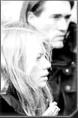
\includegraphics{graphics/nikita}&
%\begin{minipage}{0.63\textwidth}
%\vspace{-12em}

I recently watched a TV show
called La Femme Nikita about a woman
named Nikita who is forced to be an agent for a shady
anti-terrorist organization
called Section One.  Nikita has strong feelings for fellow agent
Michael, and she most trusts Walter, Section One's
ex-biker gadgets and explosives expert.  Often Nikita's worst enemies
are her superiors and coworkers at Section One.
%\end{minipage}
%\end{tabular}
%\hspace{1em}
A synopsis for a Season Three episode is as follows:

\begin{quote}
PLAYING WITH FIRE

On a mission to secure detonation chips from a terrorist
organization's heavily armed base camp, Nikita is captured as a
hostage by the enemy.  Or so it is made to look.  Michael and Nikita
have actually created the scenario in order to secretly rendezvous
with each other. The ruse works, but when Birkoff [Section One's
master hacker] accidentally discovers encrypted messages between
Michael and Nikita sent with Walter's help, Birkoff is forced to tell
Madeline.  Suspecting that Michael and Nikita may be planning a coup
d'\'etat, Operations and Madeline use a second team of operatives to
track Michael and Nikita's next secret rendezvous... killing them if
necessary.
\end{quote}


What sort of encryption might Walter have helped them to use? I let my
imagination run free, and this is what I came up with.  After being
captured at the base camp, Nikita is given a phone by her captors in
hopes that she'll use it and they'll be able to figure out what she is
really up to.  Everyone is eagerly listening in on her calls.

\begin{remark}
  In this book, we will assume a method is available for producing
  random integers.  Methods for generating random integers are
  involved and interesting, but we will not discuss them in this book.
  For an in-depth treatment of random numbers, see
  \cite[Ch.~3]{knuth2}.
\end{remark}

Nikita remembers a conversation with Walter about a public-key
cryptosystem called the ``Diffie-Hellman key exchange.''  She
remembers that it allows two people to agree on a secret key in the
presence of eavesdroppers.  Moreover, Walter mentioned that though
Diffie-Hellman\index{Diffie-Hellman cryptosystem}\index{cryptosystem!Diffie-Hellman}
was the first ever public-key exchange system, it is still in
common use today (for example, in OpenSSH protocol version 2,
see \url{http://www.openssh.com/}).

\begin{figure}
\begin{center}
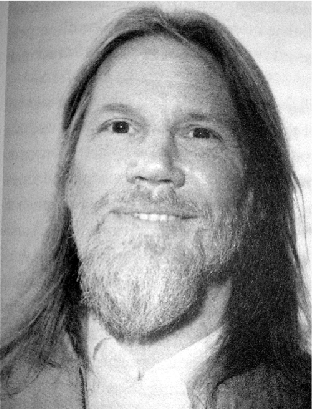
\includegraphics[width=10em]{graphics/diffie}
$\qquad$
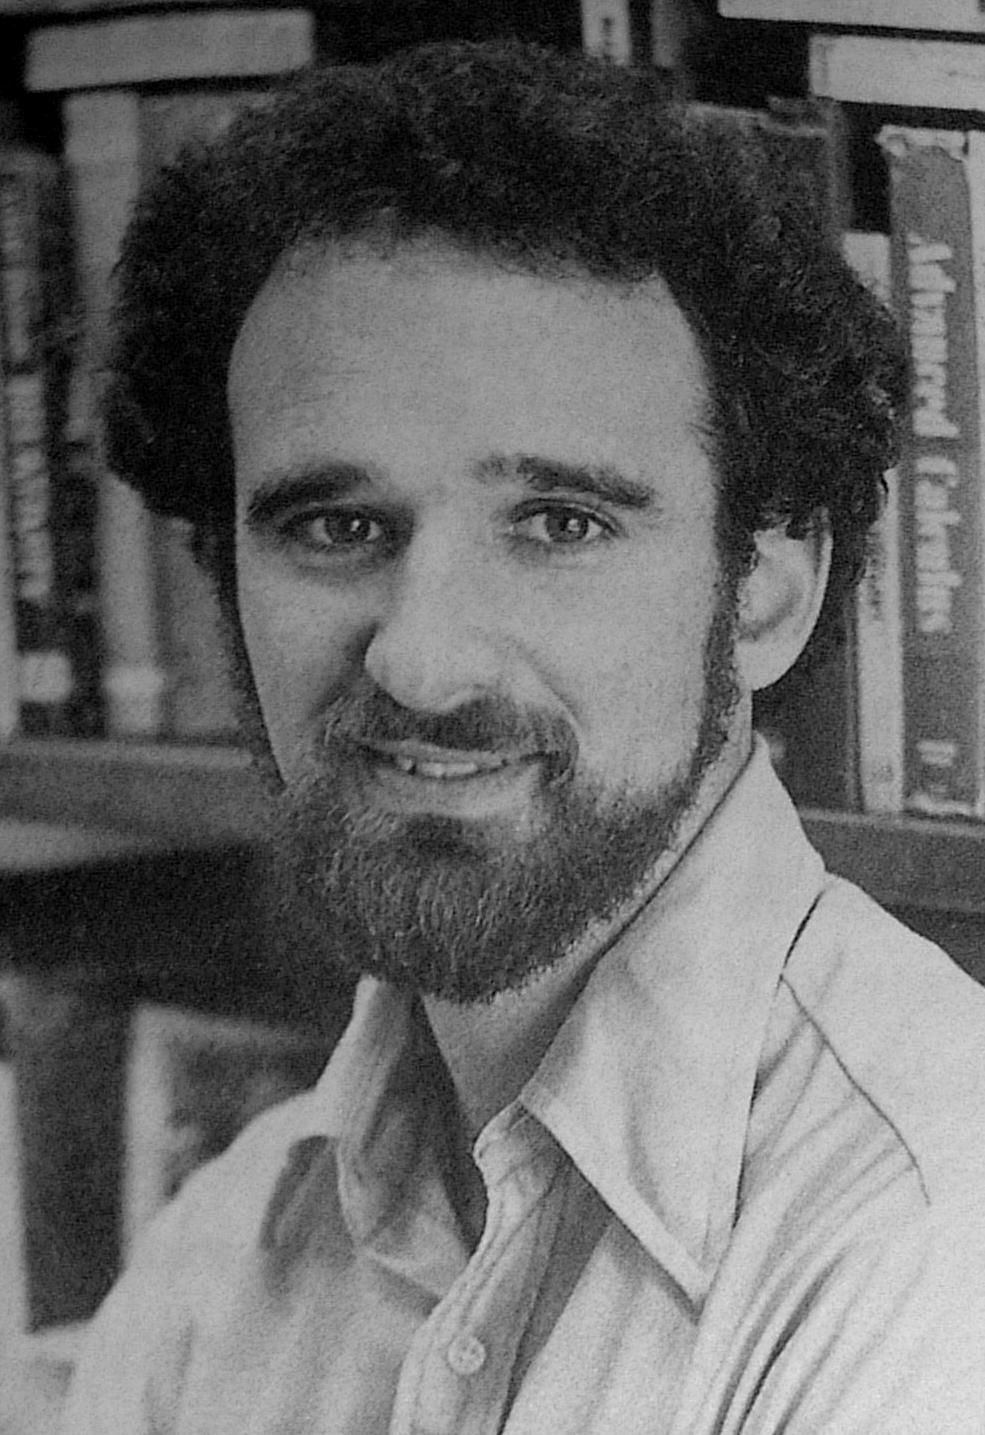
\includegraphics[width=10em]{graphics/hellman}
\end{center}
\caption{Diffie and Hellman (photos from
\cite{singh:crypto})}
\end{figure}



Nikita pulls out her handheld computer and phone,
calls up Michael, and they do the following, which
is {\em wrong} (try to figure out what is wrong as
you read it).
\begin{enumerate}
\item Together they choose a big prime number~$p$ and a number~$g$ with
$1<g<p$.
\item Nikita {\em secretly} chooses an integer~$n$.
\item Michael {\em secretly} chooses an integer~$m$.
\item Nikita tells Michael $ng \pmod{p}$.
\item Michael tells $mg\pmod{p}$ to Nikita.
\item The ``secret key'' is
$s=nmg\pmod{p}$,
which both Nikita and Michael can easily compute.
\end{enumerate}

%\begin{center}
%\includegraphics[width=0.7\textwidth]{graphics/nm_comm}
%\end{center}

Here's a very simple example with small numbers that illustrates what
Michael and Nikita do.  (They really used much larger numbers.)
\begin{center}
\shadowbox{
\begin{minipage}{.5\textwidth}
\begin{enumerate}
\item $p=97$, $g=5$
\item $n=31$
\item $m=95$
\item $ng\con 58\pmod{97}$
\item $mg \con 87\pmod{97}$
\item $s = nmg = 78\pmod{97}$
\end{enumerate}
\end{minipage}}
\end{center}

Nikita and Michael are foiled because everyone easily figures
out~$s$:
\begin{enumerate}
\item Everyone knows $p$, $g$, $ng\pmod{p}$, and $mg\pmod{p}$.
\item Using Algorithm~\ref{alg:xgcd}, anyone can
easily find $a,b\in\Z$
such that $ag + bp = 1$, which exists because
$\gcd(g,p)=1$.
\item Then, $ang \con n\pmod{p}$, so everyone knows Nikita's
secret key~$n$, and hence can easily compute the shared
secret~$s$.
\end{enumerate}

To taunt her, Nikita's captors give her a paragraph from a review of Diffie
and Hellman's 1976 paper ``New Directions in Cryptography'' \cite{dh76}:
\begin{quote}
``The authors discuss some recent results in communications theory
[...]  The first [method] has the feature that an unauthorized
`eavesdropper' will find it computationally infeasible to decipher
the message [...] They propose a couple of techniques for implementing
the system, but the reviewer was unconvinced.''
\end{quote}

\section{The Diffie-Hellman Key Exchange}\label{sec:diffie}
\index{Diffie-Hellman cryptosystem|nn}\index{cryptosystem!Diffie-Hellman|nn}
As night darkens Nikita's cell, she reflects on what has happened.
Upon realizing that she mis-remembered how the system works, she phones
Michael and they do the following:
\begin{enumerate}
\item Together Michael and Nikita choose a 200-digit integer~$p$ that
  is likely to be prime (see Section~\ref{sec:prob_prime_test}), and
  choose a number~$g$ with $1<g<p$.
\item Nikita {\em secretly} chooses an integer~$n$.
\item Michael {\em secretly} chooses an integer~$m$.
\item Nikita computes $g^n\pmod{p}$ on her handheld computer and tells
Michael the resulting number over the phone.
\item Michael tells Nikita $g^m\pmod{p}$.
\item The shared secret key is then
   $$
      s\con (g^n)^m \con (g^m)^n \con g^{nm}\pmod{p},
   $$
which both Nikita and Michael can compute.
\end{enumerate}

Here is a simplified example that illustrates what they did, that
involves only relatively simple arithmetic.
\begin{center}
\shadowbox{
\begin{minipage}{.5\textwidth}
\begin{enumerate}
\item $p = 97$, $g=5$
\item $n = 31$
\item $m = 95$
\item $g^n \con 7 \pmod{p}$
\item $g^m\con 39\pmod{p}$
\item $s \con (g^n)^m \con 14\pmod{p}$
\end{enumerate}
\end{minipage}}
\end{center}


\subsection{The Discrete Log Problem}\label{sec:dlog}
\index{discrete log problem} Nikita communicates with Michael by
encrypting everything using their agreed upon secret key (for example, using
a standard symmetric cipher such as AES, Arcfour, Cast128, 3DES, or
Blowfish).  In order to understand the conversation, the eavesdropper
needs~$s$, but it takes a long time to compute~$s$ given
only~$p$,~$g$, $g^n$, and $g^m$.  One way would be to compute~$n$ from
knowledge of~$g$ and $g^n$; this is possible, but appears to be
``computationally infeasible,'' in the sense that it would take too
long to be practical.

Let~$a$,~$b$, and~$n$ be real numbers with
$a,b>0$ and $n\geq 0$.
Recall that the ``log to the base $b$'' function is
characterized by
$$
  \log_b(a) = n \text{ if and only if } a=b^n.
$$
We use the $\log_b$ function
in algebra to solve
the following problem:
Given a base~$b$ and a power~$a$ of~$b$,
find an exponent~$n$ such that
$$
   a = b^n.
$$
That is, given $a=b^n$ and~$b$, find~$n$.

\begin{sg}
The number $a = 19683$ is the
$n$th power of $b=3$ for some~$n$. We quickly find
that
$$
  n = \log_3(19683) = \log(19683) / \log(3) = 9.
$$
\begin{verbatim}
sage: log(19683.0)
9.88751059801299
sage: log(3.0)
1.09861228866811
sage: log(19683.0) / log(3.0)
9.00000000000000
\end{verbatim}
\sage can quickly compute a numerical approximation for $\log(x)$, for
any $x$, by computing a partial sum of an appropriate
rapidly-converging infinite series (at least for $x$ in a certain
range).
\end{sg}

The discrete log problem is the analog of computing $\log_b(a)$  but
where both $b$ and $a$ are elements of a finite group.
\begin{problem}[Discrete Log Problem]\label{prob:log}\index{discrete log problem}
Let~$G$ be a finite group, for example, $G=(\zmod{p})^*$.  Given $b\in G$ and
a power~$a$ of~$b$, find a positive integer~$n$ such that
$b^n=a$.
\end{problem}

As far as we know, finding discrete logarithms in $(\zmod{p})^*$
when $p$ is large is
``very difficult'' in practice.  Over the years, many people have been
very motivated to try.  For example, if Nikita's captors could
efficiently solve Problem~\ref{prob:log}, then they could read the
messages she exchanges with Michael.  Unfortunately, we have no formal
proof that computing discrete logarithms on a classical computer is
difficult.  \index{discrete log problem!difficulty of} Also, Peter
Shor \cite{shor}\index{Shor} showed that if one could build a
sufficiently complicated quantum computer,\index{quantum computer} it
could solve the discrete logarithm problem in time bounded by a
polynomial function of the number of digits of $\#G$.

It is easy to give an inefficient algorithm that solves the discrete
log problem.  Simply try $b^1$, $b^2$, $b^3$, etc., until we find an
exponent~$n$ such that $b^n=a$.  For example, suppose $a = 18$, $b=5$,
and $p=23$.  Working modulo $23$, we have
$$b^1 = 5,\, b^2 = 2,\, b^3 = 10,\, \ldots,\, b^{12} = 18,$$
so $n=12$.
When~$p$ is large, computing the discrete log this way soon becomes
impractical, because increasing the number of digits of the modulus
makes the computation take vastly longer.


\begin{sg}
Perhaps part of the reason that computing discrete logarithms is
difficult, is that the logarithm in the real numbers is continuous,
but the (minimum) logarithm of a number mod $n$ bounces around at
random.  We illustrate this exotic behavior in Figure~\ref{fig:logs}.

This draws the continuous plot.
\begin{verbatim}
sage: plot(log, 0.1,10, rgbcolor=(0,0,1))
\end{verbatim}

This draws the discrete plot.
\begin{verbatim}
sage: p = 53
sage: R = Integers(p)
sage: a = R.multiplicative_generator()
sage: v = sorted([(a^n, n) for n in range(p-1)])
sage: G = plot(point(v,pointsize=50,rgbcolor=(0,0,1)))
sage: H = plot(line(v,rgbcolor=(0.5,0.5,0.5)))
sage: G + H
\end{verbatim}

\begin{figure}
\begin{center}
%%%%%%%%%%%%%%%%%%%%%%%%%%%%%%%%%%%%%%%%%%%%%%%%%%%%%%%%%%%%%%%%%%%%%%
% Graph: log
%% (Contact: William Stein, http://modular.fas.harvard.edu)
%%%%%%%%%%%%%%%%%%%%%%%%%%%%%%%%%%%%%%%%%%%%%%%%%%%%%%%%%%%%%%%%%%%%%
\psset{unit=0.9}
\pspicture(-1.000,-3.000)(11.000,2.500)
\newrgbcolor{mycolor}{0.00 0.00 0.00}\mycolor
%RGB color (0.0, 0.0, 0.0)
\newrgbcolor{mycolor}{0.00 0.00 0.00}\mycolor

%$x$-$y$ axes
\psline[linecolor=mycolor]{->}(-1.000,0.000)(11.000,0.000)
\rput[lb](11.300,0.000){$x$}
\psline[linecolor=mycolor]{->}(0.000,-3.000)(0.000,2.500)
\rput[lb](0.000,2.800){$y$}

%Axes tick marks
\psline[linecolor=mycolor]{-}(1.0, -0.10000000000000001)(1.0, 0.10000000000000001)
\rput[b](1.0, 0.20000000000000001){1}
\psline[linecolor=mycolor]{-}(2.0, -0.10000000000000001)(2.0, 0.10000000000000001)
\rput[b](2.0, 0.20000000000000001){2}
\psline[linecolor=mycolor]{-}(3.0, -0.10000000000000001)(3.0, 0.10000000000000001)
\rput[b](3.0, 0.20000000000000001){3}
\psline[linecolor=mycolor]{-}(4.0, -0.10000000000000001)(4.0, 0.10000000000000001)
\rput[b](4.0, 0.20000000000000001){4}
\psline[linecolor=mycolor]{-}(5.0, -0.10000000000000001)(5.0, 0.10000000000000001)
\rput[b](5.0, 0.20000000000000001){5}
\psline[linecolor=mycolor]{-}(6.0, -0.10000000000000001)(6.0, 0.10000000000000001)
\rput[b](6.0, 0.20000000000000001){6}
\psline[linecolor=mycolor]{-}(7.0, -0.10000000000000001)(7.0, 0.10000000000000001)
\rput[b](7.0, 0.20000000000000001){7}
\psline[linecolor=mycolor]{-}(8.0, -0.10000000000000001)(8.0, 0.10000000000000001)
\rput[b](8.0, 0.20000000000000001){8}
\psline[linecolor=mycolor]{-}(9.0, -0.10000000000000001)(9.0, 0.10000000000000001)
\rput[b](9.0, 0.20000000000000001){9}
\psline[linecolor=mycolor]{-}(10.0, -0.10000000000000001)(10.0, 0.10000000000000001)
\rput[b](10.0, 0.20000000000000001){10}
\psline[linecolor=mycolor]{-}(-0.04583333333333333, -3.0)(0.04583333333333333, -3.0)
\rput[b](0.27499999999999997, -3.0916666666666668){-3}
\psline[linecolor=mycolor]{-}(-0.04583333333333333, -2.0)(0.04583333333333333, -2.0)
\rput[b](0.27499999999999997, -2.0916666666666668){-2}
\psline[linecolor=mycolor]{-}(-0.04583333333333333, -1.0)(0.04583333333333333, -1.0)
\rput[b](0.27499999999999997, -1.0916666666666666){-1}
\psline[linecolor=mycolor]{-}(-0.04583333333333333, 1.0)(0.04583333333333333, 1.0)
\rput[b](0.27499999999999997, 0.90833333333333333){1}

%RGB color (0.20000000000000001, 0.20000000000000001, 1.0)
\newrgbcolor{mycolor}{0.20 0.20 1.00}\mycolor

%Curve defined by 99 points
\pscurve[linecolor=mycolor](0.10000000000000001, -2.3025850929940455)(0.20000000000000001, -1.6094379124341003)(0.30000000000000004, -1.2039728043259359)(0.40000000000000002, -0.916290731874155)(0.5, -0.69314718055994529)(0.60000000000000009, -0.5108256237659905)(0.70000000000000007, -0.35667494393873228)(0.80000000000000004, -0.22314355131420971)(0.90000000000000002, -0.10536051565782628)(1.0, 0.0)(1.1000000000000001, 0.095310179804324935)(1.2000000000000002, 0.18232155679395479)(1.3, 0.26236426446749106)(1.4000000000000001, 0.33647223662121301)(1.5, 0.40546510810816438)(1.6000000000000001, 0.47000362924573563)(1.7000000000000002, 0.53062825106217049)(1.8, 0.58778666490211906)(1.9000000000000001, 0.64185388617239481)(2.0, 0.69314718055994529)(2.1000000000000001, 0.74193734472937733)(2.2000000000000002, 0.78845736036427028)(2.3000000000000003, 0.83290912293510411)(2.4000000000000004, 0.87546873735390007)(2.5, 0.91629073187415511)(2.6000000000000001, 0.95551144502743635)(2.7000000000000002, 0.99325177301028345)(2.8000000000000003, 1.0296194171811583)(2.9000000000000004, 1.0647107369924285)(3.0, 1.0986122886681098)(3.1000000000000001, 1.1314021114911006)(3.2000000000000002, 1.1631508098056809)(3.3000000000000003, 1.1939224684724346)(3.4000000000000004, 1.2237754316221159)(3.5, 1.2527629684953681)(3.6000000000000001, 1.2809338454620642)(3.7000000000000002, 1.3083328196501789)(3.8000000000000003, 1.3350010667323402)(3.9000000000000004, 1.3609765531356008)(4.0, 1.3862943611198906)(4.1000000000000005, 1.4109869737102623)(4.2000000000000002, 1.4350845252893227)(4.2999999999999998, 1.4586150226995167)(4.4000000000000004, 1.4816045409242156)(4.5, 1.5040773967762742)(4.6000000000000005, 1.5260563034950494)(4.7000000000000002, 1.547562508716013)(4.8000000000000007, 1.5686159179138455)(4.9000000000000004, 1.589235205116581)(5.0, 1.6094379124341003)(5.1000000000000005, 1.6292405397302803)(5.2000000000000002, 1.6486586255873816)(5.3000000000000007, 1.6677068205580763)(5.4000000000000004, 1.6863989535702288)(5.5, 1.7047480922384253)(5.6000000000000005, 1.7227665977411037)(5.7000000000000002, 1.7404661748405046)(5.8000000000000007, 1.7578579175523739)(5.9000000000000004, 1.7749523509116738)(6.0, 1.791759469228055)(6.1000000000000005, 1.8082887711792657)(6.2000000000000002, 1.824549292051046)(6.3000000000000007, 1.8405496333974871)(6.4000000000000004, 1.8562979903656263)(6.5, 1.8718021769015913)(6.6000000000000005, 1.8870696490323799)(6.7000000000000002, 1.9021075263969205)(6.8000000000000007, 1.9169226121820611)(6.9000000000000004, 1.9315214116032138)(7.0, 1.9459101490553132)(7.1000000000000005, 1.9600947840472698)(7.2000000000000002, 1.9740810260220096)(7.3000000000000007, 1.9878743481543455)(7.4000000000000004, 2.0014800002101243)(7.5, 2.0149030205422647)(7.6000000000000005, 2.0281482472922856)(7.7000000000000002, 2.0412203288596382)(7.8000000000000007, 2.0541237336955462)(7.9000000000000004, 2.066862759472976)(8.0, 2.0794415416798357)(8.0999999999999996, 2.0918640616783932)(8.2000000000000011, 2.1041341542702074)(8.3000000000000007, 2.1162555148025524)(8.4000000000000004, 2.1282317058492679)(8.5, 2.1400661634962708)(8.5999999999999996, 2.1517622032594619)(8.7000000000000011, 2.1633230256605382)(8.8000000000000007, 2.174751721484161)(8.9000000000000004, 2.1860512767380942)(9.0, 2.1972245773362196)(9.0999999999999996, 2.2082744135228043)(9.2000000000000011, 2.2192034840549946)(9.3000000000000007, 2.2300144001592104)(9.4000000000000004, 2.2407096892759584)(9.5, 2.2512917986064953)(9.6000000000000014, 2.2617630984737906)(9.7000000000000011, 2.2721258855093374)(9.8000000000000007, 2.2823823856765264)(9.9000000000000004, 2.2925347571405443)
%RGB color (0.0, 0.0, 0.0)
\newrgbcolor{mycolor}{0.00 0.00 0.00}\mycolor

\endpspicture
%%%%%%%%%%%%%%%%%%%%%%%%%%%%%%%%%%%%%%%%%%%%%%%%%%%%%%%%%%%%%%%%%%%%%

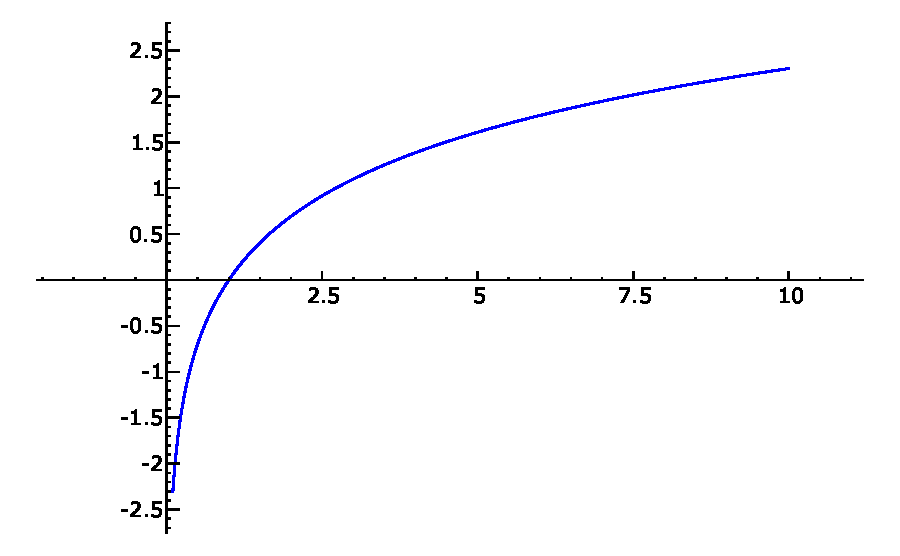
\includegraphics[width=0.47\textwidth]{graphics/log}
%\vspace{5ex}
%%%%%%%%%%%%%%%%%%%%%%%%%%%%%%%%%%%%%%%%%%%%%%%%%%%%%%%%%%%%%%%%%%%%%%
% Graph: dlog
%% (Contact: William Stein, http://modular.fas.harvard.edu)
%%%%%%%%%%%%%%%%%%%%%%%%%%%%%%%%%%%%%%%%%%%%%%%%%%%%%%%%%%%%%%%%%%%%%
\psset{unit=0.1}
\pspicture(-1.000,-1.000)(100.000,100.000)
\newrgbcolor{mycolor}{0.00 0.00 0.00}\mycolor
%$x$-$y$ axes
\psline[linecolor=mycolor]{->}(-1.000,0.000)(100.000,0.000)
\rput[lb](100.300,0.000){$x$}
\psline[linecolor=mycolor]{->}(0.000,-1.000)(0.000,100.000)
\rput[lb](0.000,100.300){$y$}

%Axes tick marks
\psline[linecolor=mycolor]{-}(10.0, -0.84166666666666667)(10.0, 0.84166666666666667)
\rput[b](10.0, -5.0499999999999998){10}
\psline[linecolor=mycolor]{-}(20.0, -0.84166666666666667)(20.0, 0.84166666666666667)
\rput[b](20.0, -5.0499999999999998){20}
\psline[linecolor=mycolor]{-}(30.0, -0.84166666666666667)(30.0, 0.84166666666666667)
\rput[b](30.0, -5.0499999999999998){30}
\psline[linecolor=mycolor]{-}(40.0, -0.84166666666666667)(40.0, 0.84166666666666667)
\rput[b](40.0, -5.0499999999999998){40}
\psline[linecolor=mycolor]{-}(50.0, -0.84166666666666667)(50.0, 0.84166666666666667)
\rput[b](50.0, -5.0499999999999998){50}
\psline[linecolor=mycolor]{-}(60.0, -0.84166666666666667)(60.0, 0.84166666666666667)
\rput[b](60.0, -5.0499999999999998){60}
\psline[linecolor=mycolor]{-}(70.0, -0.84166666666666667)(70.0, 0.84166666666666667)
\rput[b](70.0, -5.0499999999999998){70}
\psline[linecolor=mycolor]{-}(80.0, -0.84166666666666667)(80.0, 0.84166666666666667)
\rput[b](80.0, -5.0499999999999998){80}
\psline[linecolor=mycolor]{-}(90.0, -0.84166666666666667)(90.0, 0.84166666666666667)
\rput[b](90.0, -5.0499999999999998){90}
\psline[linecolor=mycolor]{-}(-0.84166666666666667, 10.0)(0.84166666666666667, 10.0)
\rput[b](-5.0499999999999998, 8.3166666666666664){10}
\psline[linecolor=mycolor]{-}(-0.84166666666666667, 20.0)(0.84166666666666667, 20.0)
\rput[b](-5.0499999999999998, 18.316666666666666){20}
\psline[linecolor=mycolor]{-}(-0.84166666666666667, 30.0)(0.84166666666666667, 30.0)
\rput[b](-5.0499999999999998, 28.316666666666666){30}
\psline[linecolor=mycolor]{-}(-0.84166666666666667, 40.0)(0.84166666666666667, 40.0)
\rput[b](-5.0499999999999998, 38.31666666666667){40}
\psline[linecolor=mycolor]{-}(-0.84166666666666667, 50.0)(0.84166666666666667, 50.0)
\rput[b](-5.0499999999999998, 48.31666666666667){50}
\psline[linecolor=mycolor]{-}(-0.84166666666666667, 60.0)(0.84166666666666667, 60.0)
\rput[b](-5.0499999999999998, 58.31666666666667){60}
\psline[linecolor=mycolor]{-}(-0.84166666666666667, 70.0)(0.84166666666666667, 70.0)
\rput[b](-5.0499999999999998, 68.316666666666663){70}
\psline[linecolor=mycolor]{-}(-0.84166666666666667, 80.0)(0.84166666666666667, 80.0)
\rput[b](-5.0499999999999998, 78.316666666666663){80}
\psline[linecolor=mycolor]{-}(-0.84166666666666667, 90.0)(0.84166666666666667, 90.0)
\rput[b](-5.0499999999999998, 88.316666666666663){90}

%RGB color (0.20000000000000001, 0.20000000000000001, 1.0)
\newrgbcolor{mycolor}{0.20 0.20 1.00}\mycolor

%Solid dot at (5.000,1.000) of radius 0.3
\pscircle*[linecolor=mycolor](5.000,1.000){0.300}
%Solid dot at (25.000,2.000) of radius 0.3
\pscircle*[linecolor=mycolor](25.000,2.000){0.300}
%Solid dot at (28.000,3.000) of radius 0.3
\pscircle*[linecolor=mycolor](28.000,3.000){0.300}
%Solid dot at (43.000,4.000) of radius 0.3
\pscircle*[linecolor=mycolor](43.000,4.000){0.300}
%Solid dot at (21.000,5.000) of radius 0.3
\pscircle*[linecolor=mycolor](21.000,5.000){0.300}
%Solid dot at (8.000,6.000) of radius 0.3
\pscircle*[linecolor=mycolor](8.000,6.000){0.300}
%Solid dot at (40.000,7.000) of radius 0.3
\pscircle*[linecolor=mycolor](40.000,7.000){0.300}
%Solid dot at (6.000,8.000) of radius 0.3
\pscircle*[linecolor=mycolor](6.000,8.000){0.300}
%Solid dot at (30.000,9.000) of radius 0.3
\pscircle*[linecolor=mycolor](30.000,9.000){0.300}
%Solid dot at (53.000,10.000) of radius 0.3
\pscircle*[linecolor=mycolor](53.000,10.000){0.300}
%Solid dot at (71.000,11.000) of radius 0.3
\pscircle*[linecolor=mycolor](71.000,11.000){0.300}
%Solid dot at (64.000,12.000) of radius 0.3
\pscircle*[linecolor=mycolor](64.000,12.000){0.300}
%Solid dot at (29.000,13.000) of radius 0.3
\pscircle*[linecolor=mycolor](29.000,13.000){0.300}
%Solid dot at (48.000,14.000) of radius 0.3
\pscircle*[linecolor=mycolor](48.000,14.000){0.300}
%Solid dot at (46.000,15.000) of radius 0.3
\pscircle*[linecolor=mycolor](46.000,15.000){0.300}
%Solid dot at (36.000,16.000) of radius 0.3
\pscircle*[linecolor=mycolor](36.000,16.000){0.300}
%Solid dot at (83.000,17.000) of radius 0.3
\pscircle*[linecolor=mycolor](83.000,17.000){0.300}
%Solid dot at (27.000,18.000) of radius 0.3
\pscircle*[linecolor=mycolor](27.000,18.000){0.300}
%Solid dot at (38.000,19.000) of radius 0.3
\pscircle*[linecolor=mycolor](38.000,19.000){0.300}
%Solid dot at (93.000,20.000) of radius 0.3
\pscircle*[linecolor=mycolor](93.000,20.000){0.300}
%Solid dot at (77.000,21.000) of radius 0.3
\pscircle*[linecolor=mycolor](77.000,21.000){0.300}
%Solid dot at (94.000,22.000) of radius 0.3
\pscircle*[linecolor=mycolor](94.000,22.000){0.300}
%Solid dot at (82.000,23.000) of radius 0.3
\pscircle*[linecolor=mycolor](82.000,23.000){0.300}
%Solid dot at (22.000,24.000) of radius 0.3
\pscircle*[linecolor=mycolor](22.000,24.000){0.300}
%Solid dot at (13.000,25.000) of radius 0.3
\pscircle*[linecolor=mycolor](13.000,25.000){0.300}
%Solid dot at (65.000,26.000) of radius 0.3
\pscircle*[linecolor=mycolor](65.000,26.000){0.300}
%Solid dot at (34.000,27.000) of radius 0.3
\pscircle*[linecolor=mycolor](34.000,27.000){0.300}
%Solid dot at (73.000,28.000) of radius 0.3
\pscircle*[linecolor=mycolor](73.000,28.000){0.300}
%Solid dot at (74.000,29.000) of radius 0.3
\pscircle*[linecolor=mycolor](74.000,29.000){0.300}
%Solid dot at (79.000,30.000) of radius 0.3
\pscircle*[linecolor=mycolor](79.000,30.000){0.300}
%Solid dot at (7.000,31.000) of radius 0.3
\pscircle*[linecolor=mycolor](7.000,31.000){0.300}
%Solid dot at (35.000,32.000) of radius 0.3
\pscircle*[linecolor=mycolor](35.000,32.000){0.300}
%Solid dot at (78.000,33.000) of radius 0.3
\pscircle*[linecolor=mycolor](78.000,33.000){0.300}
%Solid dot at (2.000,34.000) of radius 0.3
\pscircle*[linecolor=mycolor](2.000,34.000){0.300}
%Solid dot at (10.000,35.000) of radius 0.3
\pscircle*[linecolor=mycolor](10.000,35.000){0.300}
%Solid dot at (50.000,36.000) of radius 0.3
\pscircle*[linecolor=mycolor](50.000,36.000){0.300}
%Solid dot at (56.000,37.000) of radius 0.3
\pscircle*[linecolor=mycolor](56.000,37.000){0.300}
%Solid dot at (86.000,38.000) of radius 0.3
\pscircle*[linecolor=mycolor](86.000,38.000){0.300}
%Solid dot at (42.000,39.000) of radius 0.3
\pscircle*[linecolor=mycolor](42.000,39.000){0.300}
%Solid dot at (16.000,40.000) of radius 0.3
\pscircle*[linecolor=mycolor](16.000,40.000){0.300}
%Solid dot at (80.000,41.000) of radius 0.3
\pscircle*[linecolor=mycolor](80.000,41.000){0.300}
%Solid dot at (12.000,42.000) of radius 0.3
\pscircle*[linecolor=mycolor](12.000,42.000){0.300}
%Solid dot at (60.000,43.000) of radius 0.3
\pscircle*[linecolor=mycolor](60.000,43.000){0.300}
%Solid dot at (9.000,44.000) of radius 0.3
\pscircle*[linecolor=mycolor](9.000,44.000){0.300}
%Solid dot at (45.000,45.000) of radius 0.3
\pscircle*[linecolor=mycolor](45.000,45.000){0.300}
%Solid dot at (31.000,46.000) of radius 0.3
\pscircle*[linecolor=mycolor](31.000,46.000){0.300}
%Solid dot at (58.000,47.000) of radius 0.3
\pscircle*[linecolor=mycolor](58.000,47.000){0.300}
%Solid dot at (96.000,48.000) of radius 0.3
\pscircle*[linecolor=mycolor](96.000,48.000){0.300}
%Solid dot at (92.000,49.000) of radius 0.3
\pscircle*[linecolor=mycolor](92.000,49.000){0.300}
%Solid dot at (72.000,50.000) of radius 0.3
\pscircle*[linecolor=mycolor](72.000,50.000){0.300}
%Solid dot at (69.000,51.000) of radius 0.3
\pscircle*[linecolor=mycolor](69.000,51.000){0.300}
%Solid dot at (54.000,52.000) of radius 0.3
\pscircle*[linecolor=mycolor](54.000,52.000){0.300}
%Solid dot at (76.000,53.000) of radius 0.3
\pscircle*[linecolor=mycolor](76.000,53.000){0.300}
%Solid dot at (89.000,54.000) of radius 0.3
\pscircle*[linecolor=mycolor](89.000,54.000){0.300}
%Solid dot at (57.000,55.000) of radius 0.3
\pscircle*[linecolor=mycolor](57.000,55.000){0.300}
%Solid dot at (91.000,56.000) of radius 0.3
\pscircle*[linecolor=mycolor](91.000,56.000){0.300}
%Solid dot at (67.000,57.000) of radius 0.3
\pscircle*[linecolor=mycolor](67.000,57.000){0.300}
%Solid dot at (44.000,58.000) of radius 0.3
\pscircle*[linecolor=mycolor](44.000,58.000){0.300}
%Solid dot at (26.000,59.000) of radius 0.3
\pscircle*[linecolor=mycolor](26.000,59.000){0.300}
%Solid dot at (33.000,60.000) of radius 0.3
\pscircle*[linecolor=mycolor](33.000,60.000){0.300}
%Solid dot at (68.000,61.000) of radius 0.3
\pscircle*[linecolor=mycolor](68.000,61.000){0.300}
%Solid dot at (49.000,62.000) of radius 0.3
\pscircle*[linecolor=mycolor](49.000,62.000){0.300}
%Solid dot at (51.000,63.000) of radius 0.3
\pscircle*[linecolor=mycolor](51.000,63.000){0.300}
%Solid dot at (61.000,64.000) of radius 0.3
\pscircle*[linecolor=mycolor](61.000,64.000){0.300}
%Solid dot at (14.000,65.000) of radius 0.3
\pscircle*[linecolor=mycolor](14.000,65.000){0.300}
%Solid dot at (70.000,66.000) of radius 0.3
\pscircle*[linecolor=mycolor](70.000,66.000){0.300}
%Solid dot at (59.000,67.000) of radius 0.3
\pscircle*[linecolor=mycolor](59.000,67.000){0.300}
%Solid dot at (4.000,68.000) of radius 0.3
\pscircle*[linecolor=mycolor](4.000,68.000){0.300}
%Solid dot at (20.000,69.000) of radius 0.3
\pscircle*[linecolor=mycolor](20.000,69.000){0.300}
%Solid dot at (3.000,70.000) of radius 0.3
\pscircle*[linecolor=mycolor](3.000,70.000){0.300}
%Solid dot at (15.000,71.000) of radius 0.3
\pscircle*[linecolor=mycolor](15.000,71.000){0.300}
%Solid dot at (75.000,72.000) of radius 0.3
\pscircle*[linecolor=mycolor](75.000,72.000){0.300}
%Solid dot at (84.000,73.000) of radius 0.3
\pscircle*[linecolor=mycolor](84.000,73.000){0.300}
%Solid dot at (32.000,74.000) of radius 0.3
\pscircle*[linecolor=mycolor](32.000,74.000){0.300}
%Solid dot at (63.000,75.000) of radius 0.3
\pscircle*[linecolor=mycolor](63.000,75.000){0.300}
%Solid dot at (24.000,76.000) of radius 0.3
\pscircle*[linecolor=mycolor](24.000,76.000){0.300}
%Solid dot at (23.000,77.000) of radius 0.3
\pscircle*[linecolor=mycolor](23.000,77.000){0.300}
%Solid dot at (18.000,78.000) of radius 0.3
\pscircle*[linecolor=mycolor](18.000,78.000){0.300}
%Solid dot at (90.000,79.000) of radius 0.3
\pscircle*[linecolor=mycolor](90.000,79.000){0.300}
%Solid dot at (62.000,80.000) of radius 0.3
\pscircle*[linecolor=mycolor](62.000,80.000){0.300}
%Solid dot at (19.000,81.000) of radius 0.3
\pscircle*[linecolor=mycolor](19.000,81.000){0.300}
%Solid dot at (95.000,82.000) of radius 0.3
\pscircle*[linecolor=mycolor](95.000,82.000){0.300}
%Solid dot at (87.000,83.000) of radius 0.3
\pscircle*[linecolor=mycolor](87.000,83.000){0.300}
%Solid dot at (47.000,84.000) of radius 0.3
\pscircle*[linecolor=mycolor](47.000,84.000){0.300}
%Solid dot at (41.000,85.000) of radius 0.3
\pscircle*[linecolor=mycolor](41.000,85.000){0.300}
%Solid dot at (11.000,86.000) of radius 0.3
\pscircle*[linecolor=mycolor](11.000,86.000){0.300}
%Solid dot at (55.000,87.000) of radius 0.3
\pscircle*[linecolor=mycolor](55.000,87.000){0.300}
%Solid dot at (81.000,88.000) of radius 0.3
\pscircle*[linecolor=mycolor](81.000,88.000){0.300}
%Solid dot at (17.000,89.000) of radius 0.3
\pscircle*[linecolor=mycolor](17.000,89.000){0.300}
%Solid dot at (85.000,90.000) of radius 0.3
\pscircle*[linecolor=mycolor](85.000,90.000){0.300}
%Solid dot at (37.000,91.000) of radius 0.3
\pscircle*[linecolor=mycolor](37.000,91.000){0.300}
%Solid dot at (88.000,92.000) of radius 0.3
\pscircle*[linecolor=mycolor](88.000,92.000){0.300}
%Solid dot at (52.000,93.000) of radius 0.3
\pscircle*[linecolor=mycolor](52.000,93.000){0.300}
%Solid dot at (66.000,94.000) of radius 0.3
\pscircle*[linecolor=mycolor](66.000,94.000){0.300}
%Solid dot at (39.000,95.000) of radius 0.3
\pscircle*[linecolor=mycolor](39.000,95.000){0.300}
%Solid dot at (1.000,96.000) of radius 0.3
\pscircle*[linecolor=mycolor](1.000,96.000){0.300}
%RGB color (0.0, 0.0, 0.0)
\newrgbcolor{mycolor}{0.00 0.00 0.00}\mycolor

\endpspicture
%%%%%%%%%%%%%%%%%%%%%%%%%%%%%%%%%%%%%%%%%%%%%%%%%%%%%%%%%%%%%%%%%%%%%


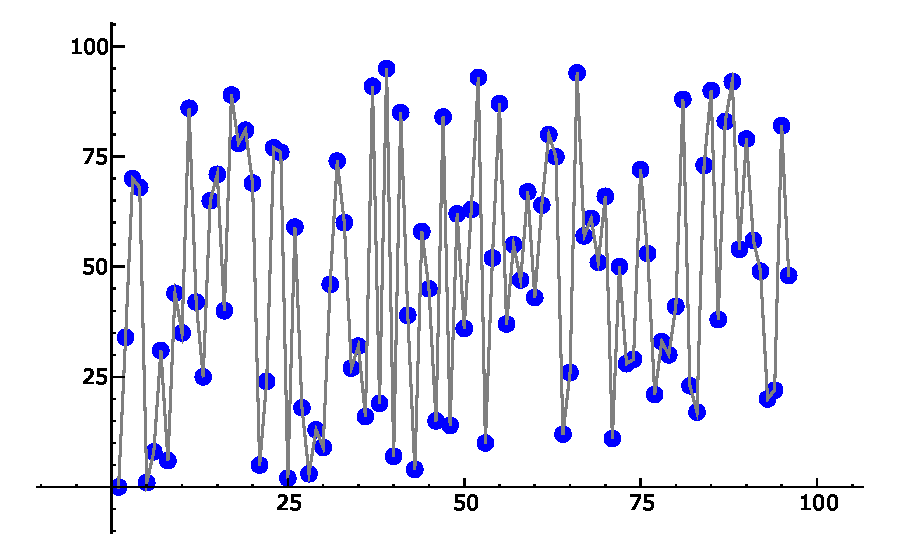
\includegraphics[width=0.47\textwidth]{graphics/dlog}
\vspace{1em}
\caption{Graphs of the continuous log and of the discrete log modulo $53$.\label{fig:logs}  Which picture looks easier to predict?}
\end{center}
\end{figure}
\end{sg}


\subsection{Realistic Diffie-Hellman Example}
In this section, we present an example that uses bigger numbers.
 First, we prove a proposition that we can use to
choose a prime~$p$ in such a way that it is easy to find a
$g\in(\zmod{p})^*$ with order $p-1$.  We have already seen
in Section~\ref{sec:primitive} that for every prime~$p$ there
exists an element~$g$ of order $p-1$, and we gave
Algorithm~\ref{alg:primitive_root} for finding a primitive
root for any prime.  The significance of Proposition~\ref{prop:pp2}
below is that it suggests an algorithm for finding
a primitive root that is easier to use in practice when~$p$
is large, because it does not require factoring $p-1$.
Of course, one could also just use a random~$g$
for Diffie-Hellman; it is not essential that~$g$
generates $(\zmod{p})^*$.

\begin{proposition}\label{prop:pp2}
Suppose~$p$ is a prime such that $(p-1)/2$ is also prime.
Then each element of $(\zmod{p})^*$ has order one of~$1$,~$2$,
$(p-1)/2$, or $p-1$.
\end{proposition}
\begin{proof}
Since~$p$ is prime, the group $(\zmod{p})^*$ is of order
$p-1$.  By assumption, the prime
factorization of $p-1$ is $2\cdot ((p-1)/2)$.  Let $a \in
(\zmod{p})^*$.  Then by Theorem~\ref{thm:fermatlittle}, $a^{p-1}=1$,
so the order of~$a$ is a divisor of $p-1$, which proves the
proposition.
\end{proof}

Given a prime~$p$ with $(p-1)/2$ prime, find an element of
order $p-1$ as follows.  If $2$ has order $p-1$, we are done.
If not, $2$ has order $(p-1)/2$ since $2$ does not have order
either $1$ or $2$.  Then $-2$ has order $p-1$.

Let $p=93450983094850938450983409611$.
Then~$p$ is prime,
but $(p-1)/2$ is not.  So we keep adding~$2$ to~$p$ and
testing pseudoprimality using algorithms from
Section~\ref{sec:prob_prime_test}
until we find that the next pseudoprime after~$p$
is
$$
q=93450983094850938450983409623.
$$
It turns out that~$q$ pseudoprime and $(q-1)/2$ is also pseudoprime.
We find that $2$ has order $(q-1)/2$, so $g=-2$ has
order $q-1$ modulo $q$, and is hence a generator of $(\zmod{q})^*$,
at least assuming that~$q$ is really prime.

The secret
random numbers generated by Nikita and Michael are
$$
  n = 18319922375531859171613379181
$$
and
$$
  m = 82335836243866695680141440300.
$$
Nikita sends
$$
  g^n = 45416776270485369791375944998 \in (\zmod{p})^*
$$
to Michael, and Michael sends
$$
  g^m = 15048074151770884271824225393\in (\zmod{p})^*
$$
to Nikita. They agree on the secret key
$$
 g^{nm} = 85771409470770521212346739540\in (\zmod{p})^*.
$$

\begin{sg}
We illustrate the above computations using \sage.
\begin{verbatim}
sage: q = 93450983094850938450983409623
sage: q.is_prime()
True
sage: is_prime((q-1)//2)
True
sage: g = Mod(-2, q)
sage: g.multiplicative_order()
93450983094850938450983409622
sage: n = 18319922375531859171613379181
sage: m = 82335836243866695680141440300
sage: g^n
45416776270485369791375944998
sage: g^m
15048074151770884271824225393
sage: (g^n)^m
85771409470770521212346739540
sage: (g^m)^n
85771409470770521212346739540
\end{verbatim}
\end{sg}

\subsection{The Man in the Middle Attack}\index{man in the middle attack|nn}
\label{sec:man_in_middle}
\par\noindent{}Since
their first system was broken, instead of talking on the phone,
Michael and Nikita can now only communicate via text messages.  One of
her captors, The Man\index{The Man}, is watching each of the
transmissions; moreover, he can intercept messages and send false
messages.  When Nikita sends a message to Michael announcing
$g^n\pmod{p}$, The Man intercepts this message, and sends his own
number $g^t\pmod{p}$ to Michael.  Eventually, Michael and The Man
agree on the secret key $g^{tm}\pmod{p}$, and Nikita and The Man agree
on the key $g^{tn}\pmod{p}$.  When Nikita sends a message to Michael
she unwittingly uses the secret key $g^{tn}\pmod{p}$; The Man then
intercepts it, decrypts it, changes it, and re-encrypts it using the
key $g^{tm}\pmod{p}$, and sends it on to Michael\index{Michael|)}.
This is bad because now The Man can read every message sent between
Michael and Nikita, and moreover, he can change them in transmission
in subtle ways.

% \begin{figure}
% \begin{center}
% \psfrag{1}{$g^{nt}\pmod{p}$}
% \psfrag{2}{$g^{nt}\pmod{p}$}
% \psfrag{3}{$g^{mt}\pmod{p}$}
% \psfrag{4}{$g^{mt}\pmod{p}$}
% 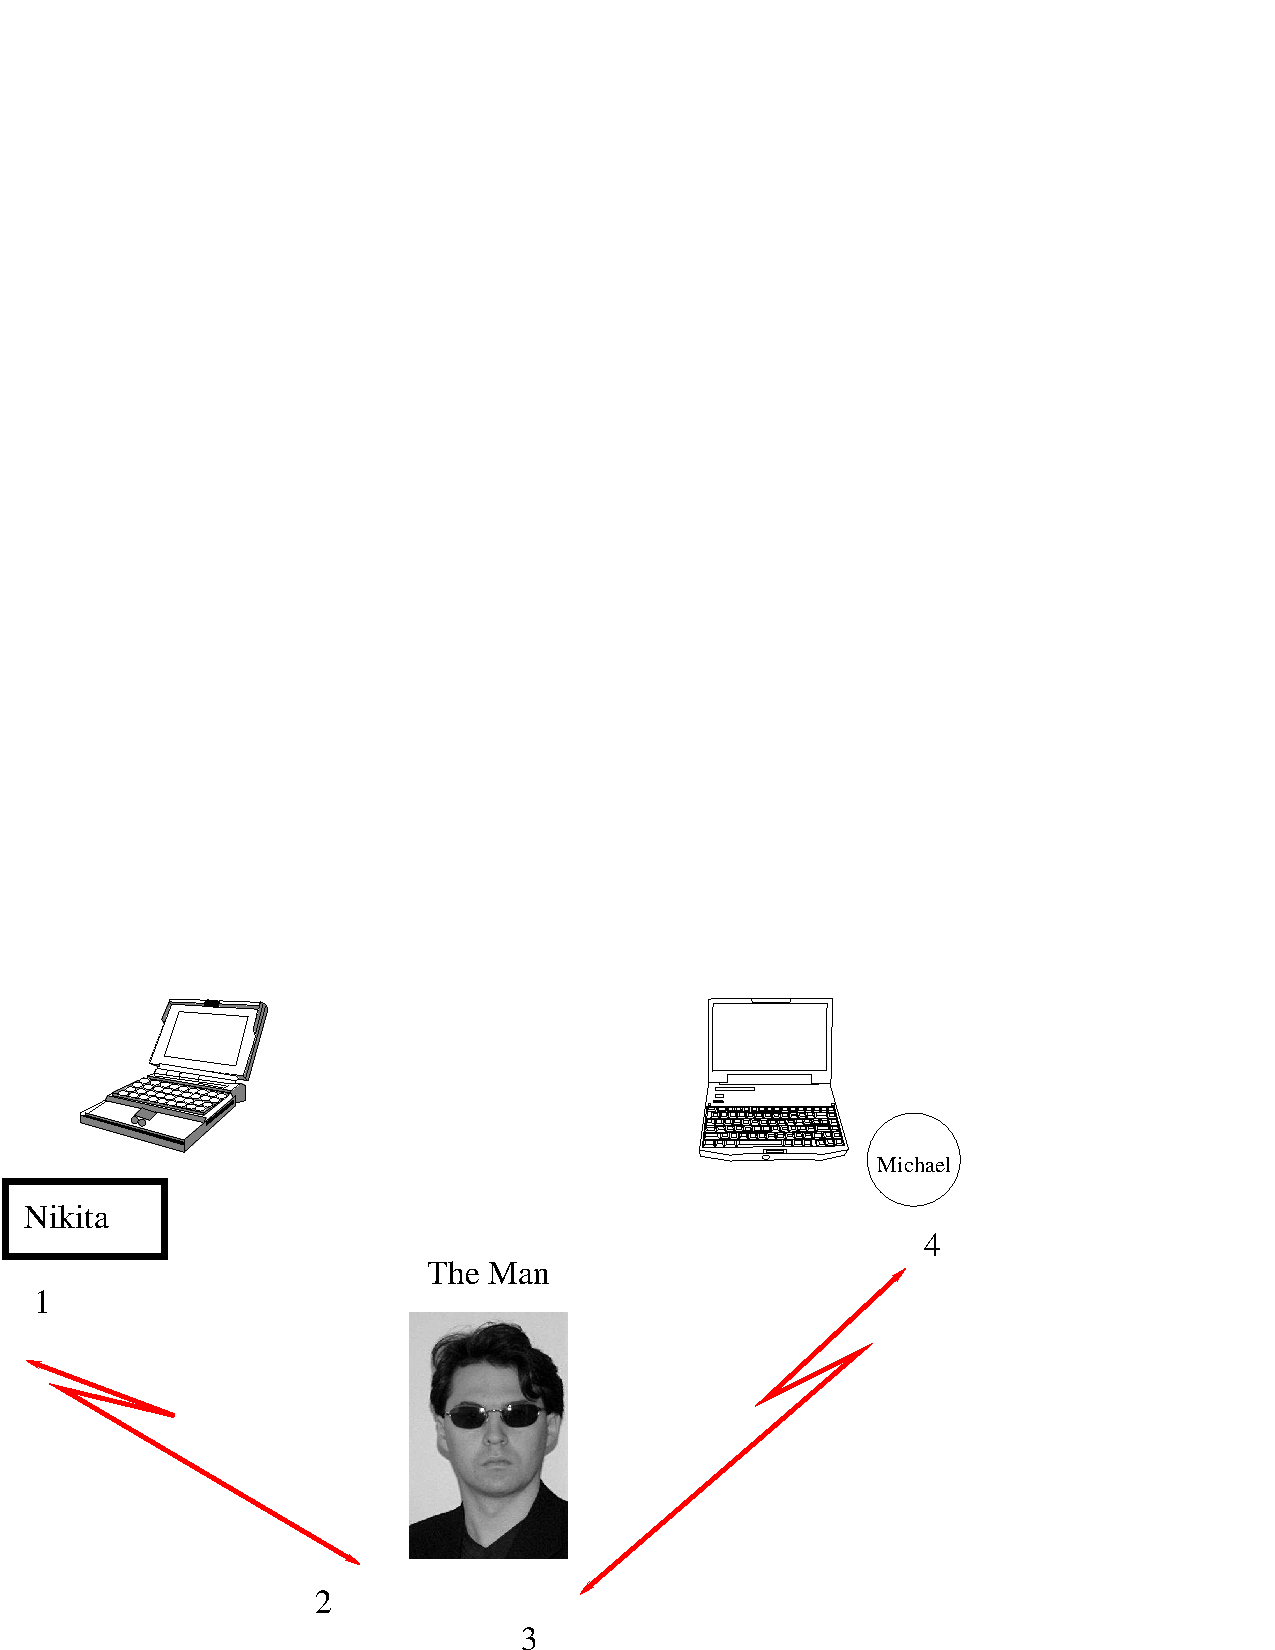
\includegraphics[width=\textwidth]{graphics/man}
% \caption{The Man in the Middle Attack}
% \end{center}

% \end{figure}

One way to get around this attack is to use a digital signature scheme
based on the RSA cryptosystem.  We will not discuss digital signatures
further \index{digital signatures} in this book, but will discuss RSA in the
next section.


\section{The RSA Cryptosystem}\index{RSA cryptosystem|(}\index{cryptosystem!RSA|(}
\label{sec:RSA}\label{sec:rsa}

The Diffie-Hellman key exchange has drawbacks.  As discussed in
Section \ref{sec:man_in_middle}, it is susceptible to the man in the
middle attack. This section is about the RSA public-key cryptosystem of
Rivest, Shamir, and Adleman \cite{rsa:origin}, which is an alternative
to Diffie-Hellman that is more flexible in some ways.

We first describe the RSA cryptosystem, then discuss several ways to
attack it.  It is important to be aware of such weaknesses, in order
to avoid foolish mistakes when implementing RSA.  We barely scratched
the surface here of the many possible attacks on specific
implementations of RSA or other cryptosystems.

\subsection{How RSA works}
The fundamental idea behind RSA is to try to construct
a trap-door or one-way function on a set~$X$.
This is an invertible function\index{one-way function|nn}
$$
     E : X \ra X
$$
such that it is easy for Nikita to compute $E^{-1}$, but extremely
difficult for anybody else to do so.



Here is how Nikita makes a one-way function~$E$
on the set of integers modulo~$n$.
\begin{enumerate}
\item Using a method hinted at in Section~\ref{sec:prob_prime_test},
Nikita picks two large primes~$p$ and~$q$, and lets $n=pq$.
\item It is then easy for Nikita to compute
$$
   \vphi(n) = \vphi(p)\cdot \vphi(q) = (p-1)\cdot (q-1).
$$
\item Nikita next chooses a random integer~$e$ with
 $$
 1<e<\vphi(n)\text{ and } \gcd(e,\vphi(n))=1.
 $$

\item Nikita uses the algorithm from Section~\ref{sec:compute_powers}
to find a solution~$x=d$ to the equation
$$
   ex \con 1\pmod{\vphi(n)}.
$$

\item Finally, Nikita defines a function $E:\zmod{n} \ra \zmod{n}$ by
$$
   E(x) = x^e \in \zmod{n}.
$$
\end{enumerate}

Note that anybody can compute~$E$ fairly quickly using the
repeated-squaring algorithm from Section~\ref{sec:compute_powers}.
Nikita's \defn{public key} is the pair of integers $(n,e)$, which is
just enough information for people to easily compute~$E$.  Nikita
knows a number~$d$ such that $ed\con 1\pmod{\vphi(n)}$, so, as we will
see, she can quickly compute $E^{-1}$.

To send Nikita a message, proceed as follows.
Encode your message, in some way, as a sequence
of numbers modulo~$n$ (see Section~\ref{sec:encode})
$$
  m_1, \ldots, m_r \in \zmod{n},
$$
then send
$$
  E(m_1), \ldots, E(m_r)
$$
to Nikita.   (Recall that $E(m) = m^e$ for $m\in \zmod{n}$.)

When Nikita receives $E(m_i)$, she finds each~$m_i$ by
using that
$
 E^{-1}(m) = m^d,
$
a fact that follows from Proposition~\ref{prop:decryptrsa}
\begin{proposition}[Decryption Key]\label{prop:decryptrsa}\iprop{decryption key}
Let~$n$ be an integer that is a product of distinct primes
and let $d,e\in\N$ be such that $p-1\mid de-1$ for each prime $p\mid n$.  Then
$a^{de} \con a\pmod{n}$ for all $a\in\Z$.
\end{proposition}
\begin{proof}
Since $n\mid a^{de}-a$, if and only if $p\mid a^{de}-a$ for each prime
divisor~$p$ of~$n$, it suffices to prove that $a^{de}\con a\pmod{p}$ for
each prime divisor $p$ of~$n$.  If $\gcd(a,p)\neq 1$,
then $a\con 0\pmod{p}$, so $a^{de} \con a\pmod{p}$.
If $\gcd(a,p)=1$, then Theorem~\ref{thm:fermatlittle}
asserts that $a^{p-1}\con 1\pmod{p}$.
Since $p-1\mid de-1$, we have $a^{de-1} \con 1\pmod{p}$
as well.  Multiplying both sides
by~$a$ shows that $a^{de}\con a\pmod{p}$.
\end{proof}
Thus to decrypt $E(m_i)$ Nikita computes
$$
  E(m_i)^d = (m_i^{e})^{d}=m_i.
$$

\begin{sg}
  We implement the RSA cryptosystem using \sage.  The \code{rsa}
  function creates a key with (at most) the given number of
  bits, i.e., if {\tt bits} equals 20, it creates a key $n=pq$ such
  that $n$ is approximately $2^{20}$.  Typical real-life cryptosystems
  would choose keys that are $512$, $1024$, or $2048$ bits long.  Try
  generating large keys yourself using \sage; how long does it
  take?

\begin{verbatim}
sage: def rsa(bits):
...    # only prove correctness up to 1024 bits
...    proof = (bits <= 1024)
...    p = next_prime(ZZ.random_element(2**(bits//2 +1)),
...                proof=proof)
...    q = next_prime(ZZ.random_element(2**(bits//2 +1)),
...                proof=proof)
...    n = p * q
...    phi_n = (p-1) * (q-1)
...    while True:
...        e = ZZ.random_element(1,phi_n)
...        if gcd(e,phi_n) == 1: break
...    d = lift(Mod(e,phi_n)^(-1))
...    return e, d, n
...
sage: def encrypt(m,e,n):
...    return lift(Mod(m,n)^e)
...
sage: def decrypt(c,d,n):
...    return lift(Mod(c,n)^d)
...
sage: e,d,n = rsa(20)
sage: c = encrypt(123, e, n)
sage: decrypt(c, d, n)
123
\end{verbatim}
\end{sg}

\subsection{Encoding a Phrase in a Number}\label{sec:encode}
In order to use the RSA cryptosystem to encrypt messages, it is
necessary to encode them as a sequence of numbers of size less than
$n=pq$.  We now describe a simple way to do this.  Note
that in any actual deployed implementation, it is crucial
that you add extra random characters (``salt'') at the beginning
of each block of the message, so that the same plain text encodes
differently each time.  This helps thwart chosen plain text attacks.

Suppose $s$ is a sequence of capital letters and spaces, and that~$s$
does not begin with a space.  We encode $s$ as a number in base~$27$
as follows: a single space corresponds to $0$, the letter $A$ to $1$,
$B$ to $2$, $\ldots$, $Z$ to $26$.  Thus ``RUN NIKITA'' is a number
written in base $27$.
\begin{align*}
\text{RUN NIKITA}\quad\leftrightarrow \quad&
   27^9\cdot 18
+   27^8\cdot 21
+   27^7\cdot 14
+   27^6\cdot 0
+   27^5\cdot 14\\
& +   27^4\cdot 9
+   27^3\cdot 11
+   27^2\cdot 9
+   27\cdot 20
+   1 \\
   &= 143338425831991 \text{ (in decimal)}.
\end{align*}
To recover the letters from the decimal number,
repeatedly divide by $27$ and
read off the letter corresponding to each remainder.
$$
\begin{array}{rcrcrr}
143338425831991 &=& 5308830586370\cdot 27 &+& 1 & \qquad\text{``A''}\\
5308830586370 &=& 196623355050\cdot 27 &+& 20 & \qquad\text{``T''}\\
196623355050 &=& 7282346483 \cdot 27 &+& 9 & \quad\text{``I''}\\
7282346483 &=& 269716536 \cdot 27 &+& 11 & \quad\text{``K''}\\
269716536 &=& 9989501 \cdot 27 &+& 9 & \quad\text{``I''}\\
9989501 &=& 369981 \cdot 27 &+& 14 & \quad\text{``N''}\\
369981 &=& 13703 \cdot 27 &+& 0 & \quad\text{`` ''}\\
13703 &=& 507 \cdot 27 &+& 14 & \quad\text{``N''}\\
507 &=& 18 \cdot 27 &+& 21 & \quad\text{``U''}\\
18 &=& 0 \cdot 27 &+& 18 & \quad\text{``R''}
\end{array}
$$

If $27^k\leq n$, then any sequence of~$k$ letters can be encoded as above
using a positive integer $\leq n$.  Thus if we can encrypt integers
of size at most~$n$, then we must break our message up into blocks
of size at most~$\log_{27}(n)$.

\begin{sg}
  We use \sage to implement conversion between a string and a number,
  though in a bit more generally than in the toy illustration above
  (which used only base 27).  The input string s on a computer is
  stored in a format called ASCII, so each ``letter'' corresponds to
  an integer between $0$ and $255$, inclusive.  This number is
  obtained from the letter using the \code{ord} command.
\begin{verbatim}
sage: def encode(s):
...    s = str(s)      # make input a string
...    return sum(ord(s[i])*256^i for i in range(len(s)))
sage: def decode(n):
...    n = Integer(n)  # make input an integer
...    v = []
...    while n != 0:
...        v.append(chr(n % 256))
...        n //= 256    # this replaces n by floor(n/256).
...    return ''.join(v)
sage: m = encode('Run Nikita!'); m
40354769014714649421968722
sage: decode(m)
'Run Nikita!'
\end{verbatim}
\end{sg}


\subsection{Some Complete Examples}
To make the arithmetic easier to follow, we use small prime numbers~$p$
and~$q$ and encrypt the single letter ``X'' using the RSA cryptosystem.
First, we compute the parameters of an RSA cryptosystem.
\begin{enumerate}
\item Choose $p$ and $q$: Let $p=17$, $q=19$, so $n=pq = 323$.
\item Compute $\vphi(n)$:
\begin{align*}
\vphi(n) &= \vphi(p\cdot q) =\vphi(p)\cdot\vphi(q) = (p-1)(q-1)\\
         &= pq-p-q+1 = 323-17-19+1 = 288.
\end{align*}
\item Randomly choose an $e<288$: We choose $e=95$.
\item Solve
$$
  95x \con 1\pmod{288}.
$$
Using the GCD algorithm, we find that $d=191$ solves
the equation.
\end{enumerate}

\noindent{}We have thus computed the parameters of an RSA public key cryptosystem.
The public key is $(323,95)$, so the encryption
function is %%%$E:\zmod{323}\ra \zmod{323}$ is defined by
$$
   E(x) = x^{95},
$$
and the decryption function is $D(x) = x^{191}$.

Next, we encrypt the letter ``X''.  It is encoded as the number
$24$, since~X is the $24$th letter of the alphabet.
We have
$$
  E(24) = 24^{95} = 294 \in \zmod{323}.
$$

To decrypt, we compute $E^{-1}$:
$$
  E^{-1}(294) = 294^{191} = 24 \in \zmod{323}.
$$

This next example illustrates RSA but with bigger numbers.
Let
$$
 p=738873402423833494183027176953, \, q=3787776806865662882378273.
$$
Then,
$$
 n=p\cdot q = 2798687536910915970127263606347911460948554197853542169
$$
and
\begin{align*}
\vphi(n)&=(p-1)(q-1)\\
&=
 2798687536910915970127262867470721260308194351943986944.
\end{align*}
Using a pseudo-random number generator on a computer, the
author randomly chose the integer
$$
  e=1483959194866204179348536010284716655442139024915720699.
$$
Then,
$$
  d = 2113367928496305469541348387088632973457802358781610803
$$

Since $\log_{27}(n) \approx 38.04$, we can encode then
encrypt single blocks of up to 38 letters.  Let's encrypt
the string {\tt RUN NIKITA},
which encodes as $m=143338425831991$.  We have
\begin{align*}
  E(m) &= m^e \\
& = 1504554432996568133393088878600948101773726800878873990.
\end{align*}
\begin{remark}
In practice, one usually choses $e$ to be small, since that
does not seem to reduce the security of RSA, and makes the
key size smaller.  For example, in the OpenSSL documentation
(see \url{http://www.openssl.org/})
about their implementation of RSA, it states that
``The exponent is an odd number, typically 3, 17 or 65537.''
\end{remark}


\section{Attacking RSA}
Suppose Nikita's\index{Nikita|)} public key is $(n,e)$ and her
decryption key is~$d$, so $ed\con 1\pmod{\vphi(n)}$.  If somehow we
compute the factorization $n=pq$, then we can compute
$\vphi(n)=(p-1)(q-1)$ and hence compute~$d$.  Thus, if we can factor~$n$
then we can break the corresponding RSA public-key cryptosystem.

\subsection{Factoring $n$ Given $\vphi(n)$}\label{sec:phin}
\index{factorization!and breaking RSA}
Suppose $n=pq$.  Given $\vphi(n)$, it is very easy to
compute $p$ and $q$.  We have
$$
  \vphi(n) = (p-1)(q-1) = pq-(p+q)+1,
$$
so we know both $pq=n$ and $p+q = n+1 - \vphi(n)$.
Thus, we know the polynomial
$$
   x^2 - (p+q)x + pq = (x-p)(x-q)
$$
whose roots are~$p$ and~$q$.
These roots can be found using the quadratic formula.

\begin{example}
The number $n=pq=31615577110997599711$ is a product of two primes,
and $\vphi(n)= 31615577098574867424$.  We have
\begin{align*}
  f &= x^2 - (n+1-\vphi(n))x + n \\
    &= x^2 - 12422732288x + 31615577110997599711\\
    &= (x-3572144239)(x-8850588049),
\end{align*}
where the factorization
step is easily accomplished using the quadratic formula:
\begin{align*}
 & \frac{-b +\sqrt{b^2 - 4ac}}{2a} \\
 &\qquad=
   \frac{ 12422732288 + \sqrt{12422732288^2 - 4\cdot 31615577110997599711}}{2}\\
   &\qquad= 8850588049.
\end{align*}
We conclude that $n = 3572144239\cdot 8850588049$.
\end{example}
\begin{sg}
The following \sage function factors $n=pq$ given $n$ and $\vphi(n)$.
\begin{verbatim}
sage: def crack_rsa(n, phi_n):
...    R.<x> = PolynomialRing(QQ)
...    f = x^2 - (n+1 -phi_n)*x + n
...    return [b for b, _ in f.roots()]
sage: crack_rsa(31615577110997599711, 31615577098574867424)
[8850588049, 3572144239]
\end{verbatim}
\end{sg}

\subsection{When~$p$ and~$q$ are Close}
\label{sec:fermatcrack}
Suppose that~$p$ and~$q$ are ``close'' to each other.  Then
it is easy to factor~$n$ using a factorization
method of Fermat called the \defn{Fermat Factorization Method}.

Suppose $n=pq$ with $p>q$. Then,
$$n = \left(\frac{p+q}{2}\right)^2 -
      \left(\frac{p-q}{2}\right)^2.$$
Since $p$ and $q$ are ``close,''
$$
  s = \frac{p-q}{2}
$$
is small,
$$
  t = \frac{p+q}{2}
$$
is only slightly larger than $\sqrt{n}$,
and $t^2-n=s^2$ is a perfect square.
So, we just try
$$
  t = \lceil\sqrt{n}\rceil, \quad t=\lceil\sqrt{n}\rceil+1,
      \quad t=\lceil\sqrt{n}\rceil+2, \ldots
$$
until $t^2-n$ is a perfect square $s^2$.  (Here $\lceil x\rceil$
denotes\index{$\lceil x \rceil$} the least integer $n\geq x$.)
Then
$$
   p = t+s,\qquad q=t-s.
$$
\begin{example}
Suppose $n=23360947609$.
Then
$$\sqrt{n} = 152842.88\ldots.$$

If $t=152843$, then $\sqrt{t^2-n} = 187.18\ldots$.

If $t=152844$, then $\sqrt{t^2-n} = 583.71\ldots$.

If $t=152845$, then $\sqrt{t^2-n} = 804\in\Z$.

Thus $s=804$.  We find that $p=t+s=153649$ and $q=t-s=152041$.
\end{example}

\begin{sg}
We implement the above algorithm for factoring an RSA modulus
$n=pq$, when one of $p$ and $q$ is close to $\sqrt{n}$.
\begin{verbatim}
sage: def crack_when_pq_close(n):
...    t = Integer(ceil(sqrt(n)))
...    while True:
...       k = t^2 - n
...       if k > 0:
...          s = Integer(int(round(sqrt(t^2 - n))))
...          if s^2 + n == t^2:
...             return t+s, t-s
...
...       t += 1
...
sage: crack_when_pq_close(23360947609)
(153649, 152041)
\end{verbatim}%link

For example, you might think that choosing a random
prime, and the next prime after would be a good idea,
but instead it creates an easy-to-crack cryptosystem.
%link
\begin{verbatim}
sage: p = next_prime(2^128); p
340282366920938463463374607431768211507
sage: q = next_prime(p)
sage: crack_when_pq_close(p*q)
(340282366920938463463374607431768211537,
      340282366920938463463374607431768211507)
\end{verbatim}
\end{sg}

\subsection{Factoring~$n$ Given~$d$}
\index{factorization!and breaking RSA}
\label{sec:probcrack}
In this section, we show that finding the decryption key $d$ for an
RSA cryptosystem is, in practice, at least as difficult as factoring~$n$.
We give a probabilistic algorithm that given a decryption key
determines the factorization of~$n$.


Consider an RSA cryptosystem with modulus~$n$ and
encryption key~$e$.  Suppose we somehow finding an integer~$d$ such
that
$$
  a^{ed} \con a\pmod{n}
$$
for all~$a$.  Then~$m=ed-1$ satisfies $a^m\con 1\pmod{n}$ for all~$a$
that are coprime to~$n$.  As we saw in Section~\ref{sec:phin}, knowing
$\vphi(n)$ leads directly to a factorization of~$n$.  Unfortunately,
knowing~$d$ does not seem to lead easily to a factorization of~$n$.
However, there is a probabilistic procedure that, given an~$m$ such
that $a^m\con 1\pmod{n}$, will find a factorization of~$n$ with ``high
probability'' (we will not analyze the probability here).

\begin{algorithm}{Probabilistic Algorithm to Factor~$n$}\label{alg:factor_n}
  Let $n=pq$ be the product of two distinct odd primes, and suppose
  $m$ is an integer such that $a^m\con 1\pmod{n}$ for all~$a$ coprime
  to $n$.  This probabilistic algorithm factors~$n$ with ``high
  probability.''  In the steps below,~$a$ always denotes an integer
  coprime to~$n=pq$.
\begin{steps}
\item{}[Divide out powers of 2]
\label{alg:factor_n_1} If $m$ is even and $a^{m/2}\con 1\pmod{n}$ for several
randomly chosen~$a$, set $m\assign m/2$, and go to
Step~\ref{alg:factor_n_1}, otherwise let~$a$ be such that
$a^{m/2}\not \con 1\pmod{n}$.
\item{}\label{alg:factor_n_2}
 [Compute GCD]
Choose a random $a$ and compute $g\assign \gcd(a^{m/2}-1,n)$.
\item{} [Terminate?] If $g$ is a proper divisor of $n$, output $g$
and terminate.  Otherwise go to Step~\ref{alg:factor_n_2}.
\end{steps}
\end{algorithm}

Before giving the proof, we introduce some more terminology
from algebra.
\begin{definition}[Group Homomorphism]\label{defn:hom}
Let $G$ and $H$ be groups.  A map $\vphi:G \to H$
is a \defn{group homomorphism} if for all $a,b\in G$
we have $\vphi(ab) = \vphi(a) \vphi(b)$.
A group homomorphism is called \defn{surjective} if
for every $c\in H$ there is $a\in G$ such that $\vphi(a) = c$.
The \defn{kernel} of a group homomorphism $\vphi:G\to H$
is the set $\ker(\vphi)$ of elements $a\in G$ such that $\vphi(a) = 1$.
A group homomorphism is \defn{injective} if $\ker(\vphi) = \{1\}$.
\end{definition}

\begin{definition}[Subgroup]
  If $G$ is a group and $H$ is a subset of $G$, then $H$ is a
  \defn{subgroup} if $H$ is a group under the group operation on $G$.
\end{definition}
For example, if $\vphi:G\to H$ is a group homomorphism, then $\ker(\vphi)$
is a subgroup of $G$ (see \exref{ch:cong}{ex:ker}).


We now return to discussing Algorithm~\ref{alg:factor_n}.
In Step~\ref{alg:factor_n_1}, note that~$m$ is even since $(-1)^m\con
1\pmod{n}$, so it makes sense to consider $m/2$.  It is not practical
to determine whether or not $a^{m/2}\con 1\pmod{n}$ for all~$a$,
because it would require doing a computation for too many~$a$.
Instead, we try a few random~$a$; if $a^{m/2}\con 1\pmod{n}$ for
the~$a$ we check, we divide~$m$ by~$2$.  Also note that if there
exists even a single~$a$ such that $a^{m/2}\not\con 1\pmod{n}$, then
half the~$a$ have this property, since then $a\mapsto a^{m/2}$ is
a surjective homomorphism $(\zmod{n})^*\ra \{\pm 1\}$ and the kernel
has index~$2$.

Proposition~\ref{prop:atmost} implies that if $x^2\con 1\pmod{p}$ then
$x=\pm 1\pmod{p}$.  In Step~\ref{alg:factor_n_2}, since $(a^{m/2})^2
\con 1\pmod{n}$, we also have $(a^{m/2})^2 \con 1\pmod{p}$ and
$(a^{m/2})^2 \con 1\pmod{q}$, so $a^{m/2}\con \pm 1\pmod{p}$ and
$a^{m/2}\con \pm 1\pmod{q}$.  Since $a^{m/2}\not\con 1\pmod{n}$, there
are three possibilities for these signs, so with positive probability
one of the following two possibilities occurs:
\begin{enumerate}
\item
\quad$\ds
a^{m/2}\con+1\pmod{p}\qquad\text{and}\qquad a^{m/2}\con -1\pmod{q}
$
\item
\quad$\ds
a^{m/2}\con -1\pmod{p}\qquad\text{and}\qquad a^{m/2}\con
+1\pmod{q}.  $
\end{enumerate}
The only other possibility is that both signs are
$-1$.  In the first case, $$p\mid a^{m/2}-1 \qquad\text{but}\qquad
q\nmid a^{m/2}-1,$$
so $ \gcd(a^{m/2}-1,pq) = p, $ and we have
factored~$n$.  Similarly, in the second case, $ \gcd(a^{m/2}-1,pq) =
q, $ and we again factor~$n$.


\begin{example}\label{ex:crackprob}
Somehow we discover that the RSA cryptosystem with
$$
n=32295194023343\qquad\text{and}\qquad e=29468811804857
$$
has decryption
key $d= 11127763319273$.  We use this information and
Algorithm~\ref{alg:factor_n} to factor~$n$.
If
$$m = ed-1 = 327921963064646896263108960,$$
then $\vphi(pq)\mid m$, so $a^m\con 1\pmod{n}$
for all $a$ coprime to $n$.
For each $a\leq 20$ we find that
$a^{m/2}\con 1\pmod{n}$, so we replace~$m$ with
$$\frac{m}{2}= 163960981532323448131554480.$$
Again, we find with this new~$m$ that
for each $a\leq 20$,
$a^{m/2}\con 1\pmod{n}$, so we replace~$m$ by
$81980490766161724065777240$.
Yet again, for each $a\leq 20$,
$a^{m/2}\con 1\pmod{n}$, so we replace~$m$
by $40990245383080862032888620$.
This is enough, since
$2^{m/2} \con 4015382800099\pmod{n}$.
Then,
$$
  \gcd(2^{m/2}-1,n) = \gcd(4015382800098,32295194023343) = 737531,
$$
and we have found a factor of~$n$.  Dividing, we find that
$$
  n = 737531 \cdot 43788253.
$$
\end{example}
\begin{sg}
We implement Algorithm~\ref{alg:factor_n} in \sage.
\begin{verbatim}
sage: def crack_given_decrypt(n, m):
...    n = Integer(n); m = Integer(m);  # some type checking
...    # Step 1: divide out powers of 2
...    while True:
...        if is_odd(m): break
...        divide_out = True
...        for i in range(5):
...           a = randrange(1,n)
...           if gcd(a,n) == 1:
...              if Mod(a,n)^(m//2) != 1:
...                  divide_out = False
...                  break
...        if divide_out:
...            m = m//2
...        else:
...            break
...    # Step 2: Compute GCD
...    while True:
...        a = randrange(1,n)
...        g = gcd(lift(Mod(a, n)^(m//2)) - 1, n)
...        if g != 1 and g != n:
...            return g
...
\end{verbatim}%link
\noindent{}We show how to verify Example~\ref{ex:crackprob} using \sage.
%link
\begin{verbatim}
sage: n=32295194023343; e=29468811804857; d=11127763319273
sage: crack_given_decrypt(n, e*d - 1)
737531
sage: factor(n)
737531 * 43788253
\end{verbatim}%link

\noindent{}We try a much larger example.
%link
\begin{verbatim}
sage: e = 22601762315966221465875845336488389513
sage: d = 31940292321834506197902778067109010093
sage: n = 268494924039590992469444675130990465673
sage: p = crack_given_decrypt(n, e*d - 1)
sage: p   # random output (could be other prime divisor)
13432418150982799907
sage: n % p
0
\end{verbatim}
\end{sg}

\index{RSA cryptosystem|)}\index{cryptosystem!RSA|)}

\subsection{Further Remarks}
If one were to implement an actual RSA cryptosystem, there are many
additional tricks and ideas to keep in mind.  For example, one can add
some extra random letters to each block of text, so that a given
string will encrypt differently each time it is encrypted.  This makes
it more difficult for an attacker who knows the encrypted and
plaintext versions of one message to gain information about subsequent
encrypted messages.
In any particular implementation, there might be
attacks that would be devastating in practice, but which would not
require factorization of the RSA modulus.

RSA is in common use, for example, it is used
in OpenSSH protocol version 1 (see \url{http://www.openssh.com/}).

We will consider the ElGamal cryptosystem in
Sections~\ref{sec:elgamal}.  It has a similar
flavor to RSA, but is more flexible in some ways.

Probably the best general purpose attack on RSA is the number field
sieve, which is a general algorithm for factoring integers of the form
$pq$.  A description of the sieve is beyond the scope of this book.
The elliptic curve method is another related general algorithm that we
will discuss in detail in Section~\ref{sec:ecm}.
\begin{sg}
Here is a simple example of using a variant of the number
field sieve (called the quadratic sieve) in \sage to factor an RSA key with about 192 bits:
\begin{verbatim}
sage: set_random_seed(0)
sage: p = next_prime(randrange(2^96))
sage: q = next_prime(randrange(2^97))
sage: n = p * q
sage: qsieve(n)
([6340271405786663791648052309,
  46102313108592180286398757159], '')
\end{verbatim}
\end{sg}

\begin{exercises}

\item\label{ex:crypto2}  This problem concerns encoding phrases
using numbers using the encoding of Section~\ref{sec:encode}.
What is the longest that an arbitrary sequence of letters (no spaces)
can be if it must fit in a number that is less than $10^{20}$?

\item \label{ex:crypto6}
Suppose Michael creates an RSA cryptosystem with a very large
modulus~$n$ for which the factorization of~$n$ cannot be found
in a reasonable amount of time. Suppose that Nikita sends
messages to Michael by representing each alphabetic character
as an integer between~$0$ and~$26$ (\verb*|A| corresponds
to $1$, \verb*|B| to~$2$, etc., and a space \verb*| | to~$0$),
then encrypts each number {\em separately}
using Michael's RSA cryptosystem.  Is this method secure?
Explain your answer.



\item\label{ex:crack3}
   For any $n\in\N$, let $\sigma(n)$ be the
  sum of the divisors of~$n$; for example, $\sigma(6) = 1+2+3+6=12$ and
  $\sigma(10)=1+2+5+10=18$.
  Suppose that $n=pqr$ with $p$, $q$, and $r$ distinct primes.  Devise
  an ``efficient'' algorithm that given $n$, $\vphi(n)$ and
  $\sigma(n)$, computes the factorization of~$n$.  For example, if
  $n=105$, then $p=3$, $q=5$, and $r=7$, so the input to the algorithm
  would be
  $$
    n = 105,\qquad \vphi(n) = 48, \qquad \text{and}\quad \sigma(n)=192,
  $$
  and the output would be $3$, $5$, and $7$.
%   \item Use your algorithm to factor $n=60071026003$ given that
%     $\vphi(n) = 60024000000$ and $\sigma(n) = 60118076016$.


\item\label{ex:crypto1}  You and Nikita wish to agree on a secret key using
the Diffie-Hellman key exchange.  Nikita announces that $p=3793$ and
$g=7$.  Nikita secretly chooses a number~$n<p$ and tells you
that $g^n\con 454\pmod{p}$.  You choose the random number
$m=1208$.  What is the secret key?

\item\label{ex:crypto3} You see Michael and Nikita agree on a secret
  key using the Diffie-Hellman key exchange.  Michael and Nikita
  choose $p=97$ and $g=5$.  Nikita chooses a random number~$n$ and
  tells Michael that $g^n\con 3\pmod{97}$, and Michael chooses a
  random number~$m$ and tells Nikita that $g^m\con 7\pmod{97}$.  Brute
  force crack their code: What is the secret key that Nikita and
  Michael agree upon?  What is~$n$?  What is~$m$?

% \item\label{ex:crypto4}
% Using the RSA public key $(n,e) = (441484567519, 238402465195)$,
% encrypt the current year.

\item\label{ex:crypto5}
In this problem, you will ``crack'' an RSA cryptosystem.
What is the secret decoding number~$d$ for the RSA
cryptosystem with public key $(n,e) = (5352381469067, 4240501142039)$?

\item \label{ex:crypto7}
Nikita creates an RSA cryptosystem with public key
$$(n,e)=(1433811615146881, 329222149569169).$$
In the following two problems, show the steps you take to factor~$n$.
(Don't simply factor~$n$ directly using a computer.)
\begin{enumerate}
\item
Somehow you discover that $d=116439879930113$.  Show how to use the
probabilistic algorithm of Section~\ref{sec:probcrack} to factor~$n$.
\item
In part (a) you found that the factors~$p$ and~$q$ of~$n$ are very close.
Show how to use the Fermat Factorization
 Method of Section~\ref{sec:fermatcrack} to factor~$n$.
\end{enumerate}

\end{exercises}


%%%%%%%%%%%%%%%%%%%%%%%%%%%%%%%%%%%%%%%%%%%%%%%%%%%%%%%%%%%%%%%%%%%%%%%
%%
%% Chapter: Quadratic Reciprocity
%%
%%%%%%%%%%%%%%%%%%%%%%%%%%%%%%%%%%%%%%%%%%%%%%%%%%%%%%%%%%%%%%%%%%%%%%%

\chapter{Quadratic Reciprocity}\label{ch:reciprocity}
\index{quadratic reciprocity|(}

A linear equation
$$
 ax\con b\pmod{n}
$$
has a solution if and only if $\gcd(a,n)$ divides~$b$
(see Proposition~\ref{prop:cancel2}).
This chapter is about some amazing mathematics motivated by
the search for a criterion for whether or not a given quadratic
equation
$$
ax^2 + bx + c \con 0\pmod{n}
$$
has a solution.  In many cases, the Chinese Remainder Theorem and
the quadratic formula reduce this to the key question of
whether a given integer $a$ is a perfect square modulo a prime~$p$.

The Quadratic Reciprocity Law of Gauss\index{Gauss} provides a precise
answer to the following question: For which primes~$p$ is the image
of~$a$ in $(\zmod{p})^*$ a perfect square?  A deep fact, which we will
completely prove in this chapter, is that the answer depends only on
the reduction of~$p$ modulo $4a$.  Thus {\em to decide if $a$ is a
  square modulo $p$, one only needs to consider the residue of $p$
  modulo $4a$}, which is extremely surprising.  It turns out that this
``reciprocity law'' goes to the heart of modern number theory and
touches on advanced topics such as class field theory and the
Langlands program.

There are over a hundred proofs of the Quadratic Reciprocity Law (see
\cite{qrlist} for a long list).  In this chapter, we give two proofs.
The first, which we give in Section~\ref{sec:qr1}, is completely
elementary and involves keeping track of integer points in intervals.
It is satisfying because one can understand every detail without much
abstraction, but it might be unsatisfying if you find it difficult to
conceptualize what is going on.  In contrast, our second proof, which
we give in Section~\ref{sec:qr2}, is more abstract and uses a
conceptual development of properties of Gauss sums.  You should read
Sections~\ref{sec:statement} and \ref{sec:euler}, then at least one of
Section~\ref{sec:qr1} or Section~\ref{sec:qr2}, depending on your
taste and how much abstract algebra you know.
% (Section~\ref{sec:qr2} is more demanding, but can be safely
% skipped.)

In Section~\ref{sec:findingsqrt}, we return to the computational
question of actually finding square roots and solving quadratic
equations in practice.


\section{Statement of the Quadratic Reciprocity Law}\label{sec:statement}
In this section, we state the Quadratic Reciprocity Law.

\begin{definition}[Quadratic Residue]\index{quadratic residue|nn}
Fix a prime $p$.  An integer~$a$ not divisible by~$p$ is a
\defn{quadratic residue} modulo~$p$ if~$a$ is a square modulo~$p$;
otherwise,~$a$ is a \defn{quadratic nonresidue}.
\end{definition}
For example, the squares modulo $5$ are
$$
  1^2 = 1, \quad 2^2 = 4, \quad 3^2 = 4, \quad 4^2 = 1, \qquad\pmod{5}
$$
so $1$ and $4$ are both quadratic residues and $2$
and $3$ are quadratic nonresidues.

The quadratic reciprocity theorem is the deepest theorem that we
will prove in this book. It connects the question of whether or
not~$a$ is a quadratic residue modulo~$p$ to the question of
whether~$p$ is a quadratic residue modulo each of the prime divisors
of~$a$.  To express it precisely, we introduce some new notation.
\begin{definition}[Legendre Symbol]
Let~$p$ be an odd prime and let~$a$ be an integer.
Set\index{a@$\kr{a}{p}$|nn}
$$
\kr{a}{p} =
\begin{cases}
         0 & \text{if $\gcd(a,p) \neq 1$},\\
        +1 & \text{if $a$ is a quadratic residue, and}\\
        -1 & \text{if $a$ is a quadratic nonresidue}.
\end{cases}
$$
We call this symbol the \defn{Legendre Symbol}.
\end{definition}
For example, we have
$$
\kr{1}{5} = 1,\quad
\kr{2}{5} = -1,\quad
\kr{3}{5} = -1,\quad
\kr{4}{5} = 1,\quad
\kr{5}{5} = 0.
$$

This notation is well entrenched in the literature even though it
is also the notation for ``$a$ divided by~$p$''; be careful
not to confuse the two.

\begin{sg}
Use the \code{legendre\_symbol} command to
compute the Legendre symbol in \sage.
\begin{verbatim}
sage: legendre_symbol(2,3)
-1
sage: legendre_symbol(1,3)
1
sage: legendre_symbol(3,5)
-1
sage: legendre_symbol(Mod(3,5), 5)
-1
\end{verbatim}
\end{sg}

Since $\kr{a}{p}$ only depends on $a\pmod{p}$, it makes sense
to define $\kr{a}{p}$ for $a\in \zmod{p}$ to be $\kr{\tilde{a}}{p}$ for
any lift $\tilde{a}$ of~$a$ to~$\Z$.

Recall (see Definition~\ref{defn:hom}) that a group
homomorphism $\vphi:G \to H$ is a map such that for every
$a,b\in G$ we have $\vphi(ab) = \vphi(a)\vphi(b)$.
Moreover, we say that $\vphi$ is surjective if for every
$c\in H$ there is an $a\in G$ with $\vphi(a) = c$.
The next lemma explains how the quadratic
residue symbol defines a surjective group homomorphism.

\begin{lemma}\label{lem:qrhom}
  The map $\psi:(\zmod{p})^*\to \{\pm 1\}$ given by
$\psi(a) = \kr{a}{p}$ is a surjective group homomorphism.
\end{lemma}
\begin{proof}
  By Theorem~\ref{thm:primroot}, primitive roots exist, so
there is $g\in (\zmod{p})^*$ such that the elements of $(\zmod{p})^*$ are
$$
  g, g^2, \ldots, g^{(p-1)/2}, g^{(p+1)/2}, \ldots, g^{p-1}=1.
$$
Since $p-1$ is even, the squares of elements of $(\zmod{p})^*$ are
$$
  g^2, g^4, \ldots, g^{(p-1)/2 \cdot 2}=1, g^{p+1}=g^2,\ldots, g^{2(p-1)}.
$$
Note that the powers of $g$ starting with $g^{p+1}=g^2$ all appeared
earlier on the list.  Thus, the perfect squares in $(\zmod{p})^*$ are
exactly the powers $g^n$ with $n=2,4,\ldots,p-1$, even, and the
nonsquares the powers $g^n$ with $n=1,3,\ldots,p-2$, odd.  It follows
that $\psi$ is a homomorphism since an odd plus an odd is even, the
sum of two evens is even, and odd plus an even is odd. Moreover,
since $g$ is not a square, $\psi(g)=-1$, so $\psi$ is surjective.

% half-way non-group theory version
%  Let $a$ be a primitive root modulo $p$, so $G = \{1,a,a^2,\ldots,a^{p-2}\}$, and $a$
% has multiplicative order $p-1$.  The
% squares of the elements of $G$ are then
% $H = \{1,a^2,a^4,\ldots, a^{2(p-2)}\}$.
% Since $a$ has order $p-1$, we may reduce all the exponents
% in the above list modulo $p-1$.  Since $p$ is odd, $p-1$
% is even, so after reducing all the exponents are even.
% Thus the squares of elements of $G$ are all of the
% form $a^n$ with $n$ even.   In particular, $a$ is not
% a square in $G$, so $\kr{a}{p} = -1$.
\end{proof}

\begin{remark}
  We rephrase the  above proof in the language of group theory. The group
  $G=(\zmod{p})^*$ of order $p-1$ is a cyclic group.  Since $p$ is
  odd, $p-1$ is even, so the subgroup~$H$ of squares of elements of
  $G$ has index~$2$ in~$G$.  (See \exref{ch:reciprocity}{ex:powering}
  for why $H$ is a subgroup.)  Since $\kr{a}{p}=1$ if and only if
  $a\in H$, we see that $\psi$ is the composition $G\to G/H\isom \{\pm
  1\}$, where we identify the nontrivial element of $G/H$ with $-1$.
\end{remark}

\begin{remark}
  We can alternatively prove that $\psi$ is surjective without using
  that $(\zmod{p})^*$ is cyclic, as follows.  If $a\in(\zmod{p})^*$ is
  a square, say $a\con b^2\pmod{p}$, then $a^{(p-1)/2} = b^{p-1}\con
  1\pmod{p}$, so $a$ is a root of $f=x^{(p-1)/2}-1$.  By
  Proposition~\ref{prop:atmost}, the polynomial~$f$ has at most
  $(p-1)/2$ roots.  Thus, there must be an $a\in(\zmod{p})^*$ that is
  not a root of~$f$, and for that $a$, we have $\psi(a)=\kr{a}{p}=-1$,
  and trivially $\psi(1)=1$, so the map $\psi$ is surjective.  Note
  that this argument does not prove that $\psi$ is a homomorphism.
\end{remark}


The symbol $\kr{a}{p}$ only depends on the residue class of~$a$
modulo~$p$, so making a table of values $\kr{a}{5}$ for many values
of~$a$ would be easy.  Would it be easy to make a table of $\kr{5}{p}$
for many~$p$?  Perhaps, since there {\em appears} to be a simple pattern in
Table~\ref{tbl:5square}.
\begin{table}\index{table!when $5$ a square mod $p$}
\caption{When is $5$ a square modulo~$p$?\label{tbl:5square}}
\begin{center}
\vspace{1ex}
\begin{tabular}{|c|r|c|}\hline
$p$ & $\kr{5}{p}$ & $p$ mod 5\\\hline
7 & $-1 $& 2\\
11 &$ 1 $& 1\\
13 &$ -1$& 3\\
17 &$ -1$& 2\\
19 &$ 1 $& 4\\
23 &$ -1$& 3\\\hline
\end{tabular}\qquad
\begin{tabular}{|c|r|c|}\hline
$p$ & $\kr{5}{p}$ & $p$ mod 5\\\hline
29 &$ 1 $& 4\\
31 &$ 1 $& 1\\
37 &$ -1$& 2\\
41 &$ 1 $& 1\\
43 &$ -1$& 3\\
47 &$ -1$& 2\\\hline
\end{tabular}
\end{center}
\end{table}
It seems that $\kr{5}{p}$ depends only on the congruence class
of~$p$ modulo~$5$.  More precisely, $\kr{5}{p}=1$ if and only if
$p\con 1,4\pmod{5}$, i.e., $\kr{5}{p}=1$ if and only if~$p$ is a
square modulo~$5$.
%We might try to prove this using
%Proposition~\ref{prop:euler} below; however, the author sees no simple
%reason that knowing that $p\con 1,4 \pmod{5}$ helps us to evaluate
%$5^{(p-1)/2} \pmod{p}$.
%See \exref{ch:reciprocity}{ex:rec6} for a
%further discussion about proving our observation directly.


Based on similar observations, in the 18th century various
mathematicians found a conjectural explanation for the mystery
suggested by Table~\ref{tbl:5square}. Finally, on April~8, 1796, at
the age of 19, Gauss\index{Gauss} proved the following theorem.
\begin{theorem}[Gauss's Quadratic Reciprocity Law]\label{thm:recip}%
\ithm{quadratic reciprocity}
Suppose~$p$ and~$q$ are distinct odd primes.  Then
$$
\kr{p}{q} = (-1)^{\frac{p-1}{2}\cdot \frac{q-1}{2}}\kr{q}{p}.
$$
Also
$$
  \kr{-1}{p} = (-1)^{(p-1)/2}\qquad\text{\rm and}\qquad
  \kr{2}{p}  = \begin{cases} \hfill1 & \text{\rm if } p\con \pm 1\pmod{8}\\
    -1 & \text{\rm if } p \con \pm 3\pmod{8}.
            \end{cases}
$$
\end{theorem}

We will give two proofs of Gauss's\index{Gauss} formula relating
$\kr{p}{q}$ to $\kr{q}{p}$.  The first elementary proof is in
Section~\ref{sec:qr1}, and the second more algebraic proof is in
Section~\ref{sec:qr2}.

In our example, Gauss's\index{Gauss} theorem implies that
$$
\kr{5}{p} = (-1)^{2\cdot \frac{p-1}{2}} \kr{p}{5} =\kr{p}{5}
= \begin{cases} +1 & \text{ if }p\con 1, 4\pmod{5}\\
  -1 & \text{ if }p\con 2, 3\pmod{5}.
\end{cases}
$$


As an application, the following example illustrates how to answer
questions like ``is~$a$ a square modulo~$b$'' using
Theorem~\ref{thm:recip}.
\begin{example}\label{ex:69}
  Is~$69$ a square
  modulo the prime~$389$?  We have
  $$\kr{69}{389} = \kr{3\cdot 23}{389} =\kr{3}{389}\cdot \kr{23}{389}
  = (-1)\cdot(-1)= 1.$$
  Here
  $$
  \kr{3}{389} = \kr{389}{3} = \kr{2}{3}=-1,
  $$
  and
\begin{align*}
  \kr{23}{389} &= \kr{389}{23} = \kr{21}{23}= \kr{-2}{23} \\
  &= \kr{-1}{23}\kr{2}{23} =(-1)^{\frac{23-1}{2}}\cdot 1 = -1.
\end{align*}
Thus $69$ is a square modulo~$389$.
\begin{sg}
We could also do this computation in \sage as follows:
\begin{verbatim}
sage: legendre_symbol(69,389)
1
\end{verbatim}
\end{sg}

Though we know that~$69$ is a square modulo~$389$, we don't know an
explicit~$x$ such that $x^2\con 69\pmod{389}$!  This is reminiscent
of how we proved using Theorem~\ref{thm:fermatlittle} that
certain numbers are composite without knowing a factorization.
\end{example}

\begin{remark}
The Jacobi symbol is an extension of the Legendre symbol
to  composite moduli.  For more details, see
\exref{ch:reciprocity}{ex:rec13}.
\end{remark}

\section{Euler's Criterion}%
\label{sec:euler}
Let~$p$ be an odd prime and~$a$ an integer not divisible by~$p$.
Euler\index{Euler}
used the existence of primitive roots to show that $\kr{a}{p}$
is congruent to $a^{(p-1)/2}$ modulo~$p$.  We will use this fact
repeatedly below in both proofs of Theorem~\ref{thm:recip}.

\begin{proposition}[Euler's Criterion]\label{prop:euler}
\iprop{Euler's criterion}
We have $\kr{a}{p}=1$ if and only if
$$
a^{(p-1)/2}\con 1\pmod{p}.
$$
\end{proposition}
\begin{proof}
  The map $\vphi:(\zmod{p})^*\to (\zmod{p})^*$ given by $\vphi(a)=
  a^{(p-1)/2}$ is a group homomorphism, since powering is a group
  homomorphism of any abelian group (see \exref{ch:reciprocity}{ex:powering}).
  Let $\psi:(\zmod{p})^*\to \{\pm 1\}$
 be the homomorphism $\psi(a) = \kr{a}{p}$ of
  Lemma~\ref{lem:qrhom}.  If $a\in \ker(\psi)$, then $a=b^2$ for some
  $b\in(\zmod{p})^*$, so
  $$
  \vphi(a)=a^{(p-1)/2} = (b^2)^{(p-1)/2} = b^{p-1} = 1.
  $$
  Thus $\ker(\psi)\subset \ker(\vphi)$.  By Lemma~\ref{lem:qrhom},
  $\ker(\psi)$ has index~$2$ in $(\zmod{p})^*$,
i.e., $\#(\zmod{p})^*=2\cdot \#\ker(\psi)$.
Since the kernel of a homomorphism is a group, and the
order of a subgroup divides the order of the group,
we have either $\ker(\vphi)=\ker(\psi)$ or $\vphi=1$.  If $\vphi=1$,
  the polynomial $x^{(p-1)/2}-1$ has $p-1$ roots in the field $\zmod{p}$,
  which contradicts Proposition~\ref{prop:atmost}. Thus
  $\ker(\vphi)=\ker(\psi)$, which proves the proposition.
\end{proof}

\begin{sg}
From a computational point of view, Corollary~\ref{cor:euler}
provides a convenient way to compute $\kr{a}{p}$, which we
illustrate in \sage:
\begin{verbatim}
sage: def kr(a, p):
...    if Mod(a,p)^((p-1)//2) == 1:
...       return 1
...    else:
...       return -1
sage: for a in range(1,5):
...    print a, kr(a,5)
1 1
2 -1
3 -1
4 1
\end{verbatim}
\end{sg}


\begin{corollary}\label{cor:euler}
The equation $x^2\con a\pmod{p}$ has no solution if and
only if $a^{(p-1)/2}\con -1\pmod{p}$.
Thus $\kr{a}{p} \con a^{(p-1)/2}\pmod{p}$.
\end{corollary}
\begin{proof}
This follows from Proposition~\ref{prop:euler} and the
 fact that the polynomial $x^2-1$ has no roots
besides $+1$ and $-1$ (which follows from
Proposition~\ref{prop:dsols}).
\end{proof}

As additional computational motivation for the value of
Corollary~\ref{cor:euler}, note that to evaluate $\kr{a}{p}$ using
Theorem~\ref{thm:recip} would not be practical if~$a$ and~$p$ are
both very large, because it would require factoring~$a$.  However,
Corollary~\ref{cor:euler} provides a method for evaluating $\kr{a}{p}$
without factoring~$a$.

\begin{example}
Suppose $p=11$.  By squaring each element of $(\zmod{11})^*$, we see
that the squares modulo~$11$ are $\{1,3,4,5,9\}$.
We compute $a^{(p-1)/2}=a^{5}$ for each $a\in (\zmod{11})^*$ and get
\begin{align*}
 1^{5} &= 1,\, 2^{5} = -1,\, 3^{5} = 1,\, 4^{5} = 1,\, 5^{5} = 1,\, \\
 6^{5} &= -1,\, 7^{5} = -1,\, 8^{5} = -1,\, 9^{5} = 1,\, 10^{5} = -1.
\end{align*}
Thus the~$a$ with $a^5=1$ are $\{1, 3, 4, 5, 9\}$,
just as Proposition~\ref{prop:euler} predicts.
\end{example}



\begin{example}
We determine whether or not~$3$ is a square modulo the prime $p=726377359$.
\begin{verbatim}
sage: p = 726377359
sage: Mod(3, p)^((p-1)//2)
726377358
\end{verbatim}
so
$$
3^{(p-1)/2}\con -1\pmod{726377359}.
$$
Thus~$3$ is not a square modulo~$p$.  This computation wasn't difficult, but
it would have been tedious by hand.  Since $3$ is small,
the Quadratic Reciprocity Law
provides a way to answer this question, which could easily be carried
out by hand:
\begin{align*}
 \kr{3}{726377359}
  &= (-1)^{(3-1)/2\cdot (726377359-1)/2} \kr{726377359}{3}\\
  &= (-1) \cdot \kr{1}{3} = -1.
\end{align*}
\end{example}


\section{First Proof of Quadratic Reciprocity}\label{sec:qr1}
\index{quadratic reciprocity!elementary proof|(}

Our first proof of quadratic reciprocity is elementary.  The proof
involves keeping track of integer points in intervals.  Proving
Gauss's\index{Gauss} lemma is the first step; this lemma computes
$\kr{a}{p}$ in terms of the number of integers of a certain type that
lie in a certain interval.  We next prove Lemma~\ref{lem:even}, which
controls how the parity of the number of integer points in an interval
changes when an endpoint of the interval is changed.  We then prove
that $\kr{a}{p}$ depends only on~$p$ modulo~$4a$ by applying
Gauss's\index{Gauss} Lemma and keeping careful track of intervals as
they are rescaled and their endpoints are changed.  Finally, in
Section~\ref{sec:qr_proof_q}, we use some basic algebra to deduce the
Quadratic Reciprocity Law using the tools we've just developed.
Our proof follows the one given in \cite{davenport} closely.

\begin{lemma}[Gauss's Lemma]\label{lem:gauss}\index{Gauss's lemma}
Let~$p$ be an odd prime and let~$a$ be an integer $\not\con 0\pmod{p}$.
 Form the numbers
$$
a,\, 2a,\, 3a,\, \ldots,\, \frac{p-1}{2} a
$$
and reduce them modulo~$p$ to lie in the interval $(-\frac{p}{2},\,\,
\frac{p}{2})$, i.e., for each of the above products $k\cdot a$ find a number
in the interval $(-\frac{p}{2},\,\, \frac{p}{2})$ that is congruent to
$k\cdot a$ modulo $p$.  Let $\nu$ be the number of negative numbers in the
resulting set.  Then
$$
\kr{a}{p} = (-1)^{\nu}.
$$
\end{lemma}
\begin{proof}
In defining $\nu$, we expressed each number in
$$
S = \left\{a, 2a, \ldots, \frac{p-1}{2} a\right\}
$$
as congruent to a number in the set
$$
\left\{ 1, -1, 2, -2, \ldots, \frac{p-1}{2}, -\frac{p-1}{2}\right\}.
$$

No number $1, 2, \ldots, \frac{p-1}{2}$ appears more than once, with
either choice of sign, because if it did then either two elements
of~$S$ are congruent modulo~$p$ or $0$ is the sum of two elements
of~$S$, and both events are impossible (the former case cannot occur
because of cancellation modulo $p$, and in the latter case we would
have $ka + ja \con 0 \pmod{p}$ for $1\leq k,j \leq (p-1)/2$, so
$k+j\con 0\pmod{p}$, a contradiction).  The resulting set must
be of the form
$$
T = \left\{\eps_1\cdot 1, \eps_2 \cdot 2, \ldots, \eps_{(p-1)/2}\cdot \frac{p-1}{2} \right\},
$$
where each $\eps_i$ is either $+1$ or $-1$.  Multiplying together the elements of~$S$ and of~$T$, we see that
\begin{align*}
   (1a) \cdot (2a)\cdot(3a) \cdots \left(\frac{p-1}{2} a\right)
        \con \\
   (\eps_1\cdot 1)\cdot (\eps_2 \cdot 2) \cdots & \left(\eps_{(p-1)/2} \cdot \frac{p-1}{2}\right)\pmod{p},
\end{align*}
so
$$
a^{(p-1)/2} \con \eps_1\cdot \eps_2 \cdots \eps_{(p-1)/2}\pmod{p}.
$$
The lemma then follows from Proposition~\ref{prop:euler}, since $\kr{a}{p} = a^{(p-1)/2}$.
\end{proof}

\begin{sg}
We illustrate Gauss's Lemma using \sage.  The \code{gauss} function
below prints out a list of the normalized
numbers appearing in the statement of Gauss's Lemma,
and returns $(-1)^{\nu}$.  In each case below, $(-1)^{\nu} = \kr{a}{p}$.
\begin{verbatim}
sage: def gauss(a, p):
...    # make the list of numbers reduced modulo p
...    v = [(n*a)%p for n in range(1, (p-1)//2 + 1)]
...    # normalize them to be in the range -p/2 to p/2
...    v = [(x if (x < p/2) else x - p) for x in v]
...    # sort and print the resulting numbers
...    v.sort()
...    print v
...    # count the number that are negative
...    num_neg = len([x for x in v if x < 0])
...    return (-1)^num_neg
sage: gauss(2, 13)
[-5, -3, -1, 2, 4, 6]
-1
sage: legendre_symbol(2,13)
-1
sage: gauss(4, 13)
[-6, -5, -2, -1, 3, 4]
1
sage: legendre_symbol(4,13)
1
sage: gauss(2,31)
[-15, -13, -11, -9, -7, -5, -3, -1, 2, 4, 6, 8, 10, 12, 14]
1
sage: legendre_symbol(2,31)
1
\end{verbatim}
\end{sg}


\subsection{Euler's Proposition}\index{Euler's proposition}
For rational numbers $a,b\in\Q$, let
$$
(a,b)\intersect\Z = \{x \in \Z : a < x < b\}
$$
be the set of integers between~$a$ and~$b$.  The following
lemma will help us to keep track of how many integers lie in
certain open intervals.
\begin{lemma}\label{lem:even}
Let $a, b\in\Q$.  Then for any integer~$n$,
$$\#\left((a,b)\intersect \Z\right) \con \#\left((a,b+2n)\intersect \Z\right) \pmod{2}$$
and
$$
\#\left((a,b)\intersect \Z\right) \con \#\left((a-2n,b)\intersect \Z\right) \pmod{2},
$$
provided that each interval involved in the congruence is nonempty.
\end{lemma}
%The statement is illustrated in Figure~\ref{fig:intervals}.
Note
that if one of the intervals is empty, then the statement may be false;
for example, if $(a,b)=(-1/2,1/2)$ and $n=-1$, then $\#((a,b)\intersect\Z) = 1$
but $\#(a,b-2)\intersect\Z = 0$.
\begin{proof}
Let $\lceil x\rceil$ denotes
the least integer $\geq x$.
Since $n>0$,
$$(a,b+2n) = (a,b) \union [b,b+2n),$$
where the union is disjoint.  There are $2n$ integers
$$
\lceil b\rceil, \lceil b\rceil+1, \ldots, \lceil b\rceil +2n-1
$$
in the interval $[b,b+2n)$, so the first congruence of the lemma
is true in this case.  We also have
$$
(a,b-2n) = (a,b)\text{ minus } [b-2n,b)
$$
and $[b-2n,b)$ contains exactly $2n$ integers, so the lemma is
also true when~$n$ is negative.  The statement about
$\#\left((a-2n,b)\intersect \Z\right)$ is proved in a similar manner.
\end{proof}

Once we have proved the following
proposition, it will be easy to deduce the Quadratic Reciprocity Law.
\begin{proposition}[Euler]\label{prop:euler_prop}\iprop{Euler}
Let~$p$ be an odd prime and let~$a$ be a positive integer with $p\nmid a$.
If $q$ is a prime with $q\con \pm p\pmod{4a}$, then
$\kr{a}{p} = \kr{a}{q}$.
\end{proposition}
\begin{proof}
We will apply Lemma~\ref{lem:gauss} to compute $\kr{a}{p}$.  Let
$$
S = \left\{a, 2a, 3a, \ldots, \frac{p-1}{2}a\right\}
$$
and
$$
I = \left(\frac{1}{2}p,p\right) \union \left(\frac{3}{2}p, 2p\right)
  \union \cdots \union \left(\left(b-\frac{1}{2}\right)p,bp\right),
$$
where $b=\frac{1}{2}a$ or $\frac{1}{2}(a-1)$, whichever is an integer.

We check that every element of~$S$ that is equivalent modulo $p$ to something in the
interval $(-\frac{p}{2},0)$ lies in~$I$.
First suppose that $b=\frac{1}{2}a$.  Then
$$bp = \frac{1}{2}a p = \frac{p}{2} a > \frac{p-1}{2} a,$$ so each
element of $S$ that is equivalent modulo $p$ to an
element of $(-\frac{p}{2},0)$ lies in~$I$.
Next suppose that $b=\frac{1}{2}(a-1)$.  Then
$$
  bp+\frac{p}{2} = \frac{a-1}{2}p + \frac{p}{2} = \frac{p}{2}a> \frac{p-1}{2}a,
$$ so $((b-\frac{1}{2})p,bp)$ is the
last interval that could contain an element of $S$ that reduces to
$(-\frac{p}{2},0)$.  Note that the integer endpoints of~$I$ are not
in~$S$, since those endpoints are divisible by~$p$, but no element
of~$S$ is divisible by~$p$.  Thus, by Lemma~\ref{lem:gauss},
$$\kr{a}{p} = (-1)^{\# (S\intersect I)}.$$

To compute $\#(S\intersect I)$, first rescale by~$a$ to see that
$$
\#(S\intersect I) = \#\left(\frac{1}{a} S \intersect \frac{1}{a}I\right)
 = \#\left(\Z \intersect \frac{1}{a}I\right),
$$
where
$$\frac{1}{a} I = \left(\left(\frac{p}{2a},\frac{p}{a}\right) \union \left(\frac{3p}{2a},\frac{2p}{a}\right) \union \cdots \union \left(\frac{(2b-1)p}{2a},\frac{bp}{a}\right) \right),$$
$\frac{1}{a}S = \{1,2,3,4,\ldots,(p-1)/2\}$, and
the second equality is because $\frac{1}{a} I \subset (0,(p-1)/2 + 1/2]$,
since $$\frac{pb}{a} \leq \frac{p \frac{a}{2}}{a} = \frac{p}{2} =
\frac{p-1}{2}+\frac{1}{2}.$$

Write $p=4ac+r$, and let
$$
J = \left(\left(\frac{r}{2a},\frac{r}{a}\right) \union \left(\frac{3r}{2a},\frac{2r}{a}\right) \union \cdots \union \left(\frac{(2b-1)r}{2a},\frac{br}{a}\right) \right).
$$
The only difference between~$\frac{1}{a}I$ and~$J$ is that the endpoints of
intervals are changed by addition of an even integer,
since
$$
\frac{r}{2a} - \frac{p}{2a} = \frac{p}{2a} - 2c - \frac{p}{2a} = -2c.
$$
  By
Lemma~\ref{lem:even},
$$
  \nu=\#\left(\Z \intersect \frac{1}{a}I\right) \con \#(\Z\intersect J)\pmod{2}.
$$
Thus $\kr{a}{p}=(-1)^\nu$ depends only on~$r$ and $a$, i.e., only
on~$p$ modulo~$4a$.  Thus if $q\con p\pmod{4a}$, then
$\kr{a}{p}=\kr{a}{q}$.

If $q\con -p\pmod{4a}$, then the only change in the above computation
is that~$r$ is replaced by~$4a-r$.  This changes $J$ into
\begin{align*}
  K = \left(2-\frac{r}{2a},4-\frac{r}{a}\right) &\union
  \left(6-\frac{3r}{2a},8-\frac{2r}{a}\right) \union
  \cdots\\
  &\union \left(4b-2-\frac{(2b-1)r}{2a},4b-\frac{br}{a}\right).
\end{align*}
Thus $K$ is the same as $-J$, except even integers have
been added to the endpoints.  By Lemma~\ref{lem:even},
$$\#(K\intersect \Z)\con
\#\left(\frac{1}{a}I\intersect\Z\right)\pmod{2},$$
so
$\kr{a}{p} = \kr{a}{q}$ again, which completes the proof.
\end{proof}

The following more careful analysis in the special case when $a=2$
helps illustrate the proof of the above lemma, and the result is
frequently useful in computations.  For an alternative proof
of the proposition, see \exref{ch:reciprocity}{ex:rec8}.
\begin{proposition}[Legendre Symbol of $2$]%
\label{prop:p2}\iprop{Legendre symbol of 2}
Let~$p$ be an odd prime.  Then
$$
\kr{2}{p} = \begin{cases} \hfill1 & \text{ if } p\con \pm 1\pmod{8}\\
                         -1 & \text{ if } p\con \pm 3\pmod{8}.  \end{cases}
$$
\end{proposition}
\begin{proof}
When $a=2$, the set $S = \{a,2a,\ldots,\frac{p-1}{2}a\}$ is
$$
\{ 2, 4, 6, \ldots, p-1 \}.
$$
We must count the parity of the number of elements of~$S$ that lie
in the interval $I=(\frac{p}{2}, p)$.  Writing $p=8c+r$, we have
\begin{align*}
\#\left(I\intersect S\right) &=\#\left(\frac{1}{2}I \intersect \Z\right)
=\#\left(\left(\frac{p}{4},\frac{p}{2}\right)\intersect \Z\right)\\
&=\#\left(\left(2c+\frac{r}{4}, 4c+\frac{r}{2}\right)\intersect \Z\right) \con \#\left(\left(\frac{r}{4}, \frac{r}{2}\right)\intersect \Z\right) \pmod{2},
\end{align*}
where the last equality comes from Lemma~\ref{lem:even}.  The
possibilities for~$r$ are $1,3,5,7$.  When $r=1$, the cardinality
is~$0$; when $r=3, 5$ it is $1$; and when $r=7$ it is $2$.
\end{proof}


\subsection{Proof of Quadratic Reciprocity}\label{sec:qr_proof_q}
It is now straightforward to deduce the Quadratic Reciprocity Law.
\begin{proof}[First Proof of Theorem~\ref{thm:recip}]
  First suppose that $p\con q\pmod{4}$.  By swapping~$p$ and~$q$ if
  necessary, we may assume that $p>q$, and write $p-q=4a$.  Since
  $p=4a+q$,
  $$\kr{p}{q} = \kr{4a+q}{q} = \kr{4a}{q} = \kr{4}{q} \kr{a}{q} =
  \kr{a}{q},$$
  and
  $$\kr{q}{p} = \kr{p-4a}{p} = \kr{-4a}{p} = \kr{-1}{p}\cdot
  \kr{a}{p}.$$
  Proposition~\ref{prop:euler_prop} implies that
  $\kr{a}{q} = \kr{a}{p}$, since $p\con q\pmod{4a}$.  Thus
  $$\kr{p}{q}\cdot\kr{q}{p} = \kr{-1}{p} = (-1)^{\frac{p-1}{2}} =
  (-1)^{\frac{p-1}{2}\cdot \frac{q-1}{2}},$$
  where the last equality
  is because $\frac{p-1}{2}$ is even if and only if $\frac{q-1}{2}$ is
  even.

  Next suppose that $p\not\con q\pmod{4}$, so $p\con -q\pmod{4}$.
  Write $p+q=4a$.  We have
  $$\kr{p}{q} = \kr{4a-q}{q} = \kr{a}{q}, \quad\text{ and }\quad
  \kr{q}{p} = \kr{4a-p}{p} = \kr{a}{p}.$$
  Since $p\con -q\pmod{4a}$,
  Proposition~\ref{prop:euler_prop} implies that
  $\kr{a}{q}=\kr{a}{p}$.  Since $(-1)^{\frac{p-1}{2}\cdot
    \frac{q-1}{2}}=1$, the proof is complete.
\end{proof}
\index{quadratic reciprocity!elementary proof|)}

\section{A Proof of Quadratic Reciprocity Using Gauss Sums}
\index{quadratic reciprocity!Gauss sums proof|(}
\label{sec:qr2}


In this section, we present a beautiful proof of
Theorem~\ref{thm:recip} using algebraic identities satisfied by sums
of ``roots of unity.''  The objects we introduce in the proof are of
independent interest, and provide a powerful tool to prove
higher-degree analogs of quadratic reciprocity.  (For more on higher
reciprocity, see \cite{ireland-rosen}.  See also Section~6 of
\cite{ireland-rosen}, on which the proof below is modeled.)


\begin{definition}[Root of Unity]\index{root of unity|nn}
  \index{units!roots of unity|nn} An $n$th \defn{root of unity} is a
  complex number~$\zeta$ such that $\zeta^n=1$.  A root of
  unity~$\zeta$ is a \defn{primitive} $n$th\index{primitive root of
    unity|nn}\index{root of unity!primitive|nn} root of unity if~$n$
  is the smallest positive integer such that $\zeta^n=1$.
\end{definition}
For example, $-1$ is a primitive second root of unity, and
$\zeta = \frac{\sqrt{-3}-1}{2}$ is a primitive cube root of
unity.
More generally, for any $n\in\N$  the complex number
$$
\zeta_n =\cos(2\pi{} /n) + i \sin(2\pi{}/n)
$$
is a primitive $n$th root of unity (this follows from the identity
$e^{i\theta} = \cos(\theta) + i\sin(\theta)$).  For the rest of this
section, we fix an odd prime~$p$ and the primitive $p$th
root~$\zeta=\zeta_p$ of unity.
\begin{sg}
In \sage, use the \code{CyclotomicField} command to create an exact
$p$th root of $\zeta$ unity.  Expressions in $\zeta$ are always
re-expressed as polynomials in $\zeta$ of degree at most $p-1$.
\begin{verbatim}
sage: K.<zeta> = CyclotomicField(5)
sage: zeta^5
1
sage: 1/zeta
-zeta^3 - zeta^2 - zeta - 1
\end{verbatim}
\end{sg}

\begin{definition}[Gauss Sum]
Fix an odd prime $p$.  The \defn{Gauss sum} associated to an integer~$a$ is
$$
g_a = \sum_{n=1}^{p-1} \kr{n}{p} \zeta^{an},
$$
where $\zeta=\zeta_p = \cos(2\pi{} /p) + i \sin(2\pi{}/p) = e^{2\pi i/p}$.
\end{definition}
Note that~$p$ is implicit in the definition of~$g_a$.  If we were to
change~$p$, then the Gauss sum $g_a$ associated to~$a$ would be
different.  The definition of $g_a$ also depends on our choice
of $\zeta$; we've chosen $\zeta=\zeta_p$, but could have chosen
a different $\zeta$ and then $g_a$ could be different.
\begin{sg}
We define a \code{gauss\_sum} function and compute
the Gauss sum $g_2$ for $p=5$:
\begin{verbatim}
sage: def gauss_sum(a,p):
...   K.<zeta> = CyclotomicField(p)
...   return sum(legendre_symbol(n,p) * zeta^(a*n)
...              for n in range(1,p))
sage: g2 = gauss_sum(2,5); g2
2*zeta^3 + 2*zeta^2 + 1
sage: g2.complex_embedding()
-2.23606797749979 + 3.33066907387547e-16*I
sage: g2^2
5
\end{verbatim}%link
Here, $g_2$ is initially output as a polynomial in $\zeta_5$,
so there is no loss of precision.  The \code{complex\_embedding}
command shows some embedding of $g_2$ into the complex numbers,
which is only correct to about the first 15 digits.  Note
that $g_2^2 = 5$, so $g_2 = -\sqrt{5}$.

We compute a graphical representation of the Gauss sum $g_2$
as follows (see Figure~\ref{fig:gauss_sum}):
%link
\begin{verbatim}
zeta = CDF(exp(2*pi*I/5))
v = [legendre_symbol(n,5) * zeta^(2*n) for n in range(1,5)]
S = sum([point(tuple(z), pointsize=100) for z in v])
show(S + point(tuple(sum(v)), pointsize=100, rgbcolor='red'))
\end{verbatim}%link
\end{sg}

\begin{figure}
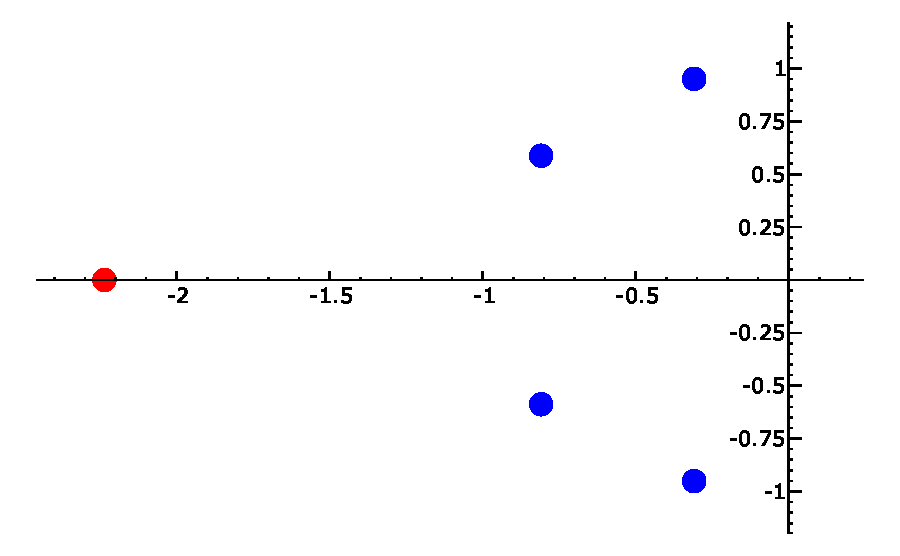
\includegraphics[width=\textwidth]{graphics/gauss_sum}
\caption{The red dot is the Gauss sum $g_2$ for $p=5$\label{fig:gauss_sum}}
\end{figure}

Figure~\ref{fig:gauss_sum} illustrates the Gauss sum $g_2$ for $p=5$.
The Gauss sum is obtained by adding the points on the unit circle,
with signs as indicated, to obtain the real number $-\sqrt{5}$.  This
suggests the following proposition, whose proof will require some
work.

\begin{proposition}[Gauss Sum]\label{prop:gauss_sum1}\iprop{Gauss sum}
For any~$a$ not divisible by~$p$,
$$
\ds g_a^2 = (-1)^{(p-1)/2}p.
$$
\end{proposition}

\begin{sg}
We illustrate using \sage that the proposition is
correct for $p=7$ and $p=13$:
%link
\begin{verbatim}
sage: [gauss_sum(a, 7)^2 for a in range(1,7)]
[-7, -7, -7, -7, -7, -7]
sage: [gauss_sum(a, 13)^2 for a in range(1,13)]
[13, 13, 13, 13, 13, 13, 13, 13, 13, 13, 13, 13]
\end{verbatim}
\end{sg}

In order to prove the proposition, we introduce a few lemmas.

\begin{lemma}\label{lem:gauss_sum1}
For any integer~$a$,
$$
\sum_{n=0}^{p-1} \zeta^{an} = \begin{cases}
        p & \text{\rm if $a \con 0\pmod{p}$,}\\
        0 & \text{\rm otherwise.}  \end{cases}
$$
\end{lemma}
\begin{proof}
If $a\con 0\pmod{p}$, then $\zeta^a=1$, so the sum equals the number of summands,
which is~$p$.  If $a\not\con 0\pmod{p}$, then we use the
identity $$x^p - 1 = (x-1)(x^{p-1} + \cdots + x + 1)$$ with $x = \zeta^a$. We have
 $\zeta^a\neq 1$, so $\zeta^a - 1 \neq 0$ and
$$
\sum_{n=0}^{p-1} \zeta^{an} = \frac{\zeta^{ap}-1}{\zeta^a-1} =
\frac{1-1}{\zeta^a-1} = 0.
$$
\end{proof}

\begin{lemma}\label{lem:gauss_sum2}
If $x$ and $y$ are arbitrary integers, then
$$
\sum_{n=0}^{p-1} \zeta^{(x-y)n} =
\begin{cases}
p & \text{\rm if $x\con y\pmod{p}$},\\
0 & \text{\rm otherwise}.
\end{cases}
$$
\end{lemma}
\begin{proof}
This follows from Lemma~\ref{lem:gauss_sum1} by
setting $a=x-y$.
\end{proof}


\begin{lemma}\label{lem:gauss_sum3}
We have $g_0=0$.
\end{lemma}
\begin{proof}
By definition
\begin{equation}\label{eqn:lem_gauss_3}
g_0 = \sum_{n=0}^{p-1} \kr{n}{p}.
\end{equation}
By Lemma~\ref{lem:qrhom}, the map
$$
\kr{\cdot}{p} : (\zmod{p})^* \ra \{\pm 1\}
$$
is a surjective homomorphism of groups.  Thus,  half the
elements of $(\zmod{p})^*$ map to $+1$ and half map to $-1$ (the
subgroup that maps to $+1$ has index $2$).  Since $\kr{0}{p}=0$, the
sum (\ref{eqn:lem_gauss_3}) is~$0$.
\end{proof}

\begin{lemma}\label{lem:gauss_sum4}
For any integer $a$,
$$
 g_a = \kr{a}{p}g_1.
$$
\end{lemma}
\begin{proof}
When $a\con 0\pmod{p}$, the lemma follows from
Lemma~\ref{lem:gauss_sum3}, so suppose that $a\not\con 0\pmod{p}$.  Then,
$$
\kr{a}{p} g_a = \kr{a}{p} \sum_{n=0}^{p-1} \kr{n}{p} \zeta^{an} = \sum_{n=0}^{p-1}\kr{an}{p} \zeta^{an} = \sum_{m=0}^{p-1}\kr{m}{p}\zeta^{m} = g_1.
$$
Here, we use that multiplication by $a$ is
an automorphism of $\zmod{p}$.  Finally, multiply both sides by
$\kr{a}{p}$ and use that $\kr{a}{p}^2=1$.
\end{proof}

\noindent{}We have enough lemmas to
prove Proposition~\ref{prop:gauss_sum1}.
\begin{proof}[Proof of Proposition~\ref{prop:gauss_sum1}]
We evaluate the sum $\sum_{a=0}^{p-1} g_a g_{-a}$ in two different ways.  By
Lemma~\ref{lem:gauss_sum4}, since $a\not\con 0\pmod{p}$ we have
$$
g_a g_{-a} = \kr{a}{p}g_1\kr{-a}{p}g_1 = \kr{-1}{p}\kr{a}{p}^2 g_1^2 = (-1)^{(p-1)/2} g_1^2,
$$
where the last step follows from Proposition~\ref{prop:euler}
and that $\kr{a}{p}\in\{\pm 1\}$.  Thus
\begin{equation}\label{eq:gauss_sum1_1}
 \sum_{a=0}^{p-1} g_a g_{-a} = (p-1)(-1)^{(p-1)/2}g_1^2.
\end{equation}
On the other hand, by definition
\begin{align*}
  g_a g_{-a} &= \sum_{n=0}^{p-1} \kr{n}{p}\zeta^{an} \cdot \sum_{m=0}^{p-1}\kr{m}{p}\zeta^{-am}\\
             &= \sum_{n=0}^{p-1}\sum_{m=0}^{p-1} \kr{n}{p}\kr{m}{p}\zeta^{an}\zeta^{-am}\\
             &= \sum_{n=0}^{p-1}\sum_{m=0}^{p-1} \kr{n}{p}\kr{m}{p}\zeta^{an-am}.
\end{align*}
Let $\delta(n,m)=1$ if $n\con m\pmod{p}$ and $0$ otherwise.
By Lemma~\ref{lem:gauss_sum2},
\begin{align*}
 \sum_{a=0}^{p-1} g_a g_{-a} &= \sum_{a=0}^{p-1}\sum_{n=0}^{p-1}\sum_{m=0}^{p-1} \kr{n}{p}\kr{m}{p}\zeta^{an-am}\\
            &= \sum_{n=0}^{p-1}\sum_{m=0}^{p-1} \kr{n}{p}\kr{m}{p}\sum_{a=0}^{p-1}\zeta^{an-am}\\
            &= \sum_{n=0}^{p-1}\sum_{m=0}^{p-1} \kr{n}{p}\kr{m}{p}p\delta(n,m)\\
            &= \sum_{n=0}^{p-1}\kr{n}{p}^2 p \\
            &= p(p-1).
\end{align*}
Equate (\ref{eq:gauss_sum1_1}) and the above equality,
then cancel $(p-1)$ to see that
$$
g_1^2 =(-1)^{(p-1)/2} p.
$$
Since $a\not\con 0\pmod{p}$, we have $\kr{a}{p}^2=1$, so by Lemma~\ref{lem:gauss_sum4},
$$
g_a^2 = \kr{a}{p}^2 g_1^2 = g_1^2,
$$
and the proposition is proved.
\end{proof}

\subsection{Proof of Quadratic Reciprocity}
We are now ready to prove Theorem~\ref{thm:recip} using
Gauss sums.
\begin{proof}
  Let~$q$ be an odd prime with $q\neq p$.  Set $p^* = (-1)^{(p-1)/2}p$
  and recall that Proposition~\ref{prop:gauss_sum1} asserts that $p^*
  = g^2$,
  where $g = g_1 = \sum_{n=0}^{p-1} \kr{n}{p}\zeta^n$.

  Proposition~\ref{prop:euler} implies that
  $$
  (p^*)^{(q-1)/2} \con \kr{p^*}{q} \pmod{q}.
  $$
  We have $g^{q-1} = (g^2)^{(q-1)/2} = (p^*)^{(q-1)/2}$, so
  multiplying both sides of the displayed equation by~$g$ yields a
  congruence
\begin{equation}\label{eqn:recip1}
  g^q \con g \kr{p^*}{q} \pmod{q}.
\end{equation}

But wait, what does this congruence mean, given that $g^q$ is not an
integer?  It means that the difference $g^q - g \kr{p^*}{q}$ is a
multiple of $q$ in the ring $\Z[\zeta]$ of all polynomials in $\zeta$
with coefficients in~$\Z$.


The ring $\Z[\zeta]/(q)$ has characteristic $q$, so
if~$x, y\in\Z[\zeta]$, then $(x+y)^q \con x^q + y^q \pmod{q}$.
Applying this to (\ref{eqn:recip1}), we see that
$$
g^q = \left(\sum_{n=0}^{p-1} \kr{n}{p}\zeta^n \right)^q \con \sum_{n=0}^{p-1} \kr{n}{p}^q \zeta^{nq} \con \sum_{n=0}^{p-1} \kr{n}{p} \zeta^{nq} \con g_q\pmod{q}.
$$
By Lemma~\ref{lem:gauss_sum4},
$$
g^q \con g_q \con \kr{q}{p} g\pmod{q}.
$$
Combining this with (\ref{eqn:recip1}) yields
$$
\kr{q}{p} g \con \kr{p^*}{q}g \pmod{q}.
$$
Since $g^2 = p^*$ and $p\neq q$, we can cancel~$g$ from both sides
to find that $\kr{q}{p} \con \kr{p^*}{q} \pmod{q}$.  Since both
residue symbols are $\pm 1$ and~$q$ is odd, it follows that $\kr{q}{p}
= \kr{p^*}{q}$.
Finally, we note using Corollary~\ref{cor:euler}
that
\begin{align*}
\kr{p^*}{q} &= \kr{(-1)^{(p-1)/2}p}{q}
        = \kr{-1}{q}^{(p-1)/2} \kr{p}{q}
        = \left(-1\right)^{\frac{q-1}{2}\cdot \frac{p-1}{2}} \cdot \kr{p}{q}.
\end{align*}
\end{proof}

\section{Finding Square Roots}\label{sec:findingsqrt}
\index{square roots!how to find mod $p$|(}\index{compute!square roots mod $p$|(}
We return in this section to the question of computing square roots.
If $K$ is a field in which $2\neq 0$, and $a,b,c\in K$, with $a\neq 0$,
then
the two solutions to the quadratic equation $ax^2+bx+c=0$ are
$$
x = \frac{-b\pm \sqrt{b^2-4ac}}{2a}.
$$
Now assume $K=\zmod{p}$, with~$p$ an odd prime.  Using
Theorem~\ref{thm:recip}, we can decide whether or not $b^2-4ac$ is a
perfect square in $\zmod{p}$, and hence whether or not $ax^2 + bx+c=0$
has a solution in $\zmod{p}$.  However,
Theorem~\ref{thm:recip} says nothing about how to actually find
a solution when there is one.
Also note that for this problem we do {\em not} need the
full Quadratic Reciprocity Law; in practice,
deciding whether an element of $\zmod{p}$ is
a perfect square with Proposition~\ref{prop:euler} is quite fast,
in view of Section~\ref{sec:arith_mod_n}.

Suppose $a\in \zmod{p}$ is a nonzero quadratic residue.
If $p\con 3 \pmod{4}$, then $b=a^{\frac{p+1}{4}}$
is a square root of~$a$ because
$$
  b^2 = a^{\frac{p+1}{2}} = a^{\frac{p-1}{2} + 1}
     = a^{\frac{p-1}{2}} \cdot a
          = \kr{a}{p} \cdot a = a.
$$
We can compute~$b$ in time polynomial in the number of digits of~$p$
using the powering algorithm of Section~\ref{sec:arith_mod_n}.


Suppose next that $p\con 1\pmod{4}$.
Unfortunately, we do not know a deterministic algorithm
that takes $a$ and $p$ as input, outputs
a square root of $a$ modulo $p$ when one exists,
and is polynomial-time in $\log(p)$.

\begin{remark}
  There is an algorithm due to Schoof \cite{schoof:sqrt} that computes
  the square root of $a$ in time $O((\sqrt(|a|)^{1/2 + \eps} \cdot
  \log(p))^9)$.  This beautiful algorithm (which makes use of elliptic
  curves) is not polynomial time in the sense described above, since
  for large $a$ it takes exponentially longer than for small $a$.
\end{remark}

We next describe a probabilistic algorithm to
compute a square root of~$a$ modulo $p$, which is very quick
in practice.
Recall the notion of ring from Definition~\ref{defn:ring}.
We will also need the notion of ring homomorphism and isomorphism.
\begin{definition}[Homomorphism of Rings]
Let $R$ and $S$ be rings.
A \defn{homomorphism of rings} $\vphi:R\to S$
is a map such that for all $a,b\in R$, we have
\begin{itemize}
\item $\vphi(ab) =\vphi(a)\vphi(b)$,
\item $\vphi(a+b) = \vphi(a) + \vphi(b)$, and
\item $\vphi(1) = 1$.
\end{itemize}
An \defn{isomorphism} $\vphi:R\to S$ of rings is a
ring homomorphism that is bijective.
\end{definition}

Consider the ring
$$R = (\zmod{p})[x]/(x^2 - a)$$
defined as follows.
We have
$$
R = \{ u + v \alpha : u, v \in \zmod{p}\}
$$
with multiplication defined by
$$
(u+v\alpha)(z+w\alpha) = (uz + awv) + (uw+vz)\alpha.
$$
Here $\alpha$ corresponds to the class of $x$ in $R$.
\begin{sg}
We define and work with the ring $R$ above
in \sage as follows (for $p=13$):
\begin{verbatim}
sage: S.<x> = PolynomialRing(GF(13))
sage: R.<alpha> = S.quotient(x^2 - 3)
sage: (2+3*alpha)*(1+2*alpha)
7*alpha + 7
\end{verbatim}
\end{sg}


Let $b$ and~$c$ be the square roots of~$a$ in $\zmod{p}$
(though we cannot easily
compute~$b$ and~$c$ yet, we can consider them in order
to deduce an algorithm to find them).
We have ring homomorphisms
$f:R\to \zmod{p}$ and $g:R\to \zmod{p}$
given by $f(u+v\alpha) = u+vb$ and $g(u+v\alpha) = u + vc$.
Together, these define a ring isomorphism
$$
  \vphi : R \lra \zmod{p} \cross \zmod{p}
$$
given by $\vphi(u+v\alpha) = (u+vb,u+vc)$.
Choose in some way a random element~$z$ of $(\zmod{p})^*$, and
define $u,v\in\zmod{p}$ by
$$
u+v\alpha = (1+z\alpha)^{\frac{p-1}{2}},
$$
where we compute $(1+z\alpha)^{\frac{p-1}{2}}$ quickly
using an analog of the
binary powering algorithm of Section~\ref{sec:compute_powers}.
If $v=0$, we try again with another random~$z$.  If $v\neq 0$, we can
quickly find the desired square roots~$b$ and~$c$ as follows.  The
quantity $u+vb$ is a $(p-1)/2$ power in $\zmod{p}$, so it equals
either $0$, $1$, or $-1$, so $b = -u/v$, $(1-u)/v$, or $(-1-u)/v$,
respectively.  Since we know~$u$ and~$v$, we can try each of $-u/v$,
$(1-u)/v$, and $(-1-u)/v$ and see which is a square root of~$a$.

\begin{example}\label{ex:69sqrt}
Continuing Example~\ref{ex:69},
we find a square root of~$69$ modulo~$389$.
We apply the algorithm described above in the case $p\con 1\pmod{4}$.
We first choose the random $z=24$ and find that
$
 (1+24\alpha)^{194} = -1.
$
The coefficient of~$\alpha$ in the power is~$0$, and we try again with
$z=51$.
This time, we have $(1+51\alpha)^{194} = 239\alpha = u +v\alpha$.
The inverse of $239$ in $\zmod{389}$ is $153$, so we consider the
following three possibilities for a square root of~$69$:
$$
  -\frac{u}{v} = 0 \qquad
  \frac{1-u}{v} = 153\qquad
  \frac{-1-u}{v} = -153.
$$
Thus, $153$ and $-153$ are the square roots of $69$ in $\zmod{389}$.
\end{example}

\begin{sg}
We implement the above algorithm in \sage and illustrate it
with some examples.
\begin{verbatim}
sage: def find_sqrt(a, p):
...    assert (p-1)%4 == 0
...    assert legendre_symbol(a,p) == 1
...    S.<x> = PolynomialRing(GF(p))
...    R.<alpha> = S.quotient(x^2 - a)
...    while True:
...        z = GF(p).random_element()
...        w = (1 + z*alpha)^((p-1)//2)
...        (u, v) = (w[0], w[1])
...        if v != 0: break
...    if (-u/v)^2 == a: return -u/v
...    if ((1-u)/v)^2 == a: return (1-u)/v
...    if ((-1-u)/v)^2 == a: return (-1-u)/v
...
sage: b = find_sqrt(3,13)
sage: b                        # random: either 9 or 3
9
sage: b^2
3
sage: b = find_sqrt(3,13)
sage: b                        # see, it's random
4
sage: find_sqrt(5,389)         # random: either 303 or 86
303
sage: find_sqrt(5,389)         # see, it's random
86
\end{verbatim}
\end{sg}



\index{square roots!how to find mod $p$|)}\index{compute!square roots mod $p$|)}


%%%%%%%%%%%%%%%%%%%%%%%%%%%%%%%%%%%%%%%%%%%%%%%%%%%%%%%%%%%%%%%%%%




\begin{exercises}
\item\label{ex:rec1} Calculate the following by hand:
  $\kr{3}{97}$, $\kr{3}{389}$, $\kr{22}{11}$, and $\kr{5!}{7}$.

\item \label{ex:powering} Let $G$ be an abelian group,
and let $n$ be a positive integer.
\begin{enumerate}
\item Prove that the
map $\vphi:G\to G$ given by $\vphi(x) = x^n$ is a group
homomorphism.
\item Prove that the subset $H$ of $G$ of squares
of elements of $G$ is a subgroup.
\end{enumerate}

\item\label{ex:rec2} Use Theorem~\ref{thm:recip}
to show that for $p\geq 5$ prime,
  $$ \kr{3}{p} = \begin{cases} \hfill 1 & \text{ if }p\con 1, 11\pmod{12},\\
    -1 & \text{ if }p\con 5, 7\pmod{12}.  \end{cases}$$

\item\label{ex:rec5}(*) Use that $(\zmod{p})^*$ is cyclic to give a
  direct proof that $\kr{-3}{p}=1$ when $p\con 1\pmod{3}$. (Hint:
  There is an element $c\in (\zmod{p})^*$ of order~$3$.  Show that
  $(2c+1)^2=-3$.)


\item\label{ex:rec6}(*) If $p\con 1\pmod{5}$, show directly that
  $\kr{5}{p}=1$ by the method of \exref{ch:reciprocity}{ex:rec5}.
  (Hint: Let $c\in(\zmod{p})^*$ be an element of order~$5$.  Show that
  $(c+c^4)^2+(c+c^4)-1=0$, etc.)

%\item\label{ex:rec7} For which odd primes~$p$ is $\ds \sum_{a=1}^{p-1}
%  \kr{a}{p}=0$?

\item\label{ex:rec8} (*) Let $p$ be an odd prime. In this exercise, you
  will prove that $\kr{2}{p}=1$ if and only if $p\con
  \pm 1\pmod{8}$.
\begin{enumerate}
\item Prove that
$$
  x = \frac{1-t^2}{1+t^2}, \qquad y = \frac{2t}{1+t^2}
$$
is a parameterization of the set of solutions to $x^2+y^2\con 1\pmod{p}$,
in the sense that the solutions $(x,y)\in \zmod{p} \times \zmod{p}$ are in
bijection with the $t\in \zmod{p} \union\{\infty\}$ such that $1+t^2\not\con 0\pmod{p}$.
Here, $t=\infty$ corresponds to the point $(-1,0)$.
(Hint: if $(x_1,y_1)$ is a solution, consider the line $y=t(x+1)$
through $(x_1,y_1)$ and $(-1,0)$, and solve for $x_1, y_1$ in terms
of $t$.)
\item Prove that the number of solutions to $x^2+y^2\con 1\pmod{p}$
is $p+1$ if $p\con 3\pmod{4}$ and $p-1$ if $p\con 1\pmod{4}$.
\item Consider the set $S$ of pairs $(a,b)\in (\zmod{p})^*\times (\zmod{p})^*$ such
that $a+b=1$ and $\kr{a}{p}=\kr{b}{p}=1$.  Prove that
$\#S=(p+1-4)/4$ if $p\con 3\pmod{4}$ and $\#S = (p-1-4)/4$
if $p\con 1\pmod{4}$.  Conclude that $\#S$ is odd if and only if
$p\con \pm 1\pmod{8}$.
\item The map $\sigma(a,b)=(b,a)$ that swaps coordinates is a
  bijection of the set $S$. It has exactly one fixed point if and
  only if there is an $a\in\zmod{p}$ such that $2a=1$ and $\kr{a}{p}=1$.
  Also, prove that $2a=1$ has a solution $a\in\zmod{p}$ with $\kr{a}{p}=1$
if and only if $\kr{2}{p}=1$.
\item Finish by showing that $\sigma$ has exactly one fixed point
if and only if $\#S$ is odd, i.e., if and only if
$p\con \pm 1\pmod{8}$.
\end{enumerate}
Remark: The method of proof of this exercise can be generalized to give a
proof of the full Quadratic Reciprocity Law.

\item\label{ex:rec9} How many natural numbers $x < 2^{13}$ satisfy the
  equation
  $$
  x^2\con 5\pmod{2^{13}-1}? $$
  You may assume that $2^{13}-1$ is prime.

\item\label{ex:rec10} Find the natural number $x<97$ such that $x\con
  4^{48}\pmod{97}$.  Note that $97$ is prime.


\item\label{ex:rec13} In this problem, we will formulate an analog of
  quadratic reciprocity for a symbol like $\kr{a}{q}$, but without the
  restriction that~$q$ be a prime.  Suppose $n$ is an odd positive integer,
  which we factor as $\prod_{i=1}^k p_i^{e_i}$.  We
  define the Jacobi symbol $\kr{a}{n}$ as follows:
  $$
  \kr{a}{n} = \prod_{i=1}^k \kr{a}{p_i}^{e_i}.
  $$
\begin{enumerate}
\item Give an example to show that $\kr{a}{n}=1$ need not imply that
  $a$ is a perfect square modulo $n$.
\item (*) Let $n$ be odd and $a$ and $b$ be integers.  Prove that the
  following holds:
\begin{enumerate}
\item $\kr{a}{n}\kr{b}{n} = \kr{ab}{n}$. (Thus $a\mapsto \kr{a}{n}$
  induces a homomorphism from $(\zmod{n})^*$ to $\{\pm 1\}$.)
\item $\kr{-1}{n} \con n \pmod{4}$.
\item $\kr{2}{n}=1$ if $n\con \pm 1\pmod{8}$ and $-1$ otherwise.
\item Assume $a$ is positive and odd.  Then $\kr{a}{n} =
  (-1)^{\frac{a-1}{2} \cdot \frac{n-1}{2}} \kr{n}{a}$
\end{enumerate}
\end{enumerate}

\item\label{ex:rec14}(*) Prove that for any $n\in\Z$, the integer
  $n^2+n+1$ does not have any divisors of the form $6k-1$.

\end{exercises}


%%%%%%%%%%%%%%%%%%%%%%%%%%%%%%%%%%%%%%%%%%%%%%%%%%%%%%%%%%%%%%%%%%%%%%%
%%
%% Chapter: Continued Fractions
%%
%%%%%%%%%%%%%%%%%%%%%%%%%%%%%%%%%%%%%%%%%%%%%%%%%%%%%%%%%%%%%%%%%%%%%%%

\chapter{Continued Fractions}\label{ch:contfrac}

The golden ratio
$\frac{1+\sqrt{5}}{2}$ is
equal to the infinite fraction
$$
1+ \frac{\displaystyle 1}{\displaystyle 1+ \frac{\displaystyle 1}{\displaystyle 1 +
\frac{1}{1 + \cdots,}}}
$$
and the fraction
$$
\frac{103993}{33102}=3.14159265301190260407\ldots
$$
is an excellent approximation to $\pi$.
Both of these observations are explained by continued fractions.

Continued fractions are theoretically beautiful and provide tools
that yield powerful algorithms for solving problems in number theory.
For example, continued fractions provide a fast way to write a
prime---even a hundred digit prime---as a sum of two squares, when
possible.

Continued fractions are thus a beautiful algorithmic and conceptual tool
in number theory that has many applications.  For example, they
provide a surprisingly efficient way to recognize a rational number
given just the first few digits of its decimal expansion, and they
give a sense in which~$e$ is ``less complicated'' than~$\pi$ (see
Example~\ref{ex:e_and_pi} and Section~\ref{sec:contfrac_e}).


In Section~\ref{sec:finitecontfrac}, we study continued fractions of
finite length and lay the foundations for our later investigations.
In Section~\ref{sec:cfinfty}, we give the continued fraction procedure,
which associates to a real number~$x$ a continued fraction that
converges to $x$.  In Section~\ref{sec:cfqi}, we characterize
(eventually) periodic continued fractions as the continued fractions
of nonrational roots of quadratic polynomials, then discuss an
unsolved mystery concerning continued fractions of roots of
irreducible polynomials of degree greater than~$2$.  We conclude the
chapter with applications of continued fractions to recognizing
approximations to rational numbers (Section~\ref{sec:cf_rat}) and
writing integers as sums of two squares (Section~\ref{sec:sumsqr}).

The reader is encouraged to read more about continued fractions
in \cite[Ch.~X]{hardywright}, \cite{khintchine},
\cite[\S13.3]{burton}, and \cite[Ch.~7]{niven-zuckerman-montgomery}.

\section{The Definition}
A \defn{continued fraction}\index{continued fraction|(}
is an expression of the form
$$
  a_0 + \frac{1}{\ds a_1+\frac{1}{\ds a_2+\frac{1}{\ds a_3+\cdots.}}}
$$

In this book, we will assume that the $a_i$ are real numbers and
$a_i>0$ for $i\geq 1$, and the expression may or may not go on
indefinitely.  More general notions of continued fractions have been
extensively studied, but they are beyond the scope of this book.
We will be most interested in the case when the $a_i$ are all
integers.

We denote the continued fraction displayed above by
$$
  [a_0,a_1,a_2,\ldots].
$$
For example,
$$[1,2] = 1+\frac{1}{2} = \frac{3}{2},$$
\begin{align*}
[3, 7, 15, 1, 292 ] &= 3 + \frac{1}{\ds 7+ \frac{1}{\ds 15+\frac{1}{\ds 1+\frac{1}{292}}}}\\
 &= \frac{103993}{33102}=3.14159265301190260407\ldots,
\end{align*}
and
\begin{align*}
[2, 1, 2, 1, 1, 4, 1, 1, 6] &=
  2 + \frac{1}{\ds 1 +\frac{1}{\ds 2 +\frac{1}{\ds 1 + \frac{1}{\ds 1 + \frac{1}{\ds 4 + \frac{1}{\ds 1 + \frac{1}{\ds 1 + \frac{1}{\ds 6}}}}}}}} \\
  &= \frac{1264}{465} \\
  &= 2.7182795698924731182795698\ldots
\end{align*}
The second two examples were chosen to foreshadow that continued
fractions can be used to obtain good rational approximations to
irrational numbers.  Note that the first approximates~$\pi$,
and the second~$e$.



\section{Finite Continued Fractions}\label{sec:finitecontfrac}
This section is about continued fractions of
the form $[a_0,a_1,\ldots, a_m]$ for some $m\geq 0$.
We give an inductive definition of numbers $p_n$ and $q_n$
such that for all $n\leq m$
\begin{equation}\label{eqn:quocontfrac}
  [a_0,a_1,\ldots,a_n] = \frac{p_n}{q_n}.
\end{equation}
We then give related formulas for
the determinants of the $2\times 2$
matrices $\abcd{p_n}{p_{n-1}}{q_n}{q_{n-1}}$ and
$\abcd{p_n}{p_{n-2}}{q_n}{q_{n-2}}$,  which we will repeatedly use to
deduce properties of the sequence of partial convergents
$[a_0,\ldots,a_k]$.
We will use Algorithm~\ref{alg:gcd} to prove that every
rational number is represented by a continued fraction, as in
(\ref{eqn:quocontfrac}).

\begin{definition}[Finite Continued Fraction]
\index{continued fraction!of finite length|nn}\index{finite continued fraction|nn}
A \defn{finite continued fraction} is an expression
$$
    a_0 + \frac{1}{\ds a_1+\frac{1}{\ds a_2 +
         \ds \frac{1}{ \cdots +\frac{1}{a_n}}}}
$$
where each $a_m$ is a real number and $a_m>0$ for all $m\geq 1$.
\end{definition}

\begin{definition}[Simple Continued Fraction]
A \defn{simple continued fraction} is a finite or infinite continued
fraction in which the $a_i$ are all integers.
\end{definition}

To get a feeling for continued fractions, observe that
\begin{align*}
[a_0] &= a_0,\\
[a_0, a_1] &= a_0 + \frac{1}{a_1} = \frac{a_0 a_1 + 1}{a_1},\\
[a_0, a_1, a_2] &= a_0 + \frac{1}{a_1 +\ds \frac{1}{a_2}}
            = \frac{a_0 a_1 a_2 + a_0 + a_2}{a_1 a_2 + 1}.
\end{align*}
Also,
\begin{align*}
  [a_0, a_1, \ldots ,a_{n-1}, a_n] &=
          \left[a_0, a_1, \ldots, a_{n-2}, a_{n-1} + \frac{1}{a_n}\right]\\
        &= a_0 + \frac{1}{[a_1,\ldots, a_n]} \\
        &= [a_0, [a_1,\ldots, a_n]].
\end{align*}

\begin{sg}
The \code{continued\_fraction} command  computes
continued fractions:
\begin{verbatim}
sage: continued_fraction(17/23)
[0, 1, 2, 1, 5]
sage: continued_fraction(e)
[2, 1, 2, 1, 1, 4, 1, 1, 6, 1, 1, 8, 1, 1, 10, 1, 1,
 12, 1, 1]
\end{verbatim}
Use the optional second argument \code{bits = n} to determine the
precision (in bits) of the input number that is used to compute the
continued fraction.
\begin{verbatim}
sage: continued_fraction(e, bits=21)
[2, 1, 2, 1, 1, 4, 1, 1, 6]
sage: continued_fraction(e, bits=30)
[2, 1, 2, 1, 1, 4, 1, 1, 6, 1, 1, 8]
\end{verbatim}
You can obtain the value of a continued fraction
and even do arithmetic with continued fractions:
\begin{verbatim}
sage: a = continued_fraction(17/23); a
[0, 1, 2, 1, 5]
sage: a.value()
17/23
sage: b = continued_fraction(6/23); b
[0, 3, 1, 5]
sage: a + b
[1]
\end{verbatim}
\end{sg}

\subsection{Partial Convergents}\label{sec:partconv}
\index{partial convergents|nn}\index{continued fraction!partial convergents of|nn}%
Fix a finite continued fraction $[a_0,\ldots,a_m]$.  We do not assume
at this point that the $a_i$ are integers.

\begin{definition}[Partial convergents]
For $0\leq n\leq m$, the $n$th \defn{convergent} of the
continued fraction $[a_0,\ldots,a_m]$
is $[a_0,\ldots, a_n]$.  These convergents for $n<m$ are
also called \defn{partial convergents}.
\end{definition}

For each $n$ with $-2\leq n\leq m$,
define real numbers $p_n$ and $q_n$ as follows:
$$\begin{array}{lllcl}
  p_{-2}=0, & \quad p_{-1} = 1, & \quad  p_0 = a_0,\quad
                &\cdots &\,\,p_n = a_n p_{n-1} + p_{n-2} \quad \cdots,\\
  q_{-2}=1, & \quad q_{-1} = 0, &\quad q_0 = 1, \quad
                &\cdots &\,\,q_n = a_n q_{n-1} + q_{n-2} \quad \cdots.
\end{array}
$$

\begin{proposition}[Partial Convergents]\label{prop:convergents}%
\iprop{partial convergents}
For $n\geq 0$ with $n\leq m$ we have $$ [a_0, \ldots, a_n] = \frac{p_n}{q_n}.$$
\end{proposition}
\begin{proof}
We use induction.  The assertion is obvious when $n=0,1$.  Suppose the
proposition is true for all continued fractions of length $n-1$.  Then
\begin{align*}
[a_0,\ldots, a_n]
 &= [a_0,\ldots,a_{n-2}, a_{n-1} + \frac{1}{a_n}]\\
 &= \frac{\left( a_{n-1} + \frac{1}{a_n}\right) p_{n-2} + p_{n-3}}
         {\left( a_{n-1} + \frac{1}{a_n}\right) q_{n-2} + q_{n-3}}\\
 &= \frac{(a_{n-1}a_n +1)p_{n-2} + a_n p_{n-3}}
         {(a_{n-1}a_n +1)q_{n-2} + a_n q_{n-3}}\\
 &= \frac{a_n(a_{n-1}p_{n-2} + p_{n-3}) + p_{n-2}}
         {a_n(a_{n-1}q_{n-2} + q_{n-3}) + q_{n-2}}\\
 &= \frac{a_n p_{n-1} + p_{n-2}}{a_n q_{n-1} + q_{n-2}}\\
 &= \frac{p_n}{q_n}.
\end{align*}
\end{proof}
\begin{sg}
If \code{c} is a continued fraction, use \code{c.convergents()}
to compute a list of the partial
convergents of \code{c}.
\begin{verbatim}
sage: c = continued_fraction(pi,bits=35); c
[3, 7, 15, 1, 292, 1]
sage: c.convergents()
[3, 22/7, 333/106, 355/113, 103993/33102, 104348/33215]
\end{verbatim}
As we will see, the convergents of a continued fraction
are the best rational approximations to the value of
the continued fraction.  In the example above, the
listed convergents are the best rational approximations
of $\pi$ with given denominator size.
\end{sg}

\begin{proposition}\label{prop:dets}
For $n\geq 0$ with $n\leq m$ we have
\begin{equation}\label{eqn:detsign}
p_n q_{n-1} - q_n p_{n-1} = (-1)^{n-1}
\end{equation}
and
\begin{equation}\label{eqn:detsignan}
p_nq_{n-2} - q_n p_{n-2} = (-1)^n a_n.
\end{equation}
Equivalently,
$$\frac{p_n}{q_n} - \frac{p_{n-1}}{q_{n-1}} =
                  (-1)^{n-1}\cdot\frac{1}{q_n q_{n-1}}$$
and
$$\frac{p_n}{q_n} - \frac{p_{n-2}}{q_{n-2}} =
                  (-1)^{n}\cdot\frac{a_n}{q_n q_{n-2}}.$$
\end{proposition}
\begin{proof}
The case for $n=0$ is obvious from the definitions.
Now suppose $n>0$ and the statement is true for $n-1$.  Then
\begin{align*}
p_{n}q_{n-1} - q_n p_{n-1} &=
     (a_n p_{n-1} + p_{n-2}) q_{n-1} - (a_n q_{n-1} + q_{n-2}) p_{n-1}\\
  &= p_{n-2}q_{n-1} - q_{n-2} p_{n-1} \\
   &=
       -(p_{n-1}q_{n-2} - p_{n-2} q_{n-1})\\
  &= -(-1)^{n-2} = (-1)^{n-1}.
\end{align*}
This completes the proof of (\ref{eqn:detsign}).  For
(\ref{eqn:detsignan}), we have
\begin{align*}
p_n q_{n-2} - p_{n-2} q_n &=
        (a_n p_{n-1} + p_{n-2})q_{n-2} - p_{n-2}(a_n q_{n-1} + q_{n-2}) \\
       &= a_n(p_{n-1}q_{n-2} - p_{n-2}q_{n-1}) \\
       &= (-1)^n a_n.
\end{align*}
\end{proof}

\begin{remark}
Expressed in terms of matrices, the proposition asserts that the determinant
of  $\abcd{p_n}{p_{n-1}}{q_n}{q_{n-1}}$ is
$(-1)^{n-1}$, and of
$\abcd{p_n}{p_{n-2}}{q_n}{q_{n-2}}$ is  $(-1)^{n}a_n$.
\end{remark}

\begin{sg}
We use \sage to verify Proposition~\ref{prop:dets}
for the first few terms of the continued
fraction of $\pi$.
\begin{verbatim}
sage: c = continued_fraction(pi); c
[3, 7, 15, 1, 292, 1, 1, 1, 2, 1, 3, 1, 14]
sage: for n in range(-1, len(c)):
...    print c.pn(n)*c.qn(n-1) - c.qn(n)*c.pn(n-1),
1 -1 1 -1 1 -1 1 -1 1 -1 1 -1 1 -1
sage: for n in range(len(c)):
...    print c.pn(n)*c.qn(n-2) - c.qn(n)*c.pn(n-2),
3 -7 15 -1 292 -1 1 -1 2 -1 3 -1 14
\end{verbatim}
\end{sg}

\begin{corollary}[Convergents in lowest terms]\icor{convergents in lowest terms}%
\label{cor:lowest}
If $[a_0,a_1,\ldots,a_m]$ is a simple continued fraction,
so each $a_i$ is an integer,
then the $p_n$ and $q_n$ are integers and
the fraction $p_n/q_n$ is in lowest terms.
\end{corollary}
\begin{proof}
  It is clear that the $p_n$ and $q_n$ are integers, from the formula
  that defines them.  If~$d$ is a positive divisor of both $p_n$ and
  $q_n$, then $d\mid (-1)^{n-1}$, so $d=1$.
\end{proof}

\begin{sg}
We illustrate Corollary~\ref{cor:lowest} using \sage.
\begin{verbatim}
sage: c = continued_fraction([1,2,3,4,5])
sage: c.convergents()
[1, 3/2, 10/7, 43/30, 225/157]
sage: [c.pn(n) for n in range(len(c))]
[1, 3, 10, 43, 225]
sage: [c.qn(n) for n in range(len(c))]
[1, 2, 7, 30, 157]
\end{verbatim}
\end{sg}

\subsection{The Sequence of Partial Convergents}\index{convergents!partial}
\index{continued fraction!convergents}
Let $[a_0,\ldots, a_m]$ be a continued fraction and for
$n\leq m$ let
$$
  c_n = [a_0, \ldots, a_n] = \frac{p_n}{q_n}
$$
denote the $n$th convergent.  Recall that by definition of continued
fraction, $a_n>0$ for $n>0$, which gives the partial convergents of a
continued fraction additional structure.  For example, the partial
convergents of $[2, 1, 2, 1, 1, 4, 1, 1, 6]$ are
$$
2, 3, 8/3, 11/4, 19/7, 87/32, 106/39, 193/71, 1264/465.
$$
To make the size of these numbers clearer, we approximate
them using decimals.  We also underline every other number,
to illustrate some extra structure.
$$
 \underline{2}, 3,  \underline{2.66667}, 2.75000,  \underline{2.71429},
2.71875,  \underline{2.71795}, 2.71831,  \underline{2.71828}
$$
The underlined numbers are smaller than all of the
nonunderlined numbers, and the sequence of underlined numbers is
strictly increasing, whereas the nonunderlined numbers strictly
decrease.
\begin{sg}
  Figure~\ref{fig:cf} illustrates the above pattern on
  another continued fraction using \sage.
\begin{verbatim}
sage: c = continued_fraction([1,1,1,1,1,1,1,1])
sage: v = [(i, c.pn(i)/c.qn(i)) for i in range(len(c))]
sage: P = point(v, rgbcolor=(0,0,1), pointsize=40)
sage: L = line(v, rgbcolor=(0.5,0.5,0.5))
sage: L2 = line([(0,c.value()),(len(c)-1,c.value())], \
...      thickness=0.5, rgbcolor=(0.7,0,0))
sage: (L+L2+P).show(xmin=0,ymin=1)
\end{verbatim}
\end{sg}
\begin{figure}
\begin{center}
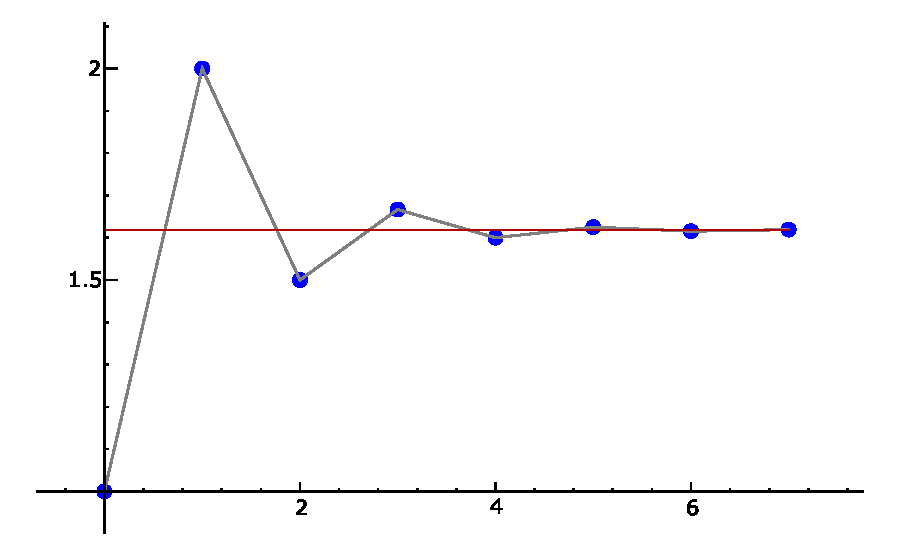
\includegraphics[width=0.8\textwidth]{graphics/cfbounce}
\end{center}
\caption{Graph of a Continued Fraction\label{fig:cf}}
\end{figure}

We next prove that this extra structure is a general
phenomenon.

\begin{proposition}[How Convergents Converge]\label{prop:conv_incdec}%
\iprop{how convergents converge}%
The even indexed convergents $c_{2n}$ increase strictly with~$n$, and the
odd indexed convergents $c_{2n+1}$ decrease strictly with~$n$.  Also,
the odd indexed convergents $c_{2n+1}$ are greater than all of the
even indexed convergents $c_{2m}$.
\end{proposition}
\begin{proof}
The $a_n$ are positive for $n\geq 1$, so the $q_n$ are positive.
By Proposition~\ref{prop:dets}, for $n\geq 2$,
$$c_n - c_{n-2} = (-1)^n \cdot \frac{a_n}{q_n q_{n-2} },$$
which proves the first claim.

Suppose for the sake of contradiction that there exist
integers $r$ and $m$ such that $c_{2m+1} < c_{2r}$.
Proposition~\ref{prop:dets} implies that for $n\geq 1$,
$$
c_n - c_{n-1} = (-1)^{n-1}\cdot \frac{1}{q_n q_{n-1}}
$$
has sign $(-1)^{n-1}$, so for all $s\geq 0$ we have $c_{2s+1} >
c_{2s}$.  Thus it is impossible that $r= m$.  If $r<m$, then by
what we proved in the first paragraph,
$c_{2m+1} < c_{2r} < c_{2m}$, a contradiction (with $s=m$).  If $r>m$, then
$c_{2r+1} < c_{2m+1} < c_{2r}$, which is also a contradiction (with $s=r$).
\end{proof}


\subsection{Every Rational Number is Represented}
\index{continued fraction!every rational number has}
\begin{proposition}[Rational Continued Fractions]%
\label{prop:ratcf}\iprop{rational continued fractions}%
  Every nonzero rational number can be represented by a simple
  continued fraction.
\end{proposition}
\begin{proof}
Without loss of generality, we may assume that the rational
number is $a/b$, with $b\geq 1$ and $\gcd(a,b)=1$.
Algorithm~\ref{alg:gcd} gives:
\begin{align*}
a &= b\cdot a_0 + r_1, & 0<r_1<b\\
b &= r_1\cdot a_1 + r_2, & 0<r_2<r_1\\
 &\cdots &\\
r_{n-2} &= r_{n-1}\cdot a_{n-1} + r_n, & 0<r_n < r_{n-1}\\
r_{n-1} &= r_n\cdot a_n + 0.
\end{align*}
Note that $a_i>0$ for $i>0$ (also $r_n=1$, since $\gcd(a,b)=1$).
Rewrite the equations as follows:
\begin{align*}
a/b &= a_0 + r_1/b = a_0 + 1/(b/r_1),\\
b/r_1 &= a_1 + r_2 / r_1 = a_1 + 1/(r_1/r_2),\\
r_1/r_2 &= a_2 + r_3 / r_2 = a_2 + 1/(r_2/r_3),\\
\cdots\\
r_{n-1}/r_n &= a_n.
\end{align*}
It follows that
$$
   \frac{a}{b} = [a_0,a_1,\ldots, a_n].
$$
\end{proof}

The proof of Proposition~\ref{prop:ratcf} leads to an algorithm
for computing the continued fraction of a rational number.
%See Section~\ref{sec:comp_contfrac} for an implementation.

A nonzero rational number can be represented in exactly two ways;
for example, $2=[1,1] = [2]$ (see \exref{ch:contfrac}{ex:cf3b}).


\section{Infinite Continued Fractions}\label{sec:cfinfty}
\index{compute!continued fraction}
This section begins with the continued fraction procedure, which associates
a sequence $a_0,a_1,\ldots$ of integers to a real number~$x$.  After
giving several examples, we prove that $x = \lim_{n\ra\infty}
[a_0,a_1,\ldots,a_n]$ by proving that the odd and even partial
convergents become arbitrarily close to each other.
We also show that if $a_0,a_1,\ldots$ is any infinite
sequence of positive integers, then the sequence of
$c_n=[a_0,a_1,\ldots,a_n]$
converges. More generally, if $a_n$ is an arbitrary sequence
of positive reals
such that $\sum_{n=0}^{\infty} a_n$ diverges then $(c_n)$ converges.

\subsection{The Continued Fraction Procedure}
\index{continued fraction!algorithm}\label{sec:cfalg}
Let $x\in\R$ and write
  $$x = a_0 + t_0$$
with $a_0\in\Z$ and $0\leq t_0 < 1$.
We call the number $a_0$ the \defn{floor} of~$x$, and
we also sometimes write $a_0 = \lfloor x \rfloor$.
If $t_0\neq 0$, write
$$\frac{1}{t_0} = a_1 + t_1$$ with $a_1\in\N$ and $0\leq t_1 < 1$.
Thus $t_0 = \frac{1}{a_1 + t_1}=[0,a_1+t_1]$, which is a
continued fraction expansion of $t_0$, which need not be simple.
Continue in this manner so long as $t_n\neq 0$ writing
$$
  \frac{1}{t_n} = a_{n+1} + t_{n+1}
$$
with $a_{n+1}\in\N$ and $0\leq t_{n+1}<1$.
We call this procedure, which associates to a real number~$x$ the sequence
of integers $a_0, a_1, a_2, \ldots $, the
\defn{continued fraction process}.

\begin{example}
Let $x=\frac{8}{3}$.  Then $x=2+\frac{2}{3}$, so
$a_0=2$ and $t_0=\frac{2}{3}$.  Then
$\frac{1}{t_0}=\frac{3}{2} = 1+\frac{1}{2}$, so $a_1=1$ and $t_1=\frac{1}{2}$.
Then $\frac{1}{t_1} = 2$, so $a_2=2$, $t_2=0$, and the sequence terminates.
Notice that
$$ \frac{8}{3} = [2,1,2],$$
so the continued fraction procedure produces the
continued fraction of $\frac{8}{3}$.
\end{example}



\begin{example}\label{cf:golden}
Let $x = \frac{1+\sqrt{5}}{2}.$  Then
$$
   x = 1 + \frac{-1 + \sqrt{5}}{2},
$$
so $a_0 = 1$ and $t_0 = \frac{-1+\sqrt{5}}{2}$.
We have
$$
  \frac{1}{t_0} = \frac{2}{-1+\sqrt{5}} = \frac{-2-2\sqrt{5}}{-4}
        = \frac{1+\sqrt{5}}{2},
$$
so $a_1 = 1$ and $t_1 =  \frac{-1+\sqrt{5}}{2}$.
Likewise, $a_n = 1$ for all~$n$.
As we will see below, the following exciting
equality makes sense.
$$\frac{1+\sqrt{5}}{2} =
1 + \frac{1}{\ds 1 + \frac{1}{\ds 1 + \frac{1}{\ds 1 + \frac{1}{\ds 1 + \frac{1}{\ds 1 + \cdots}}}}}
$$
\end{example}
\begin{sg}
The equality of Example~\ref{cf:golden}
is consistent with the following \sage calculation:
\begin{verbatim}
sage: def cf(bits):
...   x = (1 + sqrt(RealField(bits)(5))) / 2
...   return continued_fraction(x)
sage: cf(10)
[1, 1, 1, 1, 1, 1, 1]
sage: cf(30)
[1, 1, 1, 1, 1, 1, 1, 1, 1, 1, 1, 1, 1, 1, 1, 1, 1, 1,
 1, 1, 1]
sage: cf(50)
[1, 1, 1, 1, 1, 1, 1, 1, 1, 1, 1, 1, 1, 1, 1, 1, 1, 1,
 1, 1, 1, 1, 1, 1, 1, 1, 1, 1, 1, 1, 1, 1, 1, 1, 1, 1]
\end{verbatim}
\end{sg}

\begin{example}\label{ex:e_and_pi}\index{continued fraction!of $e$}
Suppose $x = e = 2.71828182\ldots$.  Using the continued
fraction procedure, we find that
$$
 a_0, a_1, a_2, \ldots = 2,1,2,1,1,4,1,1,6,1,1,8,1,1,10,\ldots
$$
For example,
$a_0=2$ is the floor of $2$.  Subtracting $2$ and inverting,
we obtain
$1/0.718\ldots  = 1.3922\ldots$, so $a_1=1$.  Subtracting $1$
and inverting yields $1/0.3922\ldots = 2.5496\ldots$, so
$a_2=2$.  We will prove in Section~\ref{sec:contfrac_e} that the
continued fraction of~$e$ obeys a simple pattern.

The $5$th partial convergent of the continued fraction of~$e$ is
$$
[a_0,a_1,a_2,a_3,a_4,a_5] = \frac{87}{32} = 2.71875,
$$
which is a good rational approximation to~$e$, in the
sense that $$\abs{\frac{87}{32} - e} = 0.000468\ldots.$$
Note that $0.000468\ldots < 1/32^2 = 0.000976\ldots$, which illustrates
the bound in Corollary~\ref{cor:cfconv}.

Let's do the same thing with $\pi=3.14159265358979\ldots$.
Applying the continued fraction procedure, we find that
the continued fraction of $\pi$ is
$$
 a_0, a_1, a_2, \ldots  = 3, 7, 15, 1, 292, 1, 1, 1, 2, 1,
3, 1, 14,\ldots$$
The first few partial convergents are
$$
3, \frac{22}{7}, \frac{333}{106}, \frac{355}{113},
  \frac{103993}{33102}, \cdots
$$
These are good
rational approximations to $\pi$; for example,
$$
 \frac{103993}{33102} = 3.14159265301\ldots.
$$

Notice that the continued fraction of~$e$ exhibits a nice pattern (see
Section~\ref{sec:contfrac_e} for a proof), whereas the continued
fraction of~$\pi$ exhibits no pattern that is obvious to the author.
The continued fraction of $\pi$ has been extensively studied, and over
20 million terms have been computed.  The data suggests that every
integer appears infinitely often as a partial convergent.  For much
more about the continued fraction of~$\pi$, or of any other sequence
in this book, type the first few terms of the sequence
into~\cite{sloane}.
\end{example}


\subsection{Convergence of Infinite Continued Fractions}

\begin{lemma}\label{lem:cf1}
For every $n$ such that $a_n$ is defined, we have
$$x = [a_0, a_1, \ldots, a_{n}+t_n],$$
and if $t_{n}\neq 0$, then
$
  x = [a_0, a_1, \ldots, a_{n}, \frac{1}{t_n}].
$
\end{lemma}
\begin{proof}
We use induction.  The statements are both true when $n=0$.
If the second statement is true for $n-1$, then
\begin{align*}
x &= \left[a_0,a_1, \ldots, a_{n-1},\frac{1}{t_{n-1}}\right]\\
  &=\left[a_0,a_1, \ldots, a_{n-1},a_n + t_n\right]\\
  &=\left[a_0,a_1, \ldots, a_{n-1},a_n, \frac{1}{t_n}\right].
\end{align*}
Similarly, the first statement is true for~$n$ if
it is true for $n-1$.
\end{proof}


\begin{theorem}[Continued Fraction Limit]
\label{thm:contfraclimexists}\ithm{continued fraction limit}
Let $a_0, a_1, \ldots $ be a sequence of integers
such that $a_n > 0$ for all $n\geq 1$,
and for each $n\geq 0$, set
$c_n = [a_0, a_1, \ldots a_n].$
Then $\ds\lim_{n\ra \infty} c_n$ exists.
\end{theorem}
\begin{proof}
  For any $m\geq n$, the number $c_n$ is a partial convergent of
  $[a_0, \ldots, a_m]$.  By Proposition~\ref{prop:conv_incdec}, the
  even convergents $c_{2n}$ form a strictly {\em increasing} sequence
  and the odd convergents $c_{2n+1}$ form a strictly {\em decreasing}
  sequence. Moreover, the even convergents are all $\leq c_1$ and the
  odd convergents are all $\geq c_0$.  Hence $\alpha_0 = \lim_{n\ra
    \infty} c_{2n}$ and $\alpha_1 = \lim_{n\ra \infty} c_{2n+1}$ both
  exist, and $\alpha_0\leq \alpha_1$.  Finally, by
  Proposition~\ref{prop:dets}
  $$
  |c_{2n} - c_{2n-1}| = \frac{1}{q_{2n}\cdot q_{2n-1}} \leq
  \frac{1}{2n(2n-1)} \ra 0,
   $$
   so $\alpha_0 = \alpha_1$.
\end{proof}

We define
$$
[a_0, a_1, \ldots ] = \lim_{n\ra \infty} c_n.
$$

\begin{example}
We illustrate the theorem with $x=\pi$.
As in the proof of Theorem~\ref{thm:contfraclimexists},
let $c_n$ be the $n$th partial convergent
to~$\pi$. The $c_n$ with~$n$ odd converge down to $\pi$
$$ c_1 = 3.1428571\ldots, \,c_3 = 3.1415929\ldots, \,c_5=3.1415926\ldots$$
whereas the $c_n$ with~$n$ even converge up to $\pi$
$$ c_2 = 3.1415094\ldots, \,c_4 = 3.1415926\ldots,\, c_6=3.1415926\ldots.$$
\end{example}

\begin{theorem}\label{thm:sumconv}\ithm{continued fraction convergence}
Let $a_0, a_1, a_2, \ldots $ be a sequence of real numbers
such that $a_n > 0$ for all $n\geq 1$, and for each $n\geq 0$, set
$c_n = [a_0, a_1, \ldots a_n].$
Then $\ds\lim_{n\ra \infty} c_n$ exists if and only if the sum
$\sum_{n=0}^{\infty} a_n$ diverges.
\end{theorem}
\begin{proof}
  We only prove that if $\sum a_n$ diverges, then $\lim_{n\ra\infty}
  c_n$ exists.  A proof of the converse can be found in
  \cite[Ch.~2, Thm.~6.1]{wall}.

Let $q_n$ be the sequence of ``denominators''
of the partial convergents, as defined in Section~\ref{sec:partconv},
so $q_{-2}=1$, $q_{-1}=0$, and for $n\geq 0$, we have
$$
  q_n = a_n q_{n-1} + q_{n-2}.
$$
As we saw in the proof of Theorem~\ref{thm:contfraclimexists},
the limit $\lim_{n\ra\infty} c_n$ exists provided that
the sequence $\{q_nq_{n-1}\}$ diverges to positive infinity.

For~$n$ even,
\begin{align*}
q_n &= a_n q_{n-1} + q_{n-2}\\
    &= a_n q_{n-1} + a_{n-2}q_{n-3} + q_{n-4}\\
    &= a_n q_{n-1} + a_{n-2}q_{n-3} + a_{n-4}q_{n-5} + q_{n-6} \\
    &= a_n q_{n-1} + a_{n-2}q_{n-3} + \cdots + a_2 q_{1} + q_0\\
\end{align*}
and for~$n$ odd,
$$
q_n =  a_n q_{n-1} + a_{n-2}q_{n-3} + \cdots + a_1 q_{0} + q_{-1}.
$$
Since $a_n>0$ for $n>0$, the sequence $\{q_n\}$ is increasing, so
$q_i\geq 1$ for all $i\geq 0$.
Applying this fact to the above expressions for $q_n$, we see that
for~$n$ even
$$
 q_n \geq a_n + a_{n-2} + \cdots + a_2,
$$
and for~$n$ odd
$$
 q_n \geq a_n + a_{n-2} + \cdots + a_1.
$$

If $\sum a_n$ diverges, then at least one of
$\sum a_{2n}$ or $\sum a_{2n+1}$ must diverge.  The
above inequalities then imply that
at least one of the sequences
$\{q_{2n}\}$ or $\{q_{2n+1}\}$ diverge to infinity.
Since $\{q_n\}$ is an increasing sequence, it follows
that $\{q_{n} q_{n-1}\}$ diverges to infinity.
\end{proof}

\begin{example}
  Let $a_n = \frac{1}{n\log(n)}$ for $n\geq 2$ and $a_0=a_1=0$.  By the
  integral test, $\sum a_n$ diverges, so by Theorem~\ref{thm:sumconv},
  the continued fraction $[a_0,a_1,a_2,\ldots]$ converges.
  This convergence is very slow, since, e.g.
  $$[a_0, a_1, \ldots, a_{9999}] = 0.5750039671012225425930\ldots$$
  yet
  $$[a_0, a_1, \ldots, a_{10000}] = 0.7169153932917378550424\ldots.$$
\end{example}


\begin{theorem}\label{thm:contfracdoesconv}
\ithm{continued fraction existence}
Let $x\in\R$ be a real number.  Then $x$ is the value
of the (possibly infinite) simple continued fraction
$
  [a_0, a_1, a_2, \ldots]
$
produced by the continued fraction procedure.
\end{theorem}
\begin{proof}
If the sequence is finite, then some $t_n=0$ and the
result follows by Lemma~\ref{lem:cf1}.
Suppose the sequence is infinite.
By Lemma~\ref{lem:cf1},
$$
  x = [a_0, a_1, \ldots, a_n, \frac{1}{t_n}].
$$
By Proposition~\ref{prop:convergents} (which we apply in a case when
the partial quotients of the continued fraction are not integers),
we have
$$
  x = \frac{\ds\frac{1}{t_n} \cdot p_n + p_{n-1}}{\ds\frac{1}{t_n}\cdot q_n + q_{n-1}}.
$$
Thus, if $c_n = [a_0, a_1, \ldots, a_n]$, then
\begin{align*}
x - c_n &= x - \frac{p_n}{q_n}\\
      &=\frac{\frac{1}{t_n} p_n q_n + p_{n-1} q_n - \frac{1}{t_n} p_n q_n - p_n q_{n-1}}
        {q_n \left(\frac{1}{t_n} q_n + q_{n-1}\right)}.\\
      &= \frac{p_{n-1} q_n - p_{n}q_{n-1}}{q_n\left(\frac{1}{t_n} q_n + q_{n-1}\right)} \\
      &= \frac{(-1)^n}{q_n\left(\frac{1}{t_n} q_n + q_{n-1}\right)}.
\end{align*}
Thus
\begin{align*}
 |x - c_n| &= \frac{1}{q_n\left(\frac{1}{t_n} q_n + q_{n-1}\right)} \\
           &< \frac{1}{q_n(a_{n+1} q_n + q_{n-1})} \\
           &= \frac{1}{q_n \cdot q_{n+1}} \leq \frac{1}{n(n+1)} \ra 0.
\end{align*}
In the inequality, we use that $a_{n+1}$ is the integer part of
$\frac{1}{t_n}$, and is hence $\leq \frac{1}{t_n}<1$, since $t_n<1$.
\end{proof}

This corollary follows from the proof of Theorem~\ref{thm:contfracdoesconv}.
\begin{corollary}[Convergence of continued fraction]\label{cor:cfconv}%
\iprop{convergence of continued fraction}%
Let $a_0,a_1,\ldots$ define a simple continued
fraction, and let $x=[a_0,a_1,\ldots]\in\R$ be its value.
Then for all~$m$,
$$
  \left| x - \frac{p_m}{q_m}\right|
  < \frac{1}{q_m \cdot q_{m+1}}.
$$
\end{corollary}

\begin{proposition}\label{prop:cfterm}
If~$x$ is a rational number, then the sequence
$a_0, a_1, \ldots $
produced by the continued fraction procedure\index{continued fraction
procedure} terminates.
\end{proposition}
\begin{proof}
Let $[b_0,b_1,\ldots, b_m]$ be the continued fraction representation
of~$x$ that we obtain using Algorithm~\ref{alg:gcd}, so the $b_i$
are the partial quotients at each step.
If $m=0$, then $x$ is an integer, so we may assume $m>0$.
Then
$$
  x = b_0 + 1/[b_1,\ldots,b_m].
$$
If $[b_1,\ldots,b_m]=1$, then $m=1$ and $b_1=1$,
which will not happen using Algorithm~\ref{alg:gcd}, since
it would give $[b_0+1]$ for the continued fraction of
the integer $b_0+1$.
Thus $[b_1,\ldots,b_m]>1$, so in the continued fraction
algorithm we choose $a_0 = b_0$ and $t_0 = 1/[b_1, \ldots, b_m]$.
Repeating this argument enough times proves the claim.
\end{proof}


%%%%%%%%%%%%%%%%%%%%%% begin contfrac_e %%%%%%%%%%%%%%%%%%%%
\section{The Continued Fraction of $e$}\label{sec:contfrac_e}
\index{continued fraction!of $e$|nn}

The continued fraction expansion of $e$ begins $[2, 1, 2, 1, 1, 4, 1,
1, 6, \ldots]$.  The obvious pattern in fact does continue, as
Euler\index{Euler} proved in 1737 (see \cite{euler:contfrac}), and we
will prove in this section.  As an application, Euler gave a proof
that~$e$ is irrational by noting that its continued fraction is
infinite.

The proof we give below draws heavily on the proof in
\cite{cohn:contfrac}, which describes a slight variant of a proof of
Hermite (see \cite{olds:contfrac}).  The continued fraction
representation of~$e$ is also treated in the German book
\cite{perron}, but the proof requires substantial background from
elsewhere in that text.

\subsection{Preliminaries}
First, we write the continued fraction of~$e$ in a slightly different
form. Instead of
$[2,1,2,1,1,4,\ldots],$ we can start the sequence of
coefficients $$
[1,0,1,1,2,1,1,4,\ldots]
$$
to make the pattern the same throughout. (Everywhere else in
this chapter we assume that the partial quotients $a_n$ for $n\geq 1$
are positive, but temporarily relax that
condition here and allow $a_1=0$.) The numerators and
denominators of the convergents given by this new sequence satisfy a
simple recurrence. Using $r_i$ as a stand-in for $p_i$ or $q_i$, we
have
\begin{align*}
r_{3n}&=r_{3n-1}+r_{3n-2}\\
r_{3n-1}&=r_{3n-2}+r_{3n-3}\\
r_{3n-2}&=2(n-1)r_{3n-3}+r_{3n-4}.
\end{align*}

Our first goal is to collapse these three recurrences into one
recurrence that only makes mention of $r_{3n}$, $r_{3n-3}$, and
$r_{3n-6}$. We have
\begin{align*}
r_{3n}&=r_{3n-1}+r_{3n-2}\\
&=(r_{3n-2}+r_{3n-3})+(2(n-1)r_{3n-3}+r_{3n-4})\\
&=(4n-3)r_{3n-3}+2r_{3n-4}.
\end{align*}
This same method of simplification also shows us that
$$
  r_{3n-3}=2r_{3n-7}+(4n-7)r_{3n-6}.
$$
To get rid of $2r_{3n-4}$ in the first equation, we make the
substitutions
\begin{align*}
2r_{3n-4}&=2(r_{3n-5}+r_{3n-6})\\
&=2((2(n-2)r_{3n-6}+r_{3n-7})+r_{3n-6})\\
&=(4n-6)r_{3n-6}+2r_{3n-7}.
\end{align*}
Substituting for $2r_{3n-4}$ and then $2r_{3n-7}$, we finally have the
needed collapsed recurrence,
$$
  r_{3n}=2(2n-1)r_{3n-3}+r_{3n-6}.
$$

\subsection{Two Integral Sequences}
We define the sequences $x_n=p_{3n}$, $y_n=q_{3n}$. Since the
$3n$-convergents will converge to the same real number that the
$n$~convergents do, $x_n/y_n$ also converges to the limit of the
continued fraction. Each sequence $\{x_n\}$, $\{y_n\}$ will obey the
recurrence relation derived in the previous section (where $z_n$ is a
stand-in for $x_n$ or $y_n$):
\begin{align}\label{relation}
   z_n=2(2n-1)z_{n-1}+z_{n-2} \text{, for all }n\geq2.
\end{align}

The two sequences can be found in Table~\ref{tab}. (The initial
conditions $x_0=1$, $x_1=3$, $y_0=y_1=1$ are taken straight from the
first few convergents of the original continued fraction.) Notice that
since we are skipping several convergents at each step, the ratio
$x_n/y_n$ converges to $e$ very quickly.
\begin{table}
\caption{Convergents\label{tab}}
\begin{center}
\begin{tabular}{|c|c|c|c|c|c|c|}\hline
\cline{2-7}
$n$&0&1&2&3&4&$\cdots$\\
\cline{2-7}
$x_n$&1&3&19&193&2721&$\cdots$\\
\cline{2-7}
$y_n$&1&1&7&71&1001&$\cdots$\\
\hline\hline
$x_n/y_n$&1&3&$2.714\ldots$&$2.71830\ldots$&$2.7182817\ldots$&$\cdots$\\
\cline{2-7}\hline
\end{tabular}
\end{center}
\end{table}

\subsection{A Related Sequence of Integrals}
Now, we define a sequence of real numbers $T_0, T_1, T_2, \ldots$ by the following integrals:

$$T_n=\int_{0}^{1}\frac{t^{n}(t-1)^{n}}{n!}\phantom{1} e^tdt.$$

Below, we compute the first two terms of this sequence
explicitly. (When we compute $T_1$, we are doing the integration by
parts $u=t(t-1)$, $dv=e^tdt$. Since the integral runs from 0 to 1, the
boundary condition is 0 when evaluated at each of the endpoints. This
vanishing will be helpful when we do the integral in the general
case.)
\begin{align*}
T_0&=\int_{0}^{1}e^tdt=e-1,\\
T_1&=\int_{0}^{1}t(t-1)e^tdt\\
&=-\int_{0}^{1}((t-1)+t)e^tdt\\
&=-(t-1)e^t\Bigg|_0^{1}-te^t\Bigg|_0^{1}+2\int_{0}^{1}e^tdt\\
&=-1-e+2(e-1)=e-3.
\end{align*}

The reason that we defined this series now becomes apparent:
$T_0=y_0e-x_0$ and $T_1=y_1e-x_1$. In general, it will be true
that $T_n=y_ne-x_n$. We will now prove this fact.

It is clear that if $T_n$ were to satisfy the same recurrence that
the $x_i$ and $y_i$ do in \eqref{relation}, then the above
statement holds by induction. (The initial conditions are correct, as
needed.) So, we simplify $T_n$ by integrating by parts twice in
succession:
\begin{align*}
T_n&=\int_{0}^{1}\frac{t^{n}(t-1)^{n}}{n!}\phantom{1} e^tdt\\
&=-\int_{0}^{1}\frac{t^{n-1}(t-1)^{n}+t^{n}(t-1)^{n-1}}{(n-1)!}\phantom{1} e^tdt\\
&=\int_{0}^{1}\Bigl(\frac{t^{n-2}(t-1)^{n}}{(n-2)!}+n\frac{t^{n-1}(t-1)^{n-1}}{(n-1)!}\\
  & \qquad\qquad\qquad +  n\frac{t^{n-1}(t-1)^{n-1}}{(n-1)!}+\frac{t^{n}(t-1)^{n-2}}{(n-2)!}\Bigr)e^tdt\\
&=2nT_{n-1}+\int_{0}^{1}\frac{t^{n-2}(t-1)^{n-2}}{(n-2)!}(2t^2-2t+1)\phantom{1} e^tdt\\
&=2nT_{n-1}+2\int_{0}^{1}\frac{t^{n-1}(t-1)^{n-1}}{(n-2)!}\phantom{1} e^tdt+\int_{0}^{1}\frac{t^{n-2}(t-1)^{n-2}}{(n-2)!}\phantom{1} e^tdt\\
&=2nT_{n-1}+2(n-1)T_{n-1}+T_{n-2}\\
&=2(2n-1)T_{n-1}+T_{n-2},
\end{align*}
which is the desired recurrence.

Therefore, $T_n=y_ne-x_n$. To conclude the proof, we consider the limit
as $n$ approaches infinity:
$$
  \lim_{n \to \infty}\int_{0}^{1}\frac{t^{n}(t-1)^{n}}{n!}\phantom{1} e^tdt=0,
$$
by inspection, and therefore
$$
  \lim_{n \to \infty}\frac{x_n}{y_n}=\lim_{n \to \infty}(e-\frac{T_n}{y_n})=e.
$$
Therefore, the ratio $x_n/y_n$ approaches $e$, and the continued
fraction expansion $[2,1,2,1,1,4,1,1,\ldots]$ does in fact converge to
$e$.

\subsection{Extensions of the Argument}
The method of proof of this section generalizes to show that
the continued fraction expansion of $e^{1/n}$ is
$$
  [1,\,(n-1),\,1,\,1,\,(3n-1),\,1,\,1,\,(5n-1),\,1,\,1,\,(7n-1),\ldots]
$$
for all $n \in \mathbb{N}$ (see \exref{ch:contfrac}{ex:contfrac_epow}).


%%%%%%%%%%%%%%%%%%%%%% end contfrac_e %%%%%%%%%%%%%%%%%%%%

\section{Quadratic Irrationals}\label{sec:cfqi}
\index{continued fraction!of quadratic irrational}
\index{quadratic irrational!continued fraction of}
The main result of this section is that the continued fraction
expansion of a number is eventually repeating if and only if the
number is a quadratic irrational.  This can be viewed as an analog
for continued fractions of the familiar fact that the decimal
expansion of~$x$ is eventually repeating if and only if~$x$ is
rational.  The proof that continued fractions of quadratic irrationals
eventually repeats is surprisingly difficult and involves an
interesting finiteness argument.
Section~\ref{sec:cf_deg} emphasizes our striking ignorance about
continued fractions of real roots of irreducible polynomials over~$\Q$
of degree bigger than~$2$.

\begin{definition}[Quadratic Irrational]
A \defn{quadratic irrational} is a real number $\alpha\in\R$
that is irrational and satisfies a quadratic polynomial
with coefficients in~$\Q$.
\end{definition}
Thus, for example, $(1+\sqrt{5})/2$ is a quadratic irrational.
Recall that
$$
  \frac{1+\sqrt{5}}{2} = [1,1,1,\ldots].
$$
The continued fraction of $\sqrt{2}$\index{continued fraction!of $\sqrt{2}$}
is $[1,2,2,2,2,2,\ldots]$, and
the continued fraction of $\sqrt{389}$ is
$$
   [19,1,2,1, 1, 1, 1, 2, 1, 38, 1, 2, 1, 1, 1, 1, 2, 1, 38,\ldots].$$
Does the $[1,2,1, 1, 1, 1, 2, 1, 38]$ pattern repeat over and over again?
\begin{sg}
We compute more terms of the continued fraction expansion of $\sqrt{389}$
using \sage:
\begin{verbatim}
sage: def cf_sqrt_d(d, bits):
...   x = sqrt(RealField(bits)(d))
...   return continued_fraction(x)
sage: cf_sqrt_d(389,50)
[19, 1, 2, 1, 1, 1, 1, 2, 1, 38, 1, 2, 1, 1, 1, 1, 2, 1, 38, 2]
sage: cf_sqrt_d(389,100)
[19, 1, 2, 1, 1, 1, 1, 2, 1, 38, 1, 2, 1, 1, 1, 1, 2, 1, 38,
 1, 2, 1, 1, 1, 1, 2, 1, 38, 1, 2, 1, 1, 1, 1, 2, 1, 38, 1,
 2, 1, 1]
\end{verbatim}
\end{sg}

\subsection{Periodic Continued Fractions}\index{continued fraction!periodic|nn}
\index{periodic continued fraction|nn}
\begin{definition}[Periodic Continued Fraction]
A \defn{periodic continued fraction} is a continued
fraction $[a_0, a_1, \ldots, a_n, \ldots]$ such that
$$
  a_n = a_{n+h}
$$
for some fixed positive integer~$h$ and all sufficiently large~$n$.
We call the minimal such~$h$ the \defn{period of the continued fraction}.
\end{definition}

\begin{example}\label{ex:cfrat}
Consider the periodic continued fraction $[1,2,1,2,\ldots] = [\overline{1,2}]$.
 What does it converge to?  We have
$$[\overline{1,2}] = 1+\frac{1}{\ds 2+\frac{1}{\ds 1+\frac{1}{\ds 2+ \frac{1}{\ds 1+\cdots}}}},$$
so if $\alpha=[\overline{1,2}]$ then
$$
  \alpha = 1 + \frac{1}{2+\ds\frac{1}{\alpha}}
   = 1 + \frac{1}{\ds\frac{2\alpha+1}{\alpha}}
   = 1 + \frac{\alpha}{2\alpha+1}
   = \frac{3\alpha+1}{2\alpha+1}
$$
Thus $2\alpha^2 -2\alpha-1 = 0$, so
$$
\alpha = \frac{1+\sqrt{3}}{2}.
$$
\end{example}

\begin{theorem}[Periodic Characterization]\ithm{period continued fraction}
An infinite simple continued fraction is periodic if and only if
it represents a quadratic irrational.
\end{theorem}
\begin{proof}
\par\noindent($\Longrightarrow$) First suppose that
$$[a_0, a_1, \ldots, a_n, \overline{a_{n+1},\ldots, a_{n+h}}]$$
is a periodic continued fraction.  Set
 $\alpha=[a_{n+1},a_{n+2}, \ldots]$.  Then
$$
  \alpha = [a_{n+1},\ldots, a_{n+h}, \alpha],
$$
so by Proposition~\ref{prop:convergents}
$$
  \alpha = \frac{\alpha p_{n+h} + p_{n+h-1}}{\alpha q_{n+h} + q_{n+h-1}}.
$$
Here we use that~$\alpha$ is the last partial quotient.
Thus, $\alpha$ satisfies a quadratic equation with coefficients
in~$\Q$.  Computing as in Example~\ref{ex:cfrat} and rationalizing
the denominators, and using that the $a_i$ are
all integers, shows that
\begin{align*}
 [a_0, a_1, \ldots ] &= [a_0, a_1, \ldots, a_n, \alpha]\\
     &= a_0 + \frac{1}{\ds a_1 + \frac{1}{\ds a_2 + \cdots + \frac{1}{\alpha}}}
\end{align*}
is of the form $c+d\alpha$, with $c,d\in\Q$,
so $[a_0, a_1, \ldots]$ also satisfies a quadratic polynomial
over~$\Q$.

The continued fraction procedure
applied to the value of an infinite simple continued fraction
yields that continued fraction back, so
by Proposition~\ref{prop:cfterm}, $\alpha\not\in\Q$ because it is the
value of an infinite continued fraction.
\vspace{2ex}

\par\noindent($\Longleftarrow$)
Suppose $\alpha\in\R$ is an irrational number that satisfies a quadratic equation
\begin{equation}\label{eqn:quad_contfrac}
a \alpha^2 + b\alpha + c = 0
\end{equation}
with $a, b, c\in\Z$ and $a\neq 0$.
Let $[a_0, a_1, \ldots]$ be the continued fraction
expansion of~$\alpha$.  For each~$n$, let
$$
  r_n = [a_n, a_{n+1}, \ldots],
$$
so
$$
   \alpha = [a_0, a_1, \ldots, a_{n-1}, r_n].
$$
We will prove periodicity by showing that the set of $r_n$'s is
finite.  If we have shown finiteness, then there exists $n, h>0$
such that $r_n = r_{n+h}$, so
\begin{align*}
[a_0, \ldots, a_{n-1}, r_n] &=
   [a_0, \ldots, a_{n-1}, a_n, \ldots, a_{n+h-1}, r_{n+h}] \\
         &= [a_0, \ldots, a_{n-1}, a_n, \ldots, a_{n+h-1}, r_{n}]\\
         &= [a_0, \ldots, a_{n-1}, a_n, \ldots, a_{n+h-1}, a_n, \ldots, a_{n+h-1}, r_{n+h}]\\
         &= [a_0, \ldots, a_{n-1}, \overline{a_n, \ldots, a_{n+h-1}}].
\end{align*}

It remains to show there are only finitely many distinct $r_n$.  We
have
$$
  \alpha = \frac{p_n}{q_n} =
     \frac{r_n p_{n-1} + p_{n-2}}{r_n q_{n-1} + q_{n-2}}.
$$
Substituting this expression for~$\alpha$ into the
quadratic equation (\ref{eqn:quad_contfrac}),  we see that
$$A_n r_n^2 + B_n r_n + C_n = 0,$$
where
\begin{align*}
 A_n &= a p_{n-1}^2 + b p_{n-1} q_{n-1} + c q_{n-1}^2,\\
 B_n &= 2a p_{n-1} p_{n-2} + b(p_{n-1} q_{n-2} + p_{n-2} q_{n-1}) + 2c q_{n-1} q_{n-2}, \text{ and }\\
 C_n &= a p_{n-2}^2 + b p_{n-2} q_{n-2} + c q_{n-2}^2.
\end{align*}
%%\conrad{$A_n\neq0$ therefore $aT^2+bT+c$ has no $\Q$-roots.}
Note that $A_n, B_n, C_n\in\Z$, that $C_n = A_{n-1}$, and that
$$
  B_n^2 - 4A_n C_n = (b^2- 4ac)(p_{n-1}q_{n-2} - q_{n-1}p_{n-2})^2 = b^2 - 4ac.
$$

Recall from the proof of Theorem~\ref{thm:contfracdoesconv} that
$$
  \left| \alpha - \frac{p_{n-1}}{q_{n-1}}\right|
  < \frac{1}{q_n q_{n-1}}.
$$
Thus,
$$
  \left| \alpha q_{n-1} - p_{n-1}\right| < \frac{1}{q_n} < \frac{1}{q_{n-1}},
$$
so
$$
  p_{n-1} = \alpha q_{n-1} + \frac{\delta}{q_{n-1}}
\qquad\text{with }|\delta| < 1.
$$
Hence,
%%\conrad{Are you copying Hardy and Wright here?  They also
%%use $\delta$.  Be careful about plagiarism.}
\begin{align*}
  A_n &= a\left(\alpha q_{n-1} + \frac{\delta}{q_{n-1}}\right)^2
        +b\left(\alpha q_{n-1} + \frac{\delta}{q_{n-1}}\right)q_{n-1}
        +c q_{n-1}^2\\
      &= (a\alpha^2 + b\alpha + c)q_{n-1}^2 + 2a\alpha\delta +
           a\frac{\delta^2}{q_{n-1}^2} + b\delta\\
      &= 2a\alpha\delta + a\frac{\delta^2}{q_{n-1}^2} + b\delta.
\end{align*}
Thus,
$$
  |A_n| = \left|2a\alpha\delta + a\frac{\delta^2}{q_{n-1}^2} + b\delta\right|
       < 2|a\alpha| + |a| + |b|.
$$
We conclude that there are only finitely many possibilities for the integer $A_n$.
Also,
$$
  |C_n| = |A_{n-1}|
  \quad\text{ and }\quad
  |B_n| = \sqrt{b^2 - 4(ac-A_n C_n)},
$$
so there are only finitely many triples $(A_n, B_n, C_n)$,
and hence only finitely many possibilities for $r_n$ as~$n$
varies, which completes the proof.
(The proof above closely follows \cite[Thm.~177, pg.144--145]{hardywright}.)
\end{proof}

\subsection{Continued Fractions of Algebraic Numbers of Higher Degree}\label{sec:cf_deg}\index{continued fraction!of higher degree number}
\begin{definition}[Algebraic Number]
An \defn{algebraic number} is a root of a polynomial $f\in\Q[x]$.
\end{definition}
\begin{openproblem}
Give a simple description of
the complete continued fractions
expansion of the algebraic number $\sqrt[3]{2}$.\index{continued fraction!of $\sqrt[3]{2}$}
It begins
\begin{align*}
[&1, 3, 1, 5, 1, 1, 4, 1, 1, 8, 1, 14, 1, 10, 2, 1, 4, 12, 2, 3,
 2, 1, 3, 4, 1, 1, 2, 14, \\
&3, 12, 1, 15, 3, 1, 4, 534, 1, 1, 5, 1, 1, \ldots]
\end{align*}
\end{openproblem}
The author does not see a pattern, and the $534$ reduces his
confidence that he will.  Lang\index{Lang} and Trotter\index{Trotter}
(see \cite{langtrotter1}) analyzed many terms of the continued
fraction of $\sqrt[3]{2}$ statistically, and their work suggests that
$\sqrt[3]{2}$ has an ``unusual'' continued fraction; later work in
\cite{langtrotter2} suggests that maybe it does not.

\newpage
\hd{Khintchine (see~\cite[pg.~59]{khintchine})}
\begin{quote}
No properties of the representing continued fractions,
analogous to those which have just been proved, are known\index{continued fraction!of algebraic number}
for algebraic numbers of higher degree [as of $1963$].  [...] It is of
interest to point out that up till the present time {\em no
continued fraction development of an algebraic
number of higher degree than the second is known} [emphasis added].
It is not even known if such a development  has bounded
elements.  Generally speaking the problems associated with
the continued fraction expansion of algebraic numbers of degree
higher than the second are extremely difficult and virtually
unstudied.
\end{quote}

\vspace{1ex}
\hd{Richard Guy (see~\cite[pg.~260]{guy:unsolved})}
\begin{quote}
  Is there an algebraic number of degree greater than two whose simple
  continued fraction has unbounded partial quotients?  Does every such
  number have unbounded partial quotients?
\end{quote}

Baum and Sweet \cite{baum_sweet} answered the analog of Richard
Guy's question, but with algebraic numbers replaced by elements of a
field $K$ other than~$\Q$.  (The field $K$ is $\F_2((1/x))$, the field
of Laurent series in the variable $1/x$ over the finite field with two
elements.  An element of~$K$ is a polynomial in $x$ plus a formal
power series in $1/x$.)  They found an~$\alpha$ of degree 3 over~$K$
whose continued fraction has all terms of bounded degree, and other
elements of various degrees greater than~$2$ over~$K$ whose continued
fractions have terms of unbounded degree.


\section{Recognizing Rational Numbers}\index{recognizing rational numbers|nn}
\index{continued fraction!recognizing rational numbers|nn}
\label{sec:cf_rat}

Suppose that somehow you can compute approximations to some rational
number, and want to figure what the rational number probably is.
Computing the approximation to high enough precision to find a period
in the decimal expansion is not a good approach, because the period
can be huge (see below).  A much better approach is to compute the
simple continued fraction of the approximation, and truncate it before
a large partial quotient $a_n$, then compute the value of the
truncated continued fraction.  This results in a rational number that
has a relatively small numerator and denominator, and is close to the
approximation of the rational number, since the tail end of the
continued fraction is at most $1/a_n$.

We begin with a contrived example, which illustrates how to recognize
a rational number.  Let
$$
  x=9495/3847 = 2.46815700545879906420587470756433584611385\ldots.
$$
The continued fraction of the truncation
$2.468157005458799064$ is
$$
  [2, 2, 7, 2, 1, 5, 1, 1, 1, 1, 1, 1, 328210621945, 2, 1, 1, 1, \ldots ]
$$
We have
$$
[2, 2, 7, 2, 1, 5, 1, 1, 1, 1, 1, 1] = \frac{9495}{3847}.
$$
Notice that no repetition is evident in the digits of~$x$ given
above, though we know that the decimal expansion of~$x$ must be
eventually periodic, since all decimal expansions of rational numbers are
eventually periodic.  In fact, the length of the period of the decimal
expansion of $1/3847$ is $3846$, which is the order of $10$ modulo $3847$
(see \exref{ch:contfrac}{ex:decexpord}).

For a slightly less contrived application of this idea, suppose
$f(x)\in\Z[x]$ is a polynomial with integer coefficients, and we know
for some reason that one root of~$f$ is a rational number.  We
can find that rational number, by using Newton's method to approximate
each root, and continued fractions to decide whether each root is a
rational number (we can substitute the value of the continued fraction
approximation into $f$ to see if it is actually a root).  One could
also use the well-known Rational Root Theorem, which asserts that any
rational root $n/d$ of~$f$, with $n,d\in\Z$ coprime, has the property
that~$n$ divides the constant term of~$f$ and~$d$ the leading
coefficient of~$f$.  However, using that theorem to find $n/d$ would
require factoring the constant and leading terms of $f$, which could
be completely impractical if they have a few hundred digits
(see Section~\ref{sec:numfact}).  In contrast, Newton's method and continued
fractions should quickly find $n/d$, assuming the degree of~$f$ isn't
too large.

For example, suppose $f=3847x^2 - 14808904x + 36527265$.  To apply
Newton's method, let $x_0$ be a guess for a root of $f$.  Iterate
using the recurrence
$$
 x_{n+1} = x_n - \frac{f(x_n)}{f'(x_n)}.
$$
Choosing $x_0 = 0$, approximations of the first two iterates are
$$
x_1 = 2.466574501394566404103909378,
$$
and
$$
x_2 = 2.468157004807401923043166846.
$$
The continued fraction of the approximations $x_1$ and $x_2$ are
$$
 [2, 2, 6, 1, 47, 2, 1, 4, 3, 1, 5, 8, 2, 3]
$$
and
$$
 [2, 2, 7, 2, 1, 5, 1, 1, 1, 1, 1, 1, 103, 8, 1, 2, 3, \ldots].
$$
Truncating the continued fraction of $x_2$ before $103$ gives $$[2, 2,
7, 2, 1, 5, 1, 1, 1, 1, 1, 1],$$ which evaluates to $9495/3847$, which
is a rational root of~$f$.

\begin{sg}
We do the above calculation using SAGE.  First we implement
the Newton iteration:
\begin{verbatim}
sage: def newton_root(f, iterates=2, x0=0, prec=53):
...    x = RealField(prec)(x0)
...    R = PolynomialRing(ZZ,'x')
...    f = R(f)
...    g = f.derivative()
...    for i in range(iterates):
...        x = x - f(x)/g(x)
...    return x
\end{verbatim}%link

\par\noindent{}Next we run the Newton iteration, and compute
the continued fraction of the result:
%link
\begin{verbatim}
sage: a = newton_root(3847*x^2 - 14808904*x + 36527265); a
2.46815700480740
sage: cf = continued_fraction(a); cf
[2, 2, 7, 2, 1, 5, 1, 1, 1, 1, 1, 1, 103, 8, 1, 2, 3]
\end{verbatim}%link

\par\noindent{}We truncate the continued fraction and compute
its value.
%link
\begin{verbatim}
sage: c = cf[:12]; c
[2, 2, 7, 2, 1, 5, 1, 1, 1, 1, 1, 1]
sage: c.value()
9495/3847
\end{verbatim}
\end{sg}

Another computational application of continued fractions, which we can
only hint at, is that there are functions in certain parts of advanced
number theory (that are beyond the scope of this book) that take
rational values at certain points, and which can only be computed
efficiently via approximations; using continued fractions as
illustrated above to evaluate such functions is crucial.



\section{Sums of Two Squares}\label{sec:sumsqr}\index{sums of two squares}
\index{squares!sum of two}
In this section, we apply continued fractions to prove
the following theorem.
\begin{theorem}\label{thm:sumsquare}\ithm{sum of two squares}
  A positive integer~$n$ is a sum of two squares if and only if all
  prime factors of~$p\mid n$ such that $p\con 3\pmod{4}$ have even
  exponent in the prime factorization of~$n$.
\end{theorem}
We first consider some examples.  Notice that $5 = 1^2 + 2^2$ is a sum
of two squares, but~$7$ is not a sum of two squares.  Since $2001$ is
divisible by $3$ (because $2+1$ is divisible by $3$),
but not by $9$ (since $2+1$ is not),
Theorem~\ref{thm:sumsquare} implies that $2001$ is not a sum of two
squares.  The theorem also implies that $2\cdot 3^4\cdot 5\cdot 7^2\cdot
13$ is a sum of two squares.

\begin{sg}
We use \sage to write a short program that {\em naively} determines
whether or not an integer $n$ is a sum of two squares, and if
so returns $a,b$ such that $a^2 + b^2 = n$.
\begin{verbatim}
sage: def sum_of_two_squares_naive(n):
...    for i in range(int(sqrt(n))):
...        if is_square(n - i^2):
...            return i, (Integer(n-i^2)).sqrt()
...    return "%s is not a sum of two squares"%n
\end{verbatim}%link
We next use our function in a couple of cases.
%link
\begin{verbatim}
sage: sum_of_two_squares_naive(23)
'23 is not a sum of two squares'
sage: sum_of_two_squares_naive(389)
(10, 17)
sage: sum_of_two_squares_naive(2007)
'2007 is not a sum of two squares'
sage: sum_of_two_squares_naive(2008)
'2008 is not a sum of two squares'
sage: sum_of_two_squares_naive(2009)
(28, 35)
sage: 28^2 + 35^2
2009
sage: sum_of_two_squares_naive(2*3^4*5*7^2*13)
(189, 693)
\end{verbatim}%link
\end{sg}

\begin{definition}[Primitive]
A representation $n=x^2 + y^2$ is \defn{primitive}\index{primitive!representation}
if~$x$ and~$y$ are coprime.
\end{definition}

\begin{lemma}\label{lem:primitive}
If~$n$ is divisible by a prime~$p\con 3\pmod{4}$, then~$n$
has no primitive representations.
\end{lemma}
\begin{proof}
Suppose $n$ has a primitive representation, $n=x^2 + y^2$, and
let~$p$ be any prime factor of~$n$.  Then
$$
   p \mid x^2 + y^2\quad \text{ and }\quad \gcd(x,y)=1,
$$
so $p\nmid x$ and $p\nmid y$.
Since $\zmod{p}$ is a field, we may divide by $y^2$ in the equation
$x^2 + y^2 \con 0\pmod{p}$ to see that
$
  (x/y)^2 \con -1\pmod{p}.
$
Thus the Legendre symbol $\kr{-1}{p}$ equals $+1$.
However, by Proposition~\ref{prop:euler},
$$
   \kr{-1}{p} = (-1)^{(p-1)/2}
$$
so $\kr{-1}{p}=1$ if and only if $(p-1)/2$ is even, which is
to say $p\con 1\pmod{4}$.
\end{proof}

\begin{proof}[Proof of Theorem~\ref{thm:sumsquare}
  $\left(\Longrightarrow\right)$]
  Suppose that $p\con 3\pmod{4}$ is a prime, that
  $p^r\mid n$ but $p^{r+1}\nmid n$ with~$r$ odd, and that
  $n=x^2+y^2$.  Letting $d=\gcd(x,y)$, we have
  $$
  x = dx', \quad y = dy', \quad\text{ and }\quad n = d^2 n'
  $$
  with $\gcd(x',y')=1$ and
  $$
  (x')^2 + (y')^2 = n'.
  $$
  Because~$r$ is odd, $p\mid n'$, so Lemma~\ref{lem:primitive}
  implies that $\gcd(x',y')>1$, which is a contradiction.
\end{proof}

To prepare for our proof of the implication
$\left(\Longleftarrow\right)$ of Theorem~\ref{thm:sumsquare}, we
reduce the problem to the case when~$n$ is prime.  Write $n=n_1^2 n_2$,
where $n_2$ has no prime factors $p\con 3\pmod{4}$.  It suffices to
show that~$n_2$ is a sum of two squares, since
\begin{equation}\label{eqn:ssnormprod}
  (x_1^2 + y_1^2)(x_2^2+y_2^2) = (x_1x_2-y_1y_2)^2 + (x_1y_2+x_2y_1)^2,
\end{equation}
so a product of two numbers that are sums of two squares is also
a sum of two squares.
Since~$2=1^2+1^2$ is a sum of two squares, it suffices to show
that any prime $p\con 1\pmod{4}$ is a sum of two squares.

\begin{lemma}\label{lem:approx}
If $x\in\R$ and $n\in\N$, then there is a fraction $\ds\frac{a}{b}$
in lowest terms such that $0<b\leq n$ and
$$\left| x - \frac{a}{b} \right| \leq \frac{1}{b(n+1)}.$$
\end{lemma}
\begin{proof}
Consider the continued fraction\index{continued fraction}
$[a_0,a_1,\ldots]$ of~$x$.
By Corollary~\ref{cor:cfconv}, for each~$m$
$$
 \left| x - \frac{p_m}{q_m}\right|
  < \frac{1}{q_m \cdot q_{m+1}}.
$$
Since $q_{m+1}\geq q_m + 1$ and $q_0=1$,
either there exists an~$m$ such that $q_m\leq n < q_{m+1}$, or the
continued fraction\index{continued fraction} expansion of~$x$ is finite and $n$ is larger
than the denominator of the rational number~$x$, in which case
we take $\frac{a}{b}=x$ and are done.  In the first
case,
$$
  \left| x - \frac{p_m}{q_m}\right|
   < \frac{1}{q_m \cdot q_{m+1}}
      \leq \frac{1}{q_m \cdot (n+1)},$$
so $\ds\frac{a}{b} = \frac{p_m}{q_m}$ satisfies the conclusion of
the lemma.
\end{proof}

\begin{proof}[Proof of Theorem~\ref{thm:sumsquare} $\left(\Longleftarrow\right)$]
As discussed above, it suffices to prove that any prime
$p\con 1\pmod{4}$ is a sum of two squares. Since $p\con 1\pmod{4}$,
$$
  (-1)^{(p-1)/2} = 1,
$$
Proposition~\ref{prop:euler} implies that
$-1$ is a square modulo~$p$; i.e., there exists~$r\in\Z$ such
that $r^2\con -1\pmod{p}$.
Lemma~\ref{lem:approx}, with $n=\lfloor \sqrt{p}\rfloor$
and $x=-\frac{r}{p}$,
implies that there are integers $a, b$ such that
$0<b<\sqrt{p}$ and
$$
 \left| -\frac{r}{p} - \frac{a}{b}\right| \leq\frac{1}{b(n+1)} < \frac{1}{b\sqrt{p}}.
$$
Letting $c = rb + pa$, we have that
$$
  |c| < \frac{pb}{b\sqrt{p}} = \frac{p}{\sqrt{p}} = \sqrt{p}
$$
so
$$
   0 < b^2 + c^2 < 2p.
$$
But $c \con rb\pmod{p}$, so
$$
  b^2 + c^2 \con b^2 + r^2 b^2 \con b^2(1+r^2) \con 0\pmod{p}.
$$
Thus $b^2 + c^2 = p$.
\end{proof}

\begin{remark}
Our proof of Theorem~\ref{thm:sumsquare} leads to an efficient
algorithm to compute a representation of any $p\con 1\pmod{4}$
as a sum of two squares.
\end{remark}

\begin{sg}
We next use \sage and Theorem~\ref{thm:sumsquare} to
give an efficient algorithm for writing a prime $p\con 1\pmod{4}$
as a sum of two squares.  First we implement the algorithm
that comes out of the proof of the theorem.
%link
\begin{verbatim}
sage: def sum_of_two_squares(p):
...    p = Integer(p)
...    assert p%4 == 1, "p must be 1 modulo 4"
...    r = Mod(-1,p).sqrt().lift()
...    v = continued_fraction(-r/p)
...    n = floor(sqrt(p))
...    for x in v.convergents():
...        c = r*x.denominator() + p*x.numerator()
...        if -n <= c and c <= n:
...            return (abs(x.denominator()),abs(c))
\end{verbatim}%link
Next we use the algorithm to write the first $10$-digit
prime $\con 1\pmod{4}$ as a sum of two squares:
%link
\begin{verbatim}
sage: p = next_prime(next_prime(10^10))
sage: sum_of_two_squares(p)
(55913, 82908)
\end{verbatim}%link
The above calculation was essentially instantanoues.
If instead we use the naive algorithm from before,
it takes several seconds to write $p$ as a sum of two squares.
%link
\begin{verbatim}
sage: sum_of_two_squares_naive(p)
(55913, 82908)
\end{verbatim}
\end{sg}


\begin{exercises}

\item\label{ex:cf2}
If $c_n=p_n/q_n$ is the $n$th convergent of
$[a_0,a_1,\ldots,a_n]$ and $a_0>0$, show that
$$
  [a_n,a_{n-1},\ldots, a_1, a_0] = \frac{p_n}{p_{n-1}}
$$
and
$$
   [a_n,a_{n-1},\ldots, a_2, a_1] = \frac{q_n}{q_{n-1}}.
$$
(Hint: In the first case, notice that
$\ds \frac{p_n}{p_{n-1}} = a_n + \frac{p_{n-2}}{p_{n-1}}
          = a_n + \frac{1}{\frac{p_{n-1}}{p_{n-2}}}.$)

\item\label{ex:cf3b}
Show that every nonzero rational number can be represented in
exactly two ways by a finite simple continued fraction.  (For
example, $2$ can be represented by $[1,1]$ and $[2]$, and $1/3$
by $[0,3]$ and $[0,2,1]$.)

\item\label{ex:cf4}
Evaluate the infinite continued fraction $[2,\overline{1,2,1}]$.

\item\label{ex:cf5}
Determine the infinite continued fraction of $\frac{1+\sqrt{13}}{2}$.

\item Let $a_0\in\R$ and $a_1,\ldots,a_n$ and~$b$ be positive
real numbers.  Prove that
$$
  [a_0,a_1,\ldots,a_n+b] < [a_0,a_1,\ldots,a_n]
$$
if and only if~$n$ is odd.



\item (*) \label{ex:contfrac_epow} Extend the method presented in the text
to show that the continued fraction expansion of $e^{1/k}$ is
$$
  [1,\,(k-1),\,1,\,1,\,(3k-1),\,1,\,1,\,(5k-1),\,1,\,1,\,(7k-1),\ldots]
$$
for all $k \in
\mathbb{N}$.

\begin{enumerate}
\item
Compute $p_0$, $p_3$, $q_0$, and $q_3$ for the above continued fraction. Your answers should be in terms of $k$.

\item\label{condense}
Condense three steps of the recurrence for the numerators and denominators of the above continued fraction. That is, produce a simple recurrence for $r_{3n}$ in terms of $r_{3n-3}$ and $r_{3n-6}$ whose coefficients are polynomials in $n$ and $k$.

\item
Define a sequence of real numbers by
$$T_n(k)=\frac{1}{k^n}\int_{0}^{1/k}\frac{(kt)^{n}(kt-1)^{n}}{n!}\phantom{1} e^tdt.$$

\begin{enumerate}
\item
Compute $T_0(k)$, and verify that it equals $q_0e^{1/k}-p_0$.
\item
Compute $T_1(k)$, and verify that it equals $q_3e^{1/k}-p_3$.
\item
Integrate $T_n(k)$ by parts twice in succession, as in
Section~\ref{sec:contfrac_e}, and verify that $T_n(k)$, $T_{n-1}(k)$, and $T_{n-2}(k)$ satisfy the recurrence produced in part \ref{condense}, for $n\geq2$.
\end{enumerate}

\item
Conclude that the continued fraction
$$
  [1,\,(k-1),\,1,\,1,\,(3k-1),\,1,\,1,\,(5k-1),\,1,\,1,\,(7k-1),\ldots]
$$
 represents $e^{1/k}$.
\end{enumerate}


\item \label{ex:decexpord}
Let~$d$ be an integer that is coprime to~$10$.
Prove that the decimal expansion of $\frac{1}{d}$ has a period
equal to the order of~$10$ modulo~$d$.
(Hint: For every positive integer~$r$,  we have
$
  \frac{1}{1-10^r} = \sum_{n\geq 1} 10^{-rn}.
$)


\item\label{ex:qf3} Find a positive integer that has at least three
  different representations as the sum of two squares, disregarding
  signs and the order of the summands.

\item\label{ex:qf4} Show that if a natural number~$n$ is the sum of two
  rational squares it is also the sum of two integer squares.

\item\label{ex:qf5}(*) Let $p$ be an odd prime.  Show that $p\con
  1,3\pmod{8}$ if and only if~$p$ can be written as $p=x^2 + 2y^2$ for
  some choice of integers~$x$ and~$y$.

\item\label{ex:qf7} Prove that of any four consecutive integers, at
  least one is not representable as a sum of two squares.

\end{exercises}
\index{continued fraction|)}


%%%%%%%%%%%%%%%%%%%%%%%%%%%%%%%%%%%%%%%%%%%%%%%%%%%%%%%%%%%%%%%%%%%%%%%
%%
%% Chapter: Elliptic Curves
%%
%%%%%%%%%%%%%%%%%%%%%%%%%%%%%%%%%%%%%%%%%%%%%%%%%%%%%%%%%%%%%%%%%%%%%%%

\chapter{Elliptic Curves}\label{ch:ec}

Elliptic curves are number theoretic objects that are central to both
pure and applied number theory.  Deep problems in number theory such
as the congruent number problem---which integers are the area of a
right triangle with rational side lengths?---translate naturally into
questions about elliptic curves.  Other questions, such as the famous
Birch and Swinnerton-Dyer conjecture, describe mysterious structure
that mathematicians expect elliptic curves to have.  One can also
associate finite abelian groups to elliptic curves, and in many cases
these groups are well suited to the construction of cryptosystems.  In
particular, elliptic curves are widely believed to provide good
security with smaller key sizes, something that is useful in many
applications, for example, if we are going to print an encryption key on a
postage stamp, it is helpful if the key is short!  Morover, there is a
way to use elliptic curves to factor integers, which plays a crucial
role in sophisticated attacks on the RSA public-key cryptosystem of
Section~\ref{sec:rsa}.

This chapter is a brief introduction to elliptic curves that
builds on the ideas of Chapters~\ref{ch:prime}--\ref{ch:crypto} and
introduces several deep theorems and ideas that we will not prove.
In Section~\ref{sec:ecdefn}, we define elliptic curves and draw some
pictures of them, and then in Section~\ref{sec:ellgrp} we describe how to
put a group structure on the set of points on an elliptic curve.
Sections~\ref{sec:ecm} and \ref{sec:ec_crypto} are about how to apply
elliptic curves to two cryptographic problems---constructing
public-key cryptosystems and factoring integers.  Finally, in
Section~\ref{sec:ellrat}, we consider elliptic curves over the rational
numbers, and explain a deep connection between elliptic curves and a
1,000-year old unsolved problem.  \vspace{4ex}


\section{The Definition}\label{sec:ecdefn}

\begin{definition}[Elliptic Curve]\label{defn:ec}
An \defn{elliptic curve} over a field~$K$ is a curve defined by
an equation of the form
$$
 y^2 = x^3 + ax+b,
$$
where~$a, b\in{}K$ and $-16(4a^3+27b^2)\neq 0$.
\end{definition}

The condition that $-16(4a^3+27b^2)\neq 0$ implies that
the curve has no ``singular points,'' which will be
essential for the applications we have in mind (see
\exref{ch:ec}{ex:singgrp}).

\begin{sg}
We use the {\tt EllipticCurve} command
to create an elliptic curve over the rational field $\Q$
and draw the plot in Figure~\ref{fig:ecQ}.
\begin{verbatim}
sage: E = EllipticCurve([-5, 4])
sage: E
Elliptic Curve defined by y^2  = x^3 - 5*x + 4
over Rational Field
sage: P = E.plot(thickness=4,rgbcolor=(0.1,0.7,0.1))
sage: P.show(figsize=[4,6])
\end{verbatim}
\begin{figure}
\begin{center}
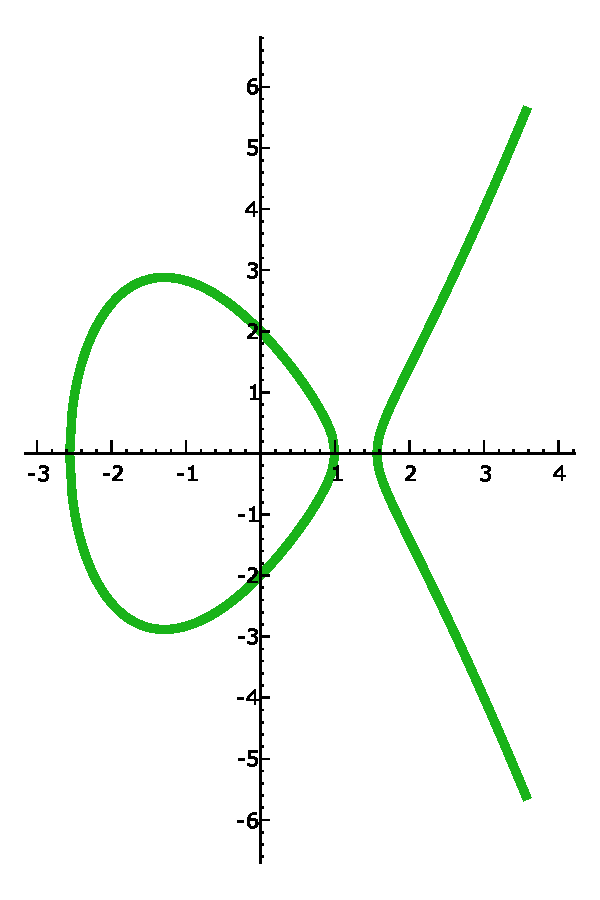
\includegraphics[width=0.4\textwidth]{graphics/eQ}
\caption{The elliptic curve $y^2  = x^3 - 5x + 4$ over $\R$\label{fig:ecQ}}
\end{center}
\end{figure}


We will use elliptic curves over finite fields to factor integers in
Section~\ref{sec:ecm} and to construct cryptosystems in
Section~\ref{sec:ec_crypto}.  The following Sage code creates an
elliptic curve over the finite field of order $37$ and plots it, as
illustrated in Figure~\ref{fig:ecf37}.
\newpage
\begin{verbatim}
sage: E = EllipticCurve(GF(37), [1,0])
sage: E
Elliptic Curve defined by y^2  = x^3 + x over
Finite Field of size 37
sage: E.plot(pointsize=45)
\end{verbatim}
\end{sg}

\begin{figure}[ht]
\begin{center}
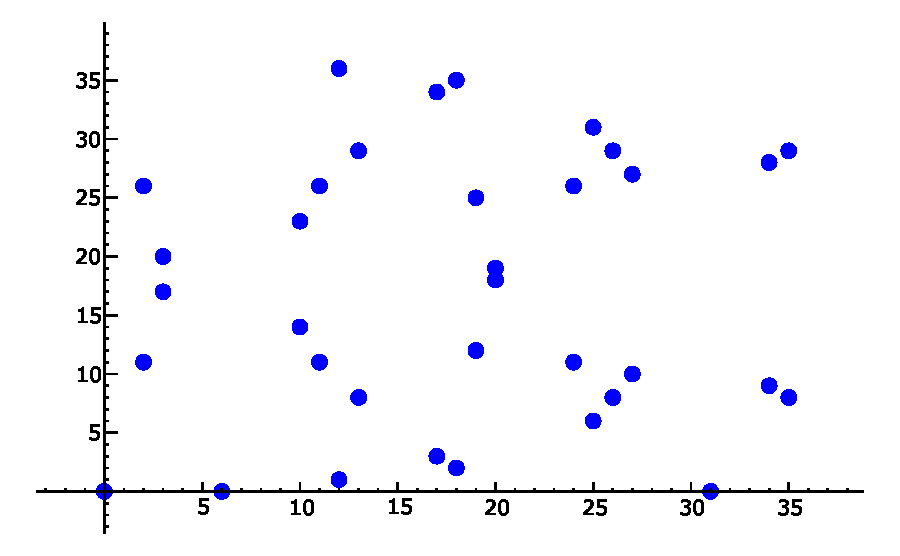
\includegraphics[width=0.6\textwidth]{graphics/E_gf37}
\caption{The elliptic curve $y^2 = x^3 + x$ over $\zmod{37}$\label{fig:ecf37}}
\end{center}
\end{figure}


In Section~\ref{sec:ellgrp}, we will put  a natural abelian
group structure on the set
$$
E(K) = \{ (x,y)\in K\cross K : y^2 = x^3 + ax +b \} \union \{\O\}
$$
of $K$-rational points on an elliptic curve~$E$ over~$K$.
Here,~$\O$ may be thought of as a point on~$E$ ``at infinity.''
Figure~\ref{fig:ecf37} contains a plot of the points
of $y^2=x^3+x$ over the finite field
$\zmod{37}$, though note that we do not explicitly draw the
point at $\O$ at infinity.

 %In Sections~\ref{sec:ecm}--\ref{sec:ec_crypto} we see how elliptic
% curves play a role in integer factorization algorithms, and how
% elliptic curves over finite fields provide cryptosystems that may in
% some ways to be much better than the cryptosystems from
% Chapter~\ref{ch:crypto}.
%In
% Section~\ref{sec:ellrat} we survey some results and conjectures about
% the groups $E(\Q)$ for elliptic curves $E$ over~$\Q$.

\begin{remark}
  If $K$ has characteristic $2$ (i.e., we have $1+1 = 0$ in $K$), then
  for any choice of $a,b$, the quantity $-16(4a^3+27b^2)\in K$ is $0$,
  so according to Definition~\ref{defn:ec} there are no elliptic
  curves over $K$.  There is a similar problem in characteristic $3$.
  If we instead consider equations of the form
$$
  y^2 + a_1 xy + a_3 y = x^3 + a_2 x^2 + a_4 x + a_6,
$$
we obtain a more general definition of elliptic curves, which
correctly allows for elliptic curves in characteristics $2$ and $3$;
these elliptic curves are popular in cryptography because arithmetic
on them is often easier to efficiently implement on a computer.
\end{remark}



\section{The Group Structure on an Elliptic Curve}\label{sec:ellgrp}\index{group!structure
of elliptic curve|nn}\index{elliptic curve!group structure|nn}


Let $E$ be an elliptic curve over a field  $K$,
given by an equation $y^2=x^3+ax+b$.
We begin by defining a binary operation $+$ on $E(K)$.
\begin{algorithm}{Elliptic Curve Group Law}\label{alg:grouplaw}
Given $P_1, P_2\in E(K)$,
this algorithm computes a third point $R=P_1+P_2 \in E(K)$.
\begin{steps}
\item{}[Is $P_i=\O$?] If $P_1=\O$ set $R=P_2$ or if $P_2=\O$ set $R=P_1$
and terminate.  Otherwise write $(x_i,y_i)=P_i$.
\item{}[Negatives]  If $x_1 = x_2$ and $y_1 = -y_2$, set $R=\O$ and terminate.
\item{}[Compute $\lambda$]\label{alg:grouplaw_3}
Set $\ds \lambda = \begin{cases}
 (3x_1^2+a)/(2y_1) & \text{if }P_1 = P_2,\\
(y_1-y_2)/(x_1-x_2) & \text{otherwise.}
\end{cases}$\\
\item{}[Compute Sum]\label{alg:grouplaw_4}  Then
$R = \ds \left(\lambda^2 -x_1 - x_2, -\lambda x_3 - \nu\right)$,
where $\nu = y_1 - \lambda x_1$ and  $x_3=\lambda^2 -x_1 - x_2$
is the $x$-coordinate of $R$.
\end{steps}
\end{algorithm}
Note that in Step~\ref{alg:grouplaw_3}, if $P_1=P_2$, then $y_1\neq 0$;
otherwise, we would have terminated in the previous step.

\begin{theorem}\label{thm:grouplaw}\ithm{elliptic curve group law}
  The binary operation $+$ defined in Algorithm~\ref{alg:grouplaw}
  endows the set $E(K)$ with an abelian group structure, with identity $\O$.
\end{theorem}

Before discussing why the theorem is true, we reinterpret $+$
geometrically, so that it will be easier for us to visualize.
We obtain the
sum $P_1+P_2$  by finding the third point $P_3$ of
intersection between~$E$ and the line~$L$ determined by $P_1$ and
$P_2$, then reflecting $P_3$ about the $x$-axis.
(This description requires suitable interpretation in
cases 1 and 2, and when $P_1=P_2$.) This is illustrated
in Figure~\ref{fig:geomgrouplaw}, in which $(0,2)+(1,0) = (3,4)$ on
$y^2=x^3-5x+4$.

\begin{sg}
We create the elliptic curve $y^2=x^3 - 5x + 4$ in Sage,
then add together $P=(1,0)$ and $Q=(0,2)$.   We also
compute $P + P$, which is the point $\mathcal{O}$ at infinity, which
is represented in Sage by $(0:1:0)$, and compute the sum
$P + Q + Q + Q + Q$, which is surprisingly large.
\begin{verbatim}
sage: E = EllipticCurve([-5,4])
sage: P = E([1,0]); Q = E([0,2])
sage: P + Q
(3 : 4 : 1)
sage: P + P
(0 : 1 : 0)
sage: P + Q + Q + Q + Q
(350497/351649 : 16920528/208527857 : 1)
\end{verbatim}
\end{sg}

To further clarify the above geometric interpretation of the group
law, we prove the following proposition.
\begin{proposition}[Geometric Group Law]\label{prop:geom_grouplaw}%
\iprop{geometric group law}
Suppose $P_i=(x_i,y_i)$, $i=1,2$ are distinct points on an elliptic
curve $y^2=x^3+ax+b$, and that $x_1\neq x_2$.  Let $L$ be
the unique line through $P_1$ and $P_2$.   Then $L$
intersects the graph of~$E$ at exactly one other point
$$
  Q = \left(\lambda^2 -x_1 - x_2,\quad \lambda x_3 + \nu\right),
$$
where $\lambda = (y_1-y_2)/(x_1-x_2)$ and $\nu = y_1 - \lambda x_1$.
\end{proposition}
\begin{proof}
  The line $L$ through $P_1$, $P_2$ is $y = y_1 + (x-x_1)\lambda$.
  Substituting this into $y^2=x^3+ax+b$, we get
  $$
  (y_1+(x-x_1)\lambda)^2 = x^3 + ax + b.
  $$
  Simplifying, we get $f(x) = x^3 - \lambda^2 x^2 + \cdots = 0$, where we
  omit the coefficients of $x$ and the constant term since they will
not be needed.
  Since $P_1$ and $P_2$ are in $L\cap E$, the polynomial $f$
  has $x_1$ and $x_2$ as roots.  By Proposition~\ref{prop:atmost},
the polynomial~$f$
  can have at most three roots.   Writing $f=\prod(x-x_i)$
and equating terms, we see that
 $x_1+x_2 + x_3 = \lambda^2$.  Thus, $x_3 = \lambda^2 - x_1-x_2$,
as claimed.  Also, from the equation for~$L$ we see that
$y_3 = y_1 + (x_3 - x_1)\lambda = \lambda x_3 + \nu$, which
completes the proof.
\end{proof}

\begin{figure}
\begin{center}\index{group law!illustrated}\index{graph!of group law}
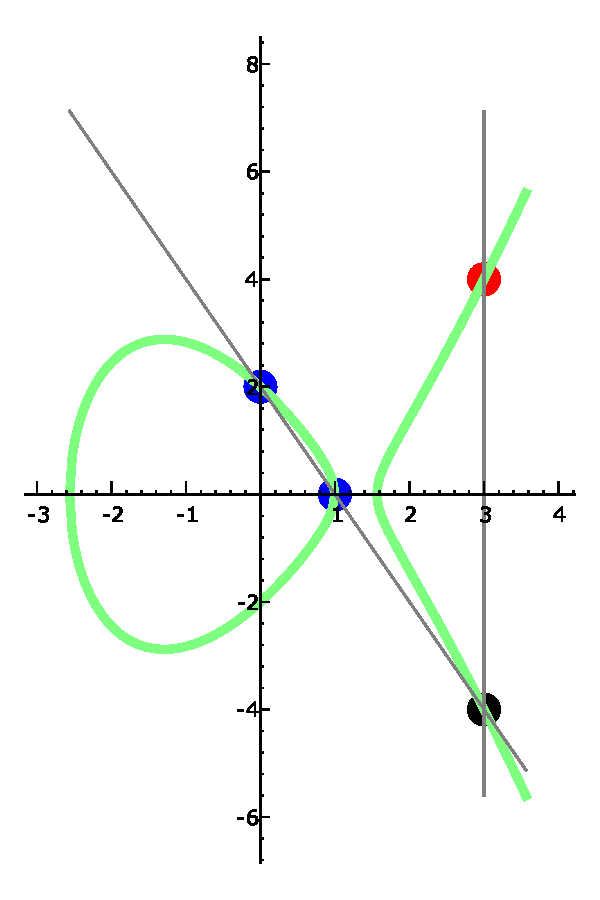
\includegraphics[width=0.4\textwidth]{graphics/gplaw}
\caption{The Group Law: $(1,0)+(0,2)=(3,4)$ on $y^2=x^3-5x+4$}
\label{fig:geomgrouplaw}
\end{center}
\end{figure}

To prove Theorem~\ref{thm:grouplaw} means to show that $+$ satisfies
the three axioms of an abelian group with $\O$ as identity element:
existence of inverses, commutativity, and associativity.  The
existence of inverses follows immediately from the definition, since
$(x,y)+(x,-y)=\O$.  Commutativity is also clear from the definition of
group law, since in Parts 1--3, the recipe is unchanged if we
swap~$P_1$ and~$P_2$; in Part 4 swapping~$P_1$ and~$P_2$ does not
change the line determined by~$P_1$ and~$P_2$, so by
Proposition~\ref{prop:geom_grouplaw} it does not change the sum
$P_1+P_2$.

It is more difficult to prove that $+$ satisfies the associative
axiom, i.e., that $(P_1+P_2)+P_3 = P_1 + (P_2 + P_3)$.  This fact can
be understood from at least three points of view.  One is to
reinterpret the group law geometrically (extending
Proposition~\ref{prop:geom_grouplaw} to all cases), and thus transfer
the problem to a question in plane geometry.  This approach is
beautifully explained with exactly the right level of detail in
\cite[\S I.2]{silvermantate}. Another approach is to use the formulas
that define $+$ to reduce associativity to checking specific algebraic
identities; this is something that would be extremely tedious to do by
hand, but can be done using a computer (also tedious).
%We give part of such a computer proof
%in Section~\ref{sec:grouplawproof} below.
A third approach (see \cite{silverman:aec} or
\cite{hartshorne}) is to develop a general theory of ``divisors on
algebraic curves,'' from which associativity of the group law falls
out as a natural corollary.  The third approach is the best, because
it opens up many new vistas; however, we will not pursue it further
because it is beyond the scope of this book.

\begin{sg}
  In the following Sage session, we use the formula from
  Algorithm~\ref{alg:grouplaw} to verify that the group law holds for
  any choice of points $P_1, P_2, P_3$ on any elliptic curve over $\Q$
  such that the points $P_1, P_2, P_3, P_1+P_2, P_2+P_3$ are all
  distinct and nonzero.  We define a polynomial ring $R$ in 8
  variables.
\begin{verbatim}
sage: R.<x1,y1,x2,y2,x3,y3,a,b> = QQ[]
\end{verbatim}%link
\vspace{1ex}

\noindent{}We define the relations the $x_i$ will satisfy, and a
quotient ring $Q$ in which those relations are satisfied.  (Quotients
of polynomial rings are a generalization of the construction $\Z/n\Z$
that may be viewed as the quotient of the ring $\Z$ of integers by the
relation that sets $n$ to equal $0$.)
%link
\begin{verbatim}
sage: rels = [y1^2 - (x1^3 + a*x1 + b),
...           y2^2 - (x2^3 + a*x2 + b),
...           y3^2 - (x3^3 + a*x3 + b)]
...
sage: Q = R.quotient(rels)
\end{verbatim}%link
\vspace{1ex}

\noindent{}We define the group operation, which assumes the points are distinct.
%link
\begin{verbatim}
sage: def op(P1,P2):
...       x1,y1 = P1;  x2,y2 = P2
...       lam = (y1 - y2)/(x1 - x2); nu  = y1 - lam*x1
...       x3 = lam^2 - x1 - x2; y3 = -lam*x3 - nu
...       return (x3, y3)
\end{verbatim}%link
\vspace{1ex}

\noindent{}We define three points, add them together via $P_1 + (P_2 + P_3)$
and $(P_1 + (P_2 + P_3))$, and observe that the results are the same modulo the relations.
%link
\begin{verbatim}
sage: P1 = (x1,y1); P2 = (x2,y2); P3 = (x3,y3)
sage: Z = op(P1, op(P2,P3)); W = op(op(P1,P2),P3)
sage: (Q(Z[0].numerator()*W[0].denominator() -
...          Z[0].denominator()*W[0].numerator())) == 0
True
sage: (Q(Z[1].numerator()*W[1].denominator() -
...          Z[1].denominator()*W[1].numerator())) == 0
True
\end{verbatim}
\end{sg}


\section{Integer Factorization Using Elliptic Curves}\index{factorization!using elliptic curves}
\index{elliptic curve!factorization}
\label{sec:ecm}
In 1987, Hendrik Lenstra\index{Lenstra|(}\index{ECM|(}
published the landmark paper
\cite{lenstra:factorell} that introduces and analyzes
the Elliptic Curve Method (ECM)\index{ECM}, which is
a powerful algorithm for factoring integers
using elliptic curves.  Lenstra's method is also described in
\cite[\S IV.4]{silvermantate},
\cite[\S VIII.5]{davenport},  and
\cite[\S 10.3]{cohen:ant}.

\vspace{3ex}
\noindent\begin{minipage}[b]{.67\linewidth}
  Lenstra's algorithm is well suited for finding ``medium-sized''
  factors of an integer~$N$, which today means between~$10$ to~$40$ decimal
  digits.  The ECM method is not {\em directly} used for factoring
  RSA challenge numbers (see Section~\ref{sec:numfact}), but it is
  used on auxiliary numbers as a crucial step in the ``number field
  sieve,'' which is the best known algorithm for hunting for such
  factorizations.  Also, implementation of ECM typically requires little
  memory.
\end{minipage}\hspace{.05\linewidth}
\begin{minipage}[b]{.25\linewidth}
\noindent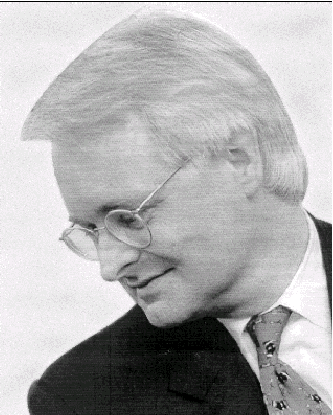
\includegraphics[width=\textwidth]{graphics/lenstra}
\vspace{-3ex}
\begin{center}
H. Lenstra
\end{center}
\end{minipage}
\vspace{-2ex}


\subsection{Pollard's $(p-1)$-Method}\label{sec:pollard}
\index{Pollard's $(p-1)$-method|(}\index{factorization!Pollard's $(p-1)$-method|(}
Lenstra's discovery of ECM was inspired by
Pollard's $(p-1)$-method, which we describe in this section.
\begin{definition}[Power Smooth]%
  \index{power smooth|nn}\index{smooth|nn} Let~$B$ be a positive
  integer. If~$n$ is a positive integer with prime factorization
  $n=\prod p_i^{e_i}$, then $n$ is \defn{$B$-power smooth} if
  $p_i^{e_i}\leq B$ for all $i$.
\end{definition}
For example, $30=2\cdot 3\cdot 5$ is $B$ power smooth for $B=5, 7$, but
$150=2\cdot 3 \cdot 5^2$ is not $5$-power smooth (it is $B=25$-power
smooth).

We will use the following algorithm in both the Pollard $p-1$
and elliptic curve factorization methods.
\begin{algorithm}{Least Common Multiple of First $B$ Integers}
\label{alg:lcmupto}
Given a positive integer $B$, this algorithm computes the least
common multiple of the positive integers up to $B$.
\begin{steps}
\item{}[Sieve] Using, for example, the prime sieve
  (Algorithm~\ref{alg:sieve}), compute a list~$P$ of all primes $p\leq
  B$.
\item{}[Multiply]
Compute and output the product $\prod_{p\in P} p^{\lfloor \log_p(B) \rfloor}$.
\end{steps}
\end{algorithm}
\begin{proof}
Set $m=\lcm(1,2,\ldots, B)$.  Then,
$$
  \ord_p(m) = \max(\{\ord_p(n) : 1 \leq n \leq B\}) = \ord_p(p^r),
$$
where $p^r$ is the largest power of $p$ that satisfies $p^r\leq B$.
Since $p^r\leq B < p^{r+1}$, we have $r=\lfloor \log_p(B) \rfloor$.
\end{proof}

\begin{sg}
  We implement Algorithm~\ref{alg:lcmupto} in Sage and compute the
  least common multiple for $B=100$ using both the above algorithm and
  a naive algorithm.  We use {\tt math.log} below so that $\log_p(B)$
  is computed quickly using double precision numbers.
\begin{verbatim}
sage: def lcm_upto(B):
...       return prod([p^int(math.log(B)/math.log(p))
...                    for p in prime_range(B+1)])
sage: lcm_upto(10^2)
69720375229712477164533808935312303556800
sage: LCM([1..10^2])
69720375229712477164533808935312303556800
\end{verbatim}
Algorithm~\ref{alg:lcmupto} as implemented above in Sage takes about a
second for $B=10^6$.
\end{sg}

Let~$N$ be a positive integer that we wish to factor.  We use the
Pollard $(p-1)$-method to look for a nontrivial factor of~$N$ as
follows.  First, we choose a positive integer~$B$, usually with at
most six digits.  Suppose that there is a prime divisor~$p$ of~$N$
such that $p-1$ is $B$-power smooth.  We try to find~$p$ using the
following strategy.  If $a>1$ is an integer not divisible by~$p$, then
by Theorem~\ref{thm:fermatlittle},
$$a^{p-1}\con 1\pmod{p}.$$
Let $m=\lcm(1,2,3,\ldots, B)$, and observe that our assumption that
$p-1$ is $B$-power smooth implies that $p-1\mid m$, so
$$
  a^m \con 1 \pmod{p}.
$$
Thus
$$
  p\mid \gcd(a^m-1,N) > 1.
$$
If $\gcd(a^m-1,N)<N$ also then $\gcd(a^m-1,N)$ is a nontrivial factor
of~$N$.
If $\gcd(a^m-1,N)=N$, then $a^m\con 1\pmod{q^r}$ for every prime power
divisor $q^r$ of~$N$.  In this case, repeat the above steps but with a
smaller choice of~$B$ or possibly a different choice of~$a$.
Also, it is a good idea to check from the
start whether or not~$N$ is not a perfect power $M^r$ and, if so,
replace~$N$ by~$M$. We formalize the algorithm as follows:

\begin{algorithm}{Pollard $p-1$ Method}\label{alg:pollard}
  Given a positive integer $N$ and a bound $B$, this algorithm
  attempts to find a nontrivial factor $g$ of $N$.  (Each prime $p\mid
  g$ is likely to have the property that $p-1$ is $B$-power smooth.)
\begin{steps}
\item{}[Compute lcm]
Use Algorithm~\ref{alg:lcmupto} to compute $m=\lcm(1,2,\ldots, B)$.
\item{}[Initialize] Set $a\assign 2$.
\item{}[Power and gcd]\label{alg:pollard_3}
Compute $x \assign a^m - 1\pmod{N}$
and $g=\gcd(x,N)$.
\item{}[Finished?]
If $g\neq 1$ or $N$, output $g$ and terminate.
\item{}[Try Again?] If $a<10$ (say), replace $a$ by $a+1$ and go to step
  \ref{alg:pollard_3}.  Otherwise, terminate.
\end{steps}
\end{algorithm}


For fixed~$B$, Algorithm~\ref{alg:pollard} often splits~$N$ when~$N$
is divisible by a prime~$p$ such that $p-1$ is $B$-power smooth.
Approximately 15 percent of primes~$p$ in the interval from $10^{15}$
and $10^{15}+10000$ are such that $p-1$ is $10^6$ power smooth, so the
Pollard method with $B=10^6$ already fails nearly 85 percent of the
time at finding~$15$-digit primes in this range (see also
\exref{ch:ec}{ex:bpowersmooth}).  We will not analyze Pollard's method
further, since it was mentioned here only to set the stage for the
elliptic curve factorization method.

The following examples illustrate the Pollard $(p-1)$-method.
\begin{example}
In this example, Pollard works perfectly.
Let $N=5917$.  We try to use the Pollard $p-1$ method with
$B=5$ to split~$N$.  We have
$m = \lcm(1,2,3,4,5)=60$; taking $a=2$, we have
$$
  2^{60} - 1 \con 3416\pmod{5917}
$$
and
$$
 \gcd(2^{60}-1,5917) = \gcd(3416,5917) = 61,
$$
so $61$ is a factor of~$5917$.
\end{example}

\begin{example}
In this example, we replace~$B$ with a larger integer.
Let $N=779167$.  With $B=5$ and $a=2$, we have
$$
   2^{60}-1 \con 710980\pmod{779167},
$$
and $\gcd(2^{60}-1,779167) = 1.$
With $B=15$, we have $$m=\lcm(1,2,\ldots,15)=360360,$$
$$
  2^{360360}-1 \con 584876\pmod{779167},
$$
and
$$\gcd(2^{360360}-1 , N) = 2003,$$
so $2003$ is a nontrivial factor of~$779167$.
\end{example}


\begin{example}
In this example, we replace~$B$ by a smaller integer.
Let $N=4331$. Suppose  $B=7$, so $m=\lcm(1,2,\ldots,7)=420$,
$$
  2^{420} - 1 \con 0 \pmod{4331},
$$
and $\gcd(2^{420} - 1, 4331) = 4331$,
so we do not obtain a factor of~$4331$.
If we replace~$B$ by $5$, Pollard's method works:
$$
  2^{60} - 1\con 1464\pmod{4331},
$$
and $\gcd(2^{60}-1,4331) = 61$,
so we split~$4331$.
\end{example}

\begin{example}
In this example, $a=2$ does not work, but $a=3$ does.
Let $N=187$. Suppose  $B=15$, so $m=\lcm(1,2,\ldots,15)=360360$,
$$
  2^{360360} - 1 \con 0 \pmod{187},
$$
and $\gcd(2^{360360} - 1, 187) = 187$,
so we do not obtain a factor of~$187$.
If we replace $a=2$ by $a=3$, then Pollard's method works:
$$
  3^{360360} - 1\con 66\pmod{187},
$$
and $\gcd(3^{360360}-1,187) = 11$.  Thus $187 = 11\cdot 17$.
\end{example}
\index{Pollard's $(p-1)$-method|)}\index{factorization!Pollard's $(p-1)$-method|)}
\begin{sg}
We implement the Pollard $(p-1)$-method in Sage and use our implementation
to do all of the above examples.
\begin{verbatim}
sage: def pollard(N, B=10^5, stop=10):
...       m = prod([p^int(math.log(B)/math.log(p))
...                 for p in prime_range(B+1)])
...       for a in [2..stop]:
...           x = (Mod(a,N)^m - 1).lift()
...           if x == 0: continue
...           g = gcd(x, N)
...           if g != 1 or g != N: return g
...       return 1
sage: pollard(5917,5)
61
sage: pollard(779167,5)
1
sage: pollard(779167,15)
2003
sage: pollard(4331,7)
1
sage: pollard(4331,5)
61
sage: pollard(187, 15, 2)
1
sage: pollard(187, 15)
11
\end{verbatim}
\end{sg}

\subsection{Motivation for the Elliptic Curve Method}
Fix a positive integer~$B$.  If $N=pq$ with $p$ and $q$ prime, and we
assume that $p-1$ and $q-1$ are not $B$-power smooth, then the Pollard
$(p-1)$-method is unlikely to work.  For example, let $B=20$ and
suppose that $N=59\cdot 101 = 5959$.  Note that
neither~$59-1=2\cdot29$ nor $101-1=4\cdot 25$ is $B$-power smooth.
With $m=\lcm(1,2,3,\ldots,20)=232792560$, we have
$$2^m - 1 \con 5944\pmod{N},$$
and $\gcd(2^m-1,N)=1$, so we do not find a factor of~$N$.

As remarked above, the problem is that $p-1$ is not $20$-power smooth for
either $p=59$ or $p=101$.  However, notice that $p-2=3\cdot 19$ is
$20$-power smooth.  Lenstra's\index{Lenstra|)} ECM  replaces
$(\zmod{p})^*$, which has order $p-1$, by the group of points
on an elliptic curve~$E$ over $\zmod{p}$.
It is a theorem that
$$
 \#E(\zmod{p}) =p+1\pm s
$$
for some nonnegative integer $s<2\sqrt{p}$
(see \cite[\S V.1]{silverman:aec} for a proof).
Also, every value of~$s$ subject to this
bound occurs, as one can see using ``complex multiplication
theory.''
For example, if~$E$ is the elliptic curve
\[
   y^2 = x^3 + x + 54
\]
over $\zmod{59}$, then by enumerating points one sees that
$E(\zmod{59})$ is cyclic of order~$57$.  The set of numbers $59+1\pm
s$ for $s\leq 15$ contains~$14$ numbers that are $B$-power smooth
for~$B=20$, which illustrates that working with an elliptic curve
gives us more flexibility.  For example, $60=59+1+0$ is $5$-power
smooth and $70 = 59+1+10$ is $7$-power smooth.


\subsection{Lenstra's Elliptic Curve Factorization Method}\label{sec:ecm_describe}
\index{elliptic curve!factorization|nn}

%\begin{figure}
%\begin{center}
%\includegraphics[width=0.8in]{graphics/lenstra_ober}
%\end{center}
%\caption{Hendrik Lenstra}
%\end{figure}

\begin{algorithm}{Elliptic Curve Factorization Method}\label{alg:ecm}
Given a positive integer~$N$ and a bound~$B$, this algorithm
attempts to find a nontrivial factor~$g$ of~$N$ or outputs
``Fail.''
\begin{steps}
\item{}[Compute lcm]
Use Algorithm~\ref{alg:lcmupto} to compute $m=\lcm(1,2,\ldots, B)$.
\item{}[Choose Random Elliptic Curve]
Choose a random $a\in \zmod{N}$ such that $4a^3+27\in(\zmod{N})^*$.
Then $P=(0,1)$ is a point on the elliptic curve $y^2=x^3+ax+1$
over $\zmod{N}$.
\item{}[Compute Multiple] Attempt to compute $m P$ using an
elliptic curve analog of Algorithm~\ref{alg:power}.
If at some point we cannot compute a sum of points
because some denominator in Step~\ref{alg:grouplaw_3} of
Algorithm~\ref{alg:grouplaw} is not coprime to~$N$, we
compute the greatest common divisor $g$ of this denominator with~$N$.  If $g$
is a nontrivial divisor, output it.  If every
denominator is coprime to~$N$, output ``Fail.''
\end{steps}
\end{algorithm}

If Algorithm~\ref{alg:ecm} fails for one random elliptic curve, there
is an option that is unavailable with Pollard's $(p-1)$-method---we
may repeat the above algorithm with a different elliptic curve.  With
Pollard's method we always work with the group $(\zmod{N})^*$, but
here we can try many groups $E(\zmod{N})$ for many curves $E$.  As
mentioned above, the number of points on~$E$ over $\zmod{p}$ is of the
form $p+1-t$ for some~$t$ with $|t|<2\sqrt{p}$;
Algorithm~\ref{alg:ecm} thus has a chance if $p+1-t$ is
$B$-power smooth for some $t$ with $|t|<2\sqrt{p}$.

\subsection{Examples}\label{sec:ecm_examples}
For simplicity, we use an elliptic curve of the form
$$y^2 = x^3 + ax + 1,$$
which has the point $P=(0,1)$ already on it.

We factor $N=5959$ using the elliptic curve method.
Let
$$
  m=\lcm(1,2,\ldots,20) = 232792560 = 1101111000000010000111110000_2,
$$
where $x_2$ means~$x$ is written in binary.
First, we choose $a=1201$ at random and consider
$y^2 = x^3 + 1201x + 1$ over $\zmod{5959}$.
%% \conrad{Aarg, maybe not
%% a field, so why can we make sense of elliptic curve, group law,
%% etc.?}
Using the formula for $P+P$ from
Algorithm~\ref{alg:grouplaw}
we compute
$2^i\cdot P = 2^i\cdot (0,1)$
for $i\in B=\{4, 5, 6, 7, 8, 13, 21, 22, 23, 24, 26, 27 \}$.
Then $\sum_{i\in B} 2^i P = m P$.  It turns out that during no
step of this computation does a number not coprime to
$5959$ appear in any denominator, so we do not split~$N$
using $a=1201$.  Next, we try $a=389$ and at some stage
in the computation we add
$P=(2051,5273)$ and $Q=(637,1292)$.
When computing the group law explicitly, we try
to compute $\lambda = (y_1-y_2)/(x_1-x_2)$ in $(\Z/5959\Z)^*$,
but we fail since $x_1-x_2 = 1414$ and $\gcd(1414,5959)=101$.
We thus find a nontrivial factor $101$ of $5959$.

\begin{sg}
  We implement elliptic curve factorization in Sage, then
  use it to do the above example and some other examples.
\begin{verbatim}
sage: def ecm(N, B=10^3, trials=10):
...       m = prod([p^int(math.log(B)/math.log(p))
...                 for p in prime_range(B+1)])
...       R = Integers(N)
...       # Make Sage think that R is a field:
...       R.is_field = lambda : True
...       for _ in range(trials):
...           while True:
...               a = R.random_element()
...               if gcd(4*a.lift()^3 + 27, N) == 1: break
...           try:
...               m * EllipticCurve([a, 1])([0,1])
...           except ZeroDivisionError, msg:
...               # msg: "Inverse of <int> does not exist"
...               return gcd(Integer(str(msg).split()[2]), N)
...       return 1
sage: set_random_seed(2)
sage: ecm(5959, B=20)
101
sage: ecm(next_prime(10^20)*next_prime(10^7), B=10^3)
10000019
\end{verbatim}
\end{sg}

\subsection{A Heuristic Explanation}\label{sec:methods}
Let $N$ be a positive integer and, for simplicity of exposition,
assume that $N=p_1\cdots p_r$ with the $p_i$ distinct primes.
It follows from Lemma~\ref{lem:units_map} that there is a
natural isomorphism
$$
f : (\Z/N\Z)^* \lra (\Z/p_1\Z)^* \cross \cdots \cross (\Z/p_r\Z)^*.
$$
When using Pollard's method, we choose an $a\in (\Z/N\Z)^*$,
compute $a^m$, then compute $\gcd(a^m-1,N)$.  This $\gcd$ is divisible
exactly by the primes~$p_i$ such that $a^m \con 1\pmod{p_i}$.  To
reinterpret Pollard's method using the above isomorphism, let
$(a_1,\ldots,a_r) = f(a)$.  Then $(a_1^m,\ldots,a_r^m) = f(a^m)$, and
the $p_i$ that divide $\gcd(a^m-1,N)$ are exactly the $p_i$ such that
$a_i^m=1$.  By Theorem~\ref{thm:fermatlittle}, these $p_i$ include the
primes~$p_j$ such that $p_j-1$ is $B$-power smooth, where
$m=\lcm(1,\ldots,m)$.

We will not define $E(\zmod{N})$ when~$N$ is composite, since this is
not needed for the algorithm (where we assume that~$N$ is prime and
hope for a contradiction).  However, for the remainder of this
paragraph, we pretend that $E(\zmod{N})$ is meaningful and describe a
heuristic connection between Lenstra and Pollard's methods.  The
significant difference between Pollard's method and the elliptic curve
method is that the isomorphism~$f$ is replaced by an isomorphism (in
quotes)
$$
``g : E(\zmod{N}) \ra E(\zmod{p_1}) \cross \cdots \cross E(\zmod{p_r}) \mbox{\rm ''}
$$
where $E$ is $y^2=x^3+ax+1$, and the~$a$ of Pollard's method is
replaced by $P=(0,1)$.  We put the isomorphism in quotes to emphasize
that we have not defined $E(\zmod{N})$.  When carrying out the
elliptic curve factorization algorithm, we attempt to compute $mP$,
and if some components of $f(Q)$ are $\O$, for some point~$Q$ that
appears during the computation, but others are nonzero, we find a
nontrivial factor of~$N$.


%%%%%%%%%%%%%%%%%%%%%%%%%%%%%%%%%%%%%%%%%%%%%%%%%%%%%%
\section{Elliptic Curve Cryptography}\index{elliptic curve!cryptography}
\index{cryptography!using elliptic curves}\label{sec:ec_crypto}

The idea to use elliptic curves in cryptography was independently
proposed by Neil Koblitz and Victor Miller in the mid 1980s.  In this
section, we discuss an analog of Diffie-Hellman that uses an
elliptic curve instead of $(\zmod{p})^*$.  We then discuss the ElGamal
elliptic curve cryptosystem.

\subsection{Elliptic Curve Analogs of Diffie-Hellman}
\label{sec:ec_crypto_analogues}
The Diffie-Hellman\index{Diffie-Hellman cryptosystem!on elliptic curve}
\index{elliptic curve!Diffie-Hellman}
key exchange from Section~\ref{sec:diffie}
works well on an elliptic curve
with no serious modification.
Michael\index{Michael} and Nikita\index{Nikita}
agree on a secret key as follows:
\begin{enumerate}
\item Michael and Nikita agree on a prime~$p$, an
elliptic curve~$E$ over $\zmod{p}$, and a point $P\in E(\zmod{p})$.
\item Michael secretly chooses a random~$m$ and sends $mP$.
\item Nikita secretly chooses a random~$n$ and sends $nP$.
\item The secret key is $nmP$, which both Michael and
Nikita can compute.
\end{enumerate}
Presumably, an adversary can not compute $nmP$ without solving the
discrete logarithm problem\index{discrete log problem!on elliptic
  curve} \index{elliptic curve!discrete log problem} (see
Problem~\ref{prob:log} and Section~\ref{sec:ecdl} below) in
$E(\zmod{p})$.  For well-chosen $E$, $P$, and~$p$, experience suggests
that the discrete logarithm problem in $E(\zmod{p})$ is much more
difficult than the discrete logarithm problem in $(\zmod{p})^*$ (see
Section~\ref{sec:ecdl} for more on the elliptic curve discrete log
problem).


\subsection{The ElGamal Cryptosystem and
  Digital Rights Management}\label{sec:elgamal}
This section is about
the ElGamal cryptosystem\index{cryptosystem!ElGamal}, \index{ElGamal
  cryptosystem} which works well on an elliptic curve.  This section
draws on a paper by a computer hacker named Beale Screamer who
cracked a ``Digital Rights Management'' (DRM) system.

The elliptic curve used in the DRM is an elliptic curve over the
finite field $k=\zmod{p}$, where
$$
  p=785963102379428822376694789446897396207498568951.
$$
The number $p$ in base 16 is
\begin{center}
89ABCDEF012345672718281831415926141424F7,
\end{center}
which includes counting in hexadecimal, and digits of~$e$,
$\pi$, and $\sqrt{2}$.
The elliptic curve~$E$ is
\begin{align*}
y^2 = x^3 &+ 317689081251325503476317476413827693272746955927x \\
             &\qquad +79052896607878758718120572025718535432100651934.
\end{align*}
We have
$$\# E(k) = 785963102379428822376693024881714957612686157429,$$
and the group $E(k)$ is cyclic with generator
\begin{align*}
B &= (771507216262649826170648268565579889907769254176, \\
&\qquad 390157510246556628525279459266514995562533196655).
\end{align*}

Our heroes Nikita\index{Nikita} and Michael\index{Michael} share
digital music when they are not out fighting terrorists.  When Nikita
installed the DRM software on her computer, it generated a private key
$$
n = 670805031139910513517527207693060456300217054473,
$$
which it hides in bits and pieces of files.  In order for Nikita to
play Juno Reactor's latest hit {\tt juno.wma}, her web browser contacts a
website that sells music.  After Nikita sends her credit card number,
that website allows Nikita to download a license file that allows
her audio player to unlock and play {\tt juno.wma}.

As we will see below, the license file was created using the ElGamal
public-key cryptosystem\index{ElGamal
  cryptosystem}\index{cryptosystem!ElGamal} in the group $E(k)$.
Nikita can now use her license file to unlock {\tt juno.wma}.
However, when she shares both {\tt juno.wma} and the license file with
Michael, he is frustrated because even with the license, his computer
still does not play {\tt juno.wma}.  This is because Michael's computer
does not know Nikita's computer's private key (the integer~$n$ above),
so Michael's computer can not decrypt the license file.
%\begin{center}
%\includegraphics[width=1.9in]{graphics/juno}\\
%\end{center}

\index{cryptosystem!ElGamal}
We now describe the ElGamal cryptosystem, which lends itself well to
implementation in the group $E(\zmod{p})$.  To illustrate ElGamal, we
describe how Nikita would set up an ElGamal cryptosystem that anyone
could use to encrypt messages for her.  Nikita chooses a prime~$p$, an
elliptic curve~$E$ over $\zmod{p}$, and a point $B\in E(\zmod{p})$, and
publishes~$p$,~$E$, and~$B$.  She also chooses a random integer~$n$,
which she keeps secret, and publishes $nB$.  Her public key is the
four-tuple $(p,E,B, nB)$.

Suppose Michael wishes to encrypt a message for Nikita.
If the message is encoded as an element $P\in E(\zmod{p})$,
Michael computes a random integer~$r$ and the
points $rB$ and $P+r(nB)$ on $E(\zmod{p})$.
Then~$P$ is encrypted as the pair
$(rB, P+r(nB))$. To decrypt the encrypted message,
Nikita multiplies $rB$ by her secret key~$n$
to find $n(rB) = r(nB)$, then subtracts this from
$P+r(nB)$ to obtain
  $$P = P+r(nB)-r(nB).$$
%We implement this cryptosystem in Section~\ref{sec:comp_elgamal}.

\begin{remark}
  It also make sense to construct an ElGamal cryptosystem in the group
  $(\zmod{p})^*$.
\end{remark}

Returning to our story, Nikita's license file is an encrypted message
to her.  It contains the pair of points $(rB,P+r(nB))$, where
\begin{align*}
  rB &= (179671003218315746385026655733086044982194424660,\\
    & \qquad\quad  697834385359686368249301282675141830935176314718)
\end{align*}
and
\begin{align*}
  P+r(nB) &= (137851038548264467372645158093004000343639118915,\\
&\qquad\quad 110848589228676224057229230223580815024224875699).
\end{align*}
When Nikita's computer plays {\tt juno.wma}, it loads the secret key
$$
n = 670805031139910513517527207693060456300217054473
$$
into memory and computes
\begin{align*}
n(rB) &=
  (328901393518732637577115650601768681044040715701,\\
   & \qquad 586947838087815993601350565488788846203887988162).
\end{align*}
It then subtracts this from $P+r(nB)$ to obtain
\begin{align*}
  P &= (14489646124220757767, \\
    &  \quad\qquad 669337780373284096274895136618194604469696830074).
\end{align*}

\noindent{}The $x$-coordinate $14489646124220757767$ is the
key that unlocks {\tt juno.wma}.


If Nikita knew the private key~$n$ that her computer generated, she
could compute~$P$ herself and unlock {\tt juno.wma} and share her
music with Michael.  Beale Screamer found a weakness in the
implementation of this system that allows Nikita to detetermine~$n$,
which is not a huge surprise since~$n$ is stored on her computer after
all.

\begin{sg}
We do the above examples in Sage:
\begin{verbatim}
sage: p = 785963102379428822376694789446897396207498568951
sage: E = EllipticCurve(GF(p), \
...    [317689081251325503476317476413827693272746955927,
...     79052896607878758718120572025718535432100651934])
sage: E.cardinality()
785963102379428822376693024881714957612686157429
sage: E.cardinality().is_prime()
True
sage: B = E([
...    771507216262649826170648268565579889907769254176,
...    390157510246556628525279459266514995562533196655])
sage: n=670805031139910513517527207693060456300217054473
sage: r=70674630913457179596452846564371866229568459543
sage: P = E([14489646124220757767,
...    669337780373284096274895136618194604469696830074])
sage: encrypt = (r*B, P + r*(n*B))
sage: encrypt[1] - n*encrypt[0] == P   # decrypting works
True
\end{verbatim}
\end{sg}

\subsection{The Elliptic Curve Discrete Logarithm Problem}\label{sec:ecdl}
\index{elliptic curve!discrete log problem}
\index{discrete log problem!on elliptic curve}
\begin{problem}[Elliptic Curve Discrete Log Problem]
  Suppose~$E$ is an elliptic curve over $\zmod{p}$ and~$P\in
  E(\zmod{p})$.  Given a multiple~$Q$ of~$P$, the \defn{elliptic curve
    discrete log problem} is to find $n\in\Z$ such that $nP=Q$.
\end{problem}

For example, let $E$ be the elliptic curve given by $y^2 = x^3 + x+1$
over the field $\zmod{7}$.  We have
$$
  E(\zmod{7}) = \{\O, (2, 2), (0,1), (0,6), (2,5) \}.
$$
If $P=(2,2)$ and $Q=(0,6)$, then $3P=Q$, so $n=3$
is a solution to the discrete logarithm problem.

If $E(\zmod{p})$ has order $p$ or $p\pm 1$, or is a product of
reasonably small primes, then there are some methods for attacking the
discrete log problem on~$E$, which are beyond the scope of this book.
It is therefore important to be able to compute $\#E(\zmod{p})$
efficiently, in order to verify that the elliptic curve one wishes to
use for a cryptosystem doesn't have any obvious vulnerabilities.  The
naive algorithm to compute $\#E(\zmod{p})$ is to try each value of
$x\in\zmod{p}$ and count how often $x^3+ax+b$ is a perfect square
mod~$p$, but this is of no use when $p$ is large enough to be useful
for cryptography.  Fortunately, there is an algorithm due to Schoof,
Elkies, and Atkin for computing $\#E(\zmod{p})$ efficiently
(polynomial time in the number of digits of $p$), but this algorithm
is beyond the scope of this book.
%% TODO: Give reference for this algorithm.

In Section~\ref{sec:dlog}, we discussed the discrete log problem in
$(\zmod{p})^*$.  There are general attacks called ``index calculus
attacks'' on the discrete log problem in $(\zmod{p})^*$ that are slow,
but still faster than the known algorithms for solving the discrete
log in a ``general'' group (one with no extra structure).  For most
elliptic curves, there is no known analog of index calculus attacks
on the discrete log problem.  At present, it appears that given~$p$,
the discrete log problem in $E(\zmod{p})$ is much harder than the
discrete log problem in the multiplicative group $(\zmod{p})^*$.  This
suggests that by using an elliptic curve-based cryptosystem instead of
one based on $(\zmod{p})^*$, one gets equivalent security with much
smaller numbers, which is one reason why building cryptosystems using
elliptic curves is attractive to some cryptographers.  For example,
Certicom, a company that strongly supports elliptic curve
cryptography, claims:
\begin{quote}
``[Elliptic curve crypto] devices require less storage, less
power, less memory, and less bandwidth than other systems. This allows
you to implement cryptography in platforms that are constrained, such
as wireless devices, handheld computers, smart cards, and
thin-clients. It also provides a big win in situations where
efficiency is important.''
\end{quote}

For an up-to-date list of elliptic curve discrete log challenge
problems that Certicom sponsors, see \cite{certicom:challenge}.  For
example, in April 2004, a specific cryptosystem was cracked that was
based on an elliptic curve over $\zmod{p}$, where~$p$ has $109$ bits.
The first unsolved challenge problem involves an elliptic curve over
$\zmod{p}$, where~$p$ has $131$ bits, and the next challenge after
that is one in which~$p$ has $163$ bits.  Certicom claims at
\cite{certicom:challenge} that the $163$-bit challenge problem is
computationally infeasible.\index{Certicom challenges}


\section{Elliptic Curves Over the Rational Numbers}
\label{sec:ellrat}\index{rational point|nn}
\index{elliptic curve!rational points on}
\begin{figure}
\begin{center}
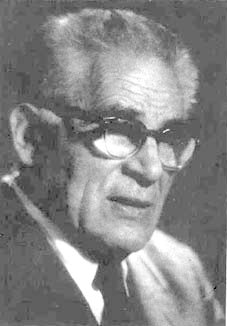
\includegraphics[width=10em]{graphics/mordell}
\end{center}
\caption{Louis J. Mordell\index{Mordell}}
\end{figure}
Let~$E$ be an elliptic curve defined over $\Q$.  The following
is a deep theorem about the group $E(\Q)$.
\begin{theorem}[Mordell]\label{thm:mordell}\ithm{Mordell}
The group $E(\Q)$ is finitely generated.
That is, there are points $P_1,\ldots, P_s \in E(\Q)$
such that every element of $E(\Q)$ is of the form $n_1 P_1 + \cdots +
n_s P_s$ for integers $n_1, \ldots n_s\in\Z$.
\end{theorem}
Mordell's theorem implies that it makes sense to ask whether or not we
can compute $E(\Q)$, where by ``compute'' we mean find a finite set
$P_1,\ldots, P_s$ of points on~$E$ that generate $E(\Q)$ as an abelian
group.  There is a systematic approach to computing $E(\Q)$ called
``descent'' (see, for example, \cite{cremona:algs, mwrank,
  silverman:aec}).  It is widely believed that the method of descent
will always succeed, but nobody has yet proved that it will.  Proving
that descent works for all curves is one of the central open problems
in number theory, and is closely related to the Birch and
Swinnerton-Dyer conjecture (one of the Clay Math Institute's million
dollar prize problems).  The crucial difficulty amounts to deciding
whether or not certain explicitly given curves have any rational
points on them or not (these are curves that have points over~$\R$ and
modulo~$n$ for all~$n$).

The details of using descent to compute $E(\Q)$ are beyond the scope
of this book. In several places below, we will simply assert that
$E(\Q)$ has a certain structure or is generated by certain elements.
In each case, we computed $E(\Q)$ using a computer implementation of
this method.

\subsection{The Torsion Subgroup of $E(\Q)$}
\index{elliptic curve!torsion subgroup} \index{torsion subgroup} For
any abelian group $G$, let $G_{\tor}$ be the subgroup of elements of
finite order.  If $E$ is an elliptic curve over $\Q$, then
$E(\Q)_{\tor}$ is a subgroup of $E(\Q)$, which must be finite because
of Theorem~\ref{thm:mordell} (see \exref{ch:ec}{ex:ector}).  One can
also prove that $E(\Q)_{\tor}$ is finite by showing that there is a
prime $p$ and an injective reduction homomorphism $E(\Q)_{\tor} \hra
E(\Z/p\Z)$, then noting that $E(\Z/p\Z)$ is finite.  For example,
if~$E$ is $y^2= x^3-5x+4$, then $ E(\Q)_{\tor} = \{\O, (1,0)\} \isom
\zmod{2}.$

The possibilities for $E(\Q)_{\tor}$ are known.
\begin{theorem}[Mazur, 1976]\ithm{Mazur}
Let~$E$ be an elliptic curve over~$\Q$.  Then $E(\Q)_{\tor}$ is
isomorphic to one of the following 15 groups:
\begin{align*}
\zmod{n} & \qquad\text{ for } n\leq 10 \text{ or } n=12,\\
\Z/2\Z\cross \Z/2n &\qquad \text{ for } n \leq 4.
\end{align*}
\end{theorem}


\begin{sg}
We compute the structure of the torsion subgroups of some elliptic curves.
In each case, the output of the function $T(a,b)$ below is a pair $c,d \in \Z$
(or integer $c$)
such that the torsion subgroup of $y^3 = x^3 + ax + b$ is
$\Z/c\Z \cross \Z/d\Z$.
\begin{verbatim}
sage: T = lambda v: EllipticCurve(v
...          ).torsion_subgroup().invariants()
sage: T([-5,4])
(2,)
sage: T([-43,166])
(7,)
sage: T([-4,0])
(2, 2)
sage: T([-1386747, 368636886])
(2, 8)
\end{verbatim}
\end{sg}


\subsection{The Rank of $E(\Q)$}
The quotient $E(\Q)/E(\Q)_{\tor}$ is a finitely generated free abelian
group, so it is isomorphism to $\Z^r$ for some integer~$r$, called the
\defn{rank} of $E(\Q)$.  For example, one can prove that if
$E$ is $y^2=x^3-5x+4$, then $E(\Q)/E(\Q)_{\tor}$ is generated by the
point $(0,2)$.

\begin{sg}
We use Sage to compute the ranks of some elliptic curves $y^2 = x^3 + ax + b$.
The function $r(a,b)$ below returns the rank of this curve over $\Q$.
\begin{verbatim}
sage: r = lambda v: EllipticCurve(v).rank()
sage: r([-5,4])
1
sage: r([0,1])
0
sage: r([-3024, 46224])
2
sage: r([-112, 400])
3
sage: r([-102627, 12560670])
4
\end{verbatim}
\end{sg}

The following is a folklore conjecture, not associated with any
particular mathematician:
\begin{conjecture}\label{ref:rankconj}\index{rank}\index{elliptic curve!rank}
There are elliptic curves over~$\Q$ of arbitrarily large rank.
\end{conjecture}

The world record \index{largest known!elliptic curve rank}
is the following curve, whose rank is at least $28$:
\begin{align*}
y^2 + &xy + y = x^3 - x^2 - \\
   & 20067762415575526585033208209338542750930230312178956502x + \\
   & 344816117950305564670329856903907203748559443593191803612\ldots\\
   & \ldots 66008296291939448732243429
\end{align*}

It was discovered in May 2006 by Noam Elkies of Harvard
University.
%\begin{align*}
%y^2 + &xy + y = x^3 - 120039822036992245303534619191166796374x\\
%         &        + 504224992484910670010801799168082726759443756222911415116
%\end{align*}
%It was discovered
%in January 2000 by Roland Martin\index{Martin} and
%William McMillen\index{McMillen} of the
%National Security Agency\index{National Security Agency}.


\subsection{The Congruent Number Problem}\label{sec:congnumprob}
\index{congruent number!problem}\index{open problem!congruent numbers}
\begin{definition}[Congruent Number]
We call a nonzero rational number~$n$ a \defn{congruent number} if
$\pm n$ is the area of a right triangle with rational
side lengths.  Equivalently,~$n$ is a \defn{congruent number} if the
system of two equations
\begin{eqnarray*}
a^2+b^2&=&c^2\\
\frac{1}{2}ab&=&n
\end{eqnarray*}
has a solution with $a,b,c\in\Q$.
\end{definition}
For example,~$6$ is the area of the right triangle with side lengths~$3$,~$4$,
and~$5$, so~$6$ is a congruent number.
Less obvious is that~$5$
is also a congruent number; it is the area of the right triangle
with side lengths $3/2$, $20/3$,  and $41/6$.  It is nontrivial
to prove that~$1$,~$2$,~$3$, and~$4$ are not congruent numbers.
Here is a list of the integer
congruent numbers\index{congruent number!all $\leq 50$ are}
up to $50$:
{
$$
5, 6, 7, 13, 14, 15, 20, 21, 22, 23, 24, 28, 29, 30, 31, 34, 37, 38, 39, 41, 45, 46, 47.
$$
}

Every congruence class modulo~$8$ except~$3$ is represented in this
list, which incorrectly suggests that if $n\con 3\pmod{8}$ then $n$ is
not a congruent number.  Though no $n\leq 218$ with $n\con 3\pmod{8}$
is a congruent number, $n=219$ is a congruent number and
$219\con 3\pmod{8}$.


Deciding whether an integer~$n$ is a congruent number can be subtle,
since the simplest triangle with area~$n$ can be very complicated.
For example, as Zagier\index{Zagier} pointed out,
the number $157$ is a congruent number\index{congruent number!157 is}, and
the ``simplest'' rational right triangle with area $157$
has side lengths
$$
 a = \frac{6803298487826435051217540}{411340519227716149383203}
\,\, \text{and} \,\,
 b = \frac{411340519227716149383203}{21666555693714761309610}.
$$
This solution would be difficult to find by a brute force search.

\index{congruent number!why called congruent} We call congruent
numbers ``congruent'' because of the following proposition,
which asserts that any congruent number is the common
``congruence'' between three perfect squares.
\begin{proposition}
Suppose~$n$ is the area of a right
triangle with rational side lengths $a, b, c$, with
$a\leq b<c$.
Let $A=(c/2)^2$.  Then
$$A-n, \quad A,\, \text{ and } A+n$$
are all perfect squares of rational numbers.
\end{proposition}\index{congruent number!and arithmetic progression}
\begin{proof}
We have
\begin{eqnarray*}
a^2+b^2&=&c^2\\
\frac{1}{2}ab&=&n
\end{eqnarray*}
Add or subtract $4$ times the second equation to the first to get
\begin{eqnarray*}
a^2\pm2ab +b^2&=&c^2\pm 4n\\
(a\pm b)^2 &=& c^2 \pm 4n\\
\left(\frac{a\pm b}{2}\right)^2 &=&
   \left( \frac{c}{2}\right)^2 \pm n \\
  &=& A \pm n
\end{eqnarray*}
\end{proof}

The main motivating open problem related to congruent numbers
is to give a systematic way to recognize them.
\begin{openproblem}\label{prob:cong}
\index{open problem!decide if congruent number}
Give an algorithm which, given~$n$, outputs whether or
not~$n$ is a congruent number.
\end{openproblem}

\index{elliptic curve!and congruent numbers}
\index{congruent number!and elliptic curves}
Fortunately, the vast theory developed about elliptic curves
has something to say about the above problem.  In order to understand
this connection, we begin with an elementary algebraic proposition
that establishes a link between elliptic curves
and the congruent number problem.
\begin{proposition}[Congruent numbers and elliptic curves]\label{prop:congbij}%
\iprop{congruent numbers and elliptic curves}
Let~$n$ be a rational number.   There is a bijection between
$$
 A = \left\{(a,b,c) \in \Q^3 \,:\, \frac{ab}{2} = n,\, a^2 + b^2 = c^2\right\}
$$
and
$$
 B = \left\{(x,y) \in \Q^2 \,:\, y^2 = x^3 - n^2 x, \,\,\text{\rm with } y \neq 0\right\}
$$
given explicitly by the maps
$$
  f(a,b,c) = \left(-\frac{nb}{a+c},\,\, \frac{2n^2}{a+c}\right)
$$
and
$$
  g(x,y) = \left(\frac{n^2-x^2}{y},\,\,
                         -\frac{2xn}{y},\,\, \frac{n^2+x^2}{y}\right).
$$
\end{proposition}
The proof of this proposition is not deep, but involves substantial
(elementary) algebra and we will not prove it in this book.

For $n\neq 0$, let $E_n$ be the elliptic curve $y^2 = x^3 - n^2 x$.
\begin{proposition}[Congruent number criterion]%
\iprop{congruent number criterion}%
  The rational number~$n$ is a congruent number if and only if
there is a point $P=(x,y)\in E_n(\Q)$ with $y\neq 0$.
\end{proposition}
\begin{proof}
The number~$n$ is a congruent number if and only if the set~$A$ from
Proposition~\ref{prop:congbij} is nonempty.  By the proposition~$A$ is
nonempty if and only if~$B$ is nonempty.
\end{proof}

\begin{example}\label{ex:cong5}
Let $n=5$.  Then $E_n$ is $y^2=x^3-25x$, and we notice
that $(-4,-6)\in E_n(\Q)$.  We next use the bijection
of Proposition~\ref{prop:congbij} to find the corresponding
right triangle:
$$
  g(-4,-6) = \left(\frac{25-16}{-6},-\frac{-40}{-6}, \frac{25+16}{-6}\right)
           = \left(-\frac{3}{2}, -\frac{20}{3}, -\frac{41}{6}\right).
$$
Multiplying through by~$-1$ yields the side lengths of a rational
right triangle with area~$5$.  {\em Are there any others?}

Observe that we can apply~$g$ to any point in $E_n(\Q)$ with $y\neq 0$.
Using the group law, we find that $2(-4,-6) = (1681/144, 62279/1728)$
and
$$
  g(2(-4,-6)) = \left(
-\frac{1519}{492}, -\frac{4920}{1519}, \frac{3344161}{747348}
\right).
$$
This example foreshadows Theorem~\ref{thm:inftri}.
\end{example}

\begin{example}
Let $n=1$, so $E_1$ is defined by $y^2=x^3-x$.  Since~$1$ is not
a congruent number, the elliptic curve $E_1$ has no point
with $y\neq 0$.  See \exref{ch:ec}{ex:cong1}.
\end{example}

\begin{sg}
  We implement the {\tt cong} function in Sage, which returns a triple
  $(a,b,c)$ whose entries are the sides of a rational right triangle
  of area $n$ if one exists, and returns False if there are no such
  triangles.
\begin{verbatim}
sage: def cong(n):
...       G = EllipticCurve([-n^2,0]).gens()
...       if len(G) == 0: return False
...       x,y,_ = G[0]
...       return ((n^2-x^2)/y,-2*x*n/y,(n^2+x^2)/y)
sage: cong(6)
(3, 4, 5)
sage: cong(5)
(3/2, 20/3, 41/6)
sage: cong(1)
False
sage: cong(13)
(323/30, 780/323, 106921/9690)
sage: (323/30 * 780/323)/2
13
sage: (323/30)^2 + (780/323)^2 == (106921/9690)^2
True
\end{verbatim}
\end{sg}


\begin{theorem}[Infinitely Many Triangles]\ithm{infinitely many triangles}\label{thm:inftri}
If $n$ is a congruent number, then there are infinitely
many distinct right triangles with rational side lengths
and area~$n$.
\end{theorem}
We will not prove this theorem, except to note that one proves it by showing that
$E_n(\Q)_{\tor} = \{\O,(0,0),(n,0),(-n,0)\}$, so the
elements of the set $B$ in Proposition~\ref{prop:congbij} all have
infinite order. Hence, $B$ is infinite
so $A$ is infinite.


Tunnell has proved that the Birch and Swinnerton-Dyer conjecture
(alluded to above), implies the existence of an elementary way to
decide whether or not an integer~$n$ is a congruent number.  We state
Tunnell's elementary way in the form of a conjecture.
\begin{conjecture}\label{conj:cong}
Let $a,b,c$ denote integers.
If~$n$ is an even square-free integer, then
$n$ is a congruent number if and only if
$$
\#\left\{(a,b,c)\in\Z^3 : 4a^2 + b^2 + 8c^2 = \frac{n}{2} : c\text{\rm{} is even}\right\}$$
$$
  \qquad\qquad\qquad\qquad\qquad   =
  \#\left\{(a,b,c) : 4a^2 + b^2 + 8c^2 = \frac{n}{2}: c\text{\rm{} is odd}\right\}.$$
If~$n$ is odd and square free then
$n$ is a congruent number if and only if
$$\#\left\{(a,b,c) : 2a^2 + b^2 + 8c^2 = n : c\text{\rm{} is even}\right\}$$
$$  \qquad\qquad\qquad\qquad\qquad =
    \#\left\{(a,b,c) : 2a^2 + b^2 + 8c^2 = n: c\text{\rm{} is odd}\right\}.$$
\end{conjecture}

Enough of the Birch and Swinnerton-Dyer conjecture is known to prove
one direction of Conjecture~\ref{conj:cong}.  In particular, it is a
very deep theorem that if we do not have equality of the displayed
cardinalities, then~$n$ is not a congruent
number.


The even more difficult (and still open!) part of
Conjecture~\ref{conj:cong} is the converse: If one has equality of the
displayed cardinalities, prove that $n$ is a congruent number.  The
difficulty in this direction, which appears to be very deep, is that
we must somehow construct (or prove the existence of) elements of
$E_n(\Q)$.  This has been accomplished in some cases due to the
groundbreaking work of Gross and Zagier (\cite{gross-zagier}) but much
work remains to be done.

The excellent book \cite{koblitz:cong} is about congruent numbers and
Conjecture~\ref{conj:cong}, and we encourage the reader to consult it.
The Birch and Swinnerton-Dyer conjecture is a Clay Math Institute
million dollar millennium prize problem (see \cite{cmi, wiles:cmi}).


\begin{exercises}
\item\label{ex:singgrp} Write down an equation $y^2 = x^3 +ax + b$ over a field
$K$ such that $-16(4a^3+27b^2)= 0$.  Precisely what goes wrong
when trying to endow the set
$E(K) = \{ (x,y)\in K\cross K : y^2 = x^3 + ax +b \} \union \{\O\}$
with a group structure?

\item\label{ex:ell2} One rational solution to the equation
$y^2=x^3-2$ is $(3,5)$.  Find a rational solution with $x\neq 3$ by
drawing the tangent line to $(3,5)$ and computing the second point of
intersection.

\item\label{ex:ell4}
Let~$E$ be the elliptic curve over the finite
field $K=\Z/5\Z$ defined by the equation
$$
y^2 = x^3 + x +1.
$$
\begin{enumerate}
\item List all~$9$ elements of~$E(K)$.
\item What is the structure of
$E(K)$, as a product of cyclic groups?
\end{enumerate}

\item\label{ex:ell11}
Let~$E$ be the elliptic curve
defined by the equation $y^2 = x^3 +1$.
For each prime $p\geq 5$, let $N_p$ be the cardinality of the group
$E(\zmod{p})$ of points on this curve having coordinates
in $\zmod{p}$.  For example, we have that
$N_{5} = 6, N_{7} = 12, N_{11} = 12, N_{13} = 12,
N_{17} = 18, N_{19} = 12, , N_{23} = 24, \text{ and }N_{29} = 30$
(you do not have to prove this).
\begin{enumerate}
\item  For the set of primes satisfying $p\con 2\pmod{3}$, can you see a
  pattern for the values of $N_p$?  Make a general conjecture for the
  value of $N_p$ when $p\con 2\pmod{3}$.
\item (*) Prove your conjecture.
\end{enumerate}

\item\label{ex:ell13}
Let~$E$ be an elliptic curve over the real numbers~$\R$.
Prove that $E(\R)$ is not a finitely generated abelian group.

%\item
%The Hasse bound for $p=5$ asserts that if $E$
%is an elliptic curve over $\Z/5\Z$,
%then $|\#E(\Z/5\Z) - 6| \leq 4$.

\item\label{ex:ector} (*)
Suppose $G$ is a finitely generated abelian group.
Prove that the subgroup $G_{\tor}$ of elements of finite
order in $G$ is finite.


\item \label{ex:elltrans}
 Suppose $y^2=x^3+ax+b$ with $a,b\in\Q$ defines an elliptic
curve.  Show that there is another equation $Y^2=X^3+AX+B$ with
$A,B\in\Z$ whose solutions are in bijection with the
solutions to $y^2=x^3+ax+b$.


\item\label{ex:pythag} Suppose $a$, $b$, $c$ are relatively prime
  integers with $a^2+b^2=c^2$.  Then there exist integers $x$ and $y$
  with $x>y$ such that $c=x^2+y^2$ and either $a=x^2-y^2$, $b=2xy$ or
  $a=2xy$, $b=x^2-y^2$.


\item\label{ex:flt4}(*) Fermat's Last Theorem for exponent $4$ asserts
  that any solution to the equation $x^4+y^4=z^4$ with $x,y,z\in\Z$
  satisfies $xyz=0$.  Prove Fermat's Last
  Theorem for exponent $4$, as follows.
\begin{enumerate}
\item Show that if the equation $x^2+y^4=z^4$ has no integer solutions
  with $xyz\neq 0$, then Fermat's Last Theorem for exponent~$4$ is
  true.
\item Prove that $x^2+y^4=z^4$ has no integer solutions with $xyz\neq
  0$ as follows.  Suppose $n^2+k^4=m^4$ is a solution with $m>0$
  minimal among all solutions.  Show that there exists a solution with
  $m$ smaller using \exref{ch:ec}{ex:pythag} (consider two cases).
\end{enumerate}

\item \label{ex:bpowersmooth}
This problem requires a computer.
\begin{enumerate}
\item Show that the set of numbers $59+1\pm
s$ for $s\leq 15$ contains~$14$ numbers that are $B$-power smooth
for~$B=20$.
\item
Find the proportion of primes~$p$ in the interval
from $10^{12}$ and $10^{12}+1000$ such that $p-1$ is
$B=10^5$ power smooth.
\end{enumerate}

\item\label{ex:cong1}(*) Prove that $1$ is not a congruent number by
  showing that the elliptic curve $y^2=x^3-x$ has no rational
  solutions except $(0,\pm 1)$ and $(0,0)$, as follows:
\begin{enumerate}
\item Write $y=\frac{p}{q}$ and $x=\frac{r}{s}$, where $p,q,r,s$ are
all positive integers and $\gcd(p,q)=\gcd(r,s)=1$.  Prove that $s\mid
q$, so $q=sk$ for some $k\in\Z$.
\item Prove that $s=k^2$, and substitute to see that
$p^2=r^3-rk^4$.
\item Prove that $r$ is a perfect square by supposing that there is a
  prime~$\ell$ such that $\ord_{\ell}(r)$ is odd, and analyzing
  $\ord_{\ell}$ of both sides of $p^2=r^3-rk^4$.
\item Write $r=m^2$, and substitute to
see that $p^2=m^6-m^2k^4$. Prove that $m\mid p$.
\item Divide through by $m^2$ and deduce a contradiction
to \exref{ch:ec}{ex:flt4}.
\end{enumerate}

\end{exercises}

\chapter*{Answers and Hints}
\addcontentsline{toc}{chapter}{\numberline{}Answers and Hints}
\newcommand{\chapitem}[2]{\vspace{2ex}\item {\large \bf #1. #2}}
\begin{itemize}
\chapitem{Chapter 1}{Prime Numbers}
\begin{enumerate}
\item[\ref{ex:handsieve}.] They are
$2, 3, 5, 7, 11, 13, 17, 19, 23, 29, 31, 37, 41, 43, 47, 53, 59,$\\
$61, 67, 71, 73, 79, 83, 89, 97$.
\item[\ref{ex:primesform}.] Emulate the proof of Proposition~\ref{prop:4x-1}.
\end{enumerate}

\chapitem{Chapter 2}{The Ring of Integers Modulo $n$}
\begin{enumerate}
\item[\ref{ex:gcds}.] They are $5$, $13$, $3$, and $8$.
\item[\ref{ex:gcdrep}.] For example, $x=22$, $y=-39$.

\item[\ref{ex:binomdiv}.] Hint: Use the binomial theorem
and prove that if $r\geq 1$, then $p$ divides
$\binom{p}{r}$.

\item[\ref{ex:residues}.] For example,
$S_1 = \{0,1,2,3,4,5,6\}$, $S_2 = \{1,3,5,7,9,11,13\}$,
$S_3 = \{0,2,4,6,8,10,12\}$, and $S_4 = \{2,3,5,7,11,13,29\}.$
In each we find $S_i$ by listing the first seven numbers
satisfying the $i$th condition, then adjust the last number if
necessary so that the reductions will be distinct modulo $7$.
\item[\ref{ex:divrules}.] An integer is divisible by $5$ if
and only if the last digits is $0$ or $5$.  An integer is
divisible by $9$ if and only if the sum of the digits is
divisible by $9$.  An integer is divisible by $11$ if and only
if the alternating sum of the digits is divisible by $11$.
\item[\ref{ex:putnam98}.] Hint for part (a): Use the divisibility rule
you found in \exref{ch:prime}{ex:divrules}.

\item[\ref{ex:invmod}.] $71$

\item[\ref{ex:ordmod}.] $8$

\item[\ref{ex:zpfield}.] As explained on page~\pageref{page:znring},
we know that $\zmod{n}$ is a ring for any $n$.  Thus to show that
$\zmod{p}$ is a field it suffices to show that every nonzero element
$\overline{a}\in\zmod{p}$ has an inverse.  Lift $a$ to an element $a\in\Z$,
and set $b=p$ in Proposition~\ref{prop:xgcd}.   Because $p$ is prime,
$\gcd(a,p)=1$, so there exists $x,y$ such that $ax + py = 1$.
Reducing this equality modulo $p$ proves that $\overline{a}$ has
an inverse $x\pmod{p}$.  Alternatively, one could argue just
like after Definition~\ref{defn:order} that $\overline{a}^m=1$
for some $m$, so some power of $\overline{a}$ is the
inverse of $\overline{a}$.

\item[\ref{ex:crt}.] $302$

\item[\ref{ex:phiodd}.] Only for $n=1,2$.  If $n>2$, then
$n$ is either divisible by an odd prime $p$ or $4$.  If $4\mid n$,
then $2^e-2^{e-1}$ divides $\vphi(n)$ for some $e\geq 2$, so $\vphi(n)$
is even.  If an odd $p$ divides $n$, then the even number
$p^e-p^{e-1}$ divides $\vphi(n)$ for some $e\geq 1$.

\item[\ref{ex:multproof2}.]  The map $\psi$ is a homomorphism since
both reduction maps $$\zmod{mn}\to \zmod{m}\quad\text{and}\quad
\zmod{mn}\to \zmod{n}$$
are homomorphisms.  It is injective because if $a\in\Z$ is such
that $\psi(a)=0$, then $m\mid a$ and $n\mid a$, so $mn\mid a$ (since
$m$ and $n$ are coprime), so $a\con 0\pmod{mn}$.
The cardinality of $\zmod{mn}$ is $mn$ and the cardinality of
the product $\zmod{m}\times \zmod{n}$ is also $mn$, so $\psi$
must be an isomorphism.  The units $(\zmod{mn})^*$ are thus
in bijection with the units $(\zmod{m})^*\times (\zmod{n})^*$.

For the second part of the exercise, let $g=\gcd(m,n)$ and
set $a=mn/g$.  Then $a\not\con 0\pmod{mn}$, but $m\mid a$ and
$n\mid a$, so $a\ker(\psi)$.

\item[\ref{ex:thieves}.] We express the question as a
system of linear equations modulo various numbers, and use the Chinese
remainder theorem.    Let $x$ be the number of books.
The problem asserts that
\begin{align*}
x&\con 6\pmod{7}\\
x&\con 2\pmod{6}\\
x&\con 1\pmod{5}\\
x&\con 0\pmod{4}
\end{align*}
Applying CRT to the first pair of equations, we find that
$x\con 20\pmod{42}$.  Applying CRT to this equation and
the third, we find that $x\con 146\pmod{210}$.  Since $146$
is not divisible by $4$, we add multiples of $210$ to $146$
until we find the first $x$ that is divisible by $4$.  The first multiple
works, and we find that the aspiring mathematicians
have $356$ math books.

\item[\ref{ex:pcube}.]  Note that $p=3$ works, since $11=3^2+2$ is prime.
Now suppose $p\neq 3$ is any prime such that $p$ and $p^2+2$ are both prime.
We must have $p\con 1\pmod{3}$ or $p\con 2\pmod{3}$.
Then $p^2\con 1\pmod{3}$, so $p^2+2\con 0\pmod{3}$.
Since $p^2 + 2 $ is prime, we must have $p^2 + 2 = 3$, so $p=1$,
a contradiction as $p$ is assumed prime.

\item[\ref{ex:phimult}.]
For (a) $n=1,2$, see solution to \exref{ch:cong}{ex:phiodd}.
For (b), yes there are many such examples.  For example, $m=2$, $n=4$.

\item[\ref{ex:phiformula}.]
By repeated application of multiplicativity and Equation (\ref{eqn:phipower})
on page~\pageref{eqn:phipower}, we see that if $n=\prod_i p_i^{e_i}$
is the prime factorization of $n$, then
$$
   \vphi(n) = \prod_i (p_i^{e_i} - p_i^{e_i-1})
   = \prod_i p_i^{e_i-1} \cdot \prod_i (p_i-1).
$$

\item[\ref{ex:solnsqrtmod35}.] 1, 6, 29, 34

\item[\ref{ex:reducedfraction}.]
Let $g=\gcd(12n+1,30n+2)$.   Then $g\mid 30n+2 - 2\cdot (12n+1) = 6n$.
 For the same reason, $g$ also divides
$12n+1 - 2\cdot (6n) = 1$, so $g=1$, as claimed.

\item[\ref{ex:prim1}.]  There is no primitive
root modulo $8$, since $(\zmod{8})^*$ has order $4$,
but every element of $(\zmod{8})^*$ has order $2$.
Prove that if $\zeta$ is a primitive root modulo $2^n$, for
$n\geq 3$, then the reduction of $\zeta$ mod $8$ is a primitive
root, a contradiction.

\item[\ref{ex:prim2}.] $2$ is a primitive root modulo $125$.


\item[\ref{ex:prim_fac}.] Let $\prod_{i=1}^m p_i^{e_i}$ be the prime
factorization of $n$.  Slightly
generalizing Exercise~\ref{ex:multproof2}, we see that
$$
  (\zmod{n})^* \isom \prod (\zmod{p_i^{e_i}})^*.
$$
Thus $(\zmod{n})^*$ is cyclic if and only if the product
$(\zmod{p_i^{e_i}})^*$ is cyclic.  If $8\mid n$, then
there is no chance $(\zmod{n})^*$ is cyclic, so assume
$8\nmid n$.  Then by \exref{ch:cong}{ex:prim2},
each group $(\zmod{p_i^{e_i}})^*$ is itself cyclic.
A product of cyclic groups is cyclic if and only
the orders of the factors in the product are coprime (this
follows from \exref{ch:cong}{ex:multproof2}).
Thus $(\zmod{n})^*$ is cyclic if and only if the numbers
$p_i(p_i-1)$, for $i=1,\ldots, m$ are pairwise coprime.
Since $p_i-1$ is even, there can be at most one odd
prime in the factorization of $n$, and we see that
$(\zmod{n})^*$ is cyclic if and only if $n$ is an odd
prime power, twice an odd prime power, or $n=4$.

\end{enumerate}


\chapitem{Chapter 3}{Public-Key Cryptography}
\begin{enumerate}
\item[\ref{ex:crypto2}.] The best case is that each letter is A.
Then the question is to find the largest $n$ such that
$1 + 27 + \cdots + 27^n \leq 10^{20}$.
By computing $\log_{27}(10^{20})$, we see that
$27^{13}<10^{20}$ and $27^{14}>10^{20}$.  Thus $n\leq 13$,
and since $1 + 27  + \cdots + 27^{n-1} < 27^n$, and
$2\cdot 27^{13}<10^{20}$, it follows that $n=13$.

\item[\ref{ex:crypto6}.] This is not secure, since it is just
equivalent to a ``Ceaser Cipher,'' that is a permutation
of the letters of the alphabet, which is well-known to be
easily broken using a frequency analysis.

\item[\ref{ex:crack3}.] If we can compute the polynomial
$$f = (x-p)(x-q)(x-r)
  = x^3 - (p+q+r)x^2 + (pq+pr+qr)x - pqr,
$$
then we can factor $n$ by finding the roots of $f$, for example, using
Newton's method (or Cardona's formula for the roots of a cubic).
Because $p$, $q$,~$r$, are distinct odd primes, we have
$$\vphi(n) =(p-1)(q-1)(r-1) = pqr-(pq+pr+qr)+p+q+r,$$
and
$$\sigma(n) = 1 + (p+q+r)+(pq+pr+qr) + pqr.$$
Since we know $n$, $\vphi(n)$, and $\sigma(n)$, we know
\begin{align*}
\sigma(n)-1-n &= (p+q+r)+(pq+pr+qr),\quad\text{and}\\
\vphi(n)-n    &= (p+q+r)-(pq+pr+qr).
\end{align*}
We can thus compute
both $p+q+r$ and $pq+pr+qr$, hence deduce~$f$
and find $p,q,r$.
\end{enumerate}

\chapitem{Chapter 4}{Quadratic Reciprocity}
\begin{enumerate}
\item[\ref{ex:rec1}.]  They are all $1$, $-1$, $0$, and $1$.

\item[\ref{ex:rec2}.]  By Proposition~\ref{prop:euler_prop},
the value of $\kr{3}{p}$ depends
only on the reduction $\pm p\pmod{12}$.  List enough primes~$p$ such that
$\pm p$ reduce to $1,5,7,11$ modulo $12$ and verify that
the asserted formula holds for each of them.

\item[\ref{ex:rec9}.] Since $p=2^{13}-1$ is prime, there
are either two solutions or no solutions to $x^2\con 5\pmod{p}$,
and we can decide which using quadratic reciprocity.
We have
$$\kr{5}{p} = (-1)^{(p-1)/2\cdot (5-1)/2}\kr{p}{5} = \kr{p}{5},$$
so there are two solutions if and only if $p=2^{13}-1$ is $\pm 1$
mod~$5$.  In fact, $p\con 1\pmod{5}$, so there are two solutions.

\item[\ref{ex:rec10}.] We have $4^{48} = 2^{96}$.
By Euler's Theorem, $2^{96}=1$, so $x=1$.

\item[\ref{ex:rec13}.] For (a), take $a=19$ and $n=20$.  We
found this example using the Chinese remainder theorem applied
to $4\pmod{5}$ and $3\pmod{4}$, and used that
$\kr{19}{20} = \kr{19}{5}\cdot\kr{19}{4} = (-1)(-1)=1$,
yet $19$ is not a square modulo either $5$ or $4$, so is
certainly not a square modulo $20$.

\item[\ref{ex:rec14}.]  Hint: First reduce to the case that $6k-1$ is
  prime, by using that if $p$ and $q$ are primes not of the form
  $6k-1$, then neither is their product.  If $p=6k-1$ divides
  $n^2+n+1$, it divides $4n^2+4n+4 = (2n+1)^2+3$, so $-3$ is a
  quadratic residue modulo~$p$.  Now use quadratic reciprocity to show
  that $-3$ is not a quadratic residue modulo~$p$.


\end{enumerate}

\chapitem{Chapter 5}{Continued Fractions}
\begin{enumerate}
\item[\ref{ex:qf4}.] Suppose $n=x^2+y^2$, with $x,y\in\Q$.  Let $d$ be
  such that $dx, dy\in\Z$.  Then $d^2 n = (dx)^2 + (dy)^2$ is a sum of
  two integer squares, so by Theorem~\ref{thm:sumsquare}, if $p\mid d^2
  n$ and $p\con 3\pmod{4}$, then $\ord_p(d^2n)$ is even.  We have
  $\ord_p(d^2n)$ is even if and only if $\ord_p(n)$ is even, so
  Theorem~\ref{thm:sumsquare} implies that $n$ is also a sum of two
  squares.

\item[\ref{ex:qf7}.] The squares modulo $8$ are $0,1,4$, so a sum
of two squares reduces modulo $8$ to one of $0,1,2,4$, or $5$.
Four consecutive integers that are sums of squares would reduce to
four consecutive integers in the set $\{0,1,2,4,5\}$, which
is impossible.
\end{enumerate}

\chapitem{Chapter 6}{Elliptic Curves}
\begin{enumerate}
\item[\ref{ex:ell2}.] The second point of intersection is
$(129/100, 383/1000)$.

\item[\ref{ex:ell4}.] The group is cyclic of order $9$, generated
by $(4,2)$.  The elements of $E(K)$ are
$$\{\O, (4,2), (3,4), (2,4), (0,4), (0,1), (2,1), (3,1), (4,3)\}.$$

\item[\ref{ex:ell11}.]  In part (a), the pattern is that $N_p=p+1$.
For part (b), a hint is that when $p\con 2\pmod{3}$,
the map $x\mapsto x^3$ on $(\zmod{p})^*$ is an automorphism,
so $x\mapsto x^3+1$ is a bijection.  Now use what you learned
about squares in $\zmod{p}$ from Chapter~\ref{ch:reciprocity}.

\item[\ref{ex:ell13}.] For all sufficiently large real $x$, the
equation $y^2=x^3+ax+b$ has a real solution $y$.  Thus, the
group $E(\R)$ is not countable, since $\R$ is not countable.
But any finitely generated group is countable.

\item[\ref{ex:ector}.] In a course on abstract algebra, one often
  proves the nontrivial fact that every subgroup of a finitely
  generated abelian group is finitely generated.  In particular, the
  torsion subgroup $G_{\tor}$ is finitely generated.  However, a
  finitely generated abelian torsion group is finite.

\item[\ref{ex:elltrans}.]
Hint: Multiply both sides of $y^2=x^3+ax+b$ by a power of a common
denominator, and ``absorb'' powers into~$x$ and~$y$.

\item[\ref{ex:pythag}.] Hint: see \exref{ch:reciprocity}{ex:rec8}.

\end{enumerate}


\end{itemize}
